% ****************************************************************************************** % Dissertation template and document class for Princeton University
% Author  : Jeffrey Scott Dwoskin <jdwoskin@princeton.edu>
% Adapted from: http://www.math.princeton.edu/graduate/tex/puthesis.html
% ****************************************************************************************** %


%%% For print copies
%% set 'singlespace' option to set entire thesis to single space, and define "\printmode" to remove all hyperlinks for printed copies of the thesis. Delete all output files before changing this mode -- it will turn hyperref package on and off
%\documentclass[12pt,lot, lof, singlespace]{puthesis}
%\newcommand{\printmode}{}

%%% For the electronic copy, use doublespacing, define "\proquestmode" to use outlined links, instead of colored links. 
%\documentclass[12pt,lot, lof]{puthesis}
\documentclass[12pt]{puthesis}
\newcommand{\proquestmode}{}

% I prefer proquestmode to be off for electronic copies for normal use, since the colored links are less distracting. However when printed in black and white, the colored links are difficult to read. 

%%% For early drafts without some of the frontmatter
% Also see the "ifodd" command below to disable more frontmatter
%\documentclass[12pt]{puthesis}

%%%%%%%%%%%%%%%%%%%%%%%%%%%%%%%%%%%%%%%%%%%%%%%%%%%%%%%%%%%%%\
%%%% Author & title page info

\title{Transport Experiments of Topological Insulators and Dirac Semimetals}

\submitted{April 2016}  % degree conferral date (January, April, June, September, or November)
\copyrightyear{2016}  % year in which the copyright is secured by publication of the dissertation.
\author{Jun Xiong}
\adviser{Professor Nai Phuan Ong}  %replace with the full name of your adviser
%\departmentprefix{Program in}  % defaults to "Department of", but programs need to change this.
\department{Physics}

%%%%%%%%%%%%%%%%%%%%%%%%%%%%%%%%%%%%%%%%%%%%%%%%%%%%%%%%%%%%%\
%%%% Tweak float placements
% From: http://mintaka.sdsu.edu/GF/bibliog/latex/floats.html "Controlling LaTeX Floats"
% and based on: http://www.tex.ac.uk/cgi-bin/texfaq2html?label=floats
% LaTeX defaults listed at: http://people.cs.uu.nl/piet/floats/node1.html

% Alter some LaTeX defaults for better treatment of figures:
    % See p.105 of "TeX Unbound" for suggested values.
    % See pp. 199-200 of Lamport's "LaTeX" book for details.
    %   General parameters, for ALL pages:
    \renewcommand{\topfraction}{0.85}	% max fraction of floats at top
    \renewcommand{\bottomfraction}{0.6}	% max fraction of floats at bottom
    %   Parameters for TEXT pages (not float pages):
    \setcounter{topnumber}{2}
    \setcounter{bottomnumber}{2}
    \setcounter{totalnumber}{4}     % 2 may work better
    \setcounter{dbltopnumber}{2}    % for 2-column pages
    \renewcommand{\dbltopfraction}{0.66}	% fit big float above 2-col. text
    \renewcommand{\textfraction}{0.15}	% allow minimal text w. figs
    %   Parameters for FLOAT pages (not text pages):
    \renewcommand{\floatpagefraction}{0.66}	% require fuller float pages
	% N.B.: floatpagefraction MUST be less than topfraction !!
    \renewcommand{\dblfloatpagefraction}{0.66}	% require fuller float pages

% The documentclass already sets parameters to make a high penalty for widows and orphans. 

%%%%%%%%%%%%%%%%%%%%%%%%%%%%%%%%%%%%%%%%%%%%%%%%%%%%%%%%%%%%%\
%%%% Use packages

%\usepackage{amsfonts}

%%% For figures
\usepackage{graphicx}
%\usepackage{subfig,rotate}

%%% for comments
\usepackage{verbatim}

%%% For tables
\usepackage{multirow}
% Longtable lets you have tables that span multiple pages.
\usepackage{longtable}

% Booktabs produces far nicer tables than the standard LaTeX tables.
%   see: http://en.wikibooks.org/wiki/LaTeX/Tables
\usepackage{booktabs}
\usepackage{amsmath,esint, amssymb}
%\usepackage{commath}
\usepackage{gensymb}


\usepackage{dcolumn}% Align table columns on decimal point
\usepackage{bm}% bold math
\usepackage{braket}
\usepackage{caption}
\usepackage{float}
%\usepackage[utf8]{inputenc}

\newcommand{\etal}{\emph{et al.}}
\newcommand{\be}{\begin{equation}}
\newcommand{\ee}{\end{equation}}
\newcommand{\bfig}{\begin{figure}}
\newcommand{\efig}{\end{figure}}
\newcommand{\incl}{\includegraphics}
\newcommand*\VF[1]{\mathbf{#1}}
\newcommand*\dif{\mathop{}\!\mathrm{d}}


%set parameters for longtable:
% default caption width is 4in for longtable, but wider for normal tables
\setlength{\LTcapwidth}{\textwidth}



%%%%%%%%%%%%%%%%%%%%%%%%%%%%%%%%%%%%%%%%%%%%%%%%%%%%%%%%%%
%%% Printed vs. online formatting
\ifdefined\printmode

% Printed copy
% url package understands urls (with proper line-breaks) without hyperlinking them
\usepackage{url}


\else

\ifdefined\proquestmode
%ProQuest copy -- http://www.princeton.edu/~mudd/thesis/Submissionguide.pdf

% ProQuest requires a double spaced version (set previously). They will take an electronic copy, so we want links in the pdf, but also copies may be printed or made into microfilm in black and white, so we want outlined links instead of colored links.
\usepackage{hyperref}
\hypersetup{bookmarksnumbered}

% copy the already-set title and author to use in the pdf properties
\makeatletter
\hypersetup{pdftitle=\@title,pdfauthor=\@author}
\makeatother

\else
% Online copy

% adds internal linked references, pdf bookmarks, etc

% turn all references and citations into hyperlinks:
%  -- not for printed copies
% -- automatically includes url package
% options:
%   colorlinks makes links by coloring the text instead of putting a rectangle around the text.
\usepackage{hyperref}
\hypersetup{colorlinks,bookmarksnumbered}

% copy the already-set title and author to use in the pdf properties
\makeatletter
\hypersetup{pdftitle=\@title,pdfauthor=\@author}
\makeatother

% make the page number rather than the text be the link for ToC entries
%\hypersetup{linktocpage}
\fi % proquest or online formatting
\fi % printed or online formatting


%%%%%%%%%%%%%%%%%%%%%%%%%%%%%%%%%%%%%%%%%%%%%%%%%%%%%%%%%%%%%\
%%%% Define commands

% Define any custom commands that you want to use.
% For example, highlight notes for future edits to the thesis
%\newcommand{\todo}[1]{\textbf{\emph{TODO:}#1}}


% create an environment that will indent text
% see: http://latex.computersci.org/Reference/ListEnvironments
% 	\raggedright makes them left aligned instead of justified

\newenvironment{indenttext}{
    \begin{list}{}{ \itemsep 0in \itemindent 0in
    \labelsep 0in \labelwidth 0in
    \listparindent 0in
    \topsep 0in \partopsep 0in \parskip 0in \parsep 0in
    \leftmargin 1em \rightmargin 0in
    \raggedright
    }
    \item
  }
  {\end{list}}

% another environment that's an indented list, with no spaces between items -- if we want multiple items/lines. Useful in tables. Use \item inside the environment.
% 	\raggedright makes them left aligned instead of justified

\newenvironment{indentlist}{
    \begin{list}{}{ \itemsep 0in \itemindent 0in
    \labelsep 0in \labelwidth 0in
    \listparindent 0in
    \topsep 0in \partopsep 0in \parskip 0in \parsep 0in
    \leftmargin 1em \rightmargin 0in
    \raggedright
    }

  }
  {\end{list}}



%%%%%%%%%%%%%%%%%%%%%%%%%%%%%%%%%%%%%%%%%%%%%%%%%%%%%%%%%%%%%\
%%%% Front-matter

% For early drafts, you may want to disable some of the frontmatter. Simply change this to "\ifodd 1" to do so.
\ifodd 0
% front-matter disabled while writing chapters
\renewcommand{\maketitlepage}{}
\renewcommand*{\makecopyrightpage}{}
\renewcommand*{\makeabstract}{}

% you can just skip the \acknowledgements and \dedication commands to leave out these sections.

\else


\abstract{
% Abstract can be any length, but should be max 350 words for a Dissertation for ProQuest's print indicies (150 words for a Master's Thesis) or it will be truncated for those uses.
%This is a \LaTeX{} template and document class for Ph.D. dissertations at Princeton University. It was created in 2010 by Jeffrey Dwoskin, and adapted from a template provided by the math department. Their original version is available at: \url{http://www.math.princeton.edu/graduate/tex/puthesis.html}
%
%This is \textbf{NOT} an official document. Please verify the current Mudd Library dissertation requirements~\cite{mudd2009} and any department-specific requirements before using this template or document class.
%
%
%Your abstract can be any length, but should be a maximum of 350 words for a Dissertation for ProQuest's print indicies (or 150 words for a Master's Thesis); otherwise it will be truncated for those uses~\cite{proquest2006}.
%
%
%Dwoskin Ph.D. Dissertation Template --- version 1.0, 5/19/2010
%
%
%This thesis summarizes the electric transport experimental results on the bulk-insulating topological insulators and three dimensional Dirac semimetals. Unlike the traditional description of crystals, which utilizes the local symmetry, the topological insulator theory utilizes the electron wavefuntion space as a whole to distinguish different insulators. One important prediction of these theories is that topological insulators are supposed to host two-dimensional Dirac states on the surface. These surface states are spin-polarized and can serve as the bricks for novel physics such as axion electrodynamic phenomena and Majorana fermions. 

In recent years, the progress in understanding the Berry phase of Bloch electrons in crystals has triggered tremendous interest in discovering  novel topological properties and exotic phases of solids. In a crystal, the Berry curvature acts as an intrinsic magnetic field when an electron moves in the momentum space. The integration of  the Berry curvature in the Brillouin zone can categorize solids into phases such as topological insulators (TI), Chern insulators, Dirac semimetals (DSM) and Weyl semimetals (WSM). These new phases have unconventional electronic states at the boundaries. For example, a three-dimensional (3D) TI hosts spin polarized electrons on its surface, while chiral fermions live on the magnetic domain boundaries of quantum anomalous Hall phases. These Dirac-like edge states are usually protected by the time-reversal (TR) symmetry and stay immune to the backscattering. Under proper engineering, such edge states can carry a dissipationless current without a magnetic field, leading to a great application potential in low-power devices. In addition, these edge states may serve as building bricks of future topological quantum computers.

Besides TI, the newly discovered Dirac and Weyl semimetals represent another example in which electrons obey equations from high energy physics. Both a DSM and a WSM have a linear energy-momentum dispersion. Besides, a WSM hosts an even number of topologically protected Weyl nodes. The paired Weyl nodes have opposite chiralities, and can be regarded as positive and negative monopoles of the Berry flux. There are also surface Fermi arcs that connect the Weyl nodes. Under the TR, inversion and certain crystal symmetries, as in the cases of Cd$_3$As$_2$ and Na$_3$Bi, the Weyl nodes with different chiralities can coexist at the same point in the Brillouin zone and the crystal becomes a Dirac semimetal (DSM). Such semimetals are predicted to have a charge pumping effect between the different Weyl branches when both an electric field and a magnetic field are present, known as the chiral anomaly.

The above predictions lie at the focus of our experimental study of topological materials. However, the defects in real-life crystals of TI have created a lot of obstacles to the experimental progress. For example, the exotic surface Dirac electrons on topological insulators are usually hidden by the enormous amount of bulk carriers in the transport study. Such bulk carriers are commonly generated by the crystal defects and have hampered the study of the novel transport properties of the Dirac surface states. To reduce the bulk carriers, we used the charge compensation method to synthesize a topological insulator, namely Bi$_2$Te$_2$Se, with a suppressed carrier density. Owing to the bulk density as low as  $10^{16}$ cm$^{-3}$ in Bi$_2$Te$_2$Se, we observed the prominent Shubnikov$-$de Haas oscillations from the surface states on Bi$_2$Te$_2$Se. By analyzing the quantum oscillations, we inferred that the surface mobility is $\sim$ 2800 cm$^2$/(Vs), orders of magnitude larger than the bulk mobility ($\sim$ 50 cm$^2$/(Vs)). By pushing the surface electrons close to the lowest Landau level in a high magnetic field up to 45 Tesla, we demonstrated clear evidence for the $\pi$ Berry phase of the Dirac surface electrons on Bi$_2$Te$_2$Se. Besides the chemical doping method, we also leveraged the ionic liquid gating technique and successfully brought the chemical potential $50 \%$ closer to the Dirac point in Bi$_2$Te$_2$Se. Also, the surface mobility was improved by three times in our ionic liquid gating experiments.

In addition to topological insulators, we also studied Na$_3$Bi, a 3D DSM stabilized by $C_3$ rotational symmetry. Through a careful sample mounting procedure, we avoided any oxidization of the Na$_3$Bi sample, and found that Na$_3$Bi crystals with different levels of the chemical potential $E_F$ have two types of transport behavior. The Na$_3$Bi crystals with a high chemical potential ($E_F$ $\sim$ 400 meV) exhibit a large and linear magnetoresistance (MR) up to 35 T, while the Hall angle has an unusual step-function behavior. Besides, the longitudinal and Hall conductivities share similar power-law dependence in a large magnetic field. These significant deviations from the conventional transport behavior may result from an unusual sensitivity of the transport lifetime to the magnetic field. In the second type of Na$_3$Bi with a chemical potential as low as approximately 30 meV, we observed a novel, negative and highly anisotropic magnetoresistance. Previous theoretical studies have shown that the combined electric $\bf E$ and magnetic $\bf B$ fields can generate axial currents between different Weyl nodes and lead to a negative MR. By rotating both $\bf E$ and $\bf B$, we demonstrated that the negative MR in Na$_3$Bi is consistent with the theoretical prediction of the chiral anomaly effect in the DSM. In addition, we found that the novel negative MR in Na$_3$Bi is very sensitive to the angle between $\bf B$ and $\bf E$. The evidence for the chiral anomaly effect is very inspiring and may encourage a lot of future investigation on the Weyl physics in condensed matter.
}

\acknowledgements{
%I would like to thank...
I would like to thank Prof. N. Phuan Ong first and foremost for his patience and detailed advice during my PhD study. When I came to Princeton, I didn't have a clear idea about how to conduct cutting-edge research. It is Prof. Ong who spent a lot of time guiding me through the research process and helped me develop feasible ideas. He has an enormous amount of great research ideas that can push forward the research edge. He also taught me plenty of theoretical and experimental knowledge so that I can find the tools needed for my projects. I cannot express how much gratitude I owe him.

Besides, I am grateful for all the help I have received from my lab colleagues Joseph Checkelsky, Dongxia Qu, Tian Liang, Max Hirschberger, Minhao Liu, Yongkang Luo, Stephen Rowley, Wudi Wang and Tong Gao for their great help during my PhD study. In particular, I thank Joseph Checkelsky and Dongxia Qu for teaching me the sample mounting method, measurement techniques and cryogenics from the beginning. I also benefit a lot from my collaborators from Cava lab in chemistry department, including Satya Kushwaha, Shuang Jia, Jason Krizan, Quinn Gibson, Ni Ni and Yew San Hor. They not only have provided me with numerous high-quality crystals, but have also taught me all the steps to grow them. More importantly, I owe my gratitude to Prof. Robert Cava, as he allows me to try different things in his lab and never gets angry when I break his instruments. Without them, I can not carry out my experiments.

I also hope to thank Prof. Ali Yazdani, Prof. B. A. Bernevig, Prof. M. Zahid Hasan and Prof. Jason Petta for all the discussions about my research projects. I am thankful to Ilya Drozdov, Aris Alexandradinata, Andras Gyenis, Suyang Xu, Zhijun Wang, Yangle Wu and Loren Alegria for the discussions on both condensed matter physics and experimental techniques. I also thank Prof. David Huse for being the second reader of my thesis despite his busy schedule. 

The staff in the physics department cannot be more supportive. I thank James Kukon and Geoff Gettelfinger for providing liquid helium whenever it is needed. I also received a lot of help from the purchasing department, i.e. Ted Lewis, Soonoo Aria and Claude Champagne. Darryl Johnson helped me with all kinds of shipment. I am grateful to Catherine Brosowsky, Jessica Heslin and Barbara Grunwerg for all the administration work. Besides,  Bert Harrop, Pat Watson, Joe Palmer and Yong Sun instructed me on how to use the equipments in the clean room. I also appreciate the instructions from Steven Lowe in the machine shop. I hope to thank the staff scientists from the National High Magnetic Field Laboratory (NHMFL), such as Eun Sang Choi and Tim Murphy. Without them, I won't be able to conduct my experiments in a high magnetic field.

Lastly, I would like to thank my parents and all my friends, who have provided me a lot of help and support in every aspect of my life. 

}

\dedication{To my parents.}

\fi  % disable frontmatter


%%%%%%%%%%%%%%%%%%%%%%%%%%%%%%%%%%%%%%%%%%%%%%%%%%%%%%%%%%%%%\
%%%% Hide some chapters

%%% If you want to produce a pdf that includes only certain chapters, specify them with includeonly, in addition to including all chapters below.
%\includeonly{ch-intro/chapter-intro}
%%% You can also specify multiple chapters.
%\includeonly{ch-intro/chapter-intro,ch-usage/chapter-usage}
%\includeonly{chap1,chap2,chap3}


%%%%%%%%%%%%%%%%%%%%%%%%%%%%%%%%%%%%%%%%%%%%%%%%%%%%%%%%%%%%%
%%%% Notes:

% Footnotes should be placed after punctuation.\footnote{place here.}
% Generally, place citations before the period~\cite{anotherauthor}.
% The proper usage for i.e., and e.g., include commas ``(e.g., option A, option B)''

%%%%%%%%%%%%%%%%%%%%%%%%%%%%%%%%%%%%%%%%%%%%%%%%%%%%%%%%%%%%%
%%%% Import chapters

\begin{document}

\makefrontmatter
%\maketitle    
%\makeabstract

% If you've disabled frontmatter, you can insert the toc manually
%\tableofcontents\clearpage

%\section{Introduction}
% \include lets us split up the document (and each include starts a new page):
\chapter{Introduction\label{ch:intro}}

Since the introduction of the Berry phase into the study of condensed matter physics, mathematical concepts such as Chern numbers and the Gauss-Bonnet theorem have been widely used in describing the topology of the momentum space of Bloch electrons in a crystal. This theoretical advance has resulted in new ways to describe, classify and study the solids. Such classification typically leverages a topological order that depends on the integration of Berry curvatures in the whole Brillouin zone instead of only focusing on the local property of the wave function. As a result, many novel phases of matter have been found such as topological insulators, Chern insulators, Dirac semimetals and Weyl semimetals. These new classes of matter not only provide us a new perspective to view the crystals, but also can be used to imitate some mysterious phenomena in high energy that has been under search for a long time, such as axion electrodynamics, Majorana fermions, and the chiral anomaly effect. In addition, these new concepts could be of great value in applications. For example, the dissipationless edge states in of a Chern insulator have been proposed to construct the conducting channels in future integrated circuits to solve the Joule heating problem in the conducting wires. Besides, there are many theoretical proposals that leverage Majorana fermions built from TIs to form the quantum bit of a topological quantum computer in the future. Such applications will need a complete and detailed experimental study of the topological materials. In this introduction, we will briefly introduce both the theoretical and experimental progress in the investigation of TI, DSM and WSM in recent years. Then in later chapters we will describe the progress we have made in this area in the last few years.

%add formula for Berry phase, citations needed.

\section{Topological Insulators}
\label{sec:intro:TI}


The idea of describing the physical properties of crystals with topological concepts comes from the development of understanding the quantum Hall effect (QHE). Discovered by Klaus von Klitzing~\cite{Klitzing1980}, the Hall signal of a high-mobility two-dimensional electron gas (2DEG) at low temperatures displays plateaus at $\sigma_{xy}=ne^2/h$ (where $h$ is the Planck constant) when a strong magnetic field is applied. Such plateaus happen when the two-dimensional (2D) Fermi energy $E_F$ lies between the quantized Landau levels (LLs). Although there are no itinerant states in the gap between the Landau levels in the 2D bulk, the increasing LL energy at the edge caused by the surface potential leads to states intersecting the Fermi level. Since such edge states cannot be scattered into the bulk, they provide dissipationless chiral channels for the electrons. The theoretical advances thereafter then showed that each LL in QHE has a Chern number $\nu=1$ and it lead to the development of the topological band theory. Thus QHE provides an important early example for the necessity of topological orders in describing properties of Bloch electrons.

Both the QHE and the later discovered fractional quantum Hall effect (FQHE) only exist in a strong magnetic field when the TR symmetry is broken. Then a question arises as whether the similar states could exist without a magnetic field. In 1988, the pioneering work by Haldane~\cite{Haldane1988} constructs such a model without breaking the time reversal symmetry (TRS) globally. But this model still needs a local magnetic field that points up and down at different sites. Enlightened by Haldane's work, Zhang et. al.~\cite{Bernevig06} found in 2006 that the spin-orbit coupling (SOC) could play the role of the flipping magnetic field in real solids. They also predicted that the HgTe/CdTe quantum well could be an example of the model and it was later realized experimentally by Molenkamp group~\cite{Konig2007}. This becomes the first example for the 2D TI and it's also called quantum spin Hall effect (QSHE). 


%here needs better explanation and a figure
A simple picture of QSHE is to view it as two stacking sets of QHE with counter-flowing edge states (Fig. \ref{QSHE}). The QSHE thus has two edge states which form the time-reversal partner of each other. Since the spin of the edge state is locked to its momentum in QSHE, such edge channel lacks the 2$k_F$ scattering and it leads to the quantized conductivity in Ref ~\cite{Konig2007}. Since the 2$k_F$ scattering usually contributes a significant amount to the scattering processes in transport experiments, an electric device based on QSHE is predicted to produce less Joule heating due to the decreased scattering. 
%A key player in realizing the quantum spin Hall phase is the band inversion induced by the SOC in HgTe, which later also plays a critical role in generating the 3D TIs. 
\begin{figure}[htb]
  \begin{center}            
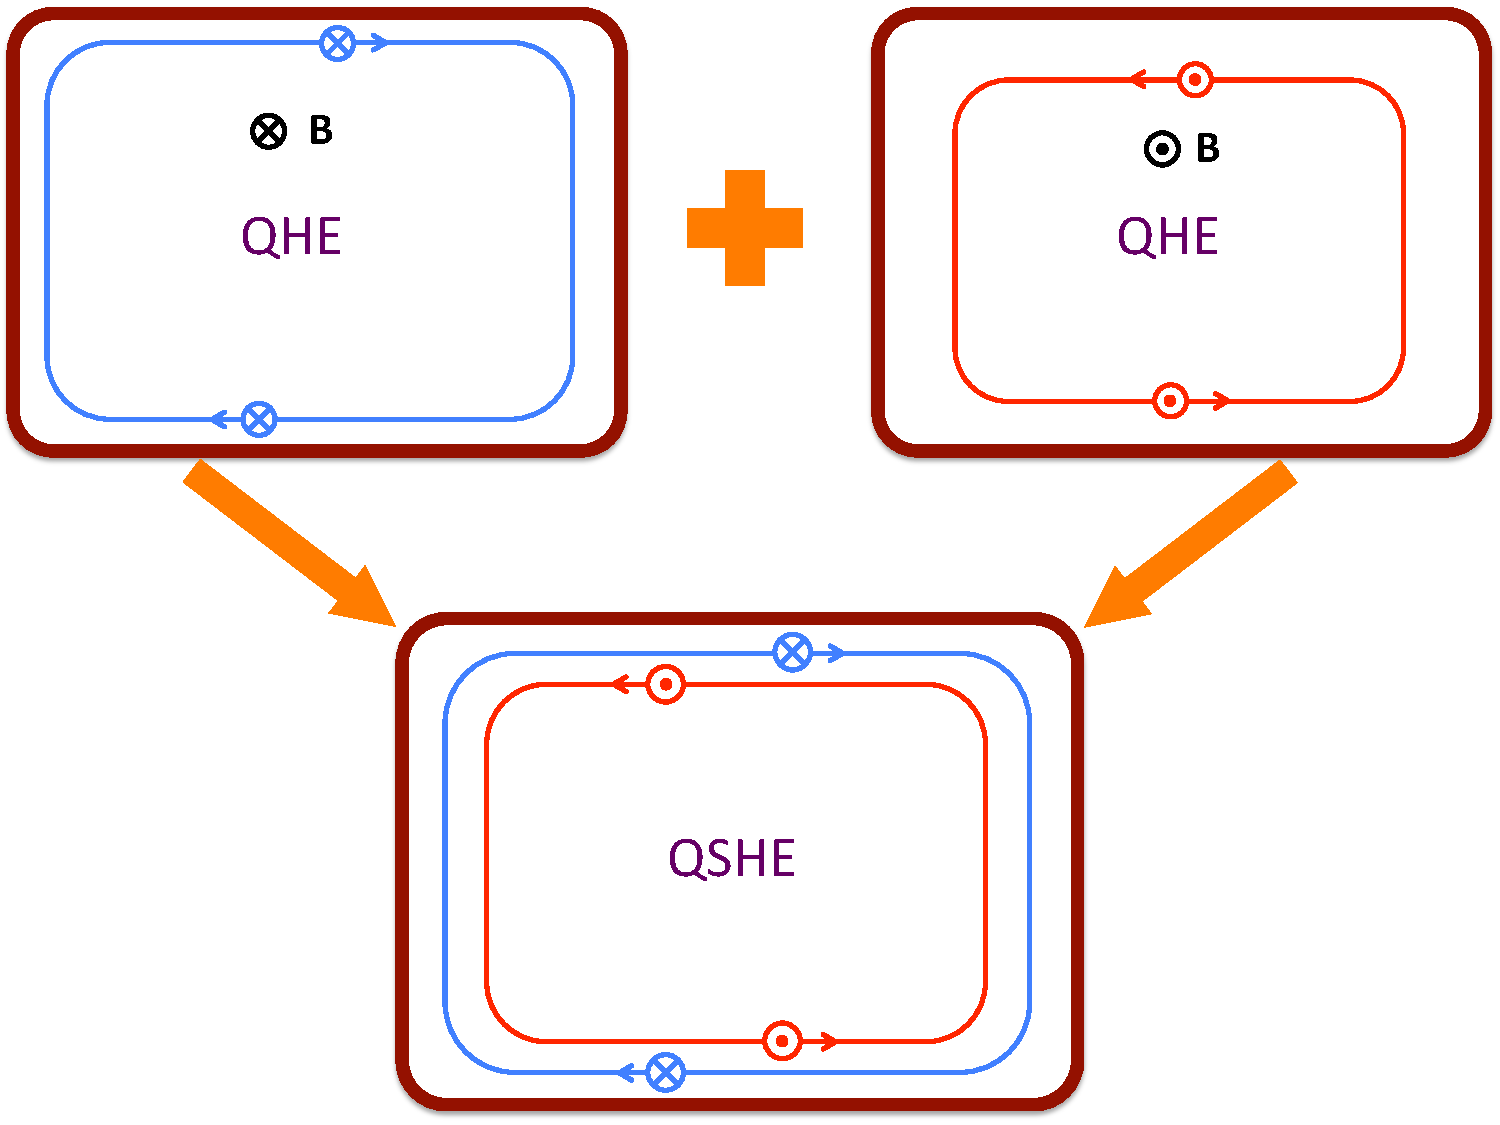
\includegraphics[width=0.9\linewidth]{ch-intro/figures/QSHE.pdf} 
\caption{\label{QSHE} (Color online) 
The edge states in quantum spin Hall effect can be viewed as a stack of two quantum Hall edge states with opposite directions.
} 
  \end{center}
\end{figure}

An important progress later is to extend the topological band theory to the 3D case. In 2007, Fu and Kane~\cite{FuKane07, Fu07} successfully made this step and found the theoretical ingredients for 3D $Z_2$ TIs. They found that four $Z_2$ topological invariants $[\nu_0; \nu_1, \nu_2, \nu_3]$ could be used to classify the different topological properties of a crystal. Within these four numbers, $[\nu_0]$ is the strong topological invariant, which is also the most important one that defines a strong or weak TI. $[\nu_1, \nu_2, \nu_3]$ are called weak topological invariants, and could be used to classify different weak TIs. Fu and Kane~\cite{FuKane07} used the pfaffians at the Kramers points inside the first Brillouin zone to calculate $[\nu_0]$ as the following:
\be
(-1)^{\nu_0}=\prod \delta_a, 
\label{eq:nu0}
\ee
where $\delta_a = Pf[\omega(\Lambda_a)]/\sqrt{Det[\omega(\Lambda_a)]} = \pm1$. Here $Pf[\omega(\Lambda_a)]$ is the pfaffian, and the $
\omega$ matrix is $\omega_{mn}(\bf k) = \Braket{u_{m -k}|\Theta|u_{nk}}$, where $\Theta$ is the time reverse operator. As a result, a 
conventional trivial insulator has topological invariants $[\nu_0; \nu_1, \nu_2, \nu_3] = [0, 0, 0, 0]$. For a strong TI, $\nu_0=1$. A weak TI has $\nu_0=0$ but at least one of the weak topological invariants is non-zero.

\begin{figure}[htb]
  \begin{center}            
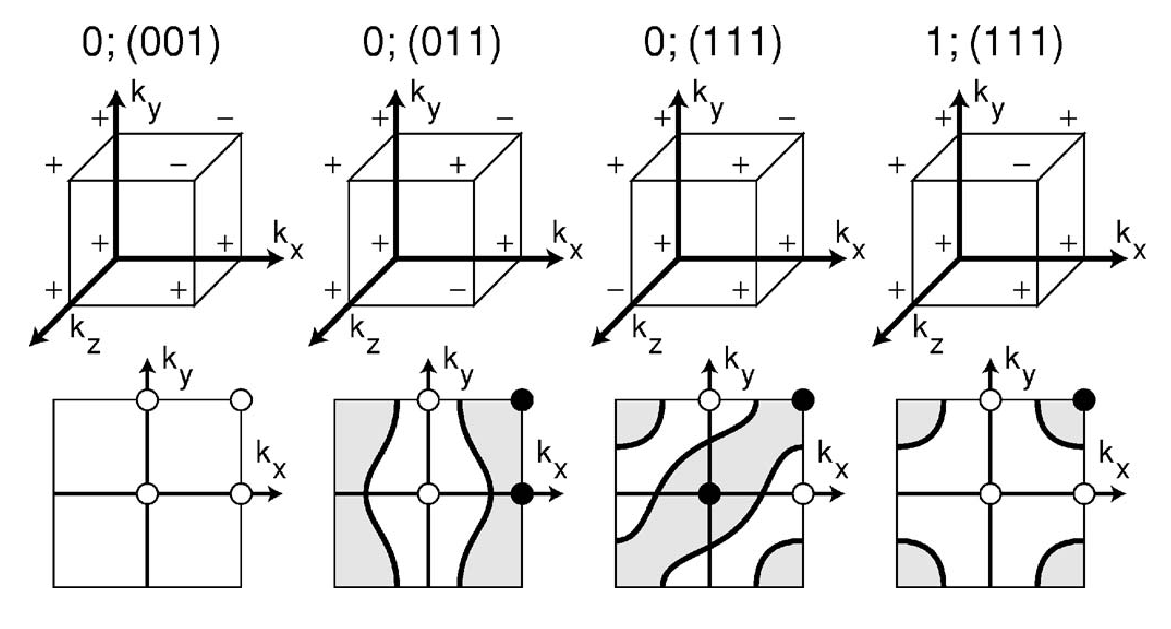
\includegraphics[width=0.9\linewidth]{ch-intro/figures/TI_class.pdf} 
\caption{\label{TI_class} (Color online) 
The four diagrams give examples of different types of weak and strong TIs. The top panels depict the signs of $\delta_i$ at the Cramers points $\Lambda_i$ in the reciprocal lattice. The bottom panels display the corresponding surface states.
} 
  \end{center}
\end{figure}

Same as the earlier found topological phases, a 3D TI also has metallic states on its edge, the 2D surface, while its 3D bulk is an insulator. These surface states also provide an easy way to distinguish strong TIs, weak TIs and trivial insulators in experiments. Fu and Kane pointed out that on the surface of a strong TI, there is an odd number of states connecting the bulk conduction band and the valence band. These surface states, which exist on every plane cleaved out of the crystal, are robust because they cannot be destroyed by local perturbations from the impurities. However, weak TIs only have some robust surface states on certain cleavage planes. By contrast, a trivial insulator do not have such robust surface states at all. Besides, one important property of the surface states on a strong TI is the spin-orbit lock-in effect. Thus, the spin direction of the surface state is always perpendicular to both the wavevector $\bf k$ and the surface normal vector $\bf{\hat{n}}$.

The prediction of the spin-polarized surface states on 3D TI has largely expanded the scope of possible experiments on the topological properties of solids. Most of the experiments are focused on strong TI, and there has been important progress in experiments with techniques like angle-resolved photoemission spectroscopy (ARPES), scanning tunneling microscopy (STM) and transport measurement. The first experimental discovery of a 3D TI is the ARPES result on Bi$_{1-x}$Sb$_x$ by Hasan's group \cite{Hsieh08, Hsieh09}. As shown in Fig. \ref{ARPES_STM}A, there are five surface bands inside the bulk band gap. The spin ARPES data showed that these surface states indeed are spin-polarized. Then more ARPES experiments found that Bi$_2$Se$_3$ and Bi$_2$Te$_3$ \cite{Xia09, Chen09} are also strong TIs but they have a much simpler surface band structure. As shown in Fig. \ref{ARPES_STM}B and D, both Bi$_2$Se$_3$ and Bi$_2$Te$_3$ only have one surface state across the bulk band gap. Since these surface states have a linear dispersion to the first order, they could be described by the Dirac equation and are also called Dirac surface states. They are also a good analog to the Dirac states in graphene. STM experients by Yazdani group\cite{Pedram09} have also confirmed the lack of back-scattering of the topological surface states. 

\begin{figure}[htb]
  \begin{center}            
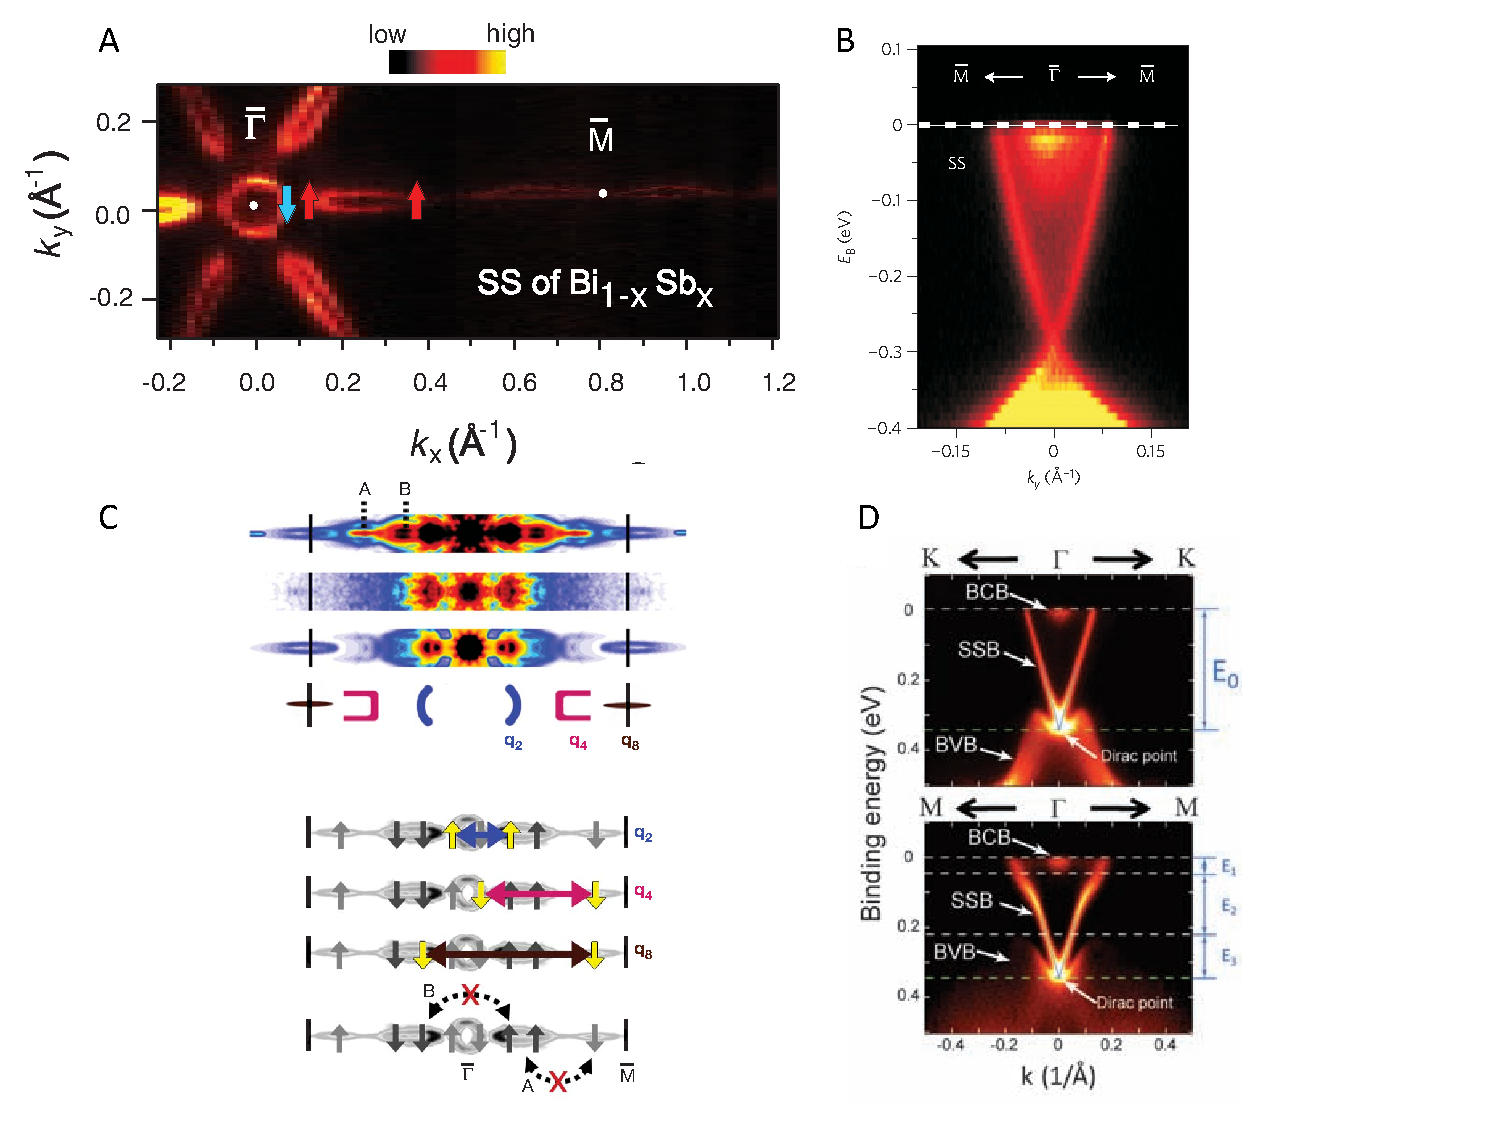
\includegraphics[width=0.9\linewidth]{ch-intro/figures/ARPES_STM.pdf} 
\caption{\label{ARPES_STM} (Color online) 
The first ARPES and STM results on some topological insulators. (A) The ARPES experiment on the first example of a strong TI, Bi$_{1-x}$Sb$_x$, indicates five spin-polarized surface states at the Fermi level\cite{Hsieh09}. (B) The ARPES data on Bi$_2$Se$_3$ shows a single surface cone with a 0.3 eV bulk energy gap \cite{Xia09}.  (C) The quasiparticle interference results in an STM experiment on Bi$_{1-x}$Sb$_x$ confirms the lack of back-scattering of the topological surface states. (D) The ARPES data on Bi$_2$Te$_3$ gives another example of a TI with a single surface cone and a large bulk energy gap \cite{Chen09}.
} 
  \end{center}
\end{figure}

Despite the fast advances in experiments using surface-sensitive techniques, the transport measurement of a TI's surface states have been difficult, mainly due to the vast amount of carriers in the bulk. Unexpected by the theory, the inverted bulk band gap induced by the SOC in TIs may still have a lot of states inside. The reason is that the crystal defects and imperfection in real TI crystals can easily dope the materials and make the as-grown crystals $n$-type (Bi$_2$Se$_3$) or $p$-type (Bi$_2$Te$_3$). Besides, the surface states are still vulnerable possibly due to the chemical reaction that happens when the sample is exposed to air. Hence, the surface states typically contribute only to a small portion of the total current, and thus are hard to detect in transport experiments. Despite the difficulty, Qu et. al. ~\cite{Qu} and Analytis et. al. ~\cite{Analytis} found the first convincing transport signals for the surface states on TI in Bi$_2$Te$_3$ and (Bi$_{1-x}$Sb$_x$)$_2$Se$_3$. These experiments have triggered enormous interest in the transport experiments on TIs. And we will discuss our progress in the transport investigation of TIs in later chapters. 

\begin{figure}[htb]
  \begin{center}            
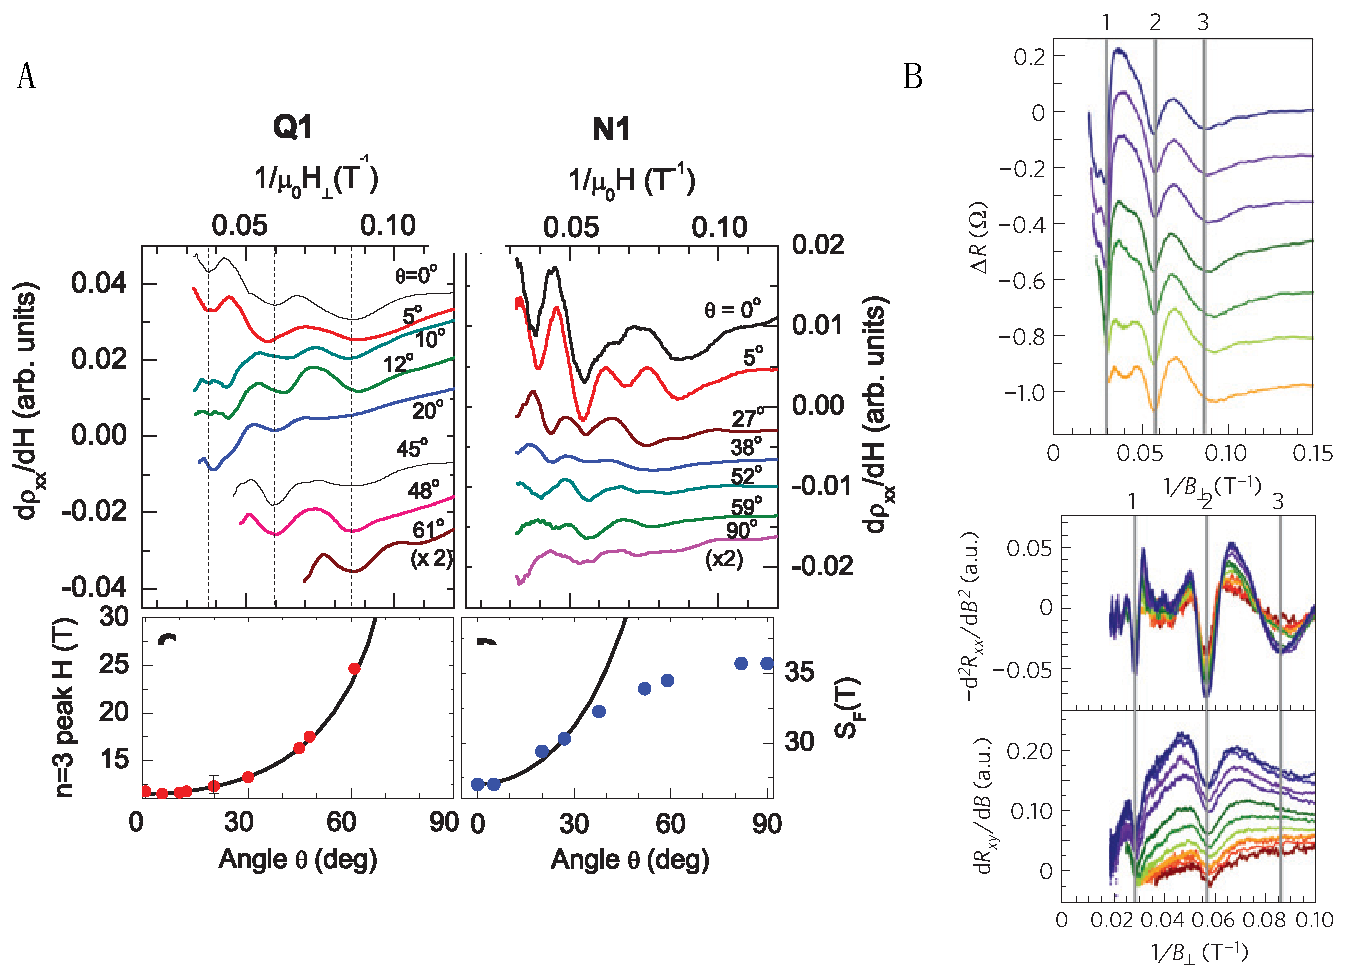
\includegraphics[width=0.9\linewidth]{ch-intro/figures/TI_transport.pdf} 
\caption{\label{TI_transport} (Color online) 
Quantum oscillations at high magnetic fields confirm the existence of high-mobility surface states on TI. (A) The different angle dependences of the quantum oscillations in nonmetallic and metallic Bi$_2$Te$_3$ samples indicate the surface origin of the quantum oscillations in nonmetallic samples. (B) Quantum oscillations in the magnetoresistance data of (Bi$_{1-x}$Sb$_x$)$_2$Se$_3$ are consistent with the behavior of surface states when the magnetic field is tilted.
} 
  \end{center}
\end{figure}



\section{Weyl and 3D Dirac Semimetals}
\label{sec:intro:Weyl}
%1 chiral
%2 from Berry phase to chiral charge
%3 current between the Weyl nodes
%4 poor man�s approach for chiral pumping
%
%experimental progress, ARPES (including Fermi arcs), transport
%
%
%
%Besides the progress in TI, interesting concepts of Weyl semimetals and 3D Dirac semimetals have also been developed.

While the surface states on TI provide an analog to the 2D Dirac electrons in graphene, interesting concepts of Weyl semimetals and 3D Dirac semimetals were also developed as examples of 3D Dirac electrons. With a linear energy-momentum dispersion, both Weyl semimetals and Dirac semimetals can be viewed as 3D analogs of the 2D graphene. Besides, Weyl semimetals provide a solid-state realization of the Weyl fermions that have been studied theoretically for a long time in high energy physics. Weyl fermions are a type of massless fermions with handedness, i.e. chirality. The chirality describes whether a particle spins clockwise or anti-clockwise when viewed in front of the traveling direction. In absence of an electromagnetic field, the chirality of each Weyl fermion is conserved. Therefore, a Weyl fermion cannot shift its handedness without the combination of the electric and magnetic fields. In a 3D crystal, Weyl fermions can be imitated by quasiparticles of electrons with the Hamiltonian as the following:
%\be
%H_{\pm}=\pm \nu_F (p_x \sigma_1 + p_y \sigma_2 + p_z \sigma_3),
%\label{eq:H_W}
%\ee
\be
H=\bf p \cdot \bf V \cdot \pmb{\sigma},
\label{eq:H_W}
\ee
where $\bf V$ is the velocity matrix, $\bf p$ is the electron's 3D momentum vector deduced by the Weyl nodes in the Brillouin zone, and $\pmb{\sigma} = (\sigma_x, \sigma_y, \sigma_z)^T$ denotes the vector formed by the three Pauli matrices. If a Weyl node is at $\bf{k_W}$ in the reciprocal space, then $\bf p= \hbar (\bf k-\bf k_W)$, where $\bf k$ is the electron's wavevector. The Pauli matrices $\sigma_i$ (i = x, y, z) live in the space spanned by the pair of bands that touch at the Weyl nodes. Here each of the two bands is single-degenerate. Thus the system could not respect time reversal and inversion symmetry simultaneously. The above equation shows that the chirality in the Weyl semimetal is formed by the electron's momentum and its peudospin described by the Pauli matrices. Then the chirality of the system is $\chi = sign(det(\bf V))$, which could be $\pm 1$ for the left-handed and right-handed Weyl fermions respectively. As in the case of high-energy Weyl fermions, the Weyl nodes in a crystal always appear in pairs with opposite chiralities. The crystal whose low energy dispersion could be described by Eq.\ref{eq:H_W} near a Weyl node is called a Weyl semimetal.

In addition, we may also have a pictorial understanding of the Weyl nodes and their chiralities from the perspective of the Berry phase. A Bloch 
electron moving inside the Brillouin zone feels the Berry vector potential $\bf A(\bf k) = i \Bra{u(\bf k)}\bf \nabla_{\bf k} \Ket{u(\bf k)}$. This vector potential yields the Berry field $\bf F(\bf k)=\bf \nabla_{\bf k} \times \bf A(\bf k)$ that deflects the direction of Bloch electrons in the momentum 
space. $\bf F(\bf k)$ is also called the Berry curvature or the Chern flux. Thus $\bf F(\bf k)$ acts as a magnetic field that bends the momentum trajectory of a moving electron in a crystal. In a WSM, the chirality $\chi$ of a Weyl node can be calculated by the total Berry flux through an enclosing surface with the following equation:
\be
\frac{1}{2\pi}\oiint\limits_{FS} \VF{F(k)} \cdot \dif{\VF{S(k)}}=\chi, 
\label{eq:chi_Berry}
\ee
where the integral is over the whole Fermi surface that encloses the Weyl node. This equation suggests that a Weyl node acts as a monopole that generates the Berry curvature in the momentum space. Weyl nodes with opposite chiralities are similar to magnetic monopoles with opposite magnetic charges. Besides, since $\bf F(\bf k)$ is the Chern curvature, the above equation indicates that a Fermi pocket that encompasses a Weyl node has a non-trivial Chern number $\chi$.

In a crystal with both time reversal symmetry and inversion symmetry, such separated Weyl pairs do not exist because the bands involved are always degenerate. When two Weyl nodes with opposite chiralities meet in a crystal, they generally annihilate and open a band gap. However, Wang et. al.~\cite{Wang2012, Wang2013}  found that with certain crystal symmetries, paired Weyl nodes can overlap in the momentum space and it results in a new crystal with a linear energy-momentum dispersion, namely a 3D Dirac semimetal. Unlike a WSM, a 3D Dirac crystal respects time reversal and inversion symmetries at the same time. Besides, 3D Dirac cones also accidentally exist in many solids. For example, at the phase transition between a topological insulator and a trivial insulator, the conduction and valence bands of the crystal touch and form a linearly dispersed Dirac cone. However, such accidentally formed Dirac semimetals are not stable since they need fine tuning of chemical compositions and a small perturbation may open a gap at the Dirac point. Nevertheless, the DSMs found by Wang et. al. ~\cite{Wang2012, Wang2013}, i.e. Cd$_3$As$_2$ and Na$_3$Bi, are robust against small perturbations due to the protection by the crystal symmetries. Wang et. al. also predicted the existence of the surface Fermi arcs that connect different Dirac points. Their predictions have been confirmed by ARPES experiments~\cite{Liu2014a, Xu2015, Liu2014, Neupane2014}. Thus such crystals become the maternal materials for Weyl semimetals. Later, Weng et. al. ~\cite{Weng2015} and Huang et. al. group ~\cite{Huang2015} predicted a series of Weyl semimetals that lack inversion symmetry, such as TaAs and NbAs. In these crystals, the Weyl nodes are already separated due to the lack of the inversion symmetry. They also predicted Fermi arcs on the surface that connect the bulk Weyl nodes.Then these findings were confirmed by ARPES experiments~\cite{Xu2015}.

Besides the value in the theoretical aspect, Weyl semimetals also have very interesting transport properties. One of them is the chiral anomaly effect that pumps charges from one Weyl branch to its pair in the presence of an electromagnetic field. A simple picture to understand the chiral anomaly effect in a Weyl semimetal is as the following. If we suppose that the Weyl fermion has entered the lowest Landau level (LL) in a strong magnetic field. The energy dispersion for the $n=0$ Landau level is $\varepsilon_0 = -\chi \hbar \nu_F \VF{k \cdot \hat B}$, where $\hbar$ is the Planck constant and $\VF {\hat B}$ is the normal vector of the magnetic field. We suppose that both the temperature and the chemical potential are low (smaller than $\nu_F \sqrt{\hbar eB}$). Also, the degeneracy of one Landau level formed by one Weyl node is $g = \frac{B S}{h/e}$, where $S$ is the cross-section of the sample that is perpendicular to $\bf B$. If an electric field $\bf E$ is also applied on the same direction as $\bf B$, the states in the momentum space will move according to $\hbar \VF{\dot{k}}=-e  \VF{E}$. Thus the charge pumping rate between Weyl nodes with opposite chiralities is $\VF{\dot{Q}} = e \chi g L |\VF{\dot{k}}|/2\pi=-e^2 \chi g L|\VF{E}|/h$, where L is the length of the crystal along the $\bf B$ direction. Putting in the expression for the degeneracy of the lowest Landau level, we obtain the charge pumping rate for unit volume:
\be
\VF{\dot{Q}}= -\frac{e^3}{4\pi^2\hbar^2} \VF{E} \cdot \VF{B}
\label{eq:chg_pmp}
\ee

%Although we only showed the correctness of the above formula in the case of the lowest LL and when $\bf B$ and $\bf E$ are parallel, strict calculations (cite) have shown that this formula is concrete even more LLs are occupied when $\bf B$ and $\bf E$ are not parallel. 

Although it seems to annhilate or create charges for one Weyl branch, the pumping effect does not violate the charge conservation law in a crystal because Weyl nodes with opposite chiralities always appear in pairs. The above charge pumping effect is also called Adler-Bell-Jackiw chiral anomaly, which was originally used to explain the neutral pion decay in particle physics. Thus the WSM provides us an opportunity to study the chiral anomaly phenomenon in high energy physics.

\begin{figure}[!htbp]
  \begin{center}            
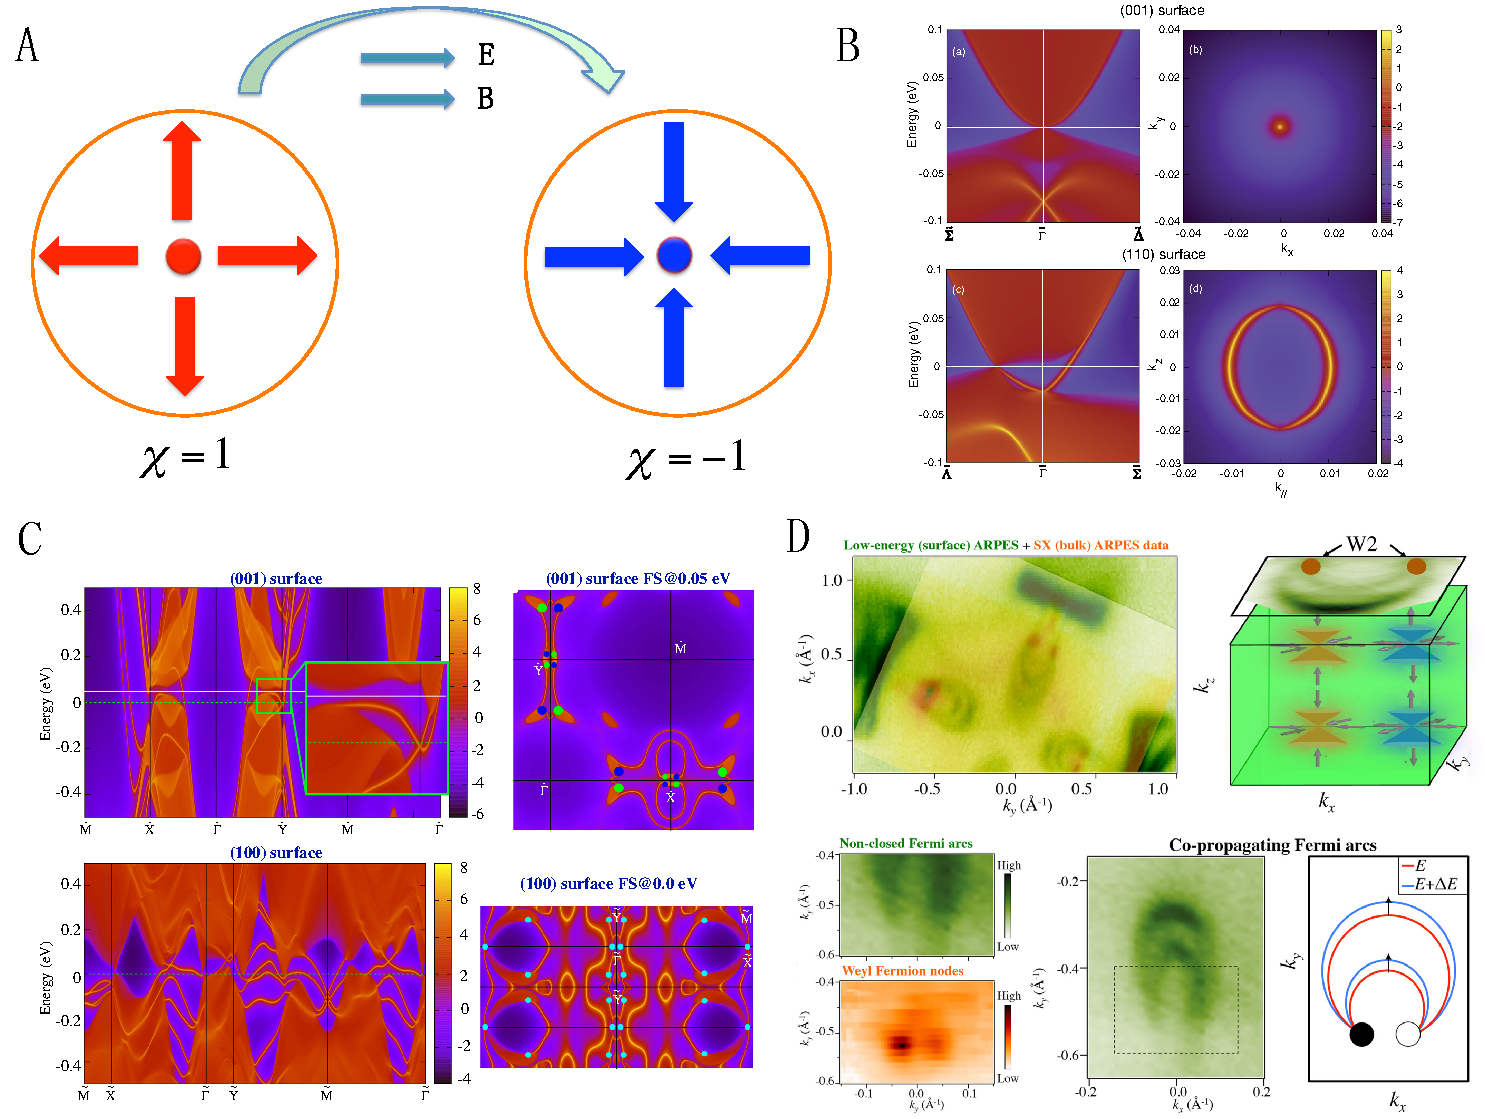
\includegraphics[width=0.9\linewidth]{ch-intro/figures/WeylDirac.pdf} 
\caption{\label{QSHE}
The Weyl and Dirac nodes of Weyl semimetals and Dirac semimetals. (A) The paired Weyl nodes are opposite monopoles of the Berry curvature. In an electric-magnetic field, charges are pumped between the Weyl nodes. (B) The predicted Dirac node and surface Fermi arcs of the Dirac semimetal Cd$_3$As$_2$~\cite{Wang2013}. (C) The predicted multiple Weyl nodes and the surface Fermi arcs that connect them in the Weyl semimetal TaAs~\cite{Weng2015}. (D) ARPES experiments by Hasan's group confirmed the surface Fermi arcs on TaAs~\cite{Xu_TaAs}.
} 
  \end{center}
\end{figure}



\chapter{Experimental Setup\label{ch:expsetup}}

In this chapter, we will briefly discuss some details of the transport techniques we use in our study of the topological insulators and Dirac semimetals. The research work in this thesis heavily depends on the magnetoresistance data at low temperatures. Hence I will first introduce the systems we use for our magnetoresistance and Hall measurement. Besides, we have developed the ionic liquid gating technique to tune the chemical potential in the TI experiments. Ionic liquid turns out to be a powerful dielectric material for gating semiconductors with a flat surface, such as TIs. But it also takes a large amount of effort to avoid chemical contamination and to obtain strong and robust results from the ionic liquid gating method. We will discuss our ways of using the ionic liquid on TIs. At the end of this chapter, we will introduce our method to protect and measure the air-sensitive Na$_3$Bi crystals. As we discussed in the previous chapter, Na$_3$Bi has two 3D Dirac nodes inside, and serves as a platform to study the long-sought Weyl physics. Unfortunately, due to the strong metallicity of Na atoms, Na$_3$Bi crystals are prone to oxidization by any amount of oxygen or water. Therefore, it takes enormous effort to preserve the Na$_3$Bi samples during the contact mounting process and the measurement process.

% include other files for sections of this chapter. These use the 'input' command since each section within a chapter should not start a new page.
% If you want to swap the order of sections, it is as simple as reversing the order you include them. 
\section{Low-Temperature Transport Measurements in a Strong Magnetic Field}
\label{sec:expsetup:magnet}

\subsection{High Field Magnets and Cryostats}\label{magnet}

The main in-house magnets we use are the 14 Tesla superconducting magnet from Oxford Instruments, the 15 Tesla superconducting magnet from American Magnetics, and the 9 Tesla Physical Property Measurement System (PPMS) from Quantum Design. Besides, we also use the 35 Tesla Resistive Magnet, the 45 Tesla Hybrid Magnet, and the 65 Tesla Pulse Field Magnet at National High Magnetic Field Laboratory (NHMFL) to study our samples at high fields. The high field data can provide us important information such as low Landau levels and possible new phases.


\begin{figure}[!htbp]
  \begin{center}
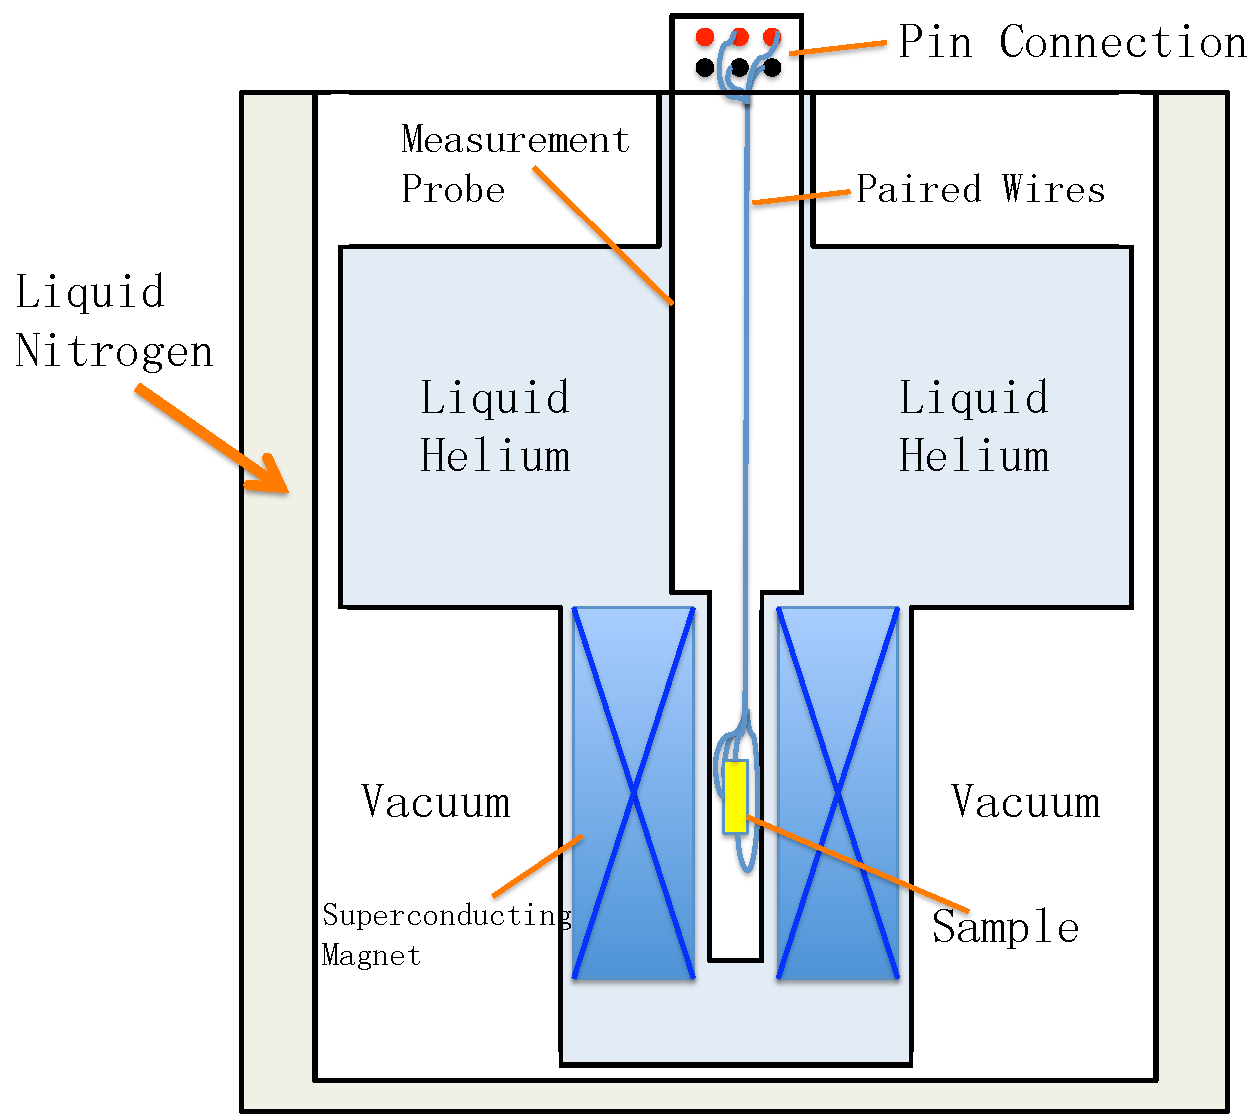
\includegraphics[width=0.8\linewidth]{ch-expsetup/figures/Magnet14T.pdf}
\caption{\label{Magnet14T}
A sketch of a typical in-house superconducting magnet with a measurement probe inside.}
  \end{center}
\end{figure}

Our in-house magnets are similar in their structures as shown in Fig. \ref{Magnet14T}. Each magnet has a dense coil made out of superconducting materials. The coil, with a bore for the measurement probe, is immersed by liquid helium in a dewar with a vacuum jacket. Outside the vacuum jacket, there is a liquid nitrogen jacket in order to reduce the thermal radiation from the helium container. The coil has a critical temperature higher than 4.2 K, and thus the coil will stay in the superconducting state when the current is flowing inside. The current is driven by an outside power supply. 

\subsection{Transport Measurement}\label{transport}

%talk about Sample Sample method
To make ohmic contacts to the samples, we typically use the silver paint from Dupont and thin gold wires to connect the sample to the measurement pads on the sample stage. To measure the magnetoresistance at tilted magnetic fields, we leverage our home-made rotation probe and the rotation probe that accompanies PPMS to rotate the sample in a magnetic field. Our home-made rotation probe has a Hall probe to tell the angle relative to the direction of the magnetic field. It can reach a temperature as low as 4.5 K, while PPMS's rotation probe can get to 2 K. To measure the transport property below 4 K, we use the He3 inserts from Oxford, Janis and IceOxford to to attain 0.3 K. Besides, NHMFL provides measurement inserts for both 4K-above and 4K-below transport measurements in the high-field experiments. To stabilize the temperature, we use the Lakeshore 340 temperature controller to adjust the heating power on the sample stage. 

The resistivity transport measurements were accomplished in different ways, such as by the lock-in technique and the delta-mode method. In the PPMS, we use the DC Resistivity mode (which is actually a delta mode) to measure the magnetoresistance. To measure the sample resistance in our in-house superconducting magnet, we typically use the SR830 Lock-in Amplifier from Stanford Research to implement the lock-in measurement, or use Keithley's 6221 current source and 2182A nano voltmeter for the delta-mode method. The choice depends on the sample's resistance as well as its contact resistance. Besides, the current through the sample is carefully chosen so that it has a large signal-to-noise ratio and does not increase the sample temperature. 

The Hall measurement is conducted in a way similar to the resistance measurement. But one noticeable detail is the method to measure the temperature dependence of the Hall coefficient. Here we implement the reciprocal technique set up by Sample et.al.\cite{Sample1987}. This method leverages the reciprocal theorem in electrodynamics so that the magnetic field does not need to be flipped during the Hall measurement. 

The main idea in Sample's work\cite{Sample1987} is as the following. Suppose there is a sample with four contact leads labeled as 1, 2, 3 and 4 respectively. In a magnetic field pointing to the positive direction, we first measure the resistance $R_{12, 34} (+B)$ by sending a current through leads 1 and 2, while measuring the voltage on leads 3 and 4. When we reverse the field direction, $R_{34, 12} (-B)$ denotes the resistance measured across the leads 1 and 2 with the current flowing through the leads 3 and 4. And the reciprocal theorem gives $R_{12, 34} (+B) = R_{34, 12} (-B)$. Therefore, we can also obtain $R_{12, 34} (-B) = R_{34, 12} (+B)$. In a Hall measurement, we normally need both $R_{12, 34} (+B)$ and $R_{12, 34} (-B)$ to calculate the Hall signal by $R_{yx} (B) = (R_{12, 34} (+B) - R_{12, 34} (-B))/2$ so that the extra contribution from the longitudinal resistance can be neutralized. But this conventional way also requires a change of the field direction, which usually takes a long time. Here we replace $R_{12, 34} (-B)$ with $R_{34, 12} (+B)$, and obtain $R_{yx} (B) = (R_{12, 34} (+B) - R_{34, 12} (+B))/2$. As a result, we do not need to flip the magnetic field. Instead, we need to switch the current and voltage leads, which can be done quickly with an electric relay switch. Using this method, we are able to switch the the current and voltage leads at each temperature and then measure the Hall coefficient v.s. temperature curve in a short time. 

\section{Ionic Liquid Gating Technique}
\label{sec:expsetup:ionicliquid}

Ionic liquid gating technique is a novel gating approach. Similar to the traditional solid gating method, ionic liquid gating also leverages a thin capacitor to change the chemical potential on the surface of a sample. One plate of the capacitance is also the sample surface. But unlike the solid state gating, the other capacitance plate is one layer of ions in the ionic liquid. Besides, since the ions sit on top of the sample surface, the thickness of the capacitor is on the order of the atomic scale. Thus it provides a very large capacitance and leads to a powerful gating effect. Previously, Iwasa's group first demonstrated the power of ionic liquid on ZnO\cite{yuan2009ZnO}. Then together with Iwasa\cite{Yuan2011}, Ando \cite{Ando_liquid} and Tokura group\cite{Checkelsky_liquid}, we introduced this novel gating method into TI transport experiments\cite{Xiong2013}. We discuss some technical details of the ionic liquid gating experiments here. 

The ionic liquid we use is DEME-TFSI, comprised of cations (CH$_3$ CH$_2$ )$_2$ (CH$_2$ CH$_2$ OCH$_3$ )CH$_3$ N$^+$ and anions (CF$_3$SO$_2$)$_2$N$_-$. This ionic liquid has been proved to provide a powerful gating effect in previous experiments\cite{yuan2009ZnO, ye2010liquid}. Before using the liquid, we pump it at $25 \,^{\circ}{\rm C}$ for 2 hours in order to minimize any water content that can accelerate unfavorable chemical reactions. Then the sample, the ionic liquid and the gold gate plate are put into a sapphire container (as shown in Fig. \ref{ILcontain}), and are quickly loaded into the cryostat. Then the sample is fast cooled down to around 220 K to diminish any chemical reaction or damage that may happen to the sample before the liquid freezes. As displayed by Fig. \ref{ILcontain}, there is a gold plate at the bottom of the container that serves as the gate electrode. Above the ionic liquid melting temperature, when a gate voltage is applied between the sample and the gold plate, ions will move inside the liquid. If the gate voltage $V_G$ is positive, cations will drift away from the gate plate and come to the sample surface, while anions will leave the sample. As a result, there forms a thin layer of extra cations on the sample surface, and these ions will generate a strong electric field towards the sample and lift its chemical potential. 

Starting from 0 V, we then apply a gate voltage $V_G$ to the gold plate at a �gating temperature� around 220 K at a sweeping speed of approximately 1 V/min. After the planned $V_G$ is attained, the sample is quickly cooled to 160 K to reduce the possibility of chemical reactions. Then the sample and the liquid are cooled down to 4 K slowly (at 2 K/min) to reduce the stress on the sample and the contacts caused by the freezing ionic liquid. The cooling process has a possibility to damage the sample as we find that repeated freezing and thawing of the ionic liquid can snap the leads or the crystal itself. At 4 K, the large $E$-field induced by the frozen surface anion density $N_{ion}$ (1-4$\times 10^{14}$ cm$^{-2}$) creates a depletion layer that changes the chemical potential in the sample significantly.

Unfortunately, the large gating power is not free. It is more difficult to change the gating voltage with the ionic liquid than using the solid-state gating. Every time we change $V_G$, we need to slowly (at 2 K/min) warm up the sample to the "gating temperature" around 220 K and change $V_G$ by small steps. At the "gating temperature", a typical way to change $V_G$ is to change it in steps of $\sim$0.02 V every 5 to 10 seconds, while monitoring the transient current $I_{trans}$ (1-40 nA). The time spent at the "gating temperature" is typically 300-500 s. Then the sample is cooled down to 5 K with the gating voltage fixed as we discussed above. To minimize the sample damage, we start at $V_G$ = 0 V during the first cool-down, followed by measurements at increasingly negative $V_G$ until the sample fails (usually by a discharge event).  We emphasize that the changes to the resistivity $\rho$ and the Hall density $n_H$ are reversible (see below) as long as $|V_G|$ does not exceed a limit. Upon returning $V_G$ to 0 V, we could recover the same starting value of R (at 5 K) provided $|V_G|$  is kept below 2 V.

\begin{figure}[!htbp]
  \begin{center}
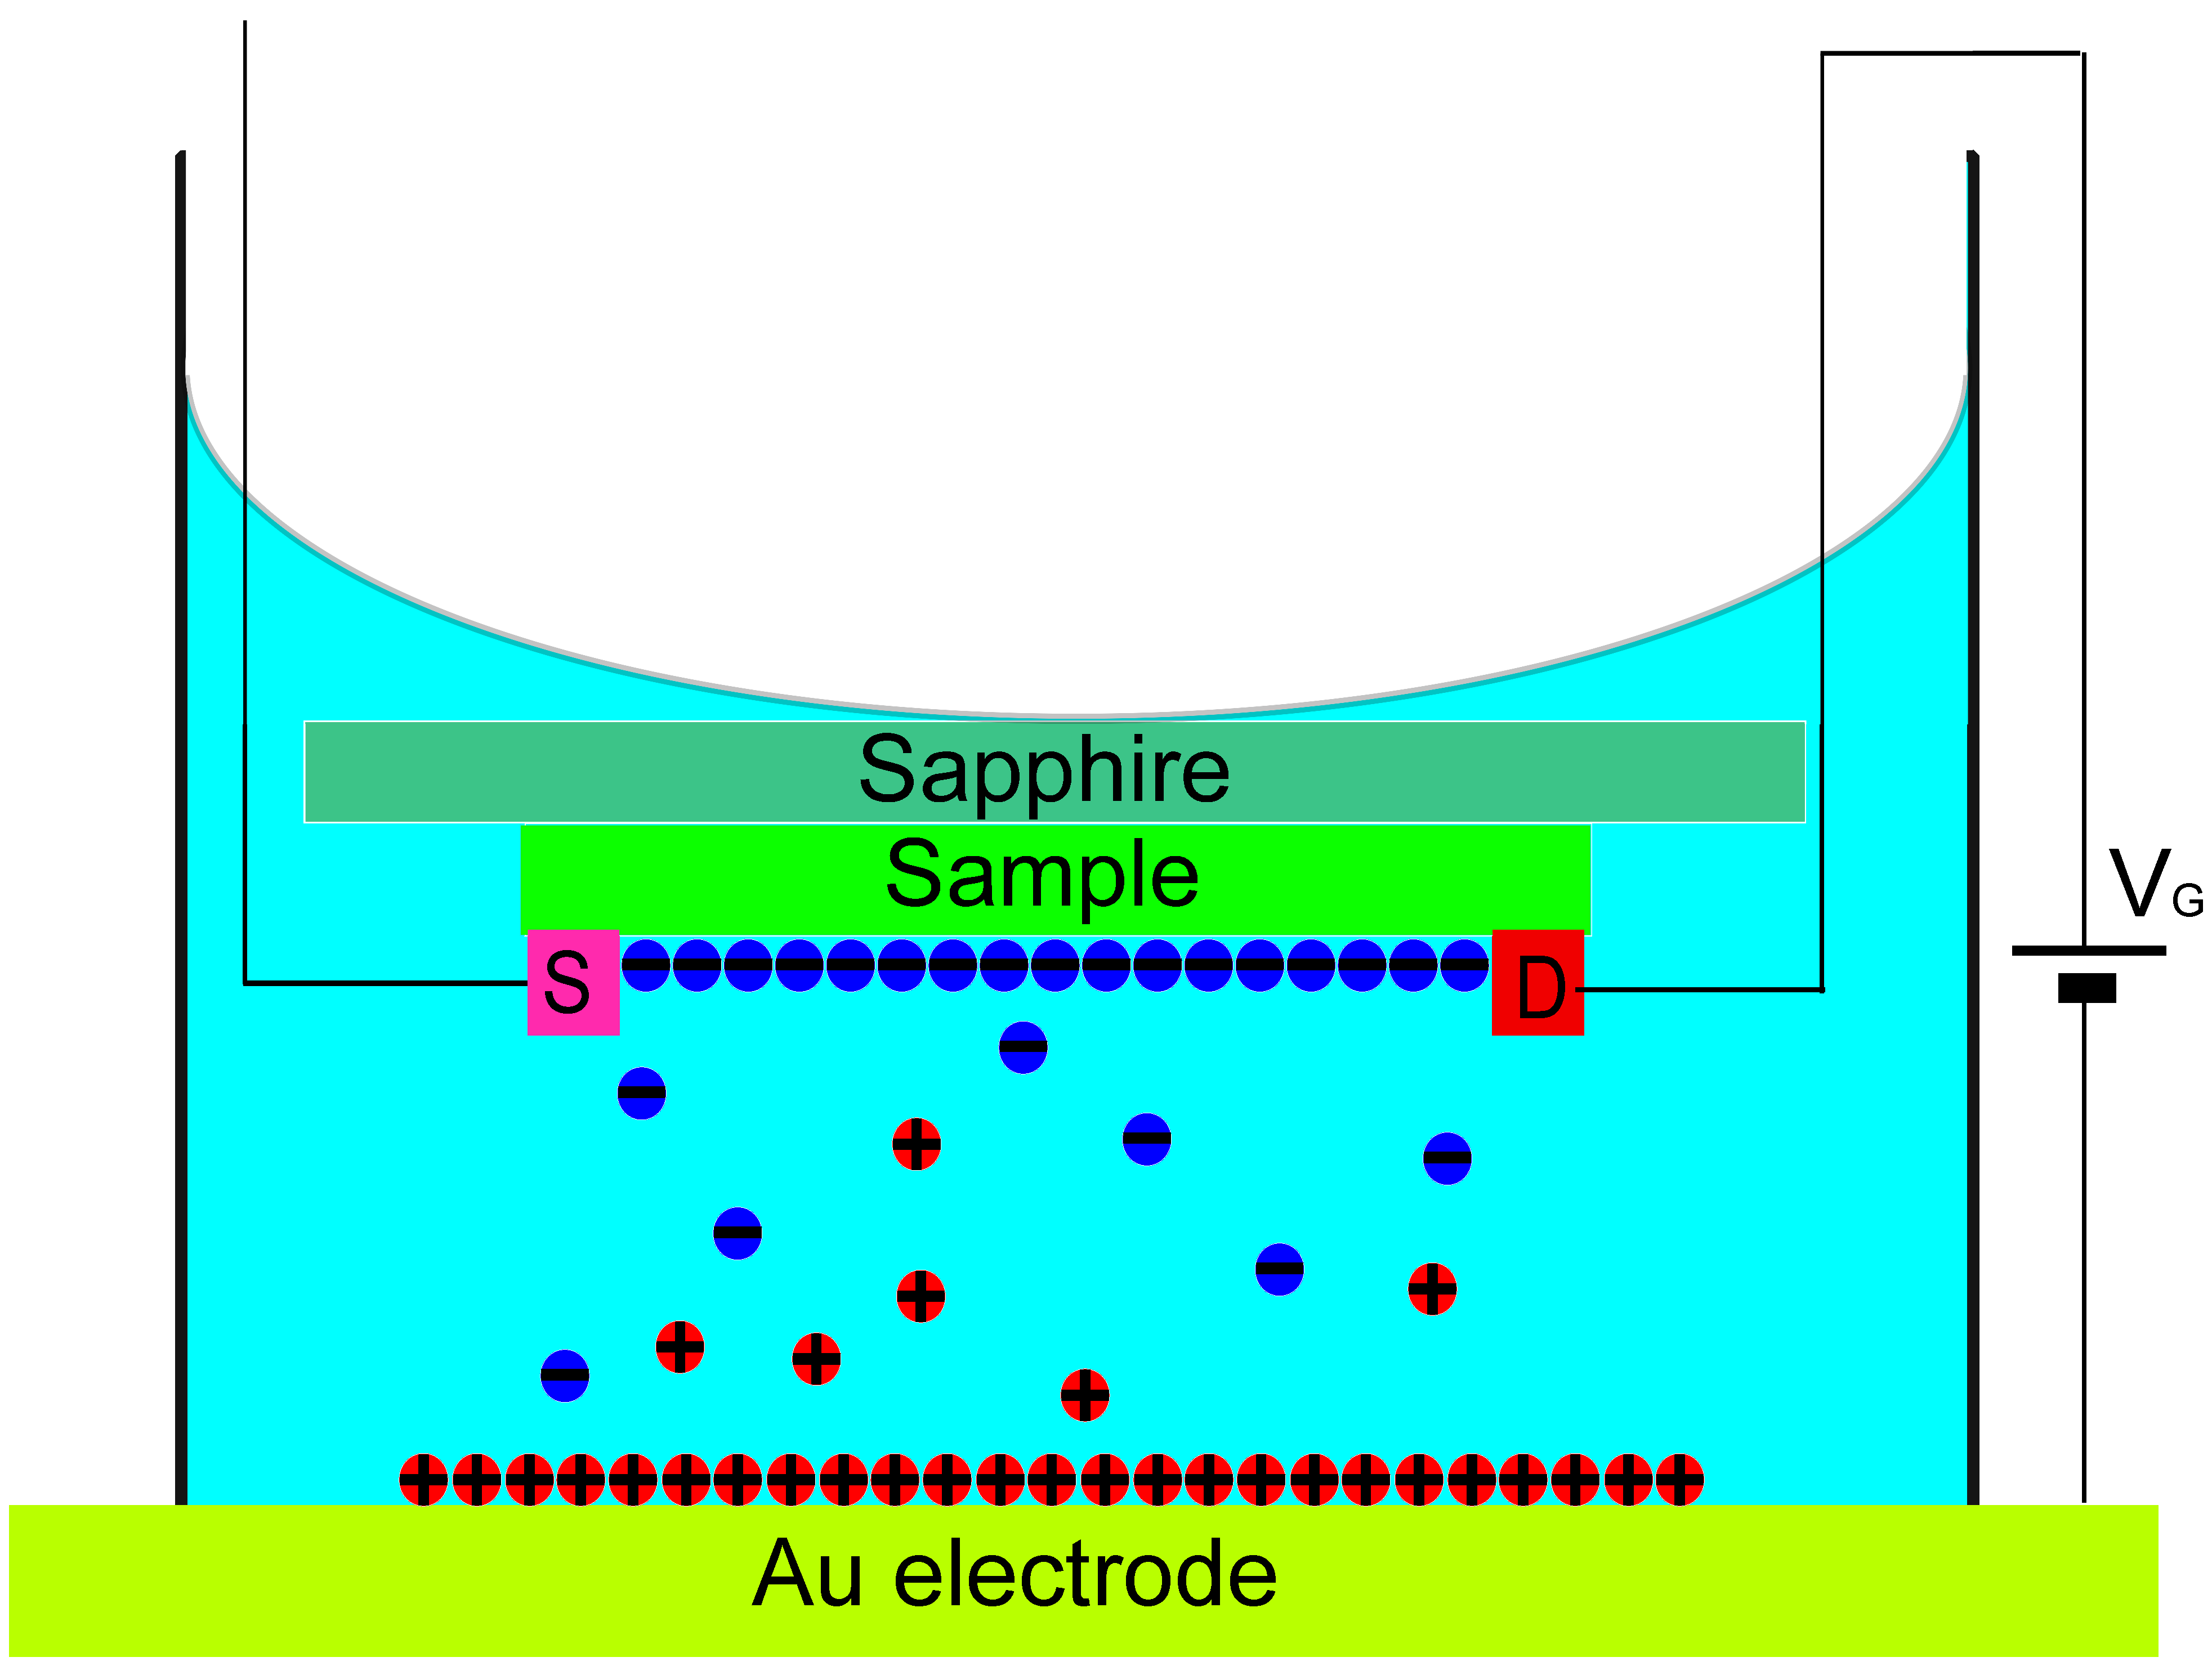
\includegraphics[width=0.8\linewidth]{ch-expsetup/figures/ILcontain.eps}
\caption{\label{ILcontain}
The configuration of the ionic liquid gating experiment. Both the ionic liquid and the sample are held in a sapphire container with a gold plate at the bottom. The Au plate is used to apply a gating voltage to the sample.}
  \end{center}
\end{figure}
\section{Protection of Air-sensitive Samples for Electric Measurement}
\label{sec:expsetup:airsensitive}

The Dirac semimetal Na$_3$Bi is an air-sensitive crystal. Due to the chemical reactivity of sodium, the whole Na$_3$Bi crystal can be easily oxidized in the air within ten seconds. Therefore, we need to make contacts to the sample within the glove box and then seal it well. The sample can only be loaded into the cryostat when it's isolated from any air or water. Great care should be taken during the process. Any remnant oxygen or water in the glove box, or any leaks in the seal can easily turn the crystal into ashes. 

Such fragileness of Na$_3$Bi crystals has created a large obstacle for us to make the electric contacts. To avoid any oxidization, we have to make contacts to the sample in the Argon glove box. Here we use silver epoxy (Epotek H20E) to fix the platinum wires on the crystals. We first put Pt wires and the silver epoxy on the right spot of the samle, then heat it at around 120 $\celsius$ for about 5 minutes so that the silver epoxy matures. Then we put the sample inside a small cylinder container as shown in Fig. \ref{Na3Bi_container} and connect the Pt wires to the electric pads on the cap of the container. We diminish the chance of oxidization by adding paratone oil inside the container after the sample is mounted. Thus the sample is completely immersed in the paratone oil. Then the container is sealed and put into a cryostat for the measurement. Our results show that the sample can survive inside the container for a couple of days even when the container is exposed to air. Once the crystal is loaded into a cryostat and stays below 100 K, the sample stays the same during a long time of measurement. Hence we are able to measure the same Na$_3$Bi sample in different cryostats for a long time.


\begin{figure}[!htbp]
  \begin{center}
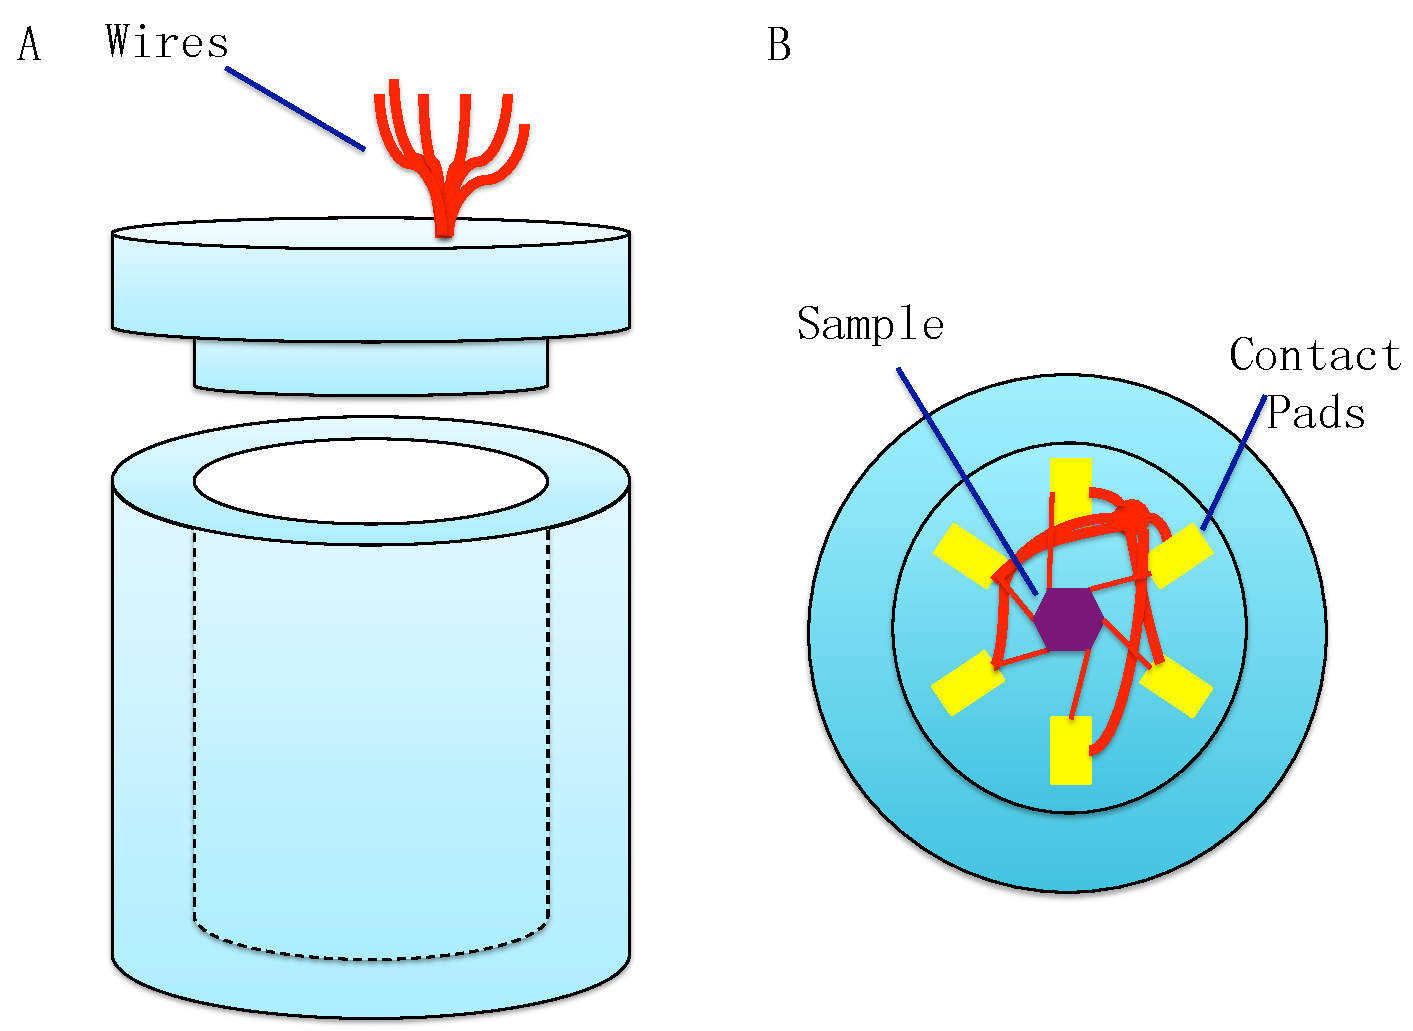
\includegraphics[width=0.8\linewidth]{ch-expsetup/figures/Na3Bi_container.pdf}
\caption{\label{Na3Bi_container}
A sketch of the container that we use to protect the Na$_3$Bi crystal. Panel (A) shows that the container has a bucket and a cap. There are wires  going through the cap. Before the seal, the main bucket is filled with paratone oil to prevent oxidization. Panel (B) shows that the sample is mounted on the inner side of the cap. There are Pt wires connecting the sample and the contact pads on the cap. 
}
  \end{center}
\end{figure}








\chapter{Shubnikov$-$de Haas oscillations in Bi$_2$Te$_2$Se\label{ch:bts}}

Although topological insulators are supposed to have an insulating bulk that does not conduct, previous transport experiments on the suggested TIs found that most of the TI materials have a large bulk conductivity due to the crystal defects and imperfection. For example, although Bi$_2$Se$_3$ and Bi$_2$Te$_3$ have a simple surface state and a large band gap (on the order of 0.3 eV), their bulk carrier densities can only be reduced to approximate $10^{18} cm^{-3}$ after a large amount of work. Furthermore, the chemical doping method that is used to reduce the carrier densities in Bi$_2$Se$_3$ and Bi$_2$Te$_3$ is likely to reduce to the surface mobility. As a result, the surface current is hard to detect and easily immersed in the overwhelming bulk current. The bulk carriers are usually caused by the intrinsic imperfection of the crystals. For instance, despite of extra Se pressure in the growing environment, a large number of Se vacancies can still be generated in Bi$_2$Se$_3$ and then lead to n-type carriers in the as-grown crystals. Meanwhile, Bi$_2$Te$_3$ is known to have Bi-Te anti-site defects that produce p-type carriers. 

Consequently, the metallic bulk has been a big obstacle to the study of new transport phenomena on TIs. Although there are many proposed transport experiments to search for novel physics on the surface of TIs, they depend on a high-quality surface current and the high carrier density in the bulk has severely hampered the progress. Therefore, it is important to reduce the bulk carriers in order to investigate the surface states on TIs. 

To overcome the difficulty, we grew various TI crystals to suppress the bulk carrier density. Among these crystals, one of the most promising ones is Bi$_2$Te$_2$Se. Since Bi$_2$Se$_3$ is n-type due to the Se vacancies and Bi$_2$Te$_3$ is p-type due to the Bi-Te anti-sites, we believe the combined Bi$_2$Te$_2$Se could have a charge compensation between the n-type and p-type carriers. As a result, Bi$_2$Te$_2$Se is likely to have much fewer bulk carriers. In addition, since Bi$_2$Te$_2$Se is a stoichiometric crystal, the surface mobility won't be sacrificed by the chemical dopants.

In this section,we will discuss our transport results on Bi$_2$Te$_2$Se, a TI compound with a large bulk resistivity (6 $\Omega$cm at 4 K). We have observed prominent Shubnikov-de Haas (SdH) oscillations in Bi$_2$Te$_2$Se, which could be used to detect the surface states out of the bulk signal. A fitting to the oscillations yields a surface mobility ($\mu_s\sim$ 2,800 cm$^2$/Vs), which is much larger than the bulk mobility ($\mu_b\sim$ 50 cm$^2$/Vs). These parameters indicate a high surface to bulk current ratio in Bi$_2$Te$_2$Se and it has a potential to serve as the platform TI material for searching Majorana fermions and  axion electrodynamics.

% include other files for sections of this chapter. These use the 'input' command since each section within a chapter should not start a new page.
% If you want to swap the order of sections, it is as simple as reversing the order you include them. 
\section{Crystal and Band Structure of Bi$_2$Te$_2$Se}
\label{sec:bts:bts-band}

Bi$_2$Te$_2$Se's crystal structure is similar to Bi$_2$Te$_3$, with a tetradymite structure and a rhombohedral unit cell. Its space group is $R\bar{3}m$. As shown in Fig. \ref{BTS_structure}A, compared with Bi$_2$Te$_3$, the Te layer between two Bi layers in Bi$_2$Te$_2$Se is replaced by one Se layer~\cite{Ando10}. Since the Bi-Se bonds are stronger than the Bi-Te bonds, the Bi atoms are more likely to stay on their sites than to exchange the sites with Te atoms. Thus such a structure may reduce p-type carriers caused by Bi-Te anti-sites. Besides, compared with Bi$_2$Se$_3$, there are no two adjacent Se layers in Bi$_2$Te$_2$Se. The lack of Se-Se bonds in could also reduce Se vacancies as the Se-Se bonds are not strong and may produce Se vacancies. As a result, the crystal structure of Bi$_2$Te$_2$Se may reduce both the n-type and p-type carriers intrinsically. 

\begin{figure}[!htbp]
  \begin{center}            
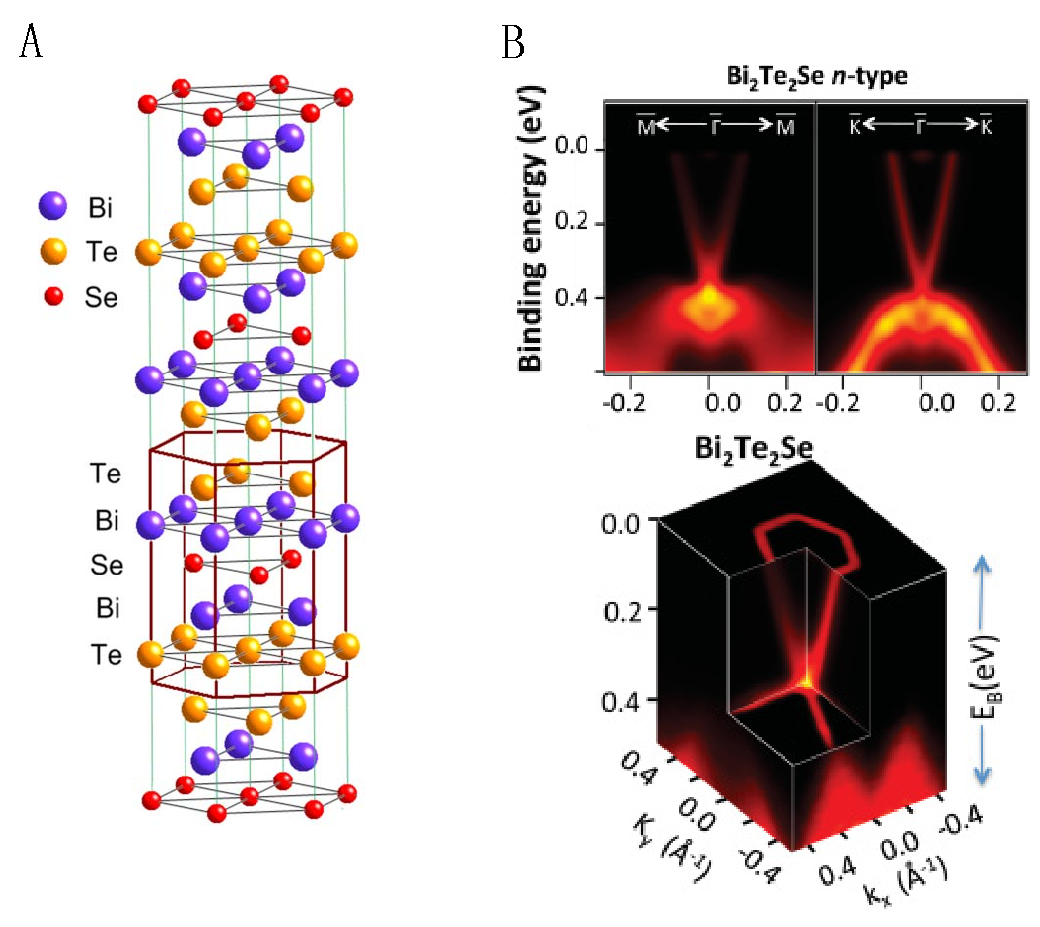
\includegraphics[width=0.9\linewidth]{ch-bts/figures/BTS_structure.pdf} 
\caption{\label{BTS_structure} (Color online) 
The crystal structure and band structure of Bi$_2$Te$_2$Se. (A) The crystal structure of Bi$_2$Te$_2$Se is similar to that of Bi$_2$Te$_3$ with the Te layer between two Bi layers replaced by one Se layer~\cite{Ando10}. (B) The ARPES experiment shows that Bi$_2$Te$_2$Se has a band structure similar to Bi$_2$Te$_3$~\cite{BTS_ARPES}. The band gap is also as large as approximately 0.3 eV, while the surface Dirac point is immersed in the valence band as well.
} 
  \end{center}
\end{figure}

Similar to Bi$_2$Se$_3$ and Bi$_2$Te$_3$, Bi$_2$Te$_2$Se's strong spin-orbital coupling inverts its bulk bands as well. Fig. \ref{BTS_structure}B is the ARPES data on Bi$_2$Te$_2$Se by Hasan's group~\cite{BTS_ARPES}. It demonstrates a clear bulk band gap of approximately 0.3 eV. The V-shape state in Fig. \ref{BTS_structure}B is the spin-polarized single surface Dirac cone. The Dirac point of the surface states is buried in the valence band, as in the case of Bi$_2$Te$_3$.
\section{Experimental Results in the 14T Magnetic Field}
\label{sec:bts:result14T}





%%%%%%%%%%%%%%%%%%%%%%%%%%%%%%%%%%%%%%%%
%%%%%%%%%%%%%%%%%%%%%%%%%%%%%%%%%%%%%%%%
%%%%%%%%%%%%%%%%%%%%%%%%%%%%%%%%%%%%%%%%
%%%%%%%%%%%%%%%%%%%%%%%%%%%%%%%%%%%%%%%% FIGURE 1

%The ARPES experiments by Hasan's group ~\cite{BTS_ARPES} have shown that Bi$_2$Te$_2$Se has a single Dirac cone on the surface. Since Bi$_2$Se$_3$ crystals are $n$-type due to the Se vacancies and Bi$_2$Te$_3$ is $p$-type due to the Bi-Te anti-site defects. We are motivated to grow crystals of Bi$_2$Te$_2$Se so that both dopants could be compensated by each other in order to reduce the total bulk carriers. More specifically, 

To find the composition for optimal compensation, we first grew a series of hybrid semiconductors Bi$_2$Te$_{2-x}$Se$_{1+x}$ and made some test measurements to find the composition that yields the lowest carrier density. The thermopower signal is a good sign for the carrier type, and Bi$_2$Se$_3$ has a negative thermopower and Bi$_2$Te$_3$ displays a positive thermopower. Therefore we also used the thermopower signal to search for the optimal composition. We found that the low-temperature thermopower varies systematically, reflecting changes in $E_F$. 

The first generation of Bi$_2$Te$_2$Se crystals in our experiments were grown by a modified Bridgeman method from high purity elemental starting materials. We heated a mixture of stoichiometric Bi, Te and Se elements for one day at 850 $^{\circ}$C in a clean evacuated quartz tube, the melt was cooled to 500 $^{\circ}$C in a temperature gradient and then it was left to anneal for 2 days before cooling rapidly to the room temperature. To mount the contacts, we carefully cleaved the crystals with a razor blade and got a thin piece with a shiny surface. Then we attached contacts using silver paint, and then loaded the sample into the cryostat. We tried to minimize the time of this process so that the fresh surface experiences minimum hazard from oxidization. For the sample reported here, the crystal thickness is $d$ = 110 $\mu$m, while the distance between voltage leads equals 0.5 mm.  Fig. \ref{figRvsT_lo}A shows the resistivity v.s. temperature profile measured at $B$ = 0. Above 60K, it has a steep increase as the temperature drops, indicating that $E_F$ is in the bulk band gap. Below 40 K, the value of $\rho$ starts to saturate and attains values in the range 5-6 $\Omega$cm, or $\sim$1000 times higher than in non-metallic Bi$_2$Te$_3$. Converted to an areal resistance $R_{\square}= \rho/d$, the low-$T$ resistance corresponds to $R_{\square}$ = 400 $\Omega$. The Hall coefficient $R_H$ below 10 K is negative and implies a very small $n$-type bulk carrier density $n_b\sim 2.6\times 10^{16}$ cm$^{-3}$. From the Hall density and the observed $\rho$ together, we obtain a low bulk mobility $\mu_b\sim$ 50 cm$^2$/Vs.

\begin{figure}[!htbp]
  \begin{center}            
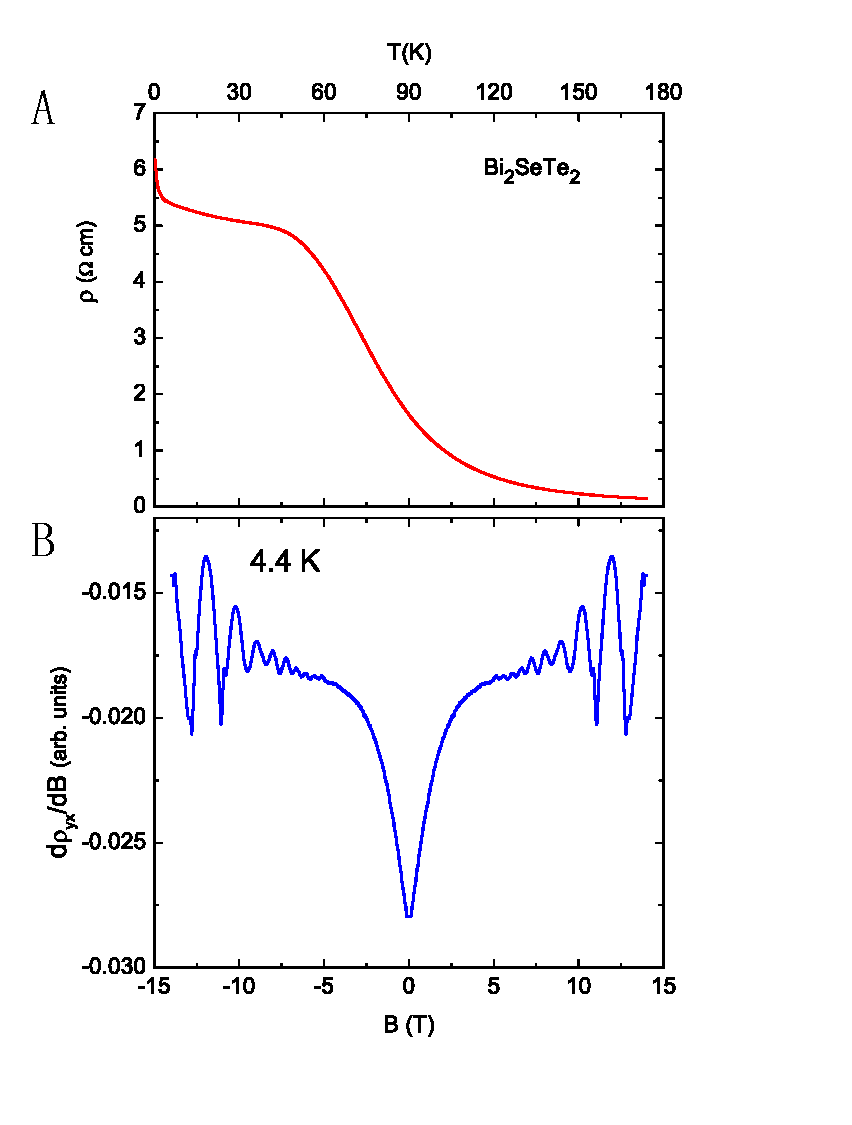
\includegraphics[width=0.9\linewidth]{ch-bts/figures/FigRvsT_lo.pdf} 
\caption{\label{figRvsT_lo}
The resistivity v.s. temperature curve and the derivative of the magnetoresistance curve of the bulk-insulating TI Bi$_2$Te$_2$Se.
Panel (A) shows $\rho$ vs. $T$ measured in $B$ = 0.  Below 10 K, $\rho$ 
reaches as high as 5.5 $\Omega$cm, or an areal
resistance $R_{\square}$ = 400 $\Omega$.  It was one of the most insulating TI crystals. The large resistivity indicates a very low bulk carrier density. Despite the non-metallic
value of $R_{\square}$, sizeable quantum oscillations are observed below 38 K.
Panel (B) displays the prominent SdH oscillations observed 
in the derivative $d\rho_{xy}/dB$ vs. $B$ at 4.4 K. Compared to Bi$_2$Te$_3$, the much larger SdH oscillations in Bi$_2$Te$_2$Se indicate a larger surface proportion of the current in the sample.
} 
  \end{center}
\end{figure}

A powerful way to study the properties of the energy band in a crystal is through the Shubnikovde Haas (SdH) oscillations in the magnetoresistance. High-quality SdH oscillations can uncover a lot of important information, such as the Fermi surface and the mobility of the bands. However, the sample needs to have a high mobility to generate SdH oscillations. In general, a sample with $\mu_b$ as low as 50 cm$^2$/Vs should not display Shubnikovde Haas oscillations in a magnetic field less than 14T. Surprisingly, however, the Hall resistivity $\rho_{yx}$ of our Bi$_2$Te$_2$Se sample displays prominent SdH oscillations that is resolved up to 38 K and down to 5 T. We have detected SdH oscillations in several crystals of Bi$_2$Te$_2$Se with $\rho$-$T$ profiles similar to that in Fig. \ref{figRvsT_lo}A. To emphasize the SdH oscillations, we display the the derivative $d\rho_{yx}/dT$ vs. $B$ at $T$ = 4.4 K in Fig. \ref{figRvsT_lo}B. It clear shows the high quality of the SdH oscillations. Independently, SdH oscillations were also observed in Bi$_2$Te$_2$Se by Y. Ando group~\cite{Ando10}. Since the bulk has a low mobility that could not generate SdH oscillations, we believe that the SdH oscillations originate from the surface states. We will discuss the analysis and reasons below. The work by Ren \etal~\cite{Ando10} also provides solid evidence the surface nature of the SdH oscillations by tracing the Fermi surface area in a tilted magnetic field.

Since the bulk still has a large carrier density, we believe that comparable surface conductance and bulk conductance coexist as parallel charge transport channels in Bi$_2$Te$_2$Se. To separate the bulk and surface contribution in the resistance measurement, it is convenient to convert resistance to conductance for the analysis. Since the total conductance $G$ is additive for parallel channels, the observed conductivity $\sigma_{ij}$ is
then the sum
\be
\sigma_{ij} = \sigma^b_{ij} + G^s_{ij}/d,
\label{eq:sigma}
\ee
where $\sigma^b_{ij}$ is the bulk conductivity and $G^s_{ij}$ is the conductance matrix of the surface states. The conductivity matrix $\sigma_{ij}$ is obtained by inverting the resistivity matrix $\rho_{ij}$. To isolate the SdH oscillations from the surface contribution in $\sigma_{xy}$, we define 
$\Delta\sigma_{xy} = \sigma_{xy} - \langle\sigma_{xy}\rangle$, where $\langle\sigma_{xy}\rangle$ is a smooth background. Here we use a low-power polynomial function to simulate and fit the background curve.


%%%%%%%%%%%%%%%%%%%%%%%%%%%%%%%%%%%%%%%%
%%%%%%%%%%%%%%%%%%%%%%%%%%%%%%%%%%%%%%%%
%%%%%%%%%%%%%%%%%%%%%%%%%%%%%%%%%%%%%%%%
%%%%%%%%%%%%%%%%%%%%%%%%%%%%%%%%%%%%%%%% FIGURE 

\begin{figure}[!htbp]
  \begin{center}            
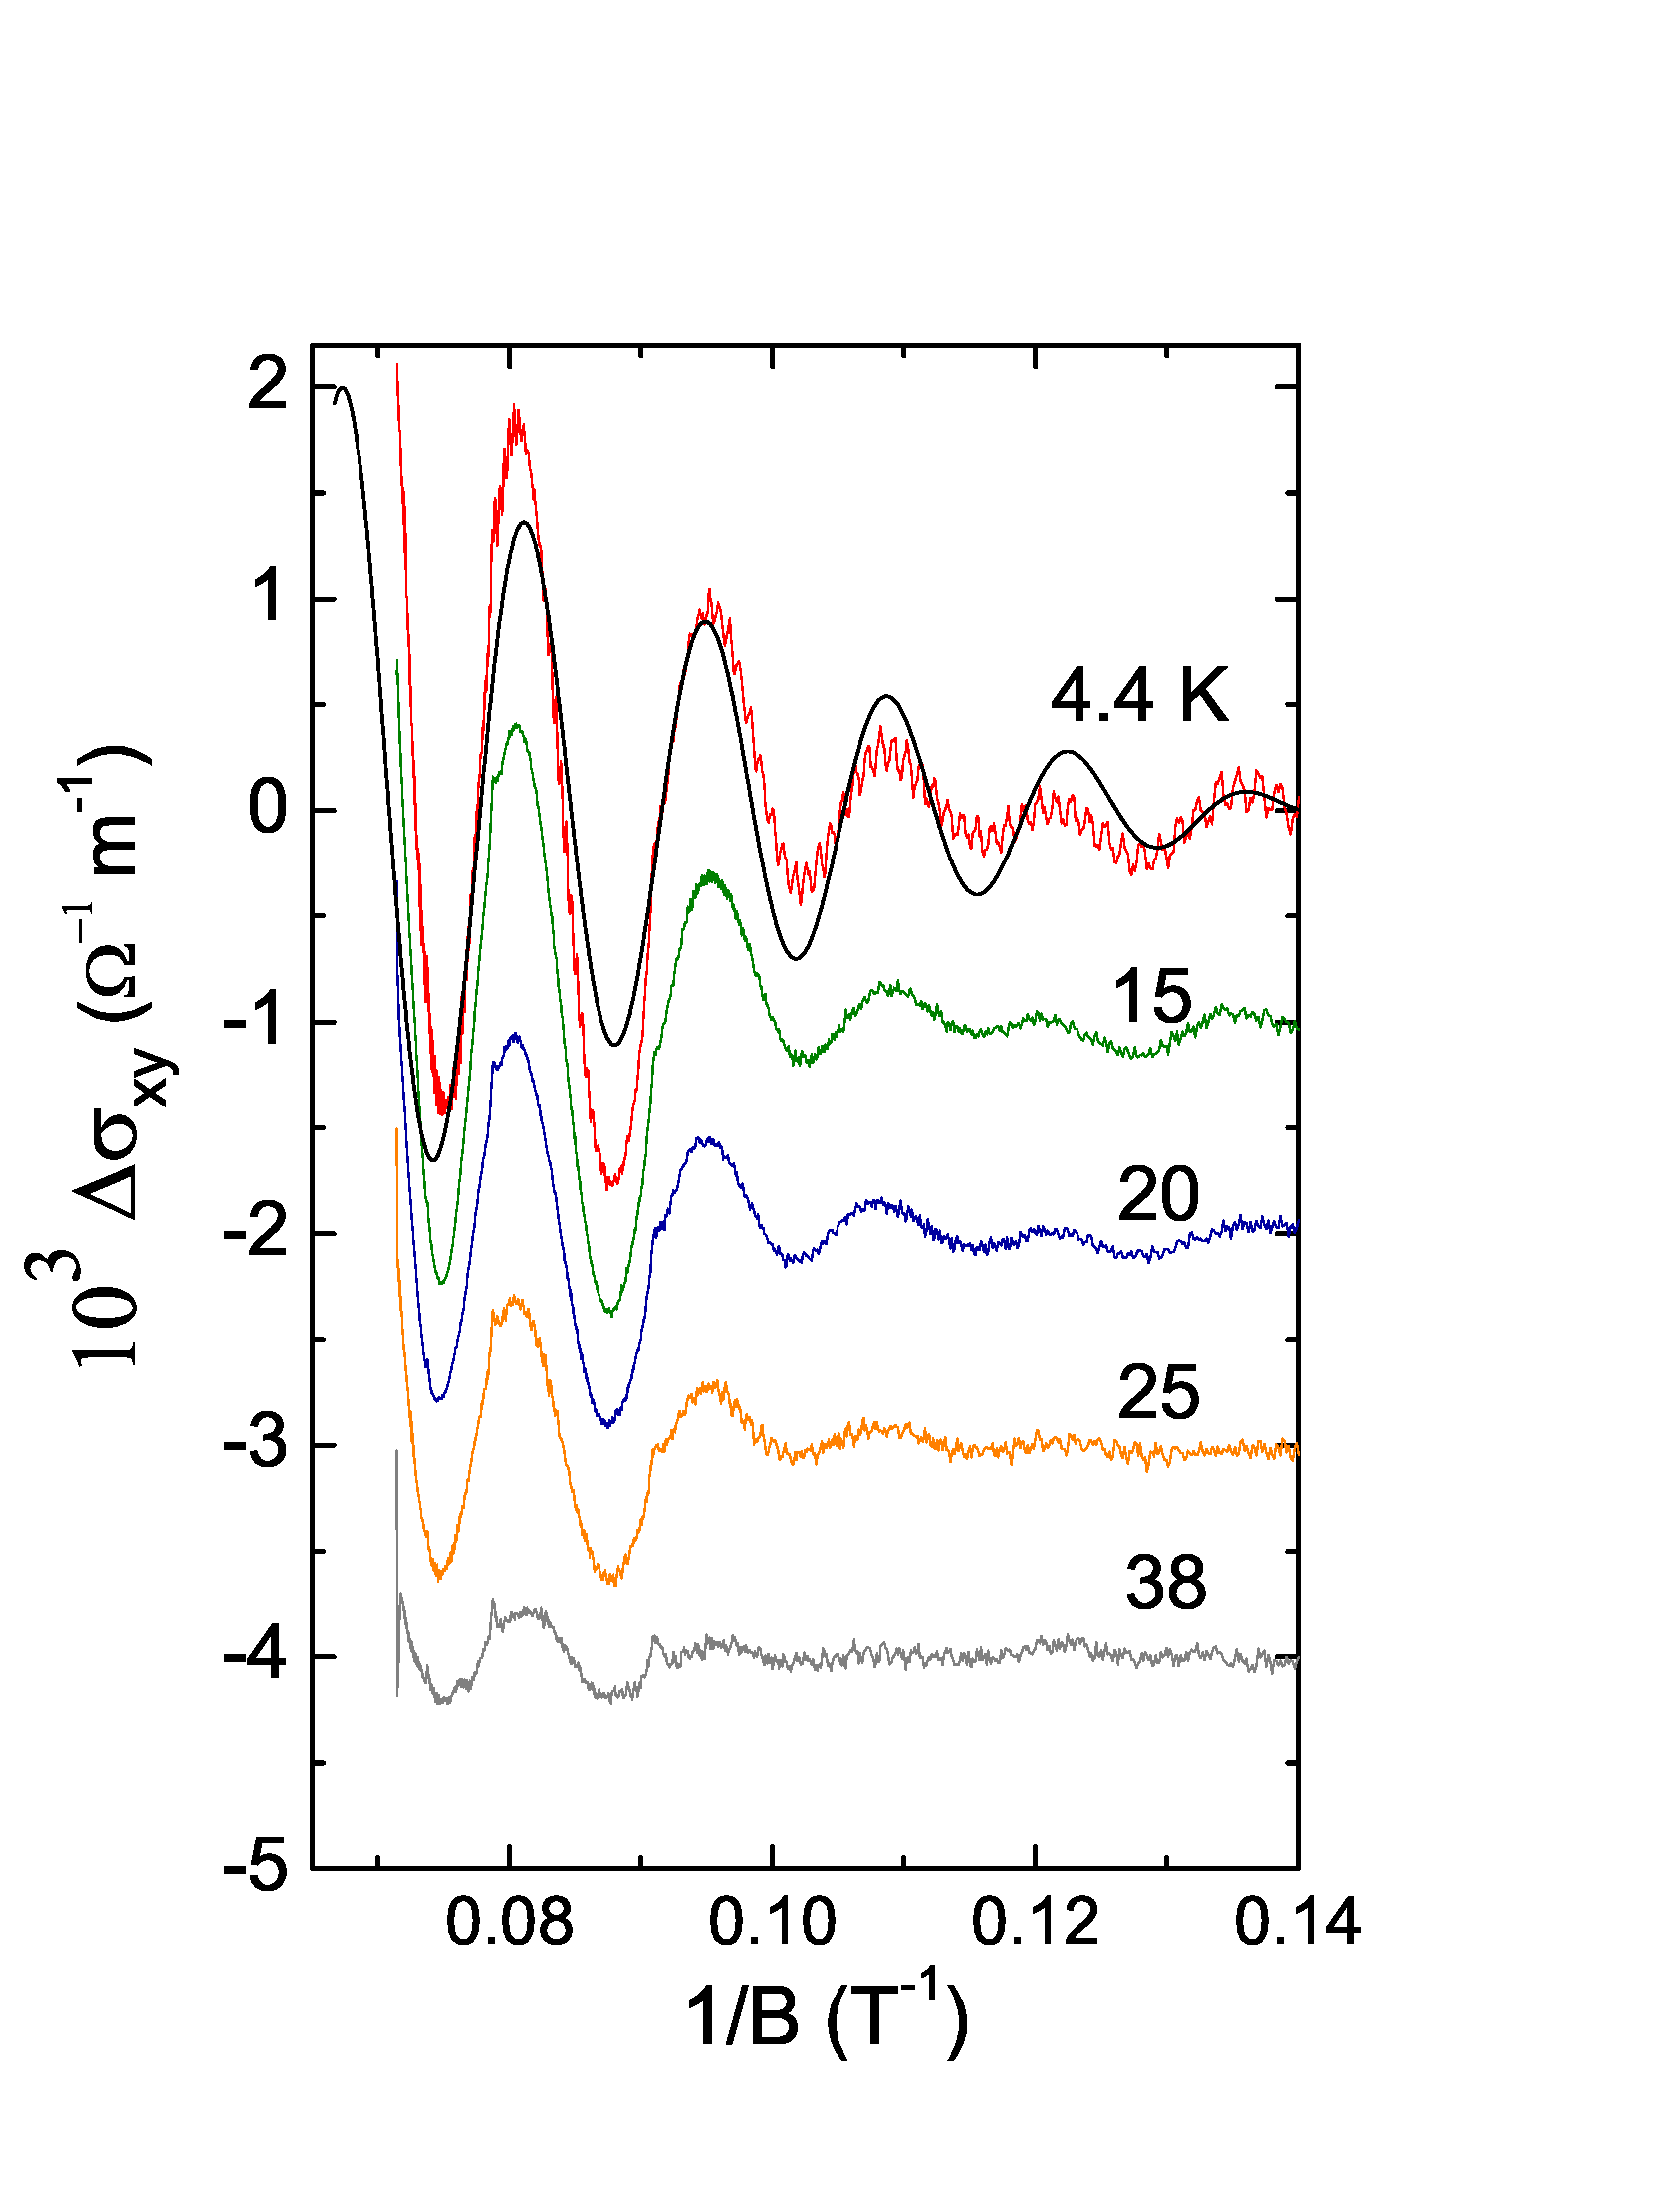
\includegraphics[width=0.9\linewidth]{ch-bts/figures/FigsxyT.eps}
\caption{\label{figsxy} 
Traces of the Hall conductivity $\Delta\sigma_{xy}$ 
(background subtracted) versus $1/B$ at selected $T$ for Bi$_2$Te$_2$Se.
The amplitudes of the oscillations decrease with an increasing $T$ but are still resolvable to 38 K.  
The smooth curve in the uppermost trace is a fit to $\Delta\sigma_{xy}$ by at 4.4 K 
using Eq. \ref{eq:sdh_hall}. The rapid decrease of the oscillation amplitudes for $1/B>$ 0.09 T$^{-1}$
reflects possible interference between 2 terms of similar amplitudes but slightly different
densities ($n_{s1},\;n_{s2}$) = (1.8, 1.7)$\times 10^{12}$ cm$^{-2}$.  
The fit yields the mobility $\mu$ = 2,800 cm$^2$/Vs and $k_F\ell$ = 41.This mobility is much higher than the one we obtained from the $\rho$ and the Hall density. Thus it indicates a different origin from the bulk states.
}
  \end{center}
\end{figure}


%%%%%%%%%%%%%%%%%%%%%%%%%%%%%%%%%%%%%%%%
%%%%%%%%%%%%%%%%%%%%%%%%%%%%%%%%%%%%%%%%
%%%%%%%%%%%%%%%%%%%%%%%%%%%%%%%%%%%%%%%%
%%%%%%%%%%%%%%%%%%%%%%%%%%%%%%%%%%%%%%%% FIGURE

\begin{figure}[!htbp]
  \begin{center}            
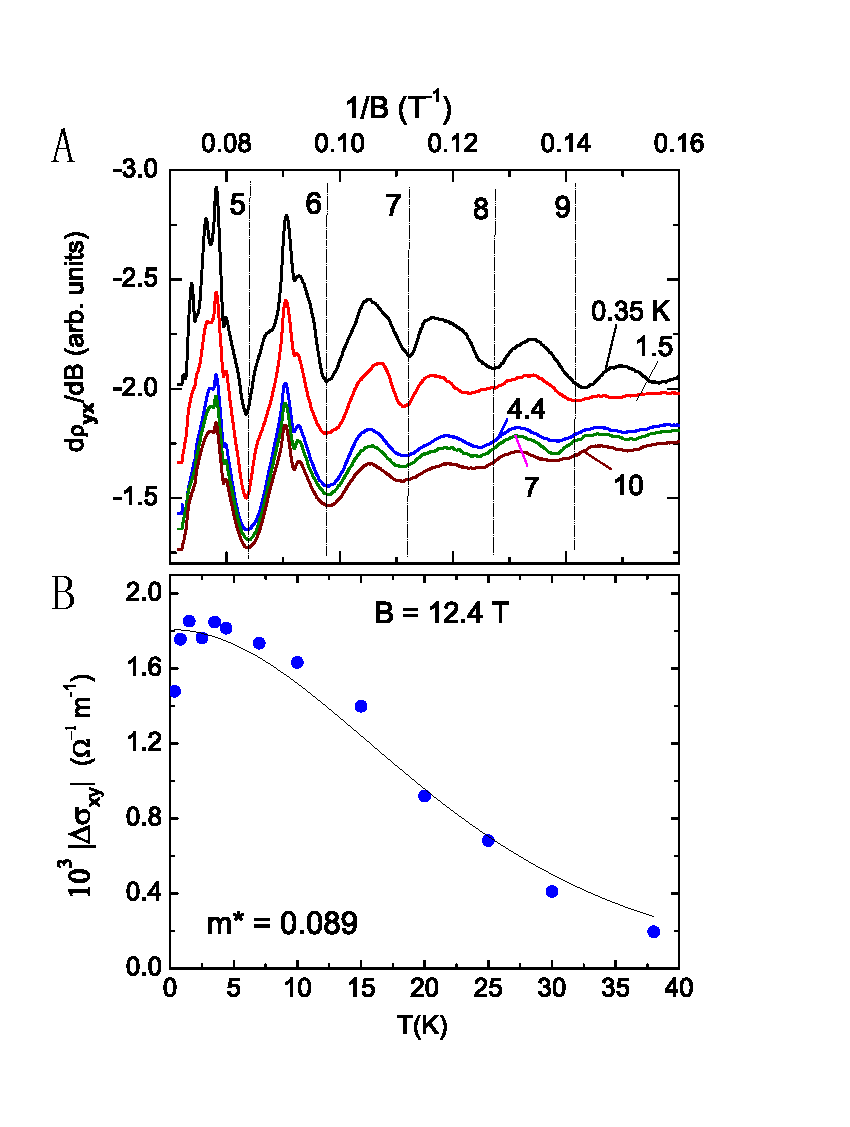
\includegraphics[width=0.9\linewidth]{ch-bts/figures/FigFitvsTemp.pdf} 
\caption{\label{figfit} (Color online) 
Panel (A) displays traces of the Hall resistivity 
$d\rho_{yx}/dB$ in Bi$_2$Te$_2$Se at 5 temperatures.  The minima in $|d\rho_{yx}/dB|$ are used to
fix the index field $B_{\nu}$ (dashed lines with $\nu$ indicated).  
For low LLs with $\nu<$6, there are extra peaks and deeps between the integer fillings, possibly related to some many-body states.
Panel (B) shows the fit of the peak positions versus $T$ with $B$ fixed at
12 T.  The fitting curve is based on Eq. \ref{eq:sdh_hall}. The fit yields $m^*$ = 0.089 $m_0$ (free mass).  With $k_F$ = 0.047 \AA$^{-1}$,
the inferred velocity $v_F$ = 6.0 $\times 10^5$ m/s.
} 
  \end{center}
\end{figure}

We show the background-subtracted conductivity $\Delta\sigma_{xy}$ versus $1/B$ at various temperatures (curves were measured at 13 temperatures in the range 0.3 $\le T\le$ 38 K) in Fig. \ref{figsxy}. On the $1/B$ axis, the oscillations have a clear period which indicates that they are SdH oscillations caused by the Landau level quantization. The SdH oscillations have large amplitudes below 10K, while the amplitudes decreases rapidly as $T$ increases above 10 K as expected by the Lifshitz-Kosevich theory for SdH oscillations.


We also fit the SdH oscillation curves to the standard Lifshitz-Kosevich expression~\cite{Jalan2010} 
\be
\frac{\Delta\sigma_{xy}}{\sigma_{xy}} = \left(\frac{\hbar\omega_c}{2E_F}\right)^{\frac12}
\frac{\lambda}{\sinh\lambda} e^{-\lambda_D}\cos
\left[\frac{2\pi E_F}{\hbar\omega_c}+\phi\right],
\label{eq:sdh_hall}
\ee
with $\lambda = 2\pi^2k_BT/\hbar\omega_c$ and $\lambda_D = 2\pi^2k_BT_D/\hbar\omega_c$,
where $\omega_c$ is the cyclotron frequency and 
the Dingle temperature is given by $T_D = \hbar/(2\pi k_B\tau)$,
with $\tau$ the lifetime.  Compared with
the SdH expression for the conductivity $\sigma_{xx}$, the phase $\phi$ in the 
Hall conductivity is shifted by $\pi/2$.
For the 2D electron gas, we may write the SdH frequency as
$2\pi E_FB/(\hbar\omega_c)$, which simplifies to $4\pi^2\hbar n_s/e$, with the 2D
carrier density $n_s = k_F^2/4\pi$ (per spin).  
As shown in Ref.~\cite{Gusynin2005}, Eq. \ref{eq:sdh_hall} may be employed in a Dirac system
if we write the cyclotron mass as $m_c = E/v_F^2$.  

As shown in Fig. \ref{figsxy}, we notice that it is not possible to get a reasonable fit for the SdH oscillations using one single SdH
frequency, as the SdH oscillation curves seem to have a beating pattern that come from two close frequencies.  For example, at $T<$ 6 K, the sharp decrease of the oscillation amplitudes for the range $B^{-1}>$ 0.12 T$^{-1}$ (the top curve in Fig. \ref{figsxy}) suggests a beating effect between two terms of nearly equal frequencies. Therefore we added another term to Eq. \ref{eq:sdh_hall} that is identical except for a slight difference in $n_s$ to fit the data. The measured curve of $\Delta\sigma_{xy}$ was fitted reasonably well with the 2 terms as shown by the first curve in Fig. \ref{figsxy} (the absolute value of the surface Hall conductance $G_{xy}$ is not known). In our fitting, there are 5 adjustable parameters ($n_{si}$ and amplitude $A_i$, with $i$ = 1,2) and $T_D$ (assumed same for both). The best fit (top curve in Fig. \ref{figsxy}) is obtained with $A_1 = A_2$ and and densities differing by only 5$\%$ [$(n_{s1}, n_{s2})$ = (1.79, 1.71)$\times 10^{12}$ cm$^{-2}$], corresponding to an average Fermi wavevector $k_F$ = 0.047 \AA$^{-1}$. The fit yields $T_D$ = 8.5$\pm$1.5 K, which corresponds to a mean-free-path $\ell$ = 70-100 nm and a surface mobility $\mu_s = e\ell/\hbar k_F$ = 2,800$\pm$250 cm$^2$/Vs. It indicates that the surface mobility $\mu_s$ significantly exceeds the bulk $\mu_b$ by a factor of $\sim$60. By fitting to the decrease of amplitudes with $T$ at a fixed $B$ (12.4 T), we also get the effective mass $m^*$ = 0.089 $m_e$ (Fig. \ref{figfit}B).  Combined with $k_F$, we obtain a Fermi velocity $v_F\sim$ 6 $\times 10^5$ m/s, higher than that in Bi$_2$Te$_3$. This $v_F$ value is consistent with the one for the surface states observed in the ARPES experiment ~\cite{BTS_ARPES}.


We argue that the high mobility here gives strong evidence for the surface nature of the SdH oscillations in Bi$_2$Te$_2$Se. Otherwise if the oscillations were from the bulk states, the SdH period would then yield a 3D Fermi sphere of radius $k_F$ = 0.047 \AA$^{-1}$, or a 3D density of 3.3$\times 10^{18}$ cm$^{-3}$.  The inferred $\mu$ then would imply a 3D resistivity $\rho_b \sim$ 0.7 m$\Omega$cm at 4.4 K. The large discrepancy (factor of 9,000) from the observed value strongly disagree with a bulk origin for the SdH oscillations. Besides, Ref. ~\cite{Ando10} has measured the SdH oscillations of Bi$_2$Te$_2$Se in a tilted magnetic field. The angle dependence of the measured periods show that the implied Fermi surface (FS) is consistent with the behavior of a 2D FS instead of a 3D one.

These evidences make us believe that the SdH oscillations in our Bi$_2$Te$_2$Se samples come from the high-mobility surface carriers. Also since the SdH oscillations of a 2D electron gas only appear when $\bf B$ is perpendicular to the 2D plane, the two periods are likely from the large top and bottom surfaces of the cleaved crystal that are normal to $\bf B$.  Inferred from $n_{s1}$ and $\mu$, we find
that the conductance of each surface is $G_s = \frac12(e^2/h)k_F\ell \simeq$ 0.72 mS (or $R_{\square}\sim$ 1.39 k$\Omega$). As a result, we infer that the surface conductance accounts for $\sim 60\%$ of the observed conductance at 4 K. 




%%%%%%%%%%%%%%%%%%%%%%%%%%%%%%%%%%%%%%%%
%%%%%%%%%%%%%%%%%%%%%%%%%%%%%%%%%%%%%%%%
%%%%%%%%%%%%%%%%%%%%%%%%%%%%%%%%%%%%%%%%
%%%%%%%%%%%%%%%%%%%%%%%%%%%%%%%%%%%%%%%% FIGURE

\begin{figure}[!htbp]
  \begin{center}            
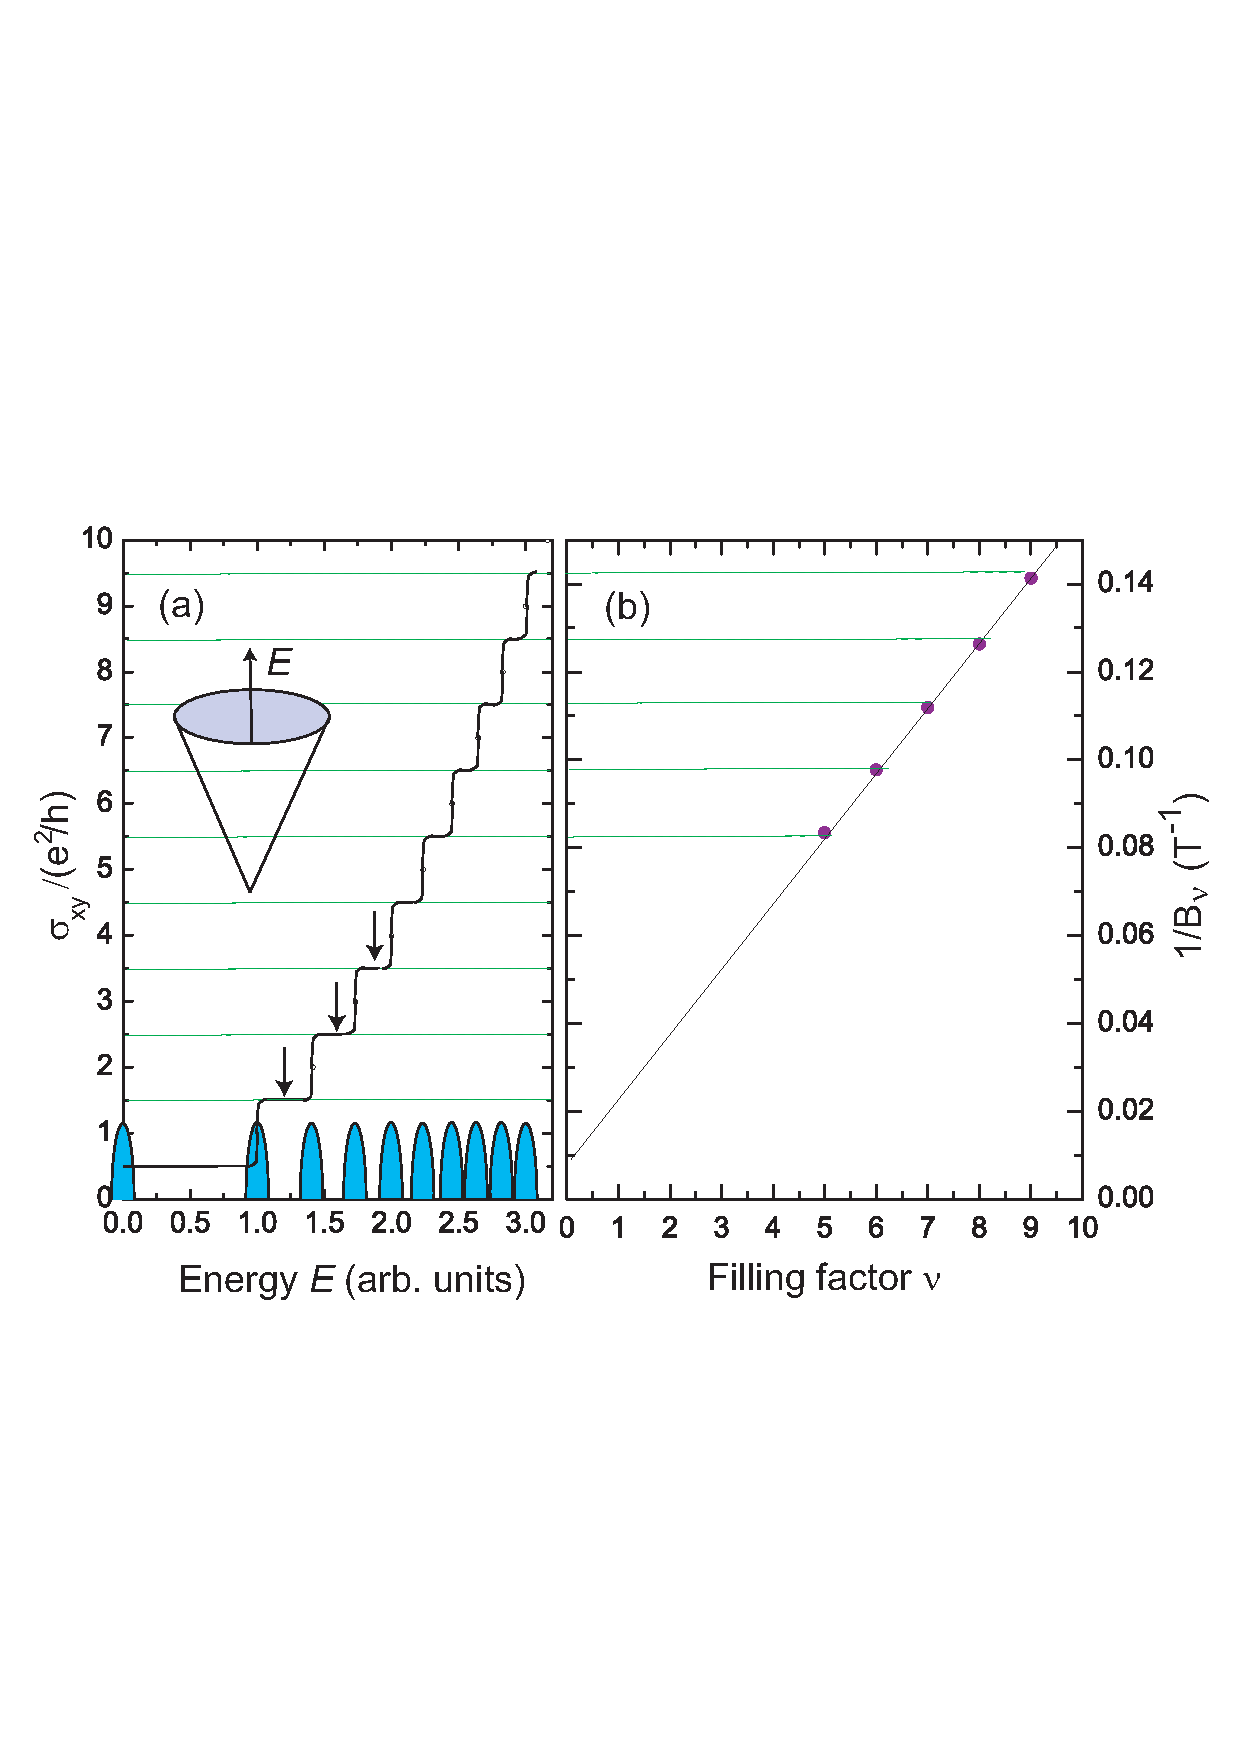
\includegraphics[width=0.9\linewidth]{ch-bts/figures/FigDiracIndex2.pdf} 
\caption{\label{figindex} 
Construction used to fix the filling factors for a Dirac spectrum.  Panel (a) depicts how the Landau indices are decided for a 2D Dirac gas in the quantum Hall regime. It sketches
schematically the step-like increase of $\sigma_{xy} = (e^2/h)[\nu+\frac12]$ versus energy $E$,
where $\frac12$ arises from the $\nu$ = 0 LL at the Dirac point.
The half-ovals are broadened Landau Levels centered at $E_{\nu}=\hbar\ell_B^{-1} v_F\sqrt{2\nu}$.
$B_{\nu}$ are the fields at which $E_F$ falls between LLs (arrows).  The inset
shows the 2D Dirac energy surface in zero $B$.  In Panel (b), we compare this definition of filling factors $\nu$ with
the measured values of $1/B_{\nu}$.
The 5 values of $1/B_{\nu}$ fall on a straight line 
that intercepts the $\nu$ axis at -0.55. The intercept that is close to $\frac{1}{2}$ (mod 1) is consistent with a Dirac spectrum.  
} 
  \end{center}
\end{figure}

Compared to those in Bi$_2$Te$_3$, the SdH oscillations in Bi$_2$Te$_2$Se are much more outstanding. Such prominent oscillations also provide us an opportunity to address whether the surface states' dispersion is Dirac like or not. The previous results on Bi$_2$Te$_3$ have some ambiguity on this issue due to the small amplitudes of the oscillations. In principle, one may plot the
"index" field $1/B_{\nu}$ versus the filling factors $\nu = 1,2 \cdots$, and track the intercept in the limit $B\to\infty$.  Nevertheless, one needs to be careful about whether to take the maxima or minima of $\rho_{xx}$ or $\rho_{yx}$ for the index fields when the sample is not in the quantum Hall regime. Also, as we will discuss in the next subsection, the mixing with a large bulk conductivity will also make this problem even more subtle.  Here we define the index field $B_{\nu}$ as the field at which the chemical potential $E_F$ falls between 2 LLs. The definition could be changed but it should be consistent in $\sigma_{ij}$ and $\rho_{ij}$, and it should agree with the quantum Hall limit as well. With our definition, when the applied field is $B=B_{\nu}$ in the quantum Hall limit, the Hall conductivity has plateau values $\sigma_{xy} = (e^2/h)(\nu+\frac12)$ for the Dirac electrons (compared with $\sigma_{xy} = \nu e^2/h$ for the Schr\"{o}dinger ones). As a result, the index plot n \emph{v.s.} $1/B_{\nu}$ of the Dirac electrons has an intercept of $\frac{1}{2}$ (mod 1) on the $n$-axis, while that of Schr\"{o}dinger electrons intercept 0. In Bi$_2$Te$_2$Se, the large amplitudes could help us determine the "index" field more accurately and thus reduce the uncertainties in the extrapolated intercept.




%%%%%%%%%%%%%%%%%%%%%%%%%%%%%%%%%%%%%%%%
%%%%%%%%%%%%%%%%%%%%%%%%%%%%%%%%%%%%%%%%
%%%%%%%%%%%%%%%%%%%%%%%%%%%%%%%%%%%%%%%%
%%%%%%%%%%%%%%%%%%%%%%%%%%%%%%%%%%%%%%%% FIGURE

\begin{figure}[!htbp]
  \begin{center}            
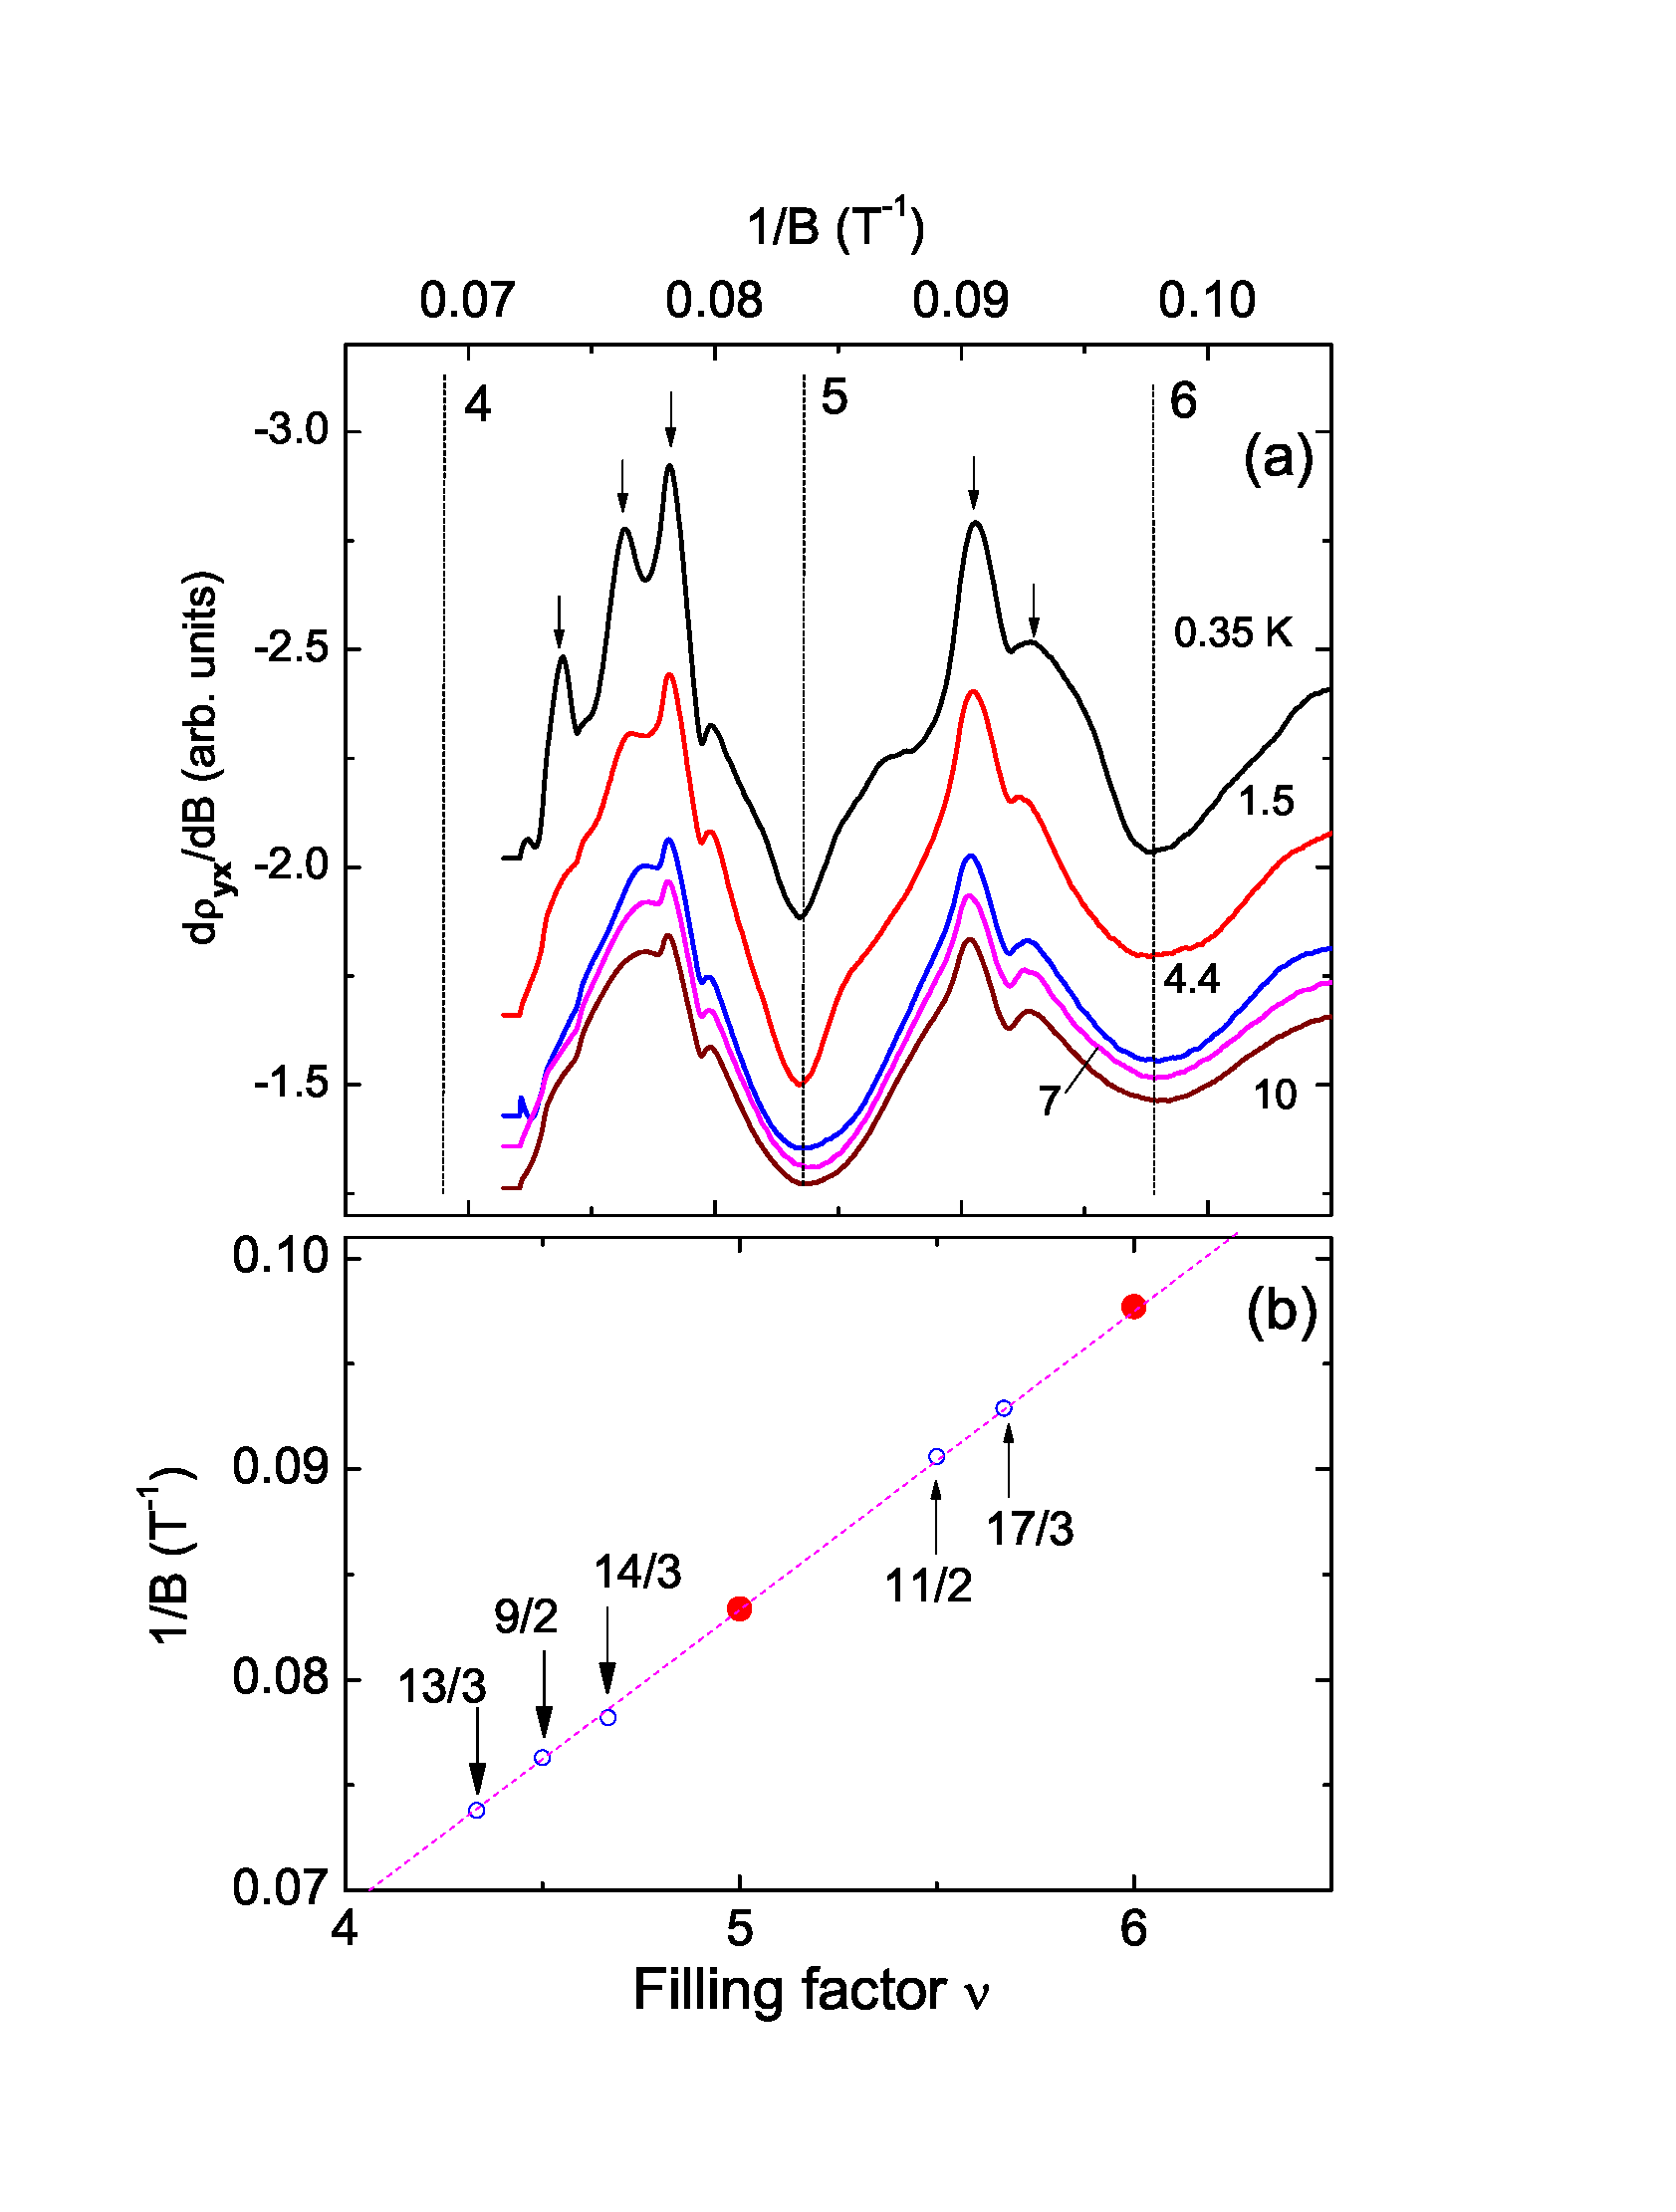
\includegraphics[width=0.9\linewidth]{ch-bts/figures/FigrhoxyExpand.eps} 
\caption{\label{figexpand} 
The possible fractional filling states in the SdH oscillations.
Panel (a): Expanded view of $d\rho_{yx}/dB$ of Bi$_2$Te$_2$Se for 4$<\nu<$6 shows sharp
maxima at non-integer values of $\nu$, at $T$ from 0.35--10 K. The feature decreases rapidly with an increasing temperature. The arrows
locate the more prominent peaks.  In Panel (b), the peak positions plotted
against $\nu$ align well with fractional values of $\nu$ (arrows mark the values
$\nu$ = 13/3, 9/2, $\cdots$, 17/3). 
}
  \end{center}
\end{figure}


Fig. \ref{figindex} is a sketch that relates the index plot ($1/B_{\nu}$ vs. $\nu$) and the Hall plateaus to the Dirac energy spectrum.  
Fig. \ref{figindex}a shows the steps of the quantized Hall conductivity $\sigma_{xy}/(e^2/h)$ versus the Fermi energy $E_F$,  where the shift of $\frac12$ arises from the $\nu = 0$ LL at the Dirac point, as in graphene. The half-ovals drawn on the $E$-axis represent the broadened LLs.  As the density of states (DOS) reaches the peaks at the step-edges of $\sigma_{xy}$, $d\rho_{yx}/dB$ also reaches the maxima. Consequently, the minima in $|d\rho_{yx}/dB|$ locate $B_{\nu}$, the field at which $E_F$ lies between LLs (arrows) as we defined. The $\frac12$-shift of the intercept implies that the line of $1/B_{\nu}$ vs. $\nu$ in Panel (b) does not pass through the origin (whereas it does for a quadratic dispersion).


To find the intercept for our Bi$_2$Te$_2$Se sample, we plot the measured $1/B_{\nu}$ versus $\nu$ in Fig. \ref{figindex}b.
With just one vertical scale adjustment, we can align the 5 data points to the steps in Panel (a).  At our highest $B$, the filling factor is $\nu$ = 5.
The straight line fitted to the data in (b) noticeably intercepts the $\nu$ axis at $\nu$ = -0.55 instead of 0, consistent with the $\frac12$ shift expected from a Dirac spectrum.  

Another possibly interesting point in our data is the additional peaks in the oscillations. Recently, Analytis \etal~\cite{Analytis} reported possibly fractional-filling states in (Bi,Sb)Se$_3$ in very intense fields ($B>$50 T). We also find some similar evidence for fractional-filling states that
emerge at much lower fields (11 T).  Fig. \ref{figexpand}a shows an intriguing array of sharp \emph{maxima} in $d\rho_{yx}/dB$ (arrows) that is apparent for 4$<\nu <$6. The peaks become weaker as $T$ increases from 0.35 K, but some 
are still resolved even at 10 K.  Interestingly, we notice that the peak positions align well with fractional values of $\nu$, as shown in Fig. \ref{figexpand}b. But these fractional features may need more detailed study in samples with higher mobilities. Unfortunately, as we will see in the next subsection, these features do not appear in our samples in a higher magnetic field. Further investigation may needed with samples of higher quality.

\section{Approaching the Lowest Landau Level and Evidence for $\pi$ Berry Phase in 45T}
\label{sec:bts:result14T}
\subsection{Prepare for the High Field Experiments}\label{hifield_intro}
%Everyone needs floating figures in their dissertation. 
%
%As shown in Figure~\ref{fig:pastwork:titlepage}, the Mudd Library dissertation requirements~\cite{muddthesis2009} specify additional options for formatting the title page. For example, if your thesis has multiple volumes, or to indicate the proper formatting for a master's thesis.
%
%\begin{figure}[htb]
%  \begin{center}
%    
\includegraphics[width=0.9\linewidth]{ch-bts/figures/titlepage}
%    \caption[Sample Title Page Layout]{Sample title page layout~\cite{muddthesis2009}}
%    \label{fig:pastwork:titlepage}
%  \end{center}
%\end{figure}
The 14T data have demonstrated that the surface states on Bi$_2$Te$_2$Se could be well resolved by quantum oscillations due to the large $G^s / G^b$ ratio. However, at 14T, the lowest Landau index of the Bi$_2$Te$_2$Se's surface states is still far away from 0. As a result, the extrapolated intercept of the Landau indices when $1/B\to 0$  is not well resolved. Since the intercept is important for obtaining the Berry phase of the Dirac surface states, it's of great value to approach the lowest Landau level at a higher magnetic field. Besides, the transport experiments close to and at the quantum limit are important for the search of novel interacting physics of the Dirac surface states.

When a strong magnetic field $\bf B$ is applied normal to the surface,
the Dirac states form quantized Landau Levels (LLs) and generate oscillations in the surface conductance $G^s$. To clear any confusion on the symbols, we define the "index field" $B_n$ as the field at which the chemical potential $\mu$ lies between two LLs. This means that the surface states are in the "energy gap" sandwiched by two Landau levels at the field $B_n$. Thus $G^s$ reaches minima at such $B_n$ while the corresponding total resistance $R_{xx}$ reaches maxima if the Hall angle is small as the case here. 
%A plot of the integers $n$ vs. $1/B_n$ gives a nominally straight line with slope equal to
%the FS cross-section $S_F$.  


As we discussed in previous sections, the Landau index plot of $n$ \emph{v.s.} $1/B_n$ will be linear in both Schr\"{o}dinger's case and Dirac's cases. The slope of the fitting line could also give us the Fermi surface cross section $S_F$. The difference between the two cases happens in the limit
$1/B_n\to 0$. In the Schr\"{o}dinger case, there are $n$ filled LLs below $E_F$ when the field equals $B_n$ (as defined).
In comparison, the Dirac electrons have 
$n+\frac12$ filled LLs between $E_F$ and the Dirac point (at $E$ = 0). The extra $\frac12$ Landau level lies right at the Dirac point. It is fixed at the Dirac point because it has equal contributions from both the conduction and valence band, as each contributes half of the states in the $n$ = 0 LL. Therefore, the Landau index line $1/B_n$ vs. $n$ has different intercepts for the Dirac and Schr\"{o}dinger cases. The Dirac electron has an intercept $\gamma = -\frac12$ while the Schr\"{o}dinger electron's $\gamma$ is 0. The additional $\frac12$-shift of Dirac electrons has been confirmed in the quantum Hall effect of graphene~\cite{Kim}. A difference between graphene and the topological insulator is that graphene has four folds of Dirac electrons, while TI only has one for each of the two surfaces.





%%%%%%%%%%%%%%%%%%%%%%%%%%%%%%%%%%
%%%%%%%%%%%%%%%%%%%%%%%%%%%%%%%%%%
%%%%%%%%%%%%%%%%%%%%%%%%%%%%%%%%%% FIGURE 1
\begin{figure}[!htbp]
  \begin{center}
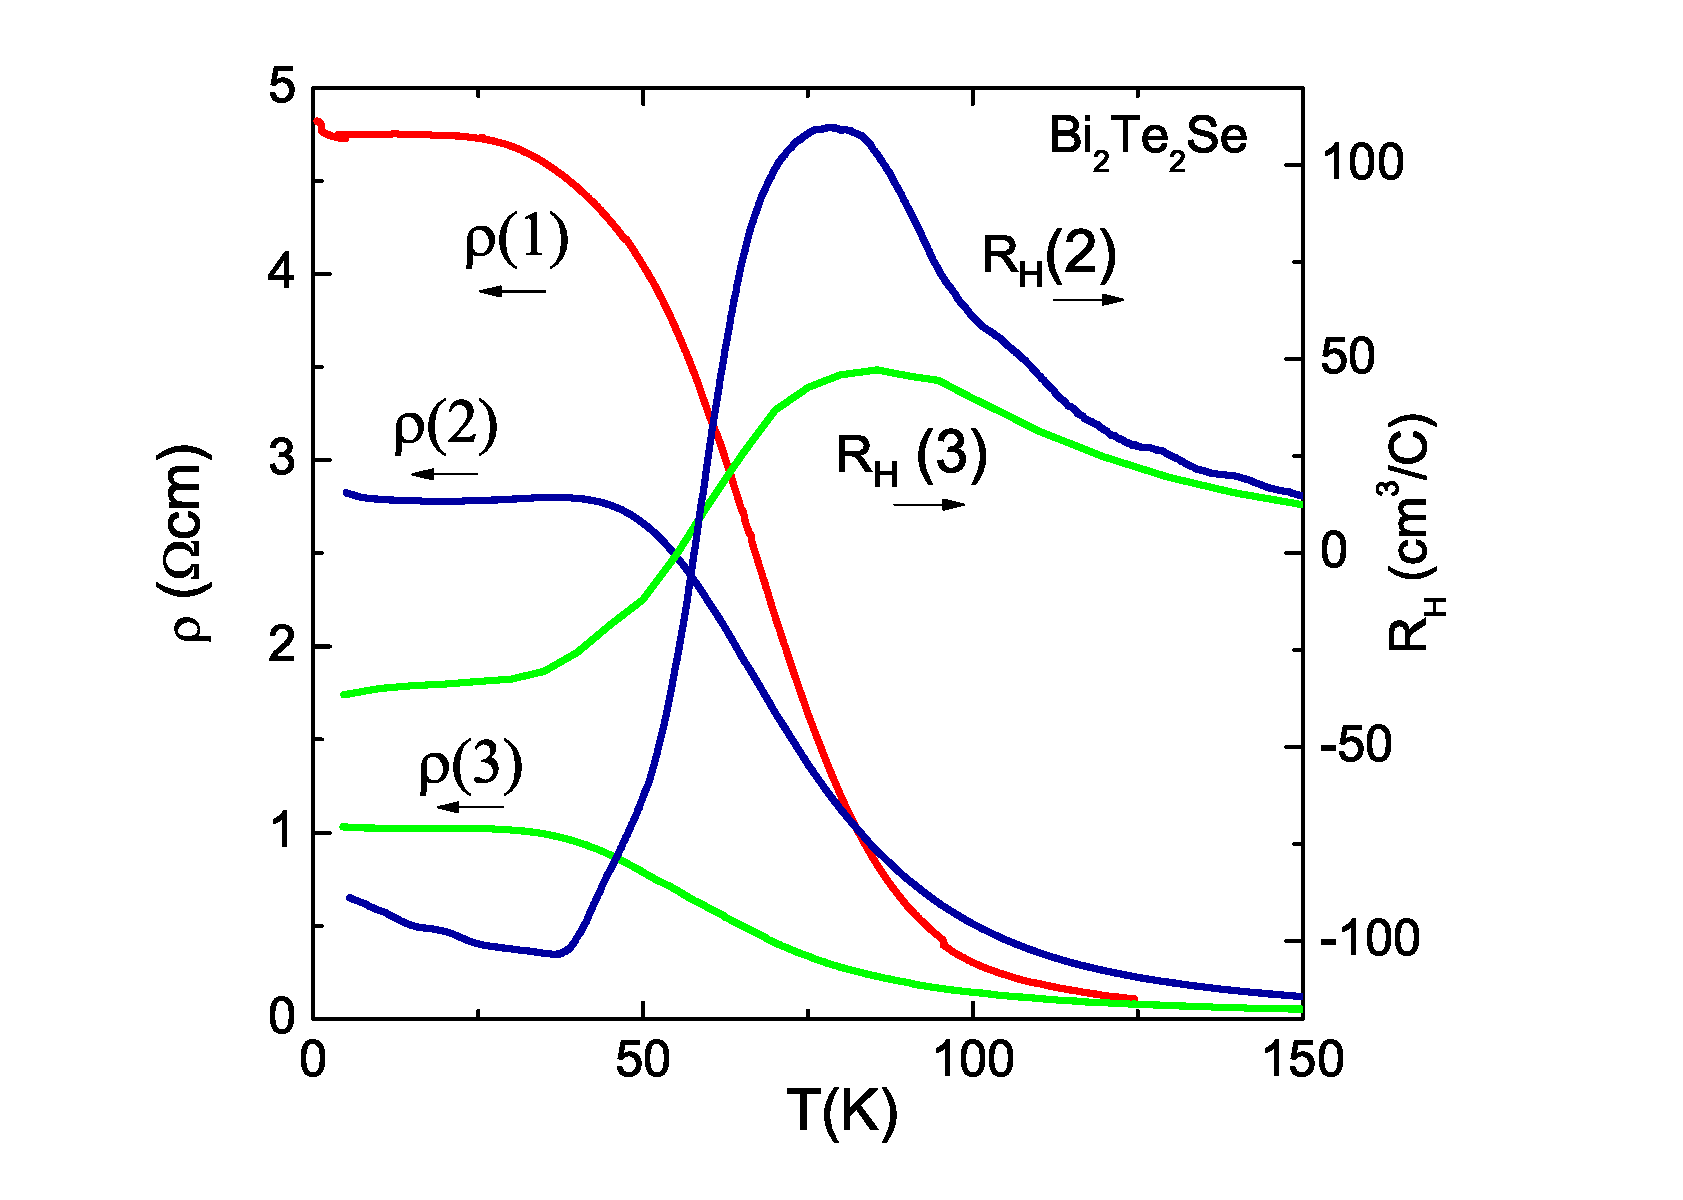
\includegraphics[width=0.9\linewidth]{ch-bts/figures/FigRvsT.eps}
\caption{\label{figRvsT} (color online)
The observed resistivity $\rho$ and Hall coefficient $R_H$ vs. $T$ in Bi$_2$Te$_2$Se for Sample 1, 2, 3. The magnitudes of
$\rho$ and $R_H$ at 4 K vary considerably between annealed samples. But all the samples have an insulating $R-T$ dependence with some $n$-type carriers at 4K. The change in sign of $R_H$ 
near 56 K reflects the thermal activation of bulk hole carriers across a gap of 50 mV.
The largest SdH amplitudes are observed in samples with $\rho >$ 4 $\Omega$cm at 4 K.
}
  \end{center}
\end{figure}
%%%%%%%%%%%%%%%%%%%%%%%%%%%%%%%%%%

Another issue we hope to address here is the Zeeman energy and g-factor of the surface states on Bi$_2$Te$_2$Se. While the strict particle-hole symmetry implies that the lowest Landau level is unshifted in energy, a large Zeeman energy $g\mu_BB$, where $g$ is the surface Lande g-factor and $\mu_B$ is the Bohr magneton, may lead to a high-field distortion of the SdH period and thus a distortion on the Landau index plot. There are some debates on the strength of the Zeeman energy in previous experiments. For example, the in-field STM experiments ~\cite{Hanaguri,Xue10} have shown that the $n$ = 0 LL is unshifted in energy up to 11 Tesla, while Ref~\cite{Taskin} inferred a $g$ factor as large as 76 from the low-field SdH oscillations in transport experiments. Some other quantum oscillation experiments~\cite{Qu,Analytis} had limited resolution due to the bulk contribution. Here we could explore this issue in SdH experiments at a much larger $B$ and with a lower Landau index. The low bulk carrier density in Bi$_2$Te$_2$Se also increases our resolution.

\subsection{Resistivity maxima or minima?}\label{maxmin}
As we mentioned above, the index field $B_n$ plays the key role in determining the intercept shift and the Berry phase in the Landau index plot. While the case for an ideal two-dimensional electron gas(2DEG) is clear in quantum Hall effect, it is important to discuss this issue when the surface and bulk carriers coexist and both contribute a large portion of the total conductance. In the current Bi-based 3D topological insulators, the bulk electrons or holes provide a current channel parallel to that of the surface states. By contrast, the current carried by the 2DEG in graphene and GaAs heterostructures is not mixed with any bulk channels. Thus when $E_F$ falls between two adjacent LLs in the QHE regime of graphene, both the 2D longitudinal conductance $G_{xx}$ and resistance $R_{xx}$ attain a deep minimum (this follows from $R_{yx}\gg R_{xx}$) while $G_{xy}$ and $R_{yx}$ reach finite quantized values. 


%The index field $B_n$ clearly plays the key role in pinning down the -$\frac12$ shift in the index plot. 
%Here we wish to discuss the question of determining $B_n$ when surface and bulk carriers co-exist~\cite{Fu}. 
%In the bismuth-based systems (and other 3D topological insulators), 
%the two-dimensional electron gas (2DEG) on the surface is in intimate contact 
%with bulk electrons which conduct a significant fraction of the 
%applied current. By contrast, the entire current is carried by the 2DEG in graphene 
%and GaAs heterostructures. When $E_F$ falls between adjacent LLs in the QHE regime of graphene, 
%both the 2D conductance $G_s$ and resistance $R_{xx}$ attain 
%a deep minimum (this follows from $R_{yx}\gg R_{xx}$). 


However, the situation becomes subtle when a large
bulk conduction channel exists in parallel (as the case here). The observed conductance matrix
becomes the sum of both the bulk and the surface part, i.e.
\be
G_{ij} = G^s_{ij} + G^b_{ij},
\label{eq:G}
\ee
where $G^b_{ij}$ is the bulk conductance matrix. In Bi$_2$Te$_2$Se, the bulk carriers have a very low mobility ($\mu_b$ ~ 50 cm$^2$/Vs), therefore they do not contribute to the quantum oscillations even at 45T. The additivity of the conductances in Eq. \ref{eq:G} implies that the index fields $B_n$ we defined still correspond to minima in $G_{xx}$. However, due to the large amount of bulk carriers, the bulk $G^b_{xx}$ is dominant. Since $G^b_{xx}$ has a gentle field dependence, the observed resistance now reaches maxima at $B_n$, since $R_{xx} = G_{xx}/[G_{xx}^2+G_{xy}^2]\sim 1/G_{xx} = 1/(G^b_{xx}+G^s_{xx})$. Hence it is less confusing to use the conductance tensor $G_{ij}$ to find the index field $B_n$ because the bulk and surface contribution are additive. We will use this paradigm to analyze our experimental results below. 

When the Hall resistance is not available, as in many experiments, one may still use the SdH oscillations in the longitudinal resistance $R_{xx}$ along, provided $B_n$ is identified with its \emph{maxima}. It is equivalent to converting $R_{xx}$ into $G_{xx} \sim 1/R_{xx}$ if the Hall signal is small compared to $R_{xx}$. It is important to take such care in determining the real index intercept of TI's quantum oscillations, because if people otherwise mistakenly identify $B_n$ with \emph{minima} in $R_{xx}$, a spurious -$\frac12$ intercept will appear for carriers with a Schr\"{o}dinger dispersion.




%%%%%%%%%%%%%%%%%%%%%%%%%%%%%%%%%%
%%%%%%%%%%%%%%%%%%%%%%%%%%%%%%%%%%
%%%%%%%%%%%%%%%%%%%%%%%%%%%%%%%%%% FIGURE 2
\begin{figure}[!htbp]
  \begin{center}
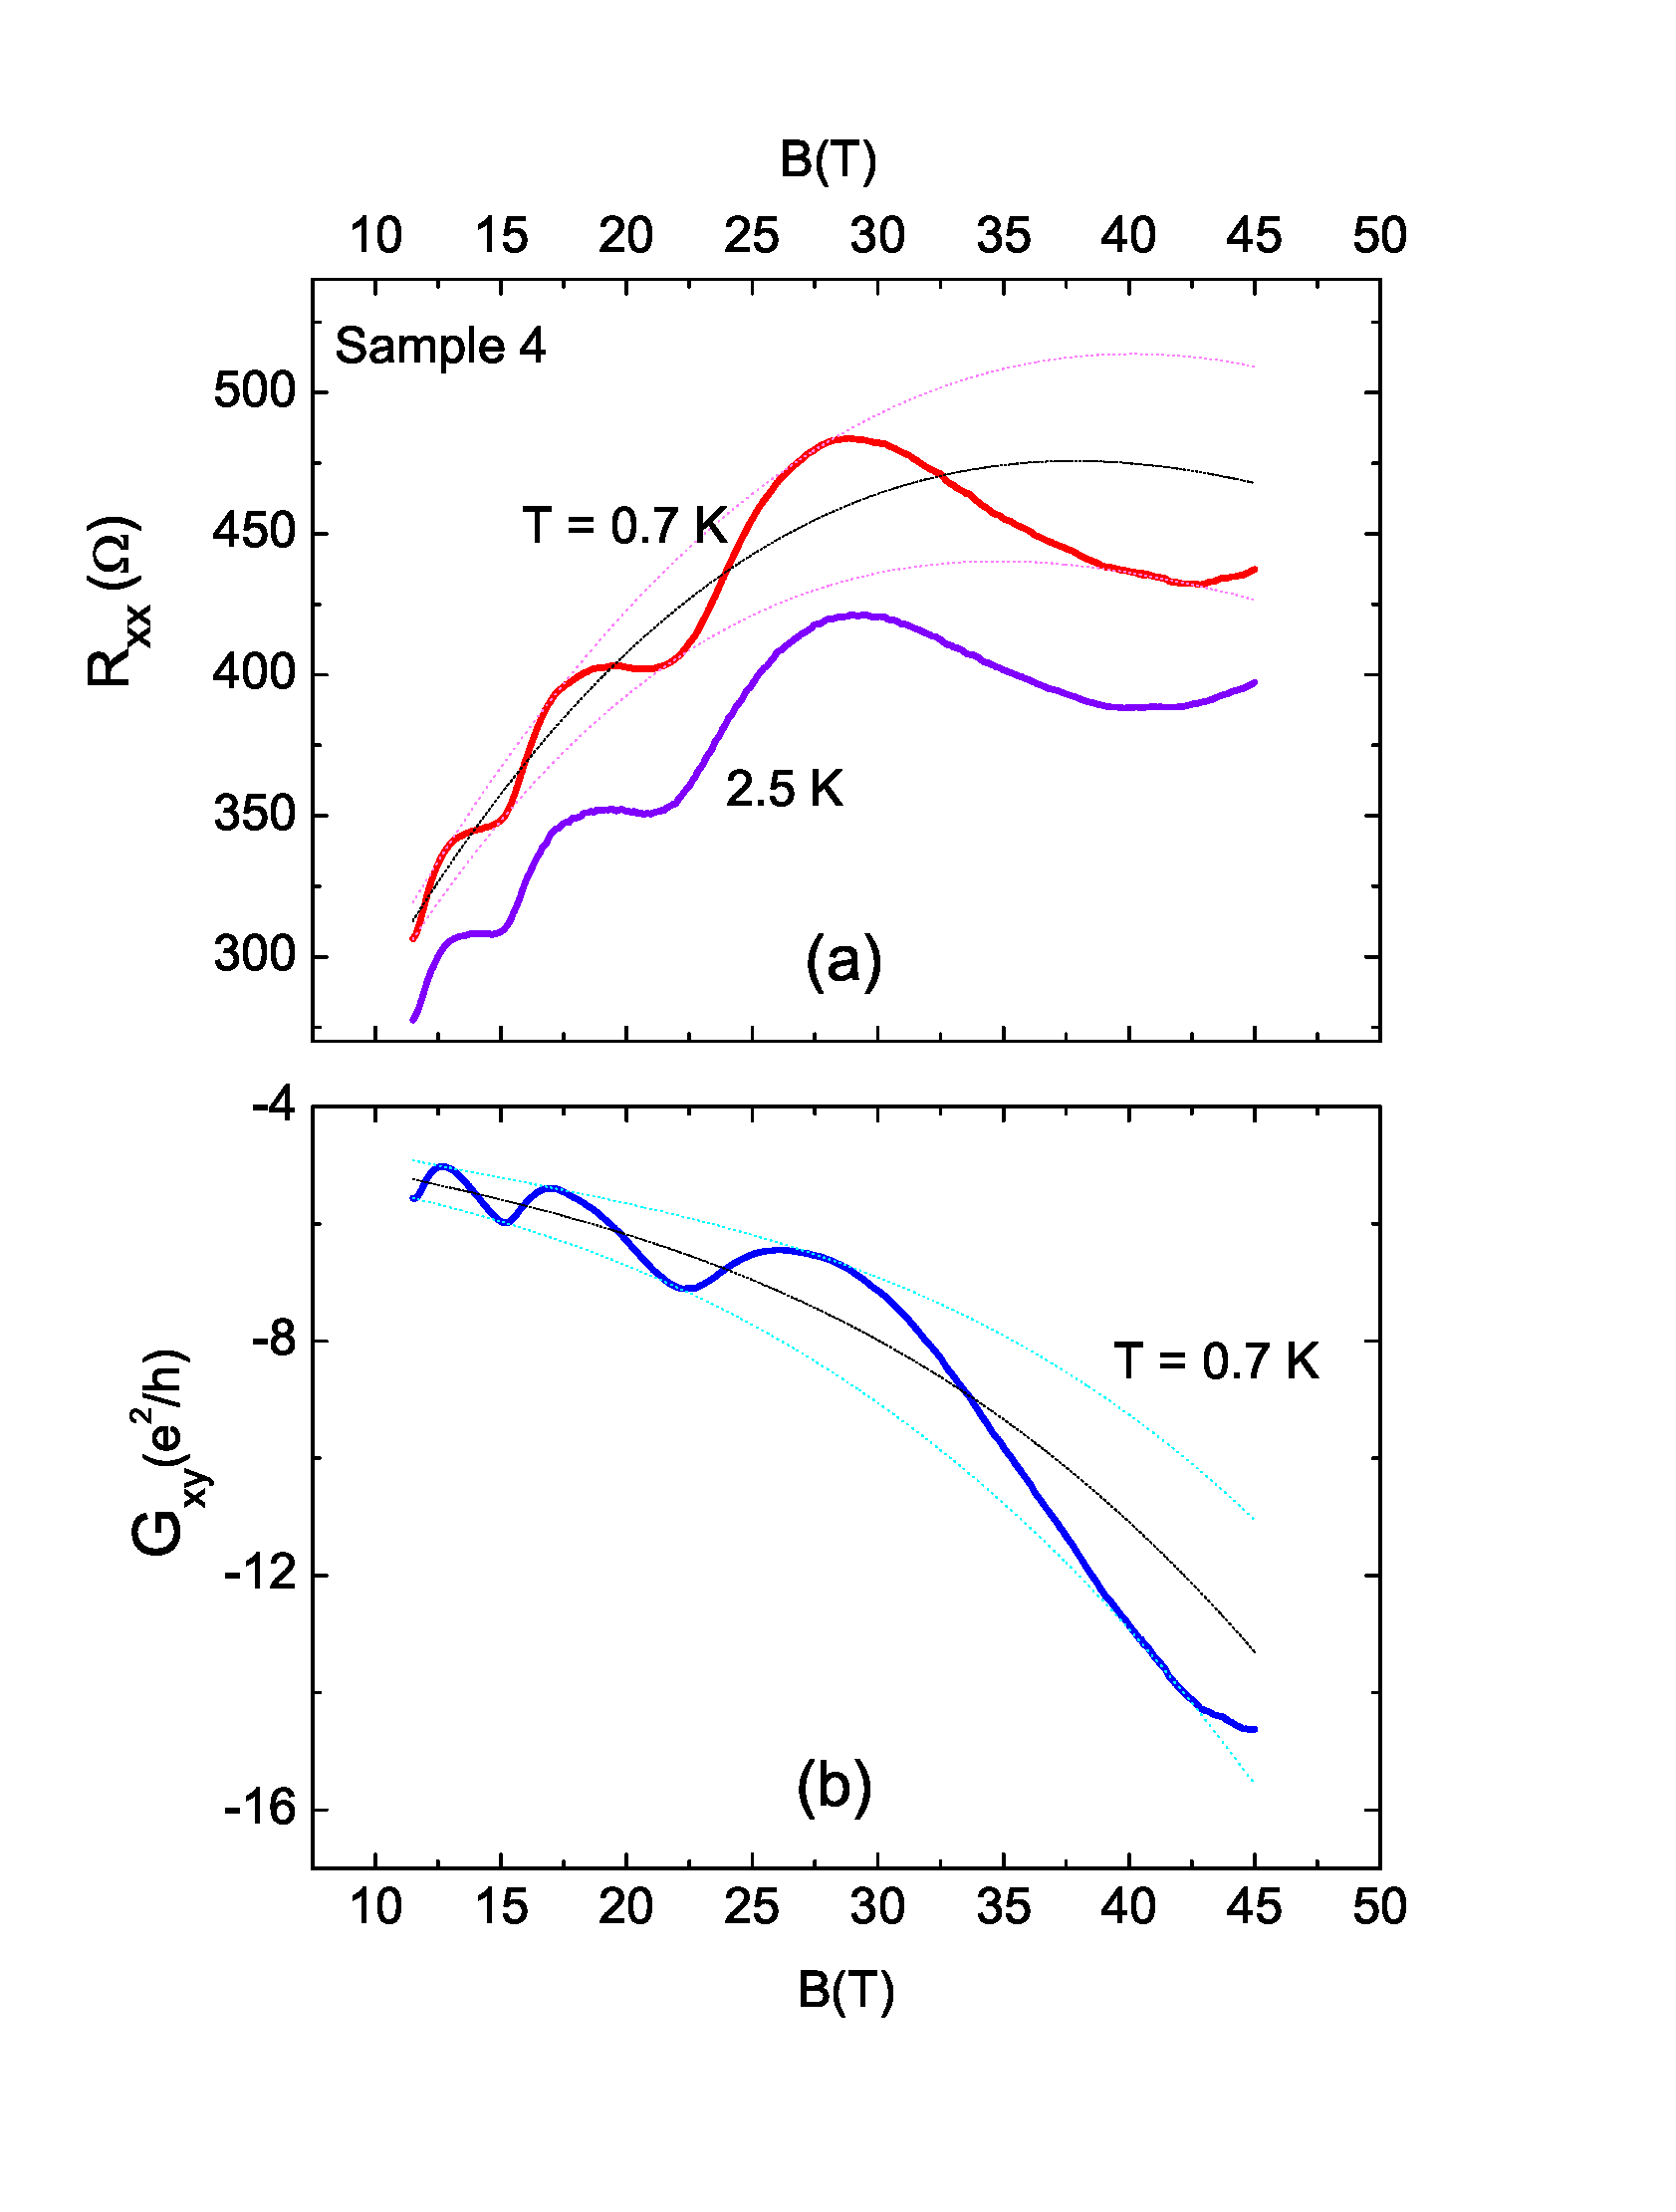
\includegraphics[width=0.9\linewidth]{ch-bts/figures/FigRxxvsB.eps}
\caption{\label{figRvsB} (color online)
The resistance (per square) $R_{xx}$ and Hall conductance $G_{xy}$ in Bi$_2$Te$_2$Se (Sample 4) between 11 T and 45 T .
Panel (a) shows the SdH oscillations in $R_{xx}$ \emph{vs.} $B$ at fields above 11 T at $T$ = 0.7 and 2.5 K respectively.
The oscillation amplitudes are very large and comparable to the total resistance. At 40 T, the peak-to-peak amplitude is 17 $\%$ of the observed resistance.  The Hall conductance $G_{xy}$ at 0.7 K is plotted in Panel (b). In both panels, the envelopes of the oscillations are the smooth dotted curves passing through the extrema points. Leveraging these curves, we can determine the background curve (black curve) as the average of the envelope curves.  
}
  \end{center}
\end{figure}

\subsection{Experimental details}
%After setting up the analysis paradigm, we may discuss the experiment details below.
%As discussed in previous sections, Bi$_2$Se$_3$ has a large amount of $n$-type carriers induced by the overwhelming Se vacancies (electron donors). In contrast, Bi$_2$Te$_3$ are $p$-type as a result of the Te-Bi exchange defects. In the hybrid material Bi$_2$Te$_2$Se, the Se ions occupy the innermost layer in each quintuplet layer. This leads to the charge compensation and it suppresses both vacancy formation and Te-Bi exchange defects. Hence the bulk carriers in Bi$_2$Te$_2$Se could be reduced to as low as $10^{16} cm^{-3}$. 
%
%The large density of Se vacancies (electron donors) in Bi$_2$Se$_3$ leads to an $n$-type semi-metal with
%a sizeable carrier 
%density ($n_b\sim10^{18}$ cm$^{-3}$). By contrast, as-grown crystals of Bi$_2$Te$_3$ are $p$-type because of
%Te-Bi exchange defects. In the hybrid material Bi$_2$Te$_2$Se, the Se ions occupy the innermost
%layer in each quintuplet layer. This appears to suppress both vacancy formation
%and Te-Bi exchange defects. Two groups have found that surface
%SdH oscillations are observed in
%$n$-type crystals with greatly reduced $n_b$~\cite{Ando10,Xiong2012}.


The Bi$_2$Se$_3$ crystals we used in a 45T magnetic field were grown by the same method as those in our 14T experiments. However, even in carefully annealed crystals, there are large variations in their bulk carrier densities and the observed resistivities. Figure \ref{figRvsT} shows traces of $\rho$ \emph{vs.} $T$ for a representative set (Samples 1, 2 and 3). At 4 K, $\rho$ varies from 1 to 6 $\Omega$cm.
Although all these samples exhibit clear SdH oscillations in a high magnetic field, the amplitudes are largest when $\rho > 4\;\Omega$cm at 4 K. 


As in Fig. \ref{figRvsT}, we notice that the Hall coefficient $R_H$ changes from $p$ to $n$ type as $T$ decreases to 56 K. Through our high pressure transport experiments of Bi$_2$Se$_3$~\cite{Luo}, we have found that such Hall behavior results from the thermal activation 
of holes into the bulk valence band across a ``transport'' gap $\Delta_T\sim$ 50 mV. At 4 K, when the itinerant bulk holes are frozen out, the total conductance matrix is the sum of two $n$-type parts, namely
\be
G_{ij} = G^s_{ij} + G^b_{ij}.
\label{eq:G}
\ee
%As discussed in previous sections, the quantum oscillations from the surface conductance $G^s$ indicate a high mobility $\mu_s$ of 2,800 cm$^2$/Vs~\cite{Xiong2012}, whereas the residual bulk carriers (from an impurity band) has a much smaller mobility ($\mu_b\sim$ 50 cm$^2$/Vs). The magnitudes of $G^s$ inferred from $k_F$ and $\mu_s$
%confirm that the SdH oscillations are from surface states. 
%Ando's group has shown in field-tilt experiments that the SdH period is consistent
%with surface states~\cite{Ando10}.
%Helical surface states in an isolated Dirac band have been observed by spin-resolved ARPES~\cite{Suyang}.

We may also understand the variation of $\rho$ by estimating the density of defects. If we assume that each defect (either Se vacancies or Te-Bi exchanges) contributes one carrier, the observed $n_b$ (3$\times 10^{16}$ cm$^{-3}$ in Samples 1 and 2) corresponds to a defect density
of a few parts in $10^5$. It implies that the fluctuation at the $10^{-5}$ level could lead to the variations we encountered. 

Such resistivity fluctuations in samples have created large difficulties for our high field experiments. Since different parts of our optimally annealed crystals could still display different $\rho$-$T$ profiles, as some parts are metallic and some are insulating, it takes a lot of effort to find an insulating sample. In addition, the amplitudes of the surface quantum oscillations are severely decreased as the sample ages (roughly by a factor of 2 over a few weeks even for crystals sealed in Ar atmosphere and stored in dry ice). All these factors have make it difficult for us to measure the surface quantum oscillations in the National High Magnetic Field Laboratory(NHMFL) in Florida. 

In NHMFL, we cleaved crystals $\sim$30 minutes before quickly loading them into the high-field cryostat in order to improve the surface quality. We put 3 pairs of contact leads on each crystal so that the whole resistance tensor $R_{ij}$ can be measured over distinct segments. Because the 45-Tesla field in NHMFL cannot reverse its direction, we employed the reciprocity technique from Ref.~\cite{Sample1987} to obtain the data in the negative fields and extract both $R_{xx}$ and $R_{yx}$. 



%%%%%%%%%%%%%%%%%%%%%%%%%%%%%%%%%%
%%%%%%%%%%%%%%%%%%%%%%%%%%%%%%%%%%
%%%%%%%%%%%%%%%%%%%%%%%%%%%%%%%%%% FIGURE 3
\begin{figure}[!htbp]
  \begin{center}
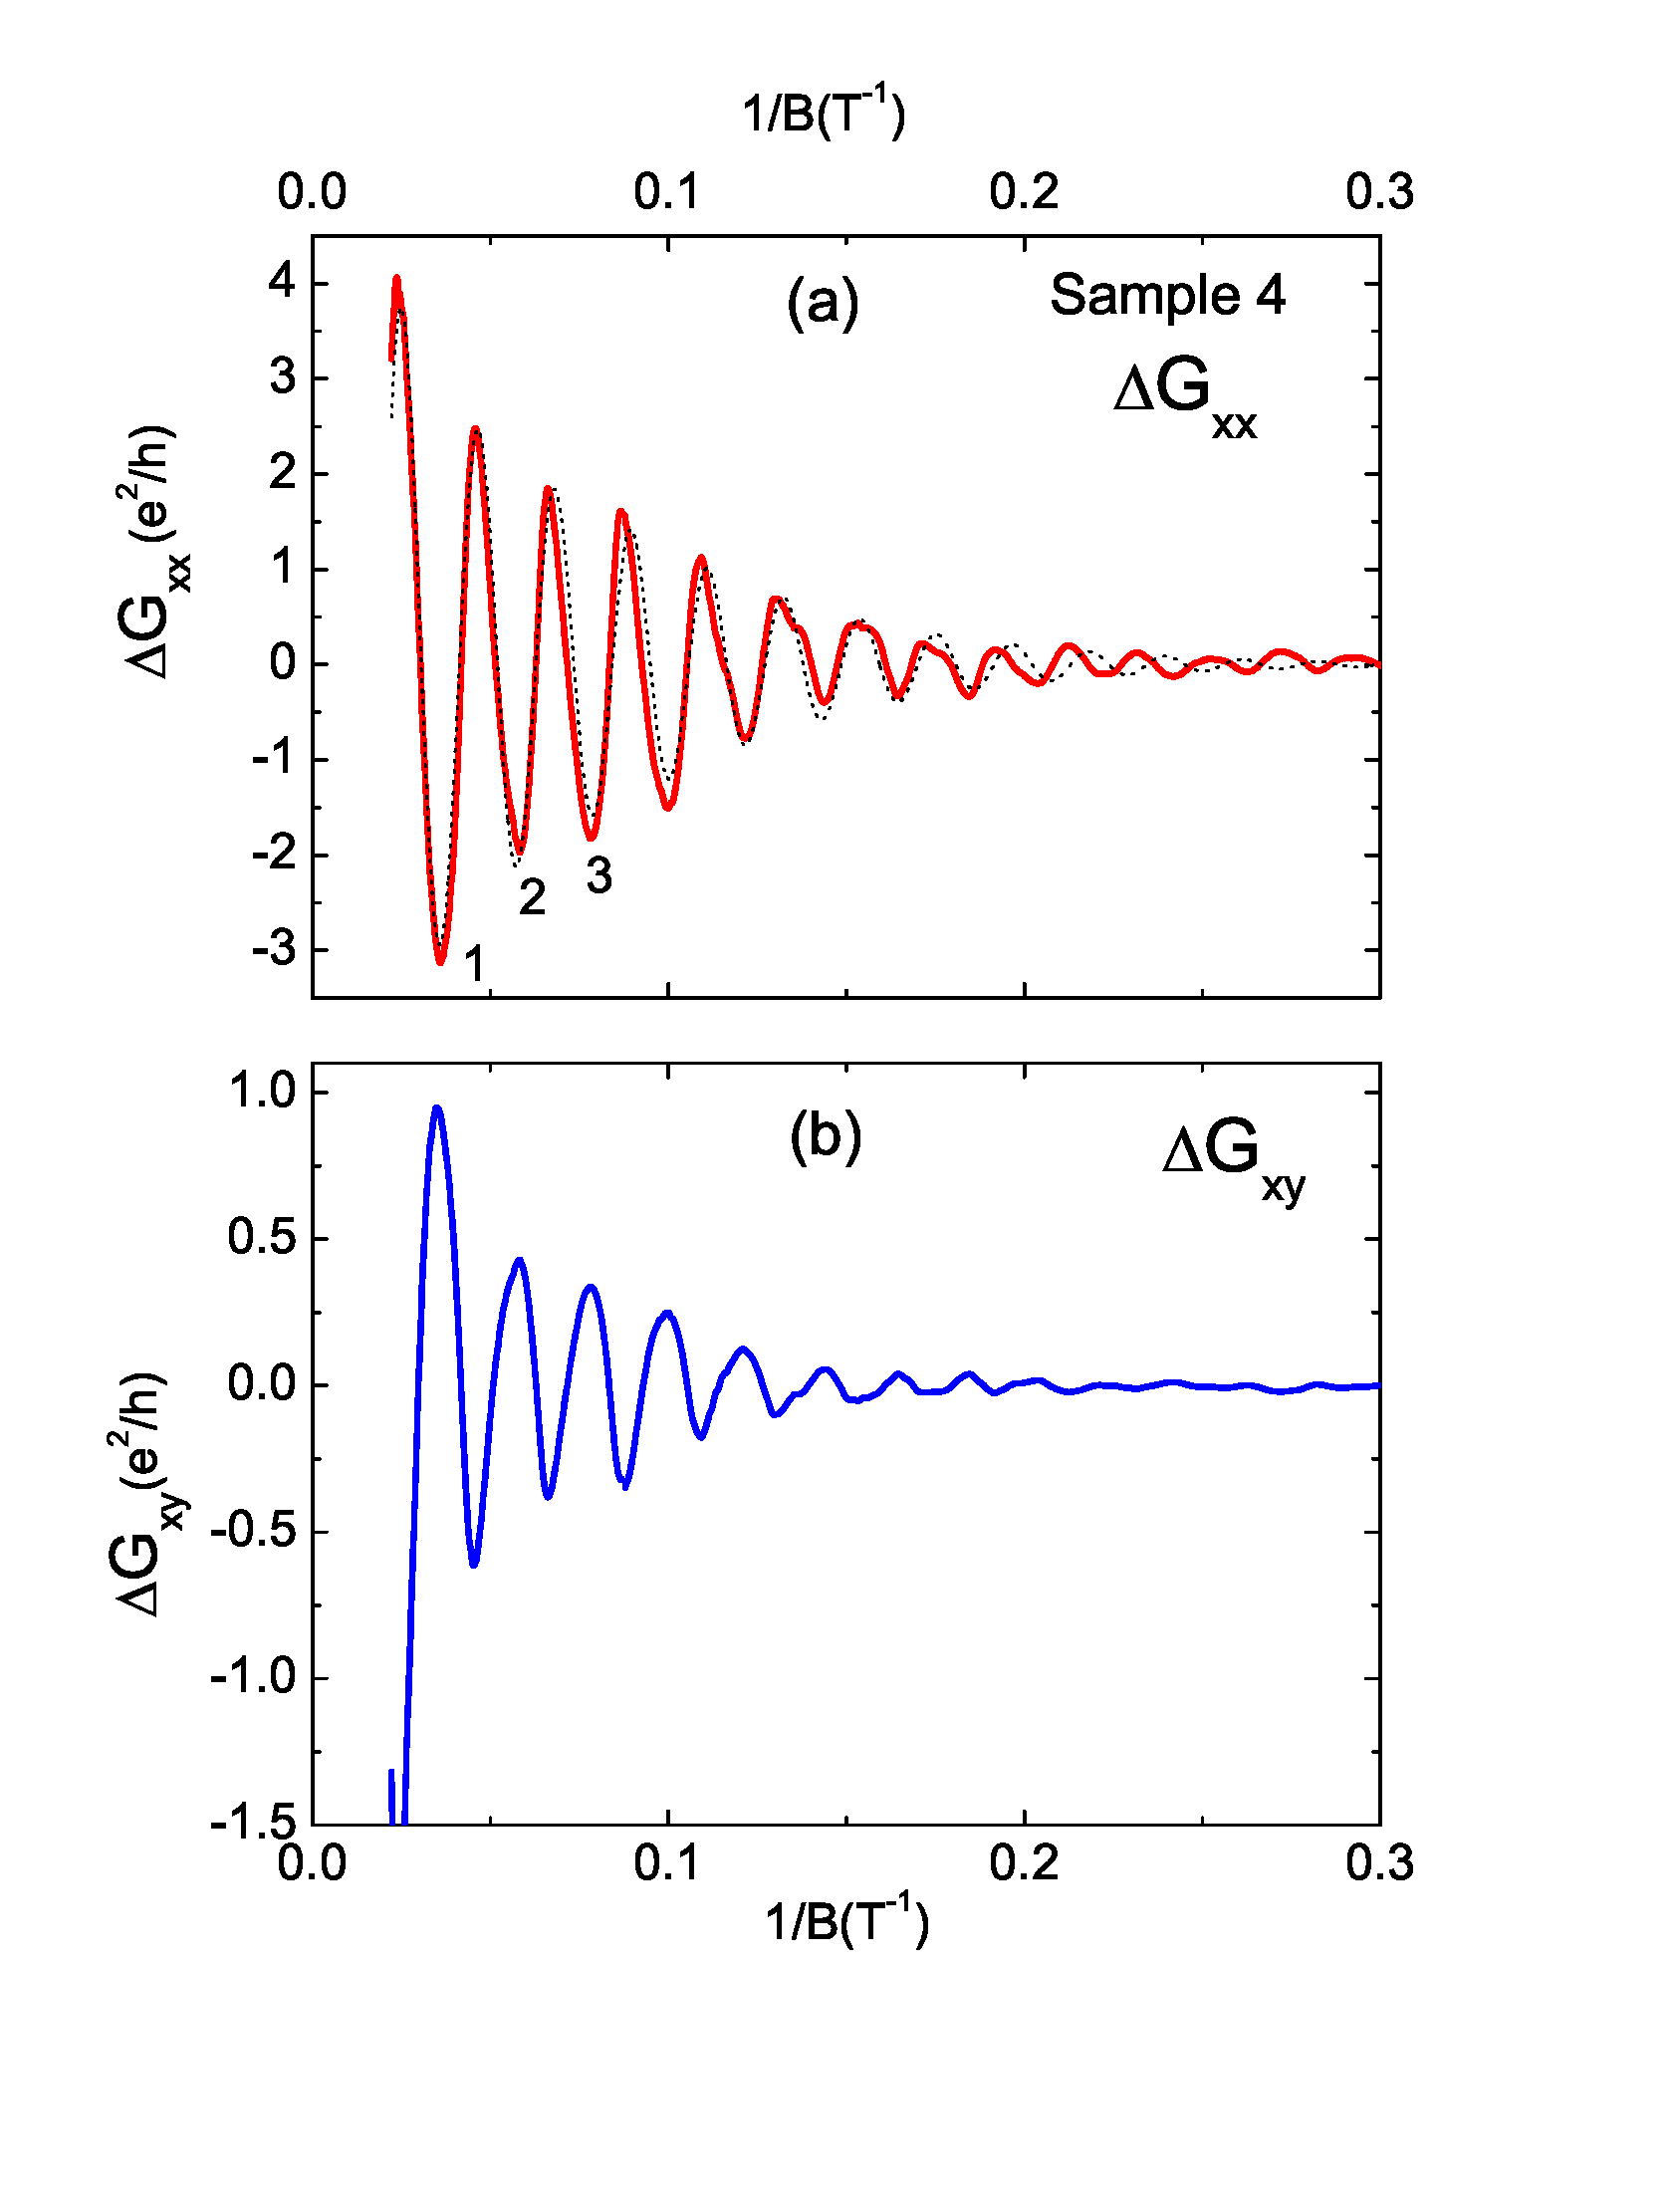
\includegraphics[width=0.8\linewidth]{ch-bts/figures/FigDG.eps}
\caption{\label{figG} (color online)
The oscillatory component of the conductance $\Delta G_{xx}$ (Panel a) and the 
Hall conductance $\Delta G_{xy}$ (Panel b) after a background subtraction in Sample 4 plotted against $1/B$ ($T$ = 0.7 K). The two quantities
are normalized to $e^2/h$. In Panel a, the faint dashed curve is a fit 
to the Lifshitz-Kosevich expression (Eq. \ref{eq:sdh}) using a single frequency. The fit is very good at high field but there is a phase shift at low $B$. The fitting parameters yield a surface mobility of 3,200$\pm$300 cm$^2$/Vs, with $k_F\ell$ = 30. This mobility is higher than that in our 14T experiment. Through the Fermi wavevector $k_F$ and the mobility from the fit, we can calculate $G^s$ in Sample 4 and it accounts for $\sim 19\%$ of the total conductance at 4 K. And at the highest field, the surface state has entered the $n$=1 LL, which could give us a precise measurement of the Berry phase.
The LL indices $n$ = 1,2,3 are indicated for the 
minima of $\Delta G_{xx}$. 
}
  \end{center}
\end{figure}

%%%%%%%%%%%%%%%%%%%%%%%%%%%%%%%%%%
\subsection{Quantum oscillations up to 45T}

The transport measurement results up to 45 T in Samples 1 and 4 are discussed below (in which $R_H$ = -137 and -52 cm$^3$/C, respectively, at 4 K). As shown in Fig. \ref{figRvsB}a, we have observed large and well-resolved SdH oscillations in these samples. Such distinguishable surface quantum oscillations allow us to investigate the interesting problems in the quantum limit with the best accuracy. As displayed in Fig. \ref{figRvsB}a, the peak-to-peak SdH amplitudes in the longitudinal resistance $R_{xx}$ in Sample 4 grows with $B$ and eventually accounts for $\sim$17$\%$ of the total resistance at 45T. Since the oscillations purely come from the surface states, it indicates that the surface contribution is comparable to the bulk current in our samples. To determine $B_n$ accurately, it is appropriate to convert $R_{ij}$ to the conductance matrix by $G_{xx} = R_{xx}/[R_{xx}^2+R_{yx}^2]$ and $G_{xy}= R_{yx}/[R_{xx}^2+R_{yx}^2]$. A display of $G_{xy}$ is in Fig. \ref{figRvsB}b. Then we also need to subtract an appropriate background to isolate the oscillatory part and determine the accurate positions of the \emph{minima} and \emph{maxima} of  $G_{xx}$. We first use a smooth polynomial function to fit the envelope of the oscillations (the faint dashed curves in Fig. \ref{figRvsB}), and then locate the midpoints between the two envelope curves to define the background curve.


After removing the background, we present the oscillatory components $\Delta G_{xx}$ and $\Delta G_{xy}$ versus $1/B$ in Fig. \ref{figG}a and \ref{figG}b respectively (both are normalized to the quantum of conductance $e^2/h$).
In Panel (a), we have also added a fit to the standard Lifshitz-Kosevich expression (Eq. \ref{eq:sdh}) with just
one frequency (dashed curve). The fit is very good at high field but there is a phase shift at low $B$. The fitting parameters yield a surface mobility of 3,200 cm$^2$/Vs and a metallicity parameter $k_F\ell$ = 30. This mobility is higher than that in our 14T experiment. We will discuss the interesting phase shift apparent at low $B$ later.


%%%%%%%%%%%%%%%%%%%%%%%%%%%%%%%%%%
%%%%%%%%%%%%%%%%%%%%%%%%%%%%%%%%%%
%%%%%%%%%%%%%%%%%%%%%%%%%%%%%%%%%% FIGURE 4
\begin{figure}[!htbp]
  \begin{center}
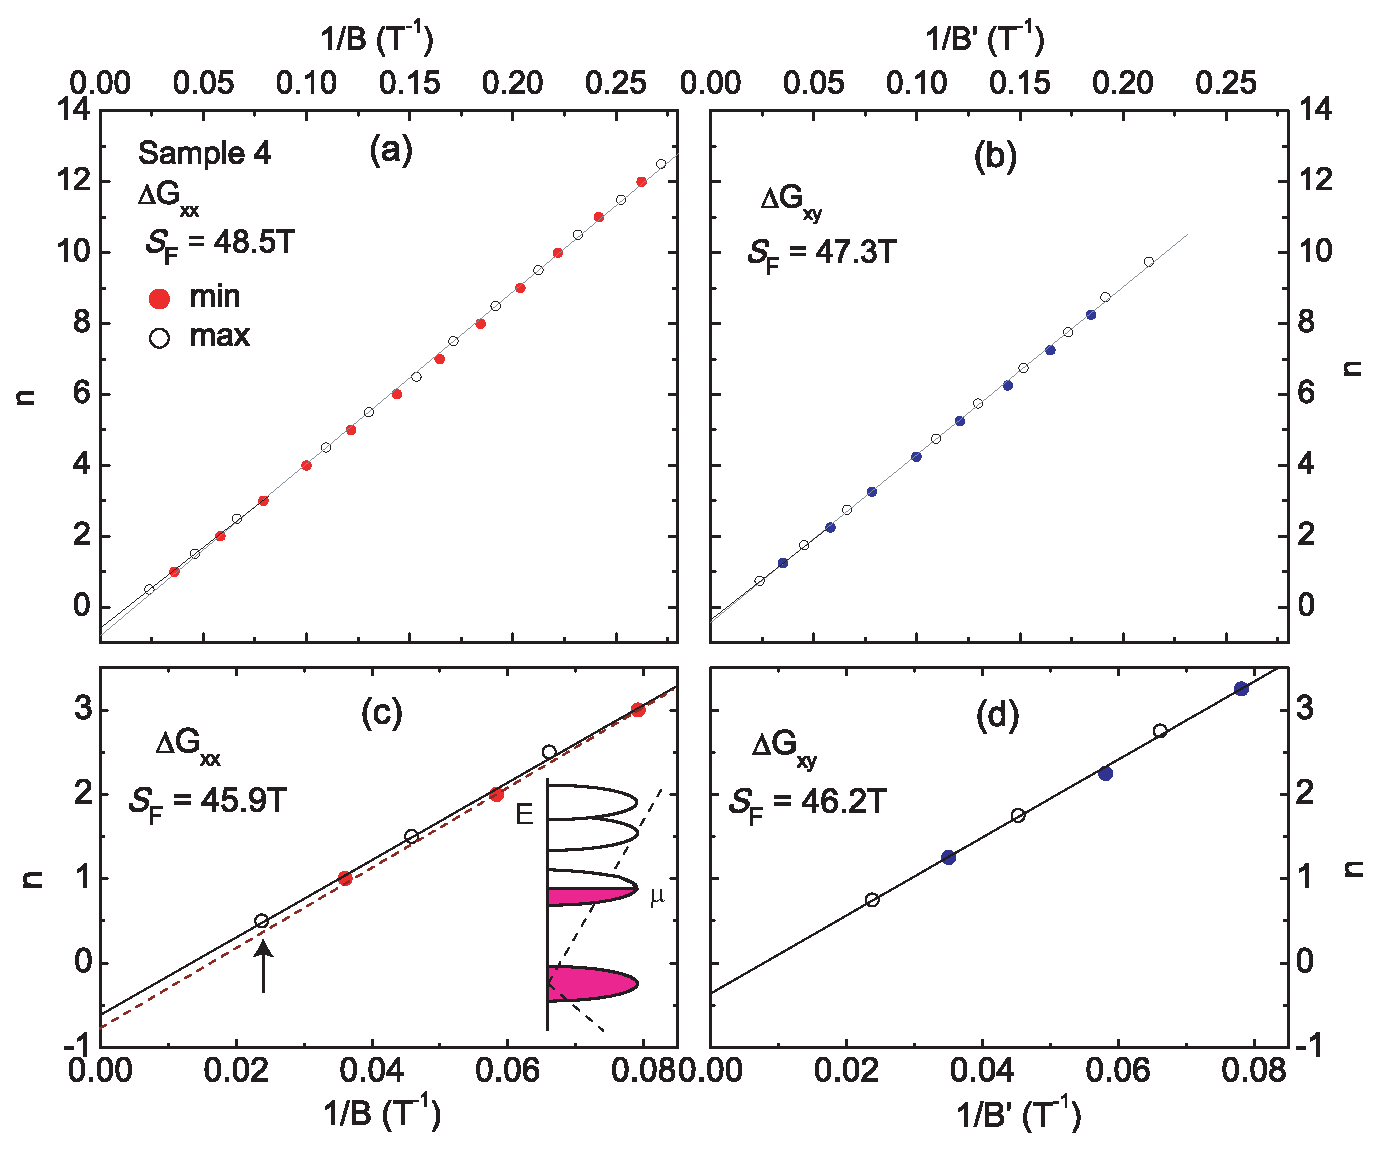
\includegraphics[width=0.9\linewidth]{ch-bts/figures/FigIndexAll4.eps}
\caption{\label{figindex} (color online)
The index plots of $1/B_n$ \emph{vs.} the integers $n$ in Sample 4. In Panel (a), $B_n$ is obtained from
the minima of $\Delta G_{xx}$. In Panel (b), the index field $B'_n$ is inferred from the minima of
$-\Delta G_{xy}$. $B'_n$ is plotted against $n+\frac14$, where the $\frac14$ shift arises because 
the minima in $d\Delta G_{xy}/dB$
align with the minima in $\Delta G_{xx}$. We expand the scale in Panels (c) and (d) to
show the intercepts more clearly. 
In Panel (c), the solid straight line is the best fit to the extrema fields for $n\le$3. The
dashed line is the best fit to all the extrema field shown in Panel (a).
The sketch shows the chemical potential $\mu$ in relation to the filled LLs (solid color) in the Dirac spectrum when
$B$ = 42.0 T (arrow). 
}
  \end{center}
\end{figure}

%%%%%%%%%%%%%%%%%%%%%%%%%%%%%%%%%%

Then we can use our above criteria to determine $B_n$, and Figure \ref{figindex}a exhibits the minima 
of $\Delta G_{xx}$ versus $n$ (solid circles) of Sample 4. In addition, the maxima of $\Delta G_{xx}$ have been plotted as open circles (shifted by $\frac12$) and they correspond to $n+\frac12$. The slope of the fitted straight line gives a Fermi cross-section area $S_F$ of 48.5 T.
A similar plot based on the extrema of the Hall conductance $\Delta G_{xy}$ 
is shown in Fig. \ref{figindex}b. As in the quantum Hall system, the $G_{xy}$ and $G_{xx}$ extrema have a $\frac{\pi}{2}$ phase difference, and thus the minima in $-\Delta G_{xy}$ correspond to $n+\frac14$.The Fermi surface area $S_F$ found from $\Delta G_{xy}$ (47.3 T) is consistent with the value from  $\Delta G_{xx}$ within our resolution. We also note the values of $n$ = 1,2,3 at the minima of $\Delta G_{xx}$ in Fig. \ref{figG}a.


In order to have a clear view of the intercept $\gamma$, we expand the scale in Fig. \ref{figindex}c. The best-fit straight line passing through the six extrema of $\Delta G_{xx}$ intercepts the $n$-axis at the value $\gamma$ = -0.61$\pm$0.03. Similarly, the high-field
extrema of $\Delta G_{xy}$ and their fitted line are presented in Fig. \ref{figindex}d. The intercept occurs at $\gamma$ = -0.37$\pm$0.03. Within our uncertainties, both values are significantly closer to the theoretical value $\gamma=-\frac12$ than 0 or 1. Also, our samples have already entered the $n=\frac12$ Landau level, it is significantly closer to the limit $1/B\to 0$ than previous experiments. As a result, it can also give a better resolution in determining the intercept $\gamma$. Hence, the high-field results we present here provide clear transport evidence for a Dirac spectrum of the surface states on Bi$_2$Te$_2$Se.

Another interesting thing is the large amplitudes of the quantum oscillations. Although we have not observed any quantized Hall steps in Fig. \ref{figG}b (the oscillatory component that we extract by subtracting a smooth background from the bulk states), we find that the peak-to-peak
amplitude of $\Delta G_{xy}$ at $n=1$ is $\sim$0.8 $e^2/h$ per surface, which is of the order
of the quantized Hall conductance value.

In Sample 1, the amplitudes of the observed SdH oscillations are considerably
weaker (Fig. \ref{figG1}a) than those of Sample 4. But it also enters the $n=1$ Landau level at the highest field. The fitted straight line to the $1/B_n$ vs. $n$ plot also intercepts the $n$-axis at $\gamma$ = -0.45$\pm$0.02, confirming a Dirac spectrum in Sample 1's surface states.

In the expanded plot Fig. \ref{figindex}c we show why the high fields are necessary to find $\gamma$ accurately. At a field as high as 45T, we can access the very low Landau index as $n=\frac12$ in Figs. \ref{figindex}c and d. Thus the bias and uncertainty that the fitted intercept can have is reduced considerably because it is almost fixed by the experimental data at $n=\frac12$. In our data, an intercept $\gamma = 0$ can be safely excluded as the allowed error from our fit is small. A more subtle point is the slight curvature of the index plot. In Fig. \ref{figindex}c, if we extrapolate the best-fit line (dashed) using the total data set from 3 to 45 T, its intercept yields -0.78, nearly exactly between -1 and
-$\frac12$. In comparison, the best-fit line (bold) to the high-field extrema
for $n\le$3 yields an intercept (-0.61) closer to -$\frac12$. This difference implies that the index curve
$1/B_n$ vs. $n$ develops a slight curvature over the large field range. And as we may notice in Fig. \ref{figG}a, this curvature may also appear as a phase shift at different fields when it is compared to the single-frequency fit. 


%%%%%%%%%%%%%%%%%%%%%%%%%%%%%%%%%%
%%%%%%%%%%%%%%%%%%%%%%%%%%%%%%%%%%
%%%%%%%%%%%%%%%%%%%%%%%%%%%%%%%%%% FIGURE 5
\begin{figure}[!htbp]
  \begin{center}
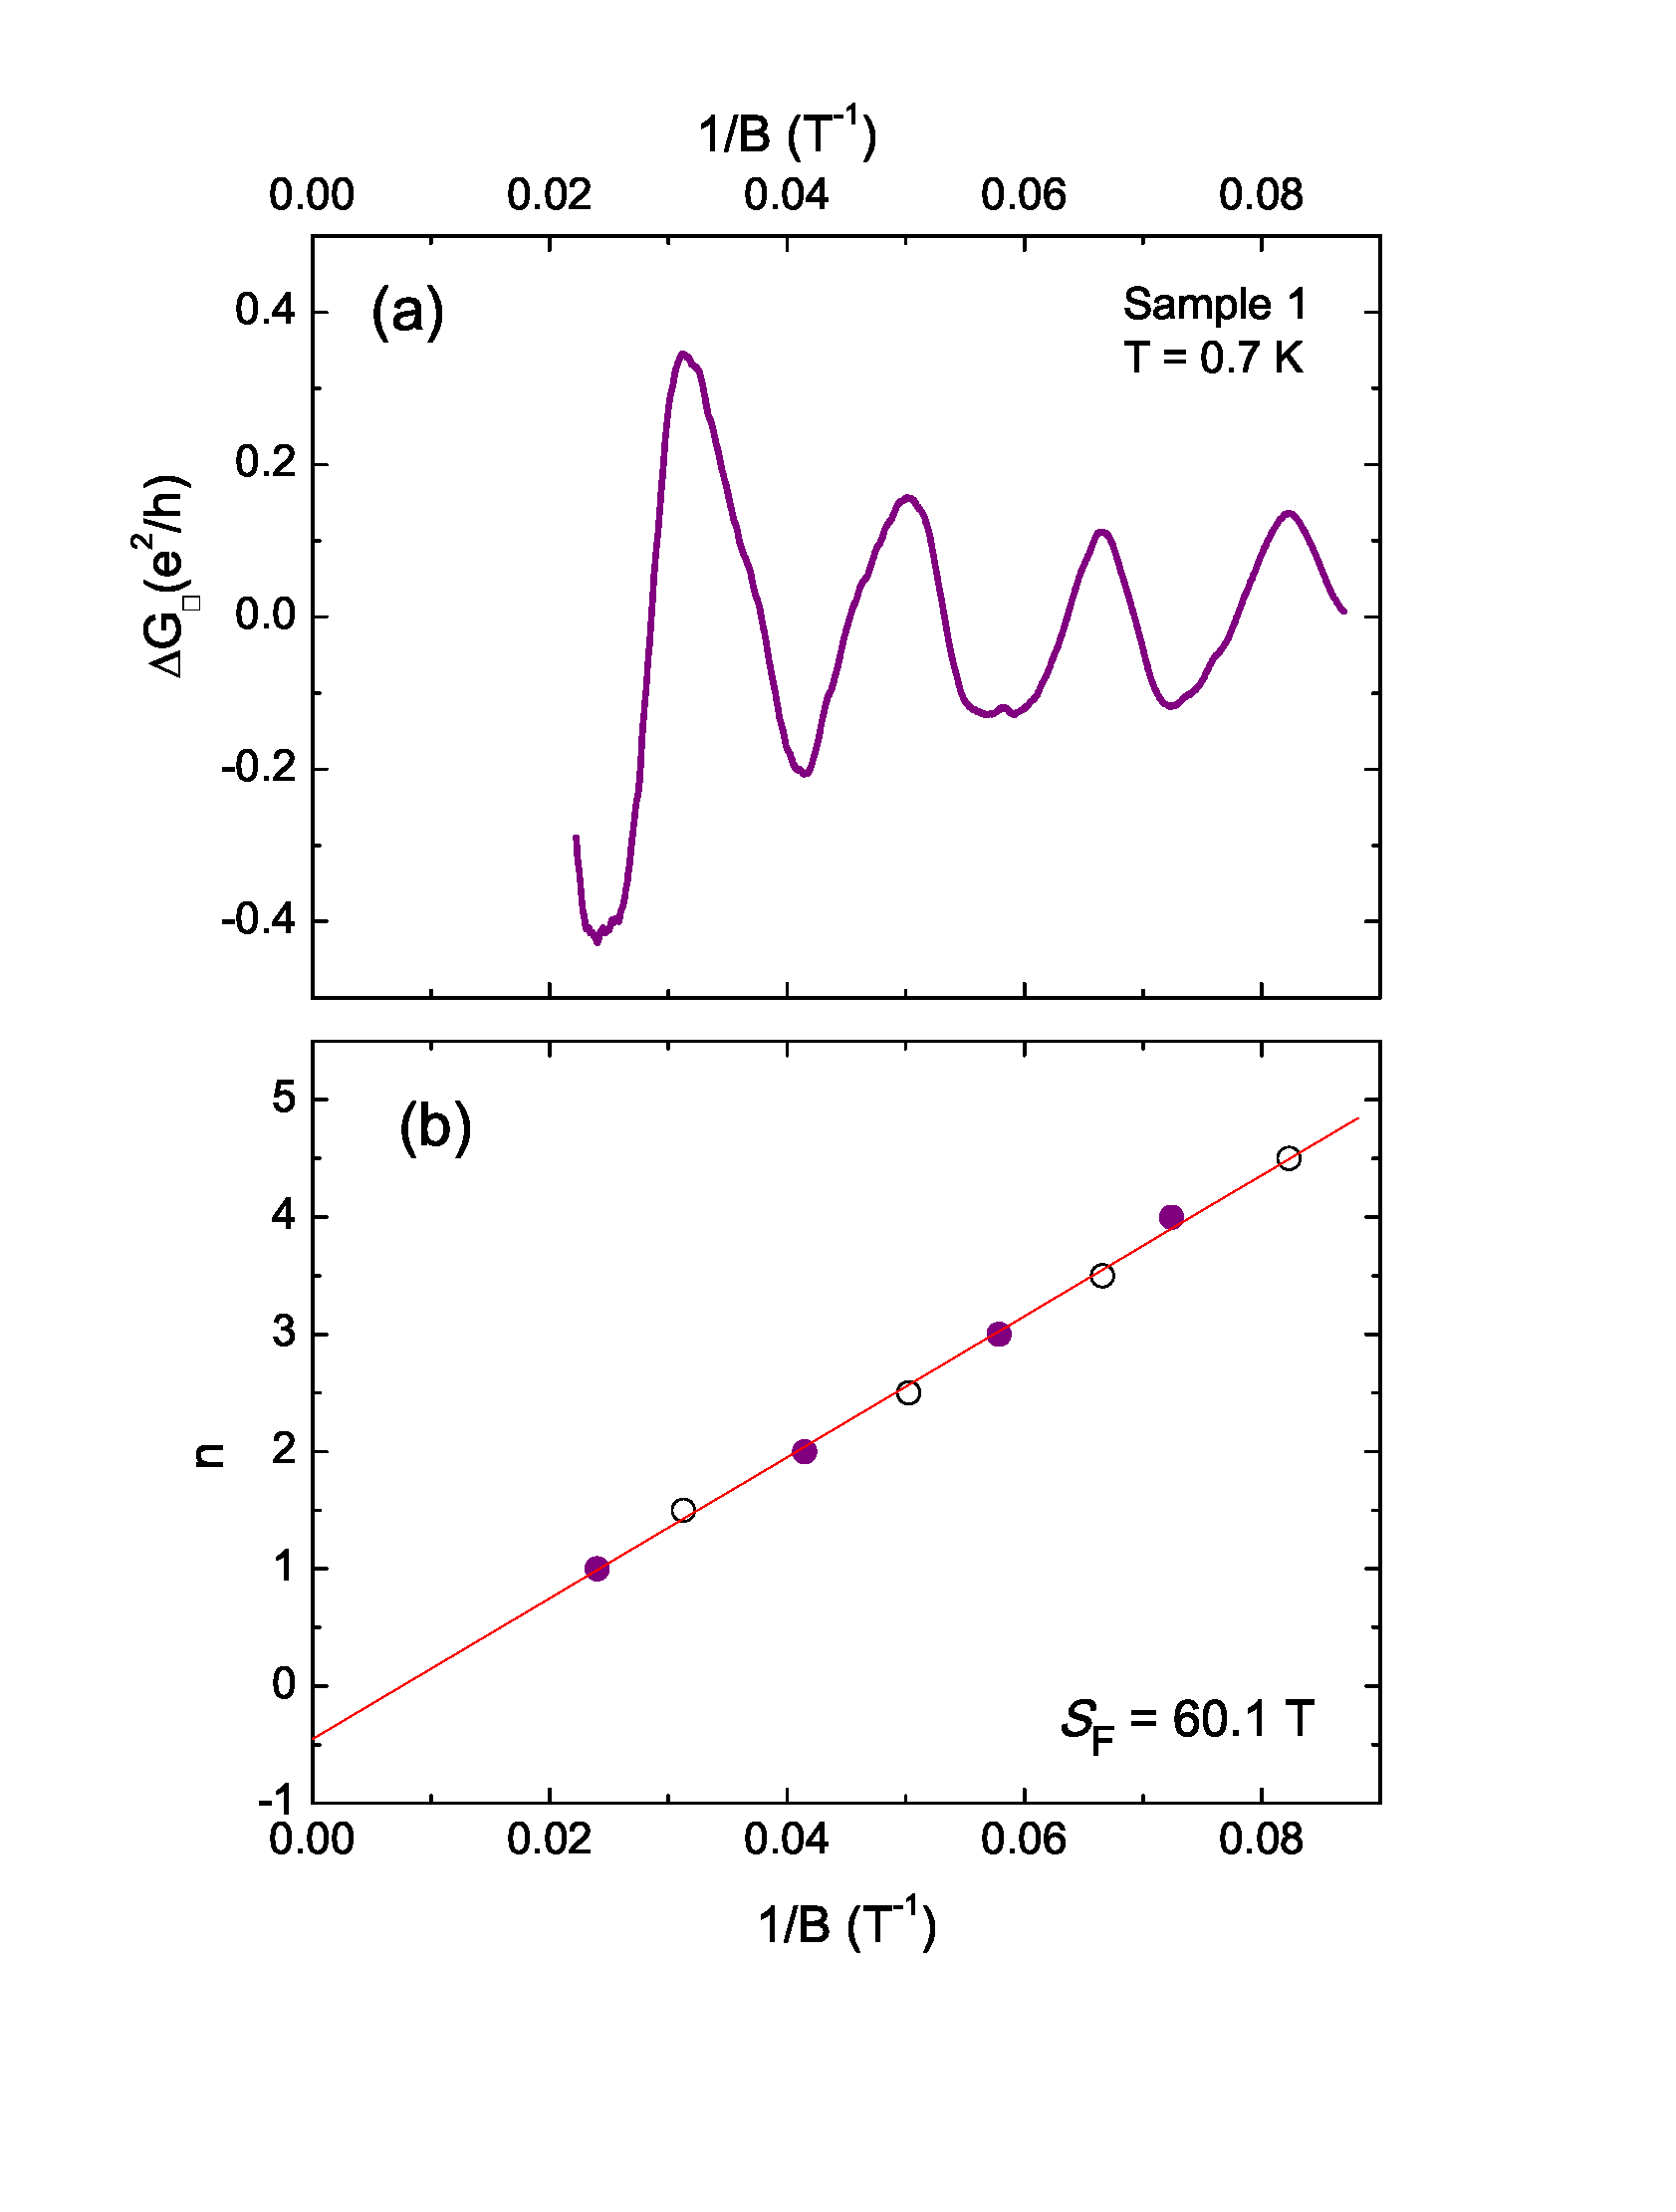
\includegraphics[width=0.9\linewidth]{ch-bts/figures/FigGindexS1.eps}
\caption{\label{figG1} 
The oscillatory component $\Delta G_{xx}$ vs. $1/B$ (Panel a) and the 
index plot of $1/B_n$ vs. $n$ (Panel b) in Sample 1. The intercept $\gamma$ of the best-fit line 
is -0.45$\pm$0.02.}
  \end{center}
\end{figure}

%%%%%%%%%%%%%%%%%%%%%%%%%%%%%%%%%%
%A second issue we address is the strength of the Zeeman energy.
%Strict particle-hole symmetry implies that it is unshifted in energy. 
%On the other hand, a large Zeeman energy $g\mu_BB$ may lead to high-field distortion of the
%SdH period ($g$ is the surface Lande g-factor
%and $\mu_B$ the Bohr magneton).
%The in-field STM experiments ~\cite{Hanaguri,Xue10} have shown that the $n$ = 0 LL is unshifted up to 11 Tesla. 
%This test can be extended to much larger $B$ in transport experiments, but early SdH experiments had limited
%resolution~\cite{Qu,Analytis}. Values of $g$ as large as 76 have been inferred from low-field
%SdH oscillations in Bi$_2$Te$_2$Se~\cite{Taskin}.

As discussed above, the Zeeman energy could possibly cause a curvature in the index plot. When the Zeeman term is included, the Hamiltonian is
\be
H = v_F {\bf \hat{n}}\cdot \bm{\sigma\times\pi}- \frac{g\mu_B}{2} {\bf B}\cdot\bm{\sigma}
\label{eq:H}
\ee
where $\bf \hat{n}$ is the unit vector normal to the surface. $\bm\sigma$ are the spin Pauli matrices, and $\bm{\pi} = {\bf p}-e{\bf A}$ is the momentum $\bf p$ of the
electron in a vector potential ${\bf A}$. The LL energy is given by 
\be 
E_n = \pm\sqrt{2n\hbar v_F^2 eB + (g\mu_B B/2)^2}.
\label{eq:En}
\ee
In contrast to the case without Zeeman energy, the energy of the $n=0$ LL increases linearly with $B$ instead of being unshifted.
For a large $g$-factor, the $1/B_n$ vs. $n$ curve will deviate from a straight line as $1/B\to$ 0. However, in our experiment, we have
tracked the LLs to $n$ = 1. The weak deviation from a straight line in Fig. \ref{figindex}c) 
is inconsistent with values of $g$ substantially larger than 2. More importantly, the
observed curvature is opposite in sign to that predicted by Eq. \ref{eq:En}. Since there is no significant deviation in our data that could be explained by the Zeeman energy, we conclude that the 
the $g$ factor of the surface states in Bi$_2$Te$_2$Se is not significantly greater than 2 in the quantum limit. 

\subsection{Surface carrier mobility}\label{fit}

In most of the Bi-based topological compounds, it is very difficult to separate $G^s$ from $G^b$ reliably.  
But Shubnikov de-Haas (SdH) oscillations -- when measured with a high resolution -- 
provide a powerful way to isolate the surface conductance.
The period of the oscillations yields the Fermi surface area and thus the Fermi wavevector $k_F$. The surface mobility and the scattering rate can also be obtained by fitting the field dependence of the SdH amplitudes.
Then we can obtain the zero-field value of $G^s_{xx}\equiv G^s$ using
\be
G^s = (e^2/h)k_F\ell.
\label{eq:Gs}
\ee

To isolate the surface quantum oscillations, we first use a smooth polynomial function to simulate the envelope curves
passing through the extrema of the oscillations on the raw data curves as explained above. The background is defined as the midpoints of the two envelope curves. Then we obtain the oscillatory component $\Delta G_{xx}$ by subtracting the background from $G_{xx}$. We also notice that  $\Delta G_{xx}$ may not account for all of the
surface conductance, because its field-averaged value $\langle\Delta G_{xx}\rangle_B$
vanishes while $G^s_{xx}$ should have some field dependence. Hence we conclude that $\Delta G_{xx}$ is smaller than $G^s_{xx}$.



%%%%%%%%%%%%%%%%%%%%%%%%%%%%%%%%%%%%%%%%
%%%%%%%%%%%%%%%%%%%%%%%%%%%%%%%%%%%%%%%%
%%%%%%%%%%%%%%%%%%%%%%%%%%%%%%%%%%%%%%%%
%%%%%%%%%%%%%%%%%%%%%%%%%%%%%%%%%%%%%%%% FIGURE 6

\begin{figure}[!htbp]
  \begin{center}   
\incl[width=0.9\linewidth]{ch-bts/figures/FigGfit.eps} 
\caption{\label{figfit} 
The oscillatory component of the conductance $\Delta G_{xx}$ in Sample 4 at 0.7 K
(solid curve) and the fit to Eq. \ref{eq:sdh} using only one frequency (dashed curve). 
}
  \end{center}
\efig

Then we leveraged the standard Lifshitz-Kosevich expression~\cite{Roth} to fit the oscillatory component $\Delta G_{xx}$. The formula is:
\be
\frac{\Delta G_{xx}}{G_{xx}} = \left(\frac{\hbar\omega_c}{2E_F}\right)^{\frac12}
\frac{\lambda}{\sinh\lambda} e^{-\lambda_D}\cos
\left[\frac{2\pi E_F}{\hbar\omega_c}+\varphi\right],
\label{eq:sdh}
\ee
%with $\lambda = 2\pi^2k_BT/\hbar\omega_c$ and $\lambda_D = 2\pi^2k_BT_D/\hbar\omega_c$,
%where $\omega_c$ is the cyclotron frequency and 
%the Dingle temperature is given by $T_D = \hbar/(2\pi k_B\tau)$,
%with $\tau$ the lifetime. For 2D Dirac electrons, the SdH frequency is determined by the chemical potential as
%$2\pi E_FB/(\hbar\omega_c)$, which simplifies to $4\pi^2\hbar n_s/e$, with the 2D
%carrier density $n_s = k_F^2/4\pi$ (per spin).  
%In equation \ref{eq:sdh}, the cyclotron mass for a Dirac system is given by $m_c = E/v_F^2$.  
The formula is almost the same as Eq. \ref{eq:sdh_hall} except that the phase $\varphi$ here is shifted by $\frac{\pi}{2}$ from that of the Hall conductivity. 


As displayed in Fig. \ref{figfit}, with one Fermi pocket, we have already obtained a very good fit (dashed line) to the observed oscillations (bold curve). The three fitting parameters are $k_F$ = 0.038 \AA$^{-1}$, $\varphi$ = 0.65$\pi$ and
$T_D$ = 8.5$\pm$1.5 K. They imply a surface 
mean-free-path $\ell$ = 79$\pm$8 nm and mobility $\mu_s = e\ell/\hbar k_F$ = 3,200$\pm$300 cm$^2$/Vs.
The metallicity parameter $k_F\ell$ equals 30. 
These parameters indicate that, in Sample 4 at $B$=0, $G^s$ accounts for $\sim 19\%$ of the
total observed conductance.
The parameters here are also similar to those obtained from our earlier
sample in the 14T experiment, which had a slightly larger $k_F$ (0.047 \AA$^{-1}$)~\cite{Xiong2012}. 


Again, the mobility from the SdH oscillations provides a strong, quantitative argument that the SdH oscillations
origin from surface states. Otherwise if the oscillations arise 
from the bulk states, the SdH period gives a 3D Fermi sphere 
of radius $k_F$ = 0.038 \AA$^{-1}$, or equivalently a 3D carrier density of 1.86$\times 10^{18}$ cm$^{-3}$.  With
this density and the mobility inferred by the Lifshitz-Kosevich formula Eq. \ref{eq:sdh}, we can obtain a 3D resistivity $\rho_b \sim$ 1.1 m$\Omega$cm at 4 K. Instead our measured $\rho$ is around 5 $\Omega$cm, a factor of 4,500 different from the 3D one. Such a large difference eliminates the possibility of the bulk origin of the quantum oscillations.


%\subsection{Discussions}
%
%Many non-trivial properties of the Dirac-like topological surface states have been investigated by the surface sensitive ARPES and STM experiments. Here we showed that these surface states may also display interesting physics for the transport experiments at high magnetic fields. Although the large amount of bulk carriers may overwhelm the fragile surface states on TI, with the appropriate charge compensation method and a high magnetic field, we can use the powerful SdH oscillations to identify the surface conductance and explore the surface states' properties such as $k_F\ell$ and the mobility. With a magnetic field up to 45T, our Bi$_2$Te$_2$Se samples could access $n$=1 or lower Landau levels, providing an accurate determination of the intercept $\gamma$. The intercept we obtained by linearly fitting the Landau index plot $n$ versus $1/B_n$ is close to $-\frac12$. It corresponds to a non-trivial $\pi$ Berry phase expected for the Dirac dispersion of the surface states on TI.  
%
%We also hope to emphasize that the appropriate definition of $B_n$ should be applied to exclude any mistakes in identifying $\gamma$. As explained in the above sections, $B_n$ should be identified with minima in $G_{xx}$ or maxima in $R_{xx}$ when the bulk conductance dominate. In fact it is very tempting to isolate oscillatory $\Delta R_{xx}$ by subtracting a smooth background and then assign integer indices to the minima of the $\Delta R_{xx}$. Nevertheless, this way will result in an opposite and wrong definition of the index. Then it will yield a fake $\frac12$-shift in the intercept even for Schr\"{o}dinger electrons. Furthermore it needs a low index to significantly reduce the uncertainties in fixing $\gamma$. An index plot with many but large indices may still have a large error bar in determining $\gamma$ as the curvature in the plot could easily change the intercept obtained by extrapolation. 
%
%The linearity of the index plot in Figs. \ref{figindex} and \ref{figG1} show that the Lande
%$g$-factor can not be large ($g\sim$2). The $n$ = 0 LL is unshifted even at 45 T, consistent with 
%STM experiments taken at 11 T~\cite{Hanaguri,Xue10}.
%
%Finally, we hope to add some comments on the results in the large-$B$ limit.
%In Fig. \ref{figG}a, the last maximum in $\Delta G_{xx}$ (at $B\simeq$ 40 T) corresponds to
%$n$ = $\frac12$ (see arrow in the index plot in Fig. \ref{figindex}c). At this field, the
%Fermi energy $E_F$ is aligned with the center of the $n$ = 1 LL, as sketched in the
%inset in Fig. \ref{figindex}c. According to our indexing scheme, it means that there are two half-filled
%LLs between $E_F$ and the Dirac Point, with $\frac12$ of the $n=1$ Landau level and $\frac12$ 
%from the unshifted LL at the Dirac Point. Since there are not many LLs between $E_F$ and the Dirac point, our high-field results provide 
%rather firm evidence 
%for this $\frac12$-shift in the limit $1/B\to 0$. 
%As the inset in Fig. \ref{figindex}c implies, we may be able to reach the interesting
%states in the $n$ = 0 LL in Bi$_2$Te$_2$Se in fields higher than 45 T. 

\section{Discussions and Summary}
\label{sec:bts:summary}


Many non-trivial properties of the Dirac-like topological surface states have been investigated by the surface sensitive ARPES and STM experiments. Although the large amount of bulk carriers may overwhelm the fragile surface states on many TIs, here we found a TI crystal with a large bulk resistivity with the appropriate charge compensation method. The suppressed bulk conductance has enabled us to measure the surface states of Bi$_2$Te$_2$Se directly in a transport experiment. We showed that these surface states on Bi$_2$Te$_2$Se may also display interesting physics for the transport experiments at high magnetic fields. We can use the powerful SdH oscillations to identify the surface conductance and explore the surface states' properties such as $k_F\ell$ and the mobility. With a magnetic field up to 45T, our Bi$_2$Te$_2$Se samples could access $n$=1 or lower Landau levels, providing an accurate determination of the intercept $\gamma$. The intercept we obtained by linearly fitting the Landau index plot $n$ versus $1/B_n$ is close to $-\frac12$. It corresponds to a non-trivial $\pi$ Berry phase expected for the Dirac dispersion of the surface states on TI.  

We also hope to emphasize that the appropriate definition of $B_n$ should be applied to exclude any mistakes in identifying $\gamma$. As explained in the above sections, $B_n$ should be identified with minima in $G_{xx}$ or maxima in $R_{xx}$ when the bulk conductance dominate. In fact it is very tempting to isolate oscillatory $\Delta R_{xx}$ by subtracting a smooth background and then assign integer indices to the minima of the $\Delta R_{xx}$. Nevertheless, this way will result in an opposite and wrong definition of the index. Then it will yield a fake $\frac12$-shift in the intercept even for Schr\"{o}dinger electrons. Furthermore it needs a low index to significantly reduce the uncertainties in fixing $\gamma$. An index plot with many but large indices may still have a large error bar in determining $\gamma$ as the curvature in the plot could easily change the intercept obtained by extrapolation. 

The linearity of the index plot in Figs. \ref{figindex} and \ref{figG1} show that the Lande
$g$-factor can not be large ($g\sim$2). The $n$ = 0 LL is unshifted even at 45 T, consistent with 
STM experiments taken at 11 T~\cite{Hanaguri,Xue10}.

Finally, we hope to add some comments on the results in the large-$B$ limit.
In Fig. \ref{figG}a, the last maximum in $\Delta G_{xx}$ (at $B\simeq$ 40 T) corresponds to
$n$ = $\frac12$ (see arrow in the index plot in Fig. \ref{figindex}c). At this field, the
Fermi energy $E_F$ is aligned with the center of the $n$ = 1 LL, as sketched in the
inset in Fig. \ref{figindex}c. According to our indexing scheme, it means that there are two half-filled
LLs between $E_F$ and the Dirac Point, with $\frac12$ of the $n=1$ Landau level and $\frac12$ 
from the unshifted LL at the Dirac Point. Since there are not many LLs between $E_F$ and the Dirac point, our high-field results provide 
rather firm evidence 
for this $\frac12$-shift in the limit $1/B\to 0$. 
As the inset in Fig. \ref{figindex}c implies, we may be able to reach the interesting
states in the $n$ = 0 LL in Bi$_2$Te$_2$Se in fields higher than 45 T. 



\chapter{Tuning the Surface Chemical Potential in Bi$_2$Te$_2$Se by Ionic Liquid Gating Method\label{ch:liquid}}

As we have discussed in previous chapters, it is of great practical value to increase the surface contribution in TI's conductance. Besides, there are many theoretical proposals such as building Chern insulators based on TIs, which require a chemical potential to be at the Dirac point. Thus it needs us to tune the chemical potential into the bulk band gap and close to the surface Dirac point. As a result, there has been a great amount of work trying to tune the chemical potential in TIs\cite{Checkelsky_gating, PabloBi2Se3, SacepeGate, PabloFilm, FuhrerBi2Se3, Checkelsky_liquid, IwasaMBE, Ando_liquid}.

Typically there are two methods to tune the chemical potential. One is to use the chemical doping method and one is to leverage a gating technique. Since there are few states (including the impurity states) inside the band gap, the chemical doping method may cause a large change in the carrier density and it is easy for the chemical potential to move across the band gap. Besides, the dopants introduce extra defects that can act as scattering centers and decrease the mobility of the sample. Therefore, it is favorable to use the gating method to fine tune the chemical potential in TI samples. 

Several groups\cite{Checkelsky_gating, PabloBi2Se3, SacepeGate, PabloFilm} have used the solid-state gating method to tune the chemical potential in different TIs. In many of these experiments, the quantum oscillations from the surface states on TIs are absent or very tiny, possibly due to the damage on the surface during the lithography process. Therefore the surface contribution in these samples is neither large nor of high quality, and the properties of the surface Dirac electrons at different $E_F$ remain to be explored.

Together with our group, some groups\cite{Yuan2011, FuhrerBi2Se3, Checkelsky_liquid, IwasaMBE, Ando_liquid} started to use another novel gating method, i.e. ionic liquid gating, to tune the chemical potential in TI crystals. Ionic liquid is composed of free-moving cations and anions. Hence, when a sample is immersed inside the ionic liquid and an electric voltage is applied, ions inside the liquid will move and one type of ions will pack on the surface of the sample and generate a large electric field on the sample surface. Besides, when the liquid is cooled down and becomes a solid, the ions are frozen and stay at the same position, maintaining the same electric field on the sample. Also, since the thickness of the ion layer on the sample is on the atomic scale, the electric field is very large and thus it can change the carrier density by a large amount. Such a powerful gating effect has been proved on many different materials, such as ZnO\cite{yuan2009ZnO}, ZrNCl\cite{ye2010liquid} and MoS$_2$\cite{YeMoS2}. We will show our results on tuning the surface chemical potential on Bi$_2$Te$_2$Se with the ionic liquid in this chapter.

% include other files for sections of this chapter. These use the 'input' command since each section within a chapter should not start a new page.
% If you want to swap the order of sections, it is as simple as reversing the order you include them. 
\section{Ionic Liquid Gating Experiments on Topological Insulators}
\label{sec:liquid:gating}

\subsection{Background and Introduction}

As explained in the above chapters, Bi$_2$Te$_2$Se has one of the most insulating bulk among all the Bi-based topological compounds, and its high-mobility surface state has been detected by quantum oscillations in transport experiments even at a temperature as high as 38 K~\cite{Xiong2012}. However, the surface chemical potential $E_F$ in our as-grown Bi$_2$Te$_2$Se crystals is persistently quite high ($\sim$200 meV above the Dirac Point), despite the large amount of effort that we have taken to bring down the chemical potential by the chemical doping method. Since the chemical doping method often changes the carrier density by a large amount, the chemical potential is easily tuned outside the bulk band gap. Furthermore, it is common that different segments of the as-grown Bi-based TI crystals have different $E_F$, adding the difficulty in the transport study. Thus it is desirable to tune the $E_F$ by an \emph{in-situ} gating method in order to explore the Dirac point. 

%Many groups have applied conventional electrostatic gating to tune the chemical potential $E_F$ both in exfoliated crystals~\cite{Check11,Pablo,Morpurgo} and in thin-film samples of Bi$_2$Se$_3$.~\cite{Steinberg}. Also, almost simultaneously with us, some groups started to leverage the newer technique, namely liquid gating method, to change the $E_F$ of Bi-based materials~\cite{Iwasa,Fuhrer,Check12,Iwasa12,Ando12}. These groups have shown a powerful gating ability on TI that the ionic liquid could have. However, in those work, the crucial surface quantum oscillations were absent, and the properties of the surface Dirac electrons at different $E_F$ remain to be explored.

%In our experiment, we immerse the 50um thick Bi$_2$Te$_2$Se samples with the gold-wired contacts in the ionic liquid DEME-TFSI, comprised of cations (CH$_3$ CH$_2$ )$_2$ (CH$_2$ CH$_2$ OCH$_3$ )CH$_3$ N+ and anions (CF$_3$SO$_2$)$_2$N?. The crystal dimensions of Sample 1 are 0.9?0.75? 0.05 mm$^3$. For Sample 2, they are 1.35 ? 0.61 ? 0.026 mm$^3$. The liquid is first pumped at $25 \,^{\circ}{\rm C}$ for 2 h prior to application in order to minimize any water content. Then the sample, the ionic liquid and the gold gate plate are put into a sapphire container, and are quickly loaded into the cryostat. Then the sample is fast cooled down to around 220K to reduce any chemical reaction or damage that could happen to the sample before the liquid freezes. After the gate voltage $V_G$ is applied to the gold plate at a �gating temperature� around 220K(see below), the sample is cooled to 4 K slowly (at 2K/min) to reduce the stress on the sample caused by the freezing ionic liquid. At 4 K, the large $E$-field induced by the frozen surface anion density $N_{ion}$ (1-4$\times 10^{14}$ cm$^{-2}$) creates a depletion layer that penetrates deep into the bulk (5-20 $\mu$m) (We will provide the analysis in later sections). As shown in Fig. \ref{figRRH}b (inset), the induced upward bending of the bands decreases $E_F$.This cooling process has a possibility to damage the sample as we find that repeated freezing and thawing of the ionic liquid can snap the leads or the crystal itself. Also, a large |$V_G$| may trigger an electrical discharge which invariably leads to a steep collapse of R (at 5 K).
%
%Unlike in thin films, changes to the resistance of our bulk samples caused by |$V_G$| are not resolved above ?100 K [see Fig. \ref{figRRH}], possibly due to their thickness and large amount of thermally activated carriers at high temperatures. As previous ionic liquid gating experiments (citations), every time we change $V_G$, we need to warm up the sample to the "gating temperature" around 220K and change $V_G$ by small steps. At the "gating temperature", a typical way to change $V_G$ is to change it in steps of ?0.02 V, while monitoring the transient current $I_trans$ (1-40 nA). The time spent at the "gating temperature" is typically 300�500 s, as we will discuss later in this chapter. Then the sample is cooled down to 5K slowly with the gating voltage fixed. To minimize the sample damage, we start at $V_G$ = 0 during the first cool-down, followed by measurements at increasingly negative $V_G$ until the sample fails (usually by a discharge event).  We emphasize that the changes to ? and nH are reversible (see below) as long as |$V_G$| does not exceed a limit. Upon returning $V_G$ to 0, we could recover the same starting value of R (at 5 K) provided |$V_G$|  is kept below 2 V.

%%%%%%%%%%%%%%%%%%%%%%%%%%%%%%%%%%
%%%%%%%%%%%%%%%%%%%%%%%%%%%%%%%%%%
%%%%%%%%%%%%%%%%%%%%%%%%%%%%%%%%%% FIGURE 1

%%%%%%%%%%%%%%%%%%%%%%


In this chapter, we will discuss our ionic liquid gating experiments on Bi$_2$Te$_2$Se. We observed prominent Shubnikov-de Haas oscillations in our magneto-resistance measurement at various gating voltages. Our results show that the periods of  the surface SdH oscillations can be changed over a broad range by an ionic liquid called DEME-TFSI. We find that ionic liquid could reduce $E_F$ by 50\% and we are able to access the $N$ = 1 Landau level in a magnetic field $B$ = 14 T. It allows us to investigate Bi$_2$Te$_2$Se's $\pi$ Berry phase with greatly improved resolution, as the $\frac12$-shift in the index plot remains fixed when the surface chemical potential is brought down by 50\%. More importantly, one surprising finding is that our ionic liquid gating method enhanced the surface mobility $\mu_s$ by three times according to our enlarged quantum oscillations. A possible explanation is the "smoothing" of the local potential fluctuations that increase the scattering of the surface electrons. The ionic liquid gating method provides us an opportunity to explore the direct information of both the bulk and surface with different chemical potentials, such as how the surface and bulk mobilities change with the gate voltage $V_G$. 

To fully understand the change of the surface and bulk carrier densities as well as the band bending effect in our gating experiment, we also combine the inferred parameters from the quantum oscillations and a semiclassical two-band model to explain Bi$_2$Te$_2$Se's Hall signals under different gating voltages. From the clear and large SdH oscillation data, we can obtain five transport parameters at each $V_G$, including the chemical potential $E_F$ and the mobility $\mu_s$ of the surface carriers, the bulk density and mobility, and the total ionic charge Q deposited on the surface of the sample. These five parameters together provide us a comprehensive and detailed picture of our gating experiments and the band-bending model. Also, since the parameters inferred from the SdH oscillations typically have very small error bars, such test greatly reduces the possibility for misunderstanding the experimental data. Through these analysis, we could also determine the depletion capacitance C$_d$ as well, which measures the polarizability of the depletion region.


%Despite the strong gate tuning ability of ionic liquid, there is some debate on whether the change of $E_F$ is caused by its large capacitance or by chemical reactions. To fully understand the mechanism behind, we discuss our evidence that the liquid gating in our experiment is inducing band bending rather than unwanted chemical reaction. 
\subsection{Experimental Details}





%The crystal dimensions of Sample 1 are 0.9?0.75? 0.05 mm$^3$. For Sample 2, they are 1.35 ? 0.61 ? 0.026 mm$^3$. In Sample 2, the steepest change in ?s occurs between $V_G$ = 0 and $V_G$ =?1.5V,at which $\mu_s$ =2800 $cm^2/Vs$.At a larger gate, it saturates ($\mu_s$ = 3000 $cm^2/Vs$ at ?6 V).

In our gating experiments, we follow the steps introduced in the previous chapter ``Experimental Setup'' to tune the gating voltages, and are able to change the sample's longitudinal and Hall resistance by a significant amount. The change of the sample resistance can be seen clearly in the resistance-temperature curves as displayed in Fig. \ref{figRRH}. As reported earlier~\cite{Ando10,Xiong2012,Xiong2012b}, the resistance $R(T)$ of $n$-type as-grown Bi$_2$Te$_2$Se rises dramatically to very large values as $T\to$ 4 K (curve at $V_G$ = 0 in Fig. \ref{figRRH}a). As a negative $V_G$ is added to the sample, the 4 K resistance increases as $|V_G|$ becomes larger, and eventually is enhanced by 40$\%$ at the most negative $V_G$ (Fig. \ref{figRRH}a). Previous work on the Hall coefficient has shown that at 5 K the population of bulk $n$-type carriers is much higher than the population of surface electrons (Fig. \ref{figRRH}b). Through the ionic liquid gating, the Hall coefficient $|R_H|$ increases by a factor of 2 at 5 K (Panel b) at the largest $|V_G|$. But at $|V_G| >$ 3 V both R and $R_H$ saturate, as expected for the ionic liquid gating experiments\cite{Yuan2011}. Previous work shows that chemical reactions start to happen at these voltages\cite{Yuan2011}. The change in both the resistance and the Hall coefficient at different $V_G$ suggests an upward bending of the bands and a decrease of $E_F$ at negative $V_G$ as long as $V_G$ does not exceed the depletion limit.

%The chemical doping to the sample in a strong $\bf E$ field is an an important concern in liquid-gating experiments. 

\begin{figure}[!htbp]
  \begin{center}
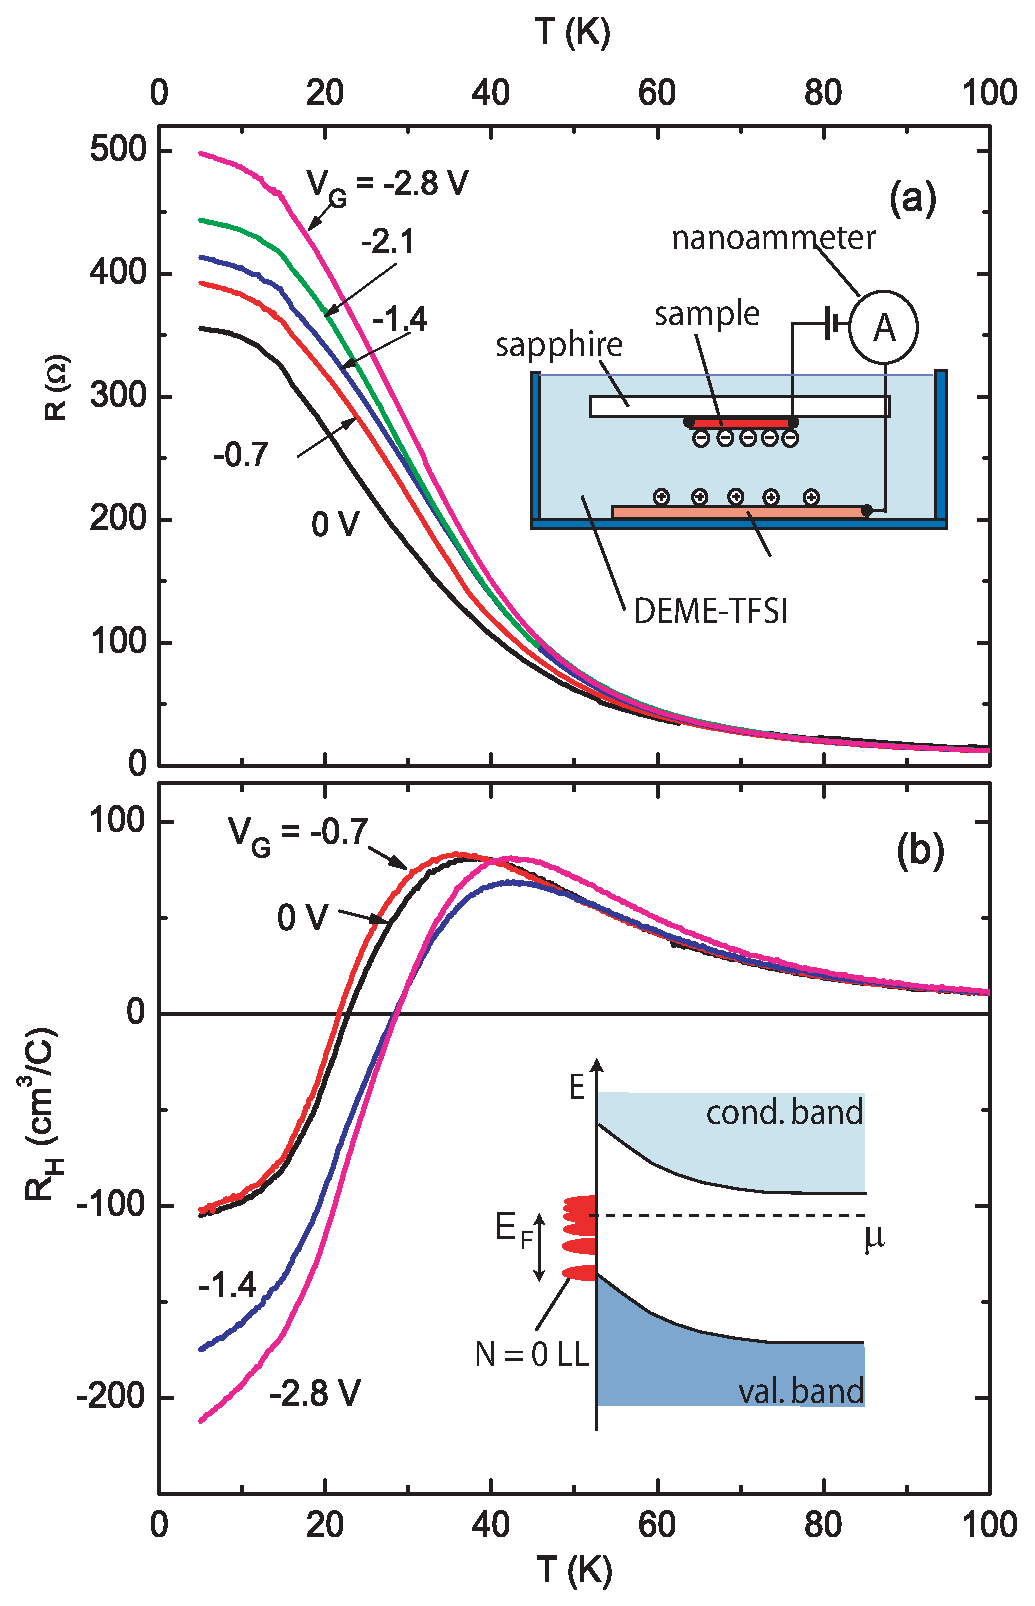
\includegraphics[width=0.75\linewidth]{ch-liquid/figures/FigRR.eps}
\caption{\label{figRRH} The resistance $R$ per square (Panel a) and
Hall coefficient $R_H$ vs. $T$ (Panel b) in Bi$_2$Te$_2$Se at selected $V_G$ in Sample 1. 
$R_H$ is measured at fixed $B$ (3 T) using the reciprocal method in Ref. \cite{Sample1987}. When $V_G$ is changed from 0 to -2.8 V, $R$ increases by 40$\%$ and $|R_H|$ increases by 2$\times$ around 5 K. The inset (Panel a) shows 
the cell housing the sample and the ionic liquid DEME-TFSI. The Au gate electrode (a
circular plate of radius 1.5 mm) is separated by 0.5 mm from the sample.
The inset in (b) is a sketch of the band bending induced by liquid gating. 
Negative ions deposited on the crystal leads to upward band-bending and a decrease of surface chemical potential towards the Dirac point. Landau levels formed by the surface electrons are shown as solid half-ovals.
}
  \end{center}
\end{figure}


Though the ionic liquid appears to have a strong power to change the carrier density in the sample, there is a debate about whether such a change is caused by its large capacitance or by certain chemical reactions. To investigate this issue, we set up some measurement in which $V_G$ is reversed, as we will discuss in the appendix. Briefly speaking, we notice that any changes caused by chemical reactions are inherently nonreversible. It means that if the chemical doping is the main reason for the changes in $\rho$ and $n_H$ at finite $V_G$, then the values of $\rho$ and $n_H$ should not return to their starting values by resetting $V_G$ to 0 V, as the chemical damage to the sample could not be recovered. And we can examine such changes at 4 K as the changes in $\rho$ and $n_H$ are most distinct at 4K. Therefore, by cycling $V_G$ we will be able to tell whether severe chemical doping has happened to the sample or not. If the band bending is the dominant effect in our gating experiment and chemical reaction effects are minimal, there will be no hystereses in $\rho$ and $n_H$ (measured at 4 K) as $V_G$ is cycled. Otherwise, we should be able to notice a large hysteresis. Thus we need to test the absence of resolvable hystereses in $\rho$ and $n_H$ when cycling the gating voltages. In addition, the test can tell us the voltage limit under which the chemical reactions can be neglected. We will show the results of such tests in the appendix. To introduce it briefly, we performed many tests on Sample 3 to investigate details of the ion accumulation in the $V_G$ cycling process over a broad range of gating temperatures (208 $<$ T $<$ 260 K). We have not performed these tests on Samples 1 and 2, from which the detailed SdH results were obtained, as we hope to minimize stress damage to their surfaces.

\begin{figure}[!htbp]
  \begin{center}
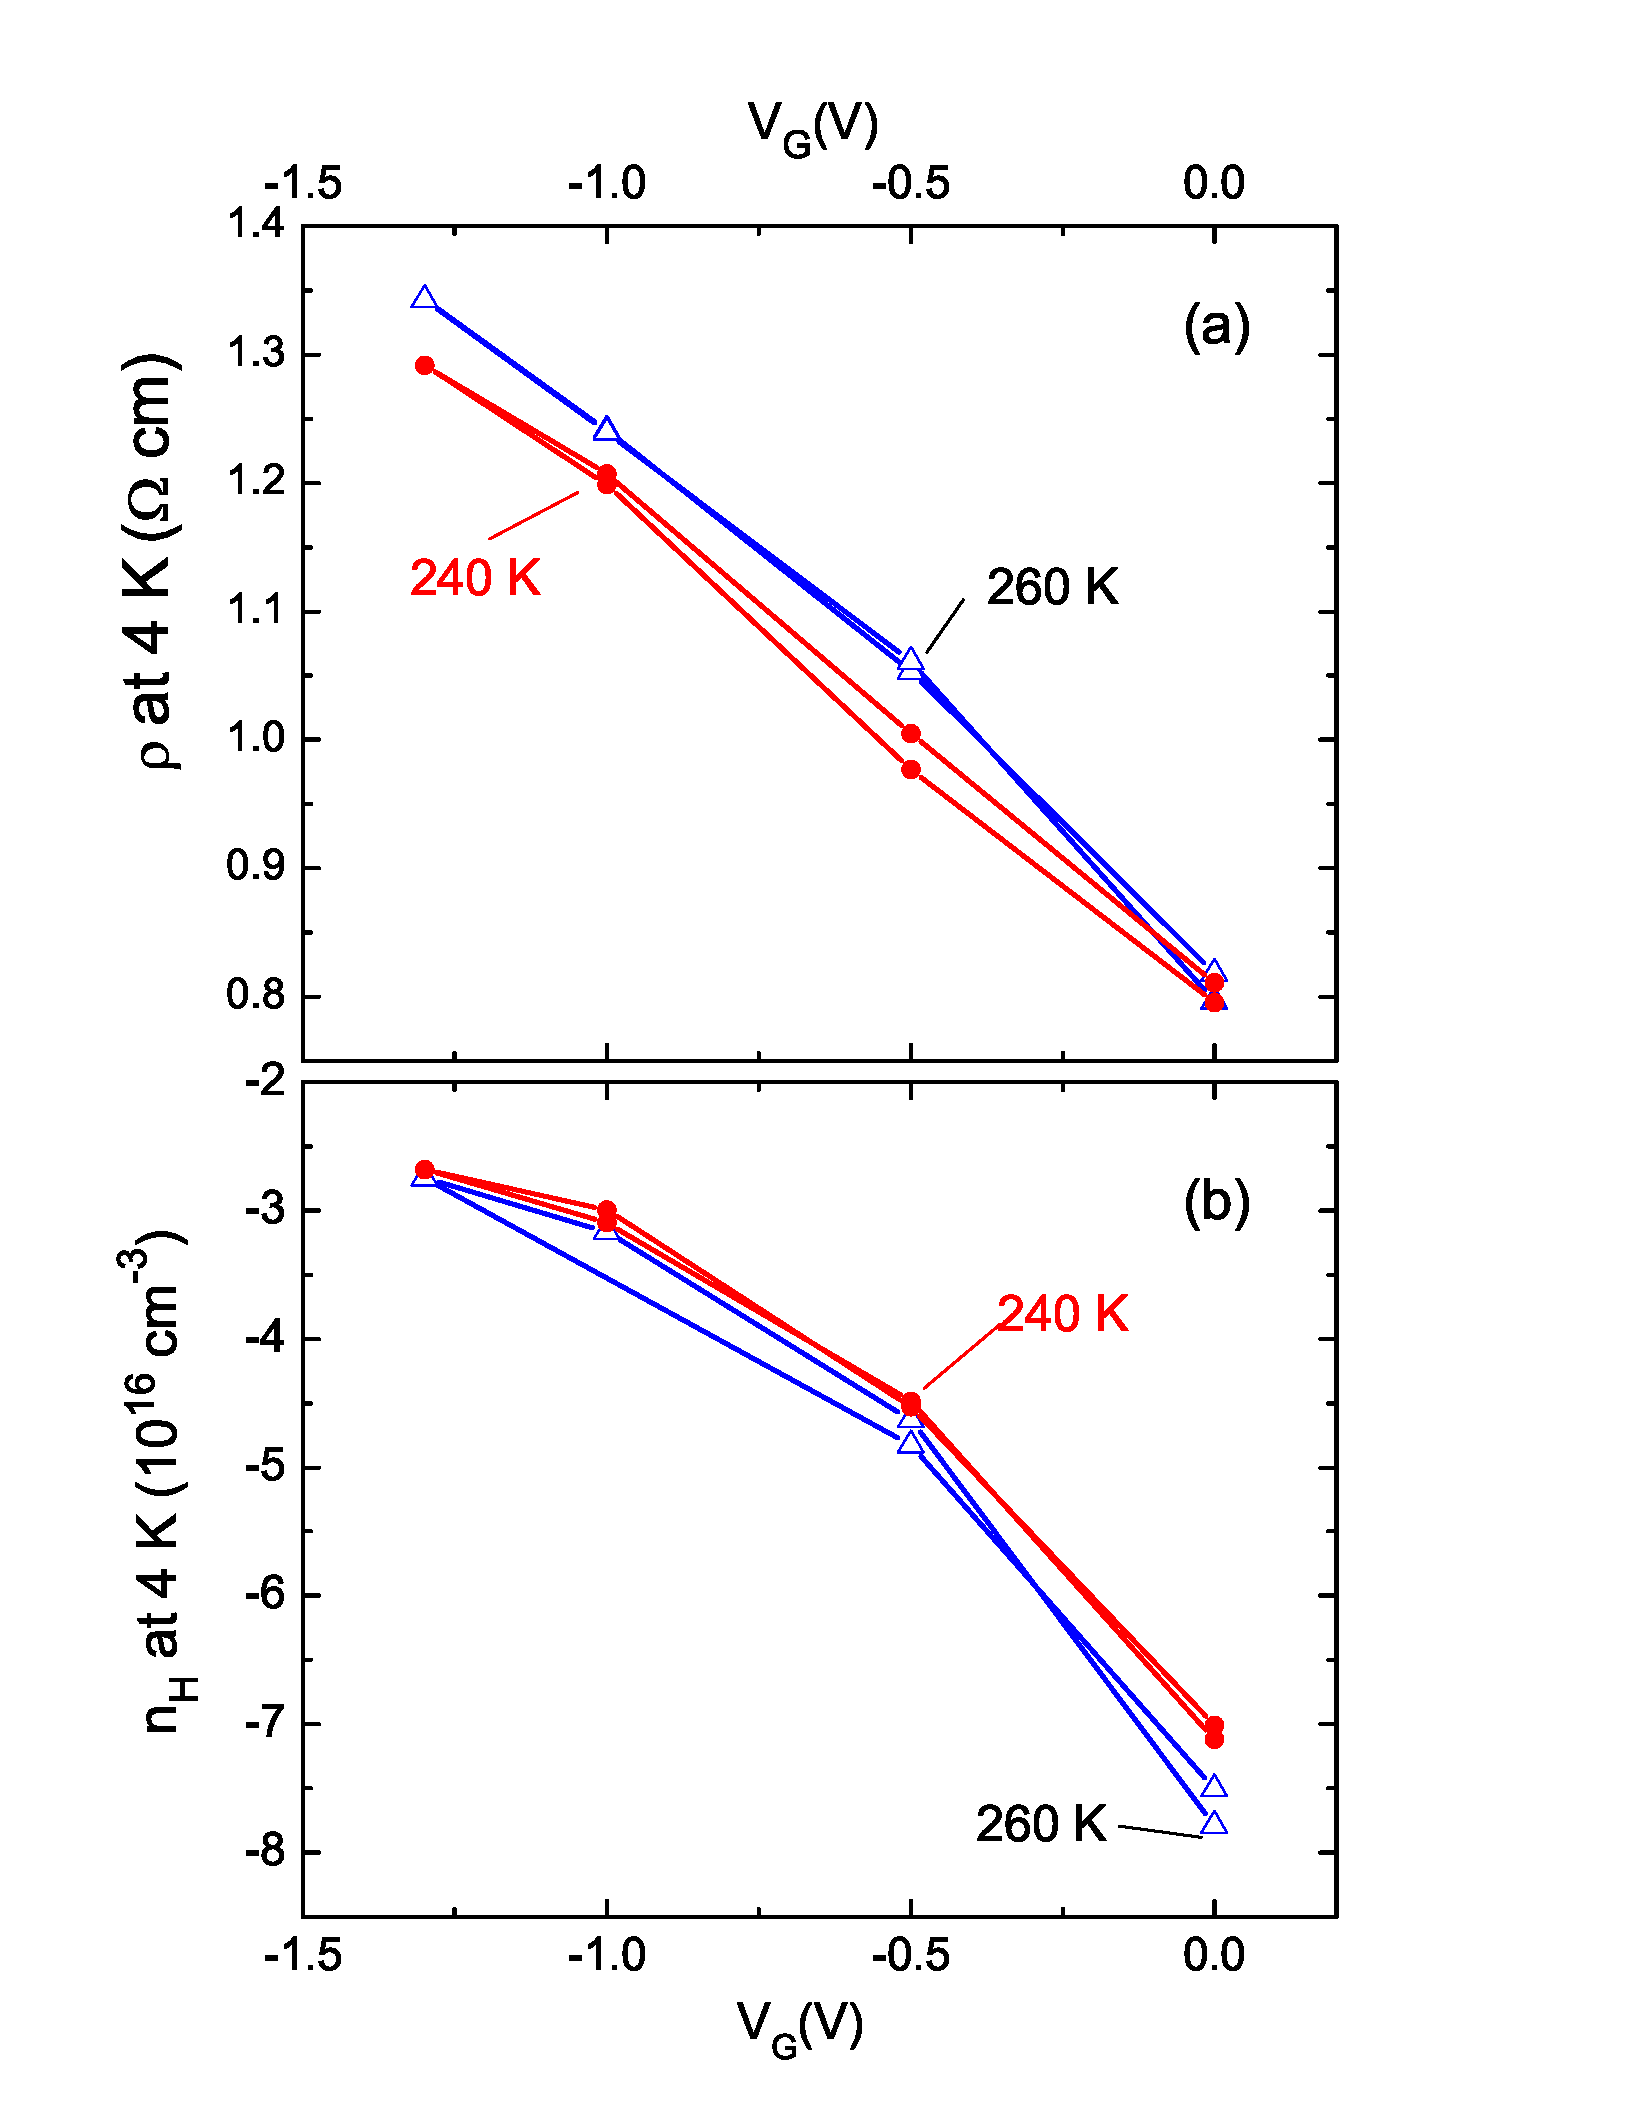
\includegraphics[width=0.75\linewidth]{ch-liquid/figures/FigRvsVG.eps}
\caption{\label{RvsVG} 
Test experiments to show negligible hysteresis in the sample�s resistivity $\rho$ (a) and Hall density $n_H$ (b), as $V_G$ is changed from 0 to -1.3 V, then back to 0 V at temperatures T = 240 and 260 K (Sample 3). The small hysteresis (within the measurement uncertainties) is taken as evidence that the chemical reaction is negligible compared with the physical gating effect. The accumulation time is 800 s in order to collect all the charge.
}
  \end{center}
\end{figure}


Fig. \ref{RvsVG} shows the main result of the $V_G$ cycling experiment on Sample 3. $V_G$ is changed stepwise from 0 to $-$1.3 V and back, while both $\rho$ and $n_H$ at 4 K are monitored at each step. Here $V_G$ is set anew (at the gating T = 240 K and 260 K respectively), and we wait for 800 s to accumulate all the anions before cooling to 4 K for the measurements of $\rho$ and $n_H$. During the change of $V_G$ at 240 K, we also record the transient charging current $I_{trans}$ in order to test whether the accumulated charges are fully reversible and hence cause the band-bending effects. As shown in Fig. \ref{RvsVG}, both at the gating temperature of 240 K and 260 K, $\rho$ and $n_H$ show clear variations at different $V_G$, but they have negligible hysteresis.


Apart from chemical reaction, two other important factors are incomplete melting of the ionic charge configuration when T is too close to the glass transition and the intrinsic (activated) bulk conductance of the ionic liquid. We have investigated these additional factors by measuring the charge accumulation during the $V_G$ change. We discuss them in the appendix. The detailed discussion about the choice of gating temperatures will also be in the appendix.

 
%\begin{figure}[htb]
%  \begin{center}
%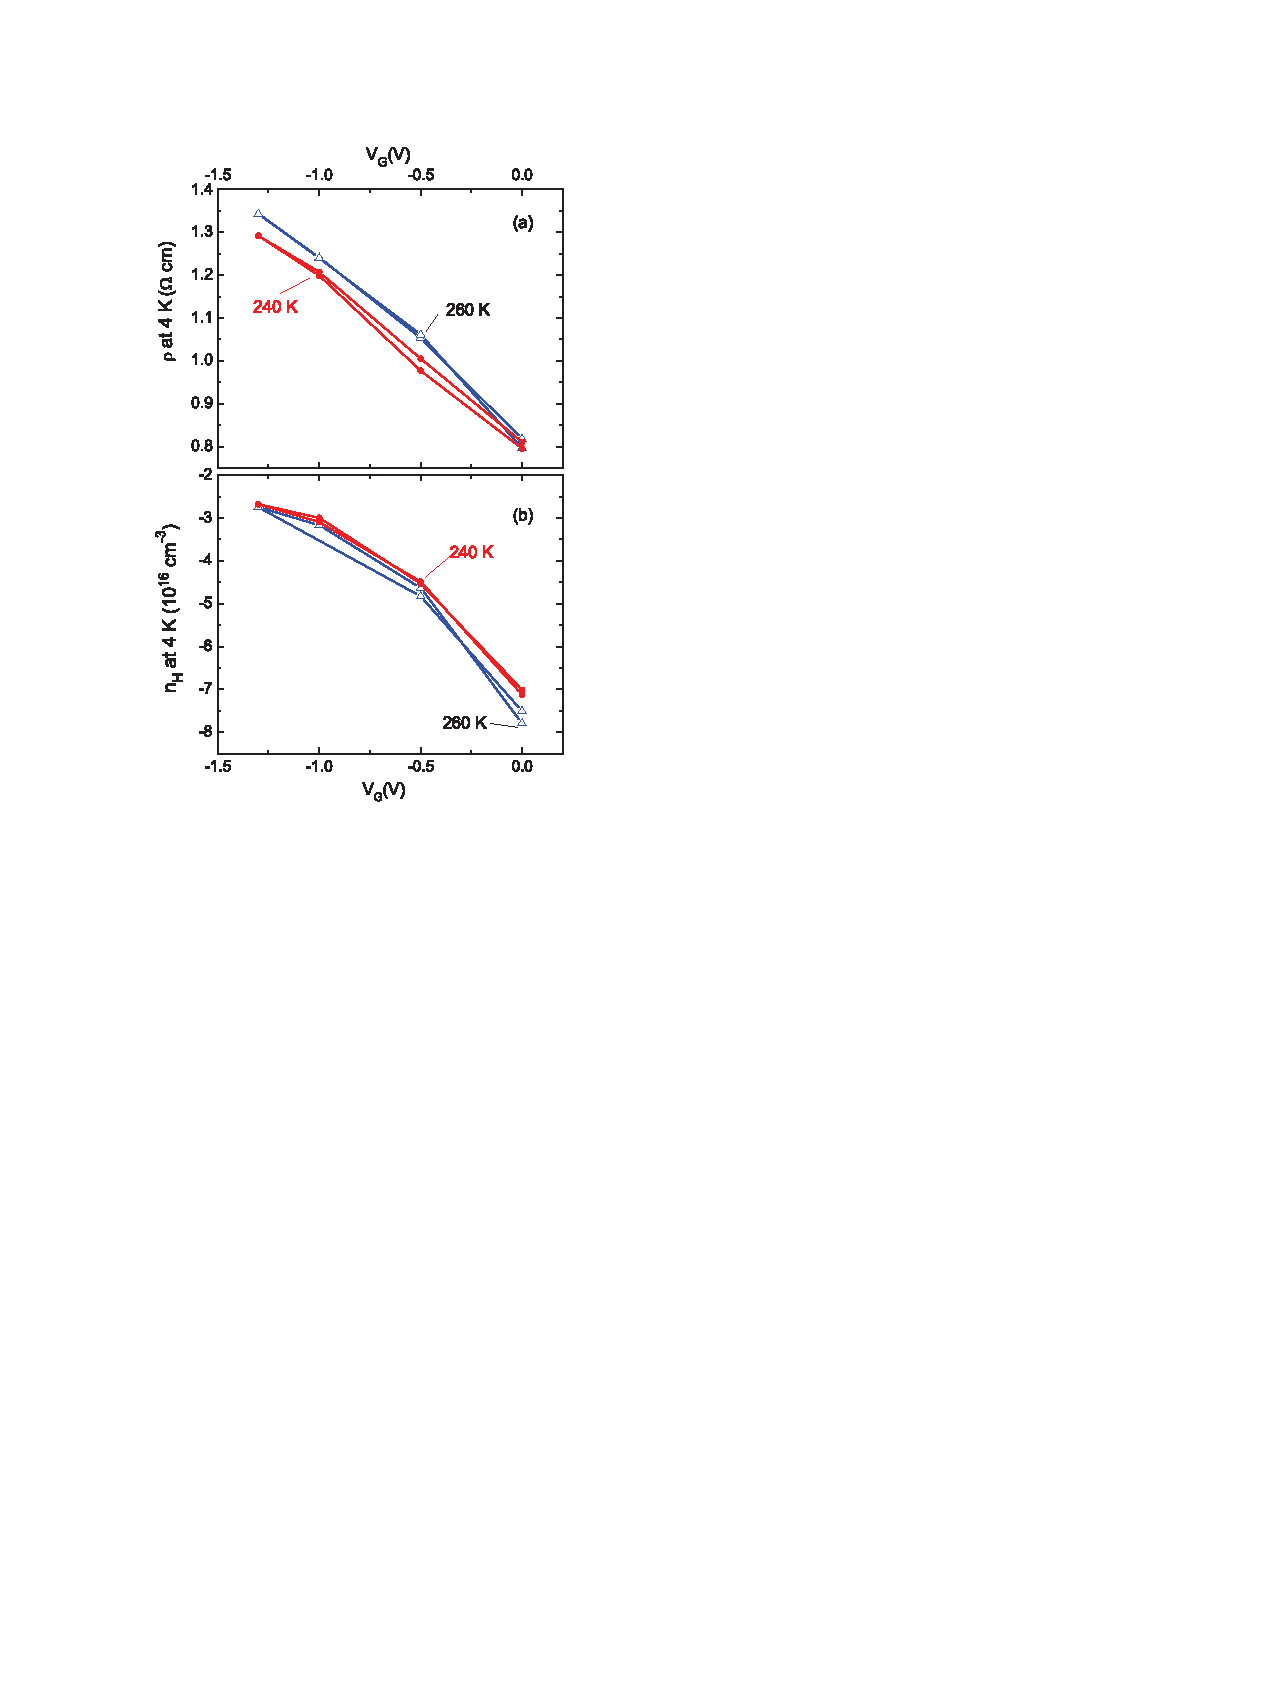
\includegraphics[width=0.9\linewidth]{ch-liquid/figures/nVg.pdf}
%\caption{\label{fignVg} (color online)
%Test experiments
%  \end{center}
%\end{figure} 

%%%%%%%%%%%%%%%%%%%%%%%%%%%%%%%%%%
%%%%%%%%%%%%%%%%%%%%%%%%%%%%%%%%%%
%%%%%%%%%%%%%%%%%%%%%%%%%%%%%%%%%% FIGURE 2


\subsection{Quantum Oscillations in Magnetoresistance under Different $V_G$}

\begin{figure}[!htbp]
  \begin{center}
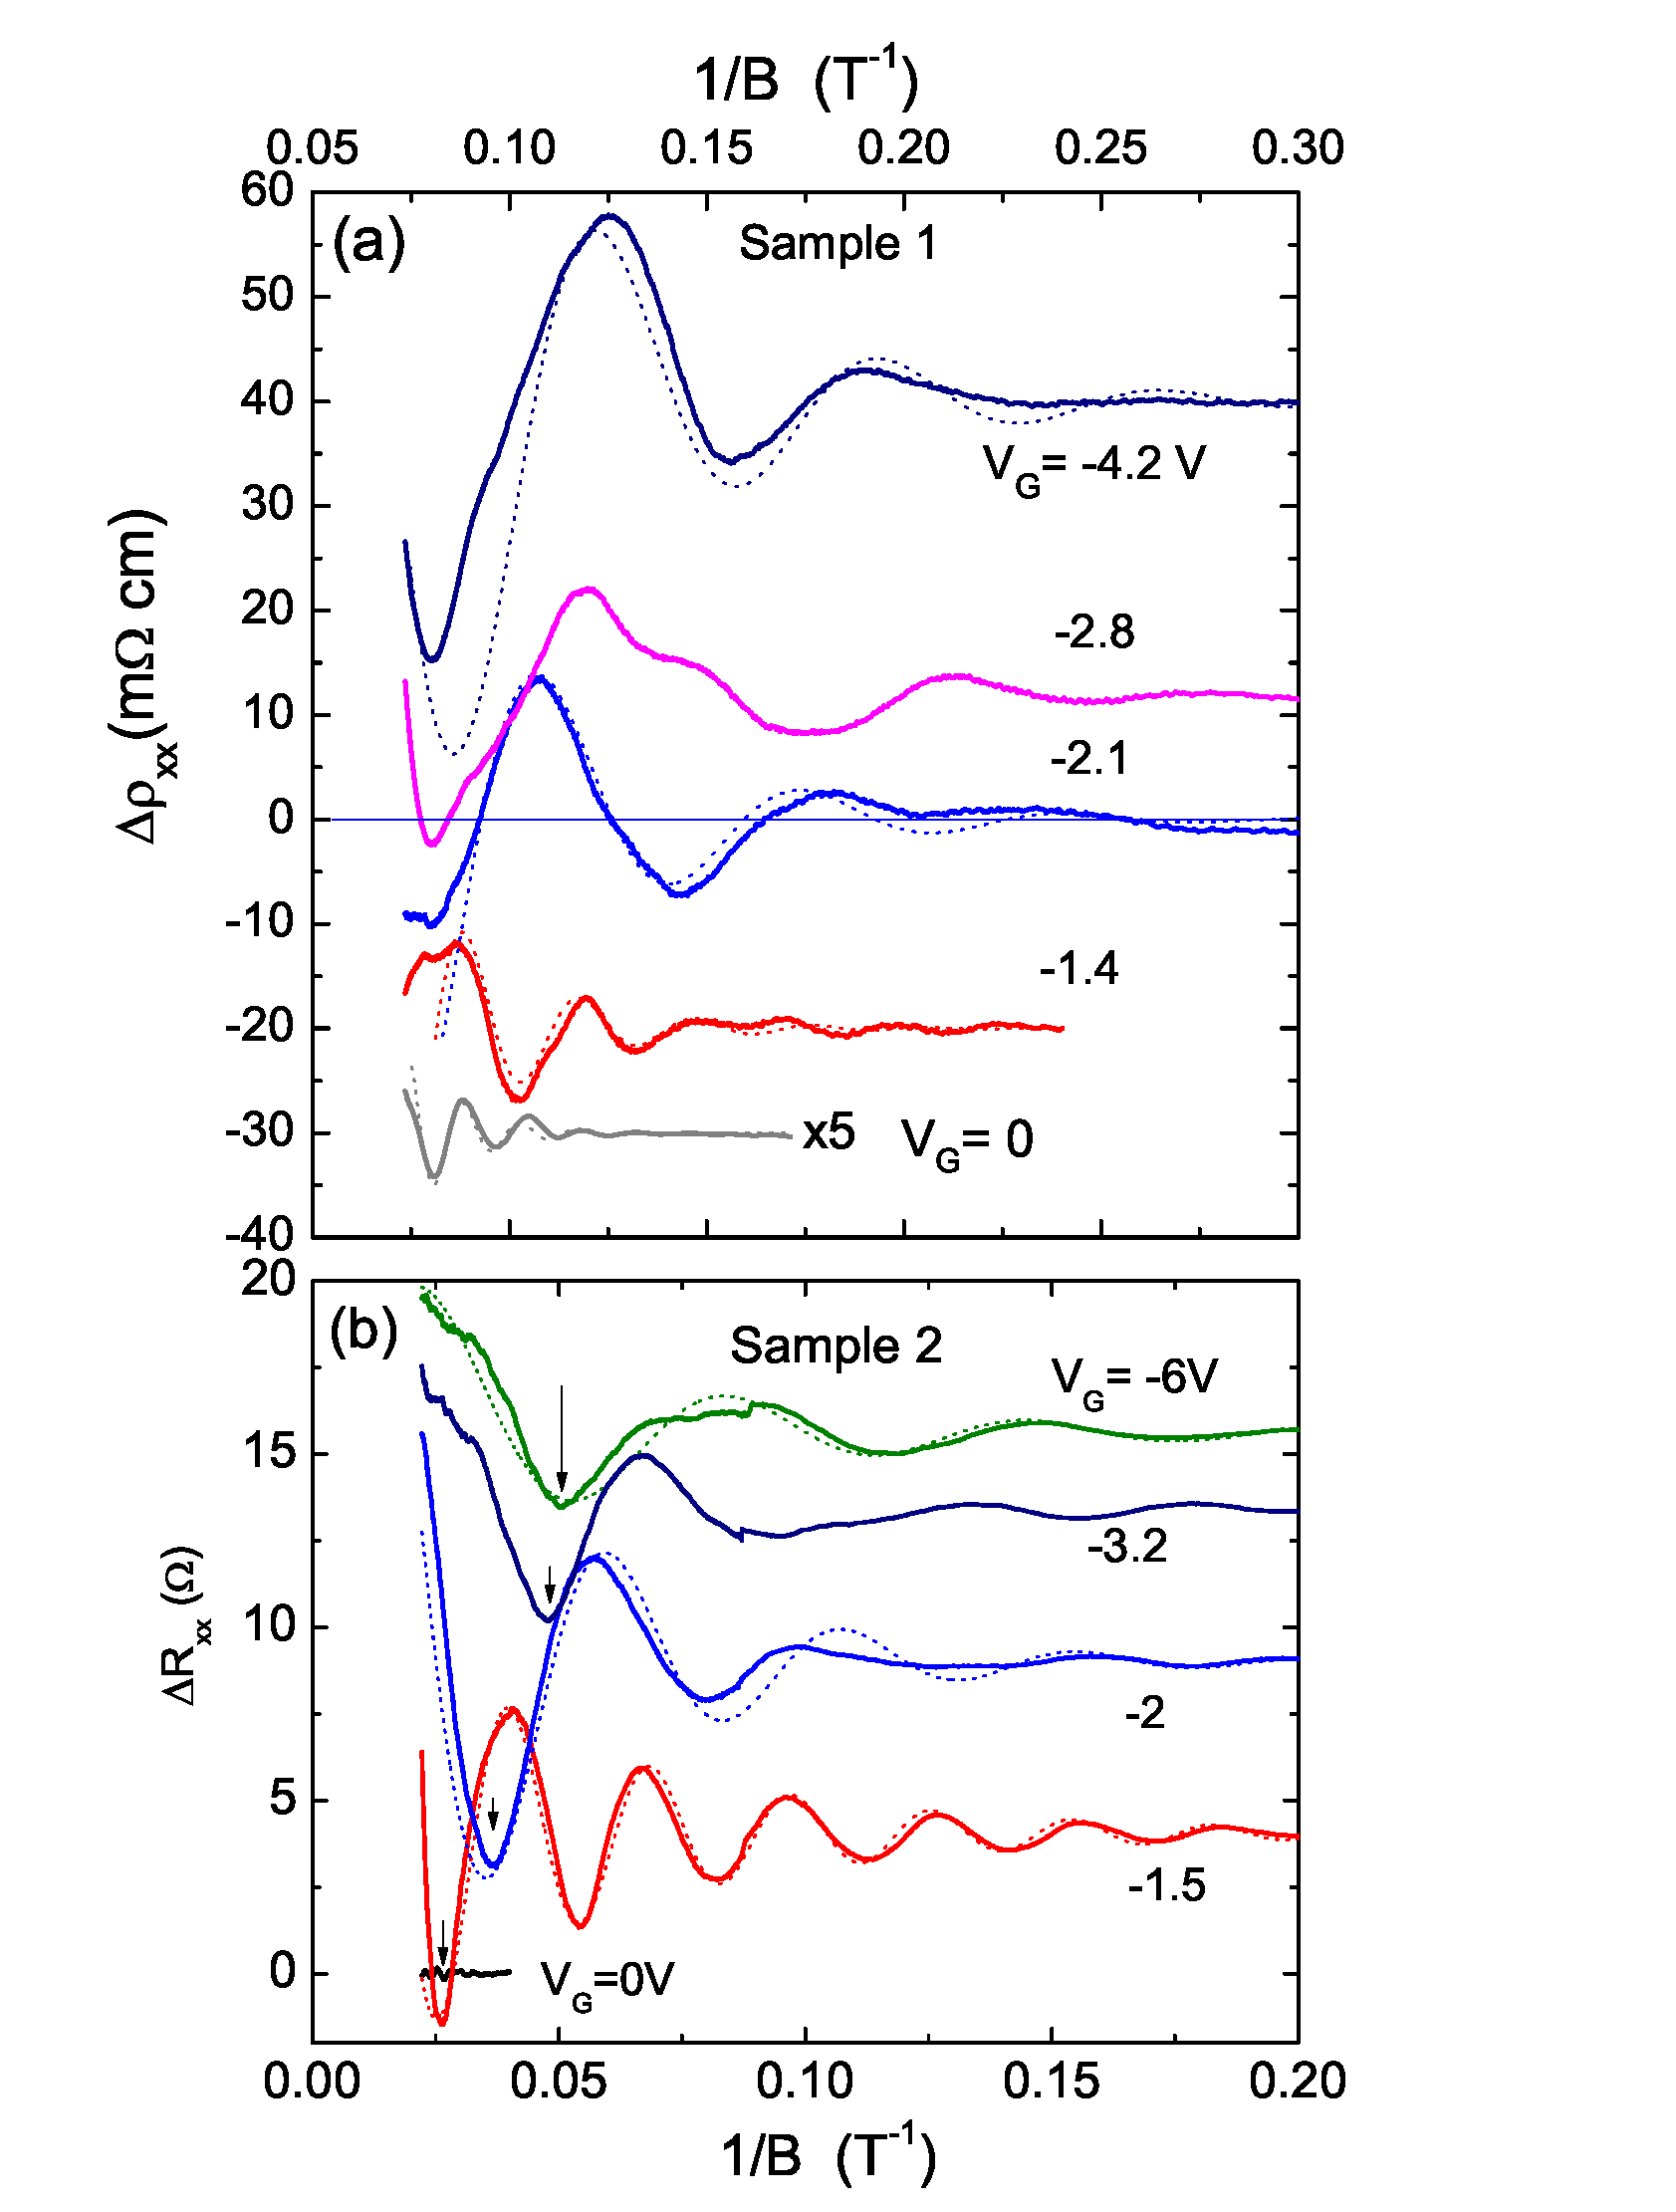
\includegraphics[width=0.85\linewidth]{ch-liquid/figures/FigSdHAll}
\caption{\label{figSdH_Vg}
Traces of SdH oscillations in the resistance versus $1/B$ curves of Sample 1 and 2,
showing systematic changes in the oscillation amplitudes and periods as the gate voltages increase
(bold curves, displaced vertically for clarity). The dashed curves
are fits to the LK expression with one frequency component~\cite{Xiong2012b}. 
Panel (a) shows traces of $\Delta\rho_{xx}$ 
vs. $1/B$ at 5 K measured up to 14 T for 5 values of $V_G$ (Sample 1). 
The largest increase in amplitudes occurs between $V_G$ = 0 V and -1.4 V. The curve
at $V_G = 0 V$ is shown after an amplification of $5\times$. All other curves share 
the same vertical scale. Panel (b) displays traces of $\Delta R_{xx}$ vs. $1/B$ at 0.3 K 
measured up to 45 T at $V_G$ as indicated (Sample 2).
Arrows indicate $n=\frac12$ ($E_F$ at center of broadened $N$ = 1 LL). 
}
  \end{center}
\end{figure} 

At each $V_G$, the magnetoresistance curves for both Sample 1 and 2 display giant SdH oscillations. In Fig. \ref{figSdH_Vg} we have subtracted a smooth background $\rho_B$ from the raw data to emphasize the SdH oscillatory part of the resistance. Therefore, the oscillatory part is $\Delta \rho_{xx} \equiv \rho_{xx} - \rho_{B}$, where $\rho_{B}$ is a smooth background. Fig. \ref{figSdH_Vg}a displays plots of $\Delta\rho_{xx}$ v.s. $1/B$ in Sample 1 for 5 different gate voltages. The period of the SdH oscillations clearly has a large monotonic increase as $V_G$ changes from 0 to -4.2 V, indicating a decreasing $E_F$ of the $n$-type surface states as we expected. Unexpectedly, the SdH amplitudes are strongly enhanced between $V_G = 0$ and -2.1 V (to show the former oscillations in the figure, we have amplified its amplitudes by 5$\times$). The dotted curves are the best fits ~\cite{Xiong2012b} to the Lifshitz-Kosevich (LK) expression for SdH oscillations using only one frequency component. From the fits, we can infer how the surface mobility $\mu_s$ changes with $V_G$ (see below). We find the same trend in Sample 2, which has a higher starting surface density $n_s$ but is taken to $B$ = 45 T (Fig. \ref{figSdH_Vg}b). Although the SdH oscillations are not resolved at $V_G=0$ V, they become prominent starting at $V_G$ = -1.5 V. From the fittings, we also notice that the steepest change in $\mu_s$ of Sample 2 occurs between $V_G$ = 0 and $V_G$ =$-$1.5V, at which $\mu_s$ =2800 $cm^2/(Vs)$. At a larger gating voltage, it saturates ($\mu_s$ = 3000 $cm^2/(Vs)$ at $-$6 V) as the gating effect saturates. 





%%%%%%%%%%%%%%%%%%%%%%%%%%%%%%%%%%
%%%%%%%%%%%%%%%%%%%%%%%%%%%%%%%%%%
%%%%%%%%%%%%%%%%%%%%%%%%%%%%%%%%%% FIGURE 3




%%%%%%%%%%%%%%%%%%%%%%%%%%%%%%%%%%
%%%%%%%%%%%%%%%%%%%%%%%%%%%%%%%%%%
%%%%%%%%%%%%%%%%%%%%%%%%%%%%%%%%%% FIGURE 4




\section{Analysis of the Experimental Results}
\label{sec:liquid:analysis}

\subsection{Analysis of the Quantum Oscillations}
In a strong magnetic field perpendicular to the sample surface, the Dirac surface electrons are quantized into Landau levels (LLs) with quantum numbers $N = 0,1,\cdots$. Here we take the same definition of the index field $B_n$ as in Ref. \cite{Xiong2012b}, which is also the same as our previous chapters. Thus $B_n$ is the field at which $E_F$ falls between two LLs. This definition can also be naturally extended to the quantum Hall regime.
For Schr\"odinger states, the integer $n$ counts the number of 
occupied LLs (the highest filled LL has $N_{max} = n-1$ with the energy $E = (N_{max}+\frac12)\hbar \omega$, where $\omega$ is the cyclotron frequency). Using the level 
degeneracy $Be/h$ per spin, we then have $1/B_n = ne/(hn_s)$ 
($n_s$ is the surface density, $e$ the elemental charge and $h$ is Planck's constant). Thus the Landau index plot in Schr\"odinger case has a zero intercept.

The Dirac electrons have an extra $\frac12$ shift in their LLs as we have
$n+\frac12$ filled LLs when $B = B_n$ (now $N_{max} = n$).
The additional $\frac12$ derives from the $N=0$ LL due to the particle-hole symmetry, or equivalently, 
from the $\pi$-Berry phase intrinsic to each Dirac cone~\cite{Kim}. 
The relation between $1/B_n$ and $n$ is now 
$ 1/B_n = (n+\frac12)(e/h n_s)$ -- a straight line that 
intercepts the $n$-axis at $n = -\frac12$. 
As we discussed in previous chapters, $G_{xx}$ provides a reliable way to decide $B_n$ even when the bulk conductance contributes significantly. And it is a local minimum at $B_n$ for both Dirac and Schr\"odinger electrons. Therefore, we can leverage the difference in the intercepts to distinguish the Dirac electrons and the Schr\"odinger ones.

\begin{figure}[!htbp]
  \begin{center}
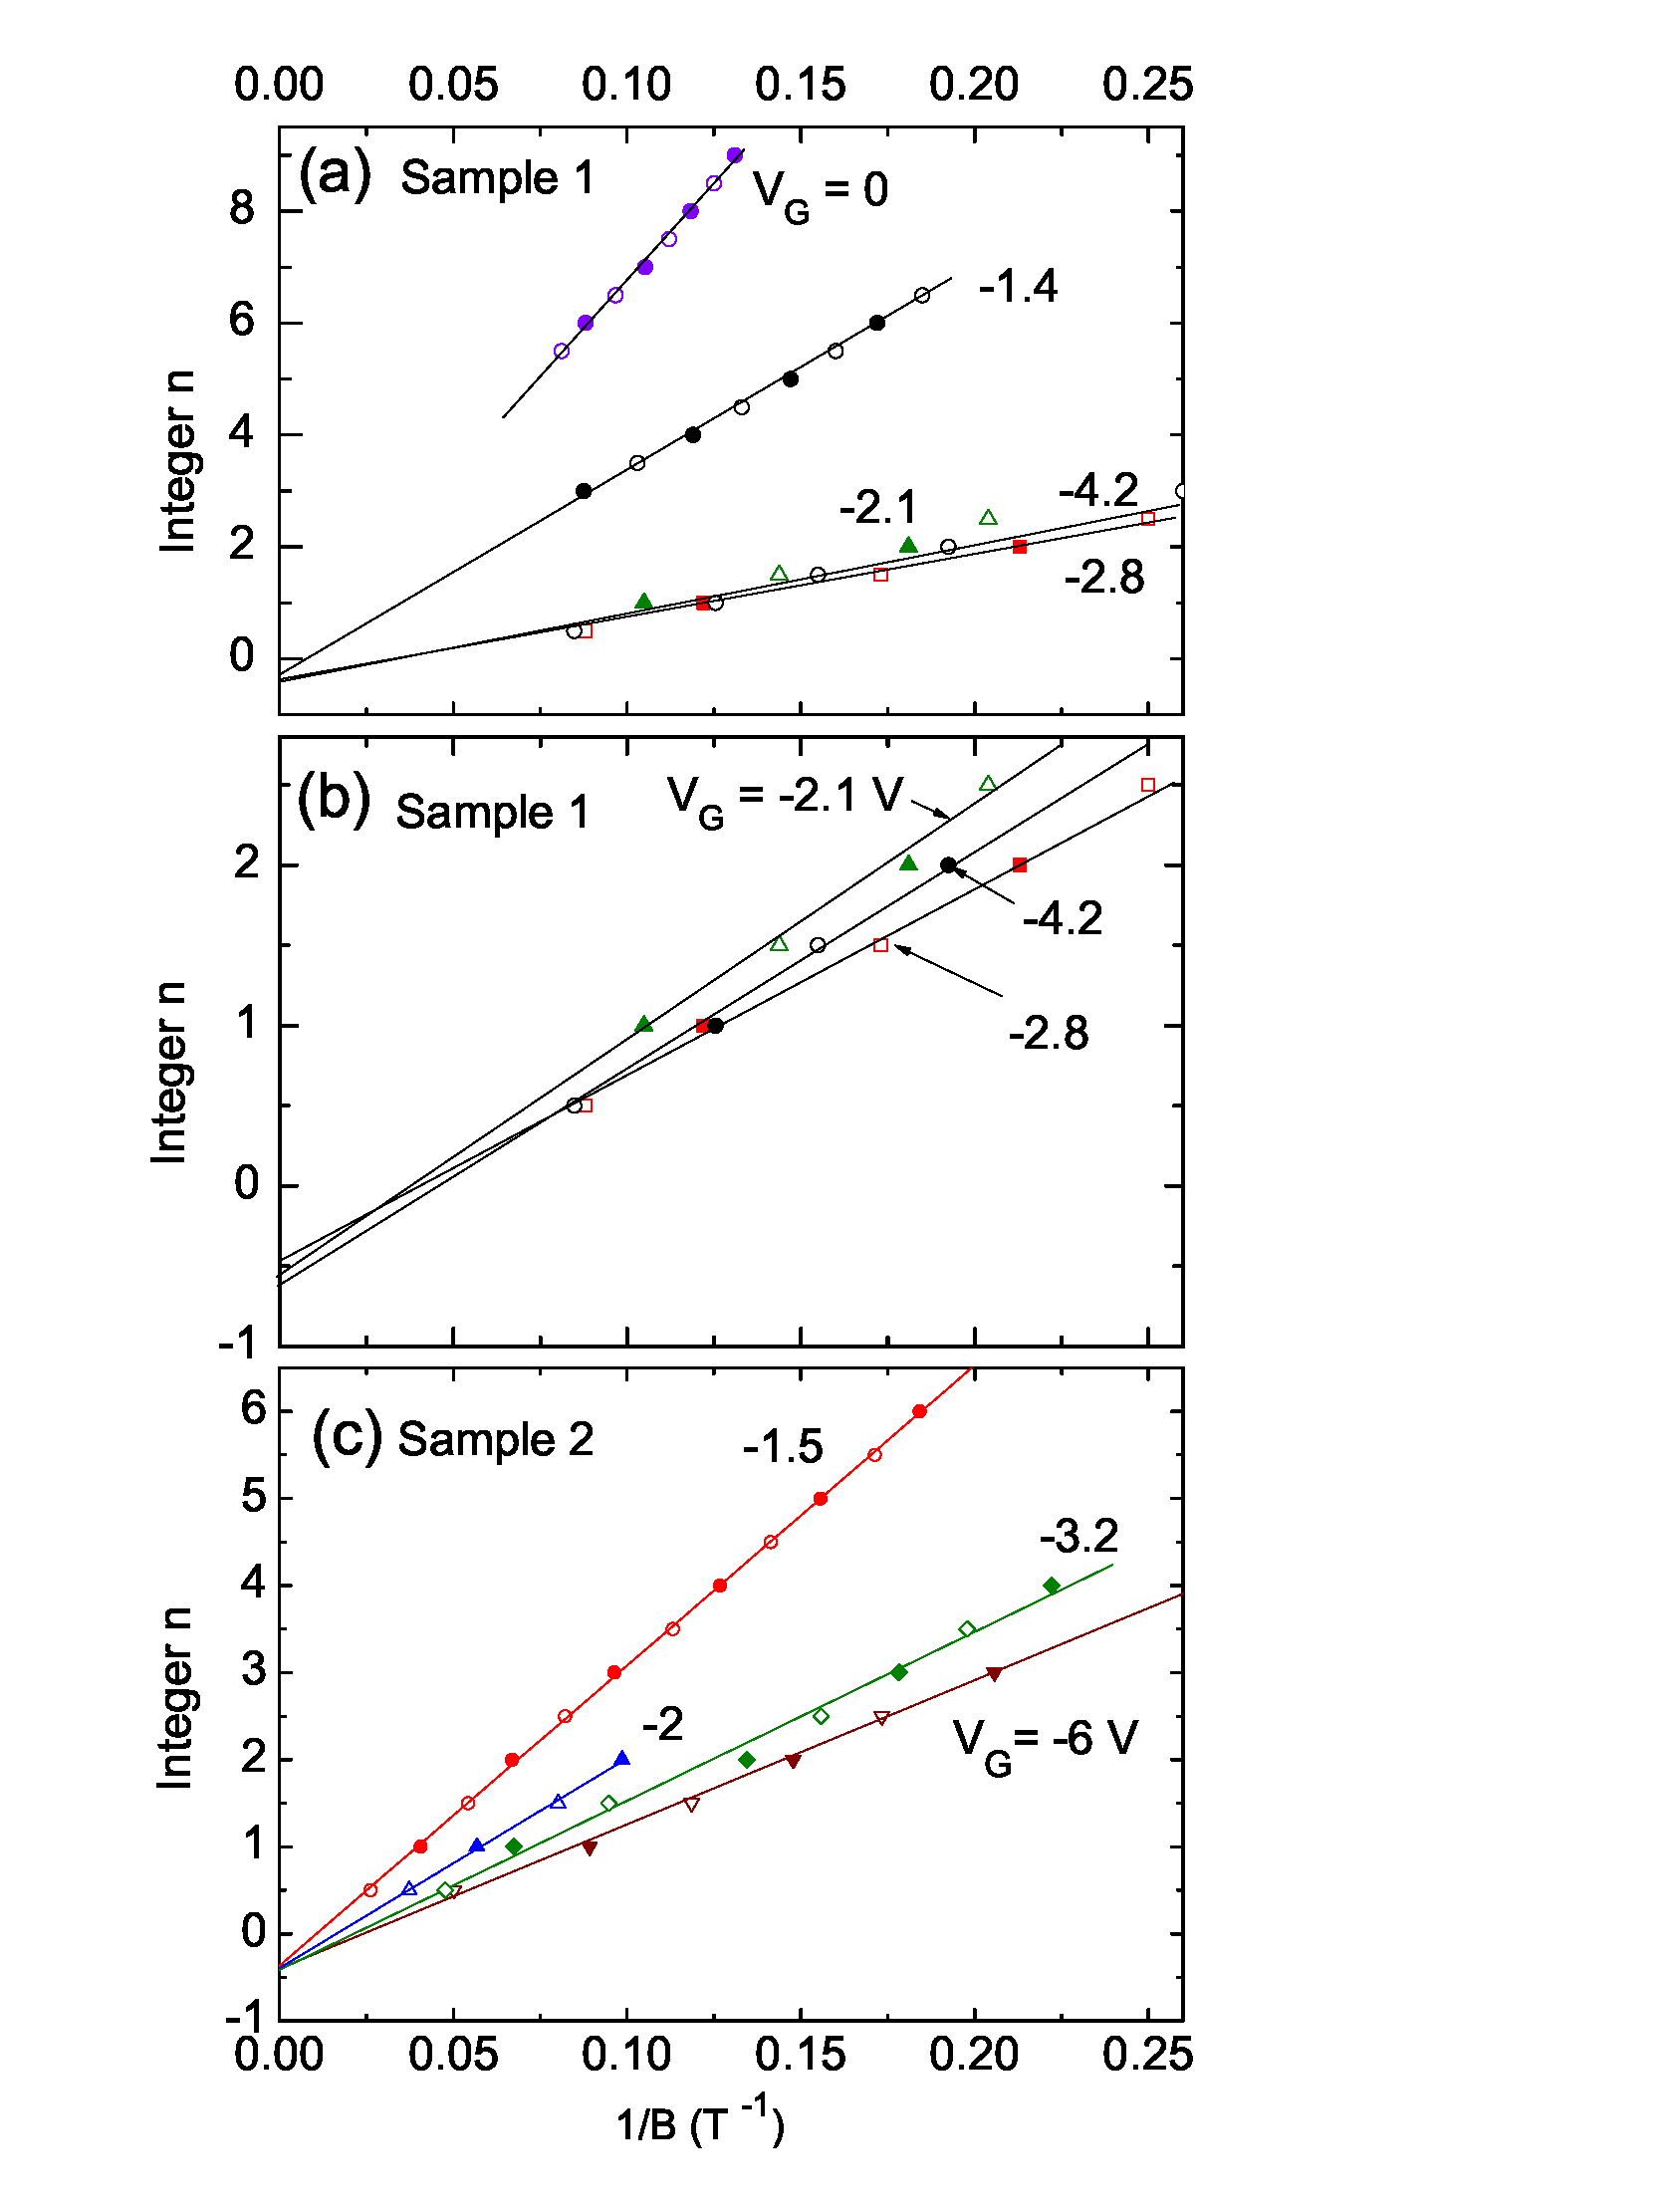
\includegraphics[width=0.85\linewidth]{ch-liquid/figures/FigIndexAll}
\caption{\label{figIndex} 
Index plots of the integer $n$ vs. $1/B_n$ at selected $V_G$ in Sample 1 (Panels a and b) and 2 (Panel c).
Maxima of $\Delta\rho_{xx}$ (solid symbols), corresponding to the index fields $B_n$, are plotted against $n$. Minima (open symbols)
are plotted against $n+\frac12$.
Panel (a): As $V_G$ changes from 0 to -2.1 V, the slope of the best fit lines decreases by six times, indicating a decrease of the carrier density by six times as well. Further increase
in $|V_G|$ leads to saturation of the slope. In Panel (b), the high-bias curves are displayed in expanded vertical scale to determine the intercept. In the limit $1/B\to 0$, the best-fit lines have intercepts at -0.46, -0.56 and -0.61 respectively for different $V_G$. They are close to $\frac12$ (mod 1), consistent with a Dirac dispersion.
The intercepts for Sample 2 (Panel c) also cluster near -0.45 in the limit $1/B\to 0$.
}
  \end{center}
\end{figure} 


However, if the resistivity curves are used to determine the Landau indices, $B_n$ should be identified with the \emph{maxima} in $\Delta\rho_{xx}$ as we discussed in the previous chapter. This is useful when the Hall data are not available. From the $\Delta\rho_{xx}$ v.s. $1/B$ curves in Fig. \ref{figSdH_Vg}, we plot as solid symbols $B_n$ in Sample 1 against the integers $n$ in Fig. \ref{figIndex}a
(the open symbols corresponding to the minima are plotted against $n+\frac12$). The straight lines in the figure are the least square fit to the index plots. The slopes of the fitted straight lines yield the Fermi surface area $S_F$ at different $V_G$. 
As $|V_G|$ increases from 0 to 2.8 V, the slopes of the best-fit lines 
decrease by a factor of 6.4, reflecting a steep decrease in $S_F$. 
This decrease saturates when $|V_G|$ exceeds 2.1 V. Such a decreasing $S_F$ at negative $V_G$ is expected as the anions on the sample surface deplete the $n$-type surface states.  

Then we leverage the intercepts of the fit lines to investigate the Dirac nature of the surface states at different $V_G$. As discussed in previous chapters, sometimes the slope of the index plot changes from the low field regime to the high field part. And the intercepts are fixed by the high field indices. Therefore, we show the high-field behavior for $|V_G|>$ 2.1 V in expanded scale in Panel (b) to obtain a higher accuracy in determining the intercepts. At various large bias values, the intercepts all gather around $n = -\frac12$ 
(-0.46, -0.56 and -0.61) for Sample 1. 

In the Landau index plot for Sample 2 (Panel c), we find that $S_F$ decreases by a factor
of 2 between $V_G$ = -1.4 and -6 V. In the limit $1/B\to 0$, the intercepts are at
$n= -0.35$, -0.40 and -0.42.  These values are all significantly closer to $-\frac12$ than 0 or 1.
The lowest index we obtain at the highest $B$ in both samples is $n_{min}=\frac12$, indicating that $E_F$ lies in the middle of the broadened $N=1$ Dirac LL. As we argued in the previous chapter, such a small $n_{min}$ is important for us to reduce the uncertainties and rigorously exclude an intercept at $n=0$ in the limit $1/B\to 0$. We illustrate the uncertainties incurred in Fig. \ref{figIndexError}a. At $V_G$=0 V, where the LL index is high, the uncertainties $\delta B_n$ in determining the index fields are typically $\pm5\%$ (circles). As shown, it could lead to a considerable spread in the allowed intercepts as we extrapolate the fitted line to the n-axis (the lowest datum corresponds to n = 5.5). By comparison, at the gate voltage $V_G$ = -2.8 V 
(squares), the lowest index is n = 1. This significantly reduces the spread in the allowed intercepts. The same advantage may be achieved by applying an intense $\bf B$ up to 45 T, as done in Ref. \cite{Xiong2012b}.
Therefore, by showing the $-\frac12$ intercepts at different $V_G$, we have provided more conclusive evidence for the Dirac and surface nature of the SdH oscillations on top of our previous discussions.

\begin{figure}[!htbp]
  \begin{center}
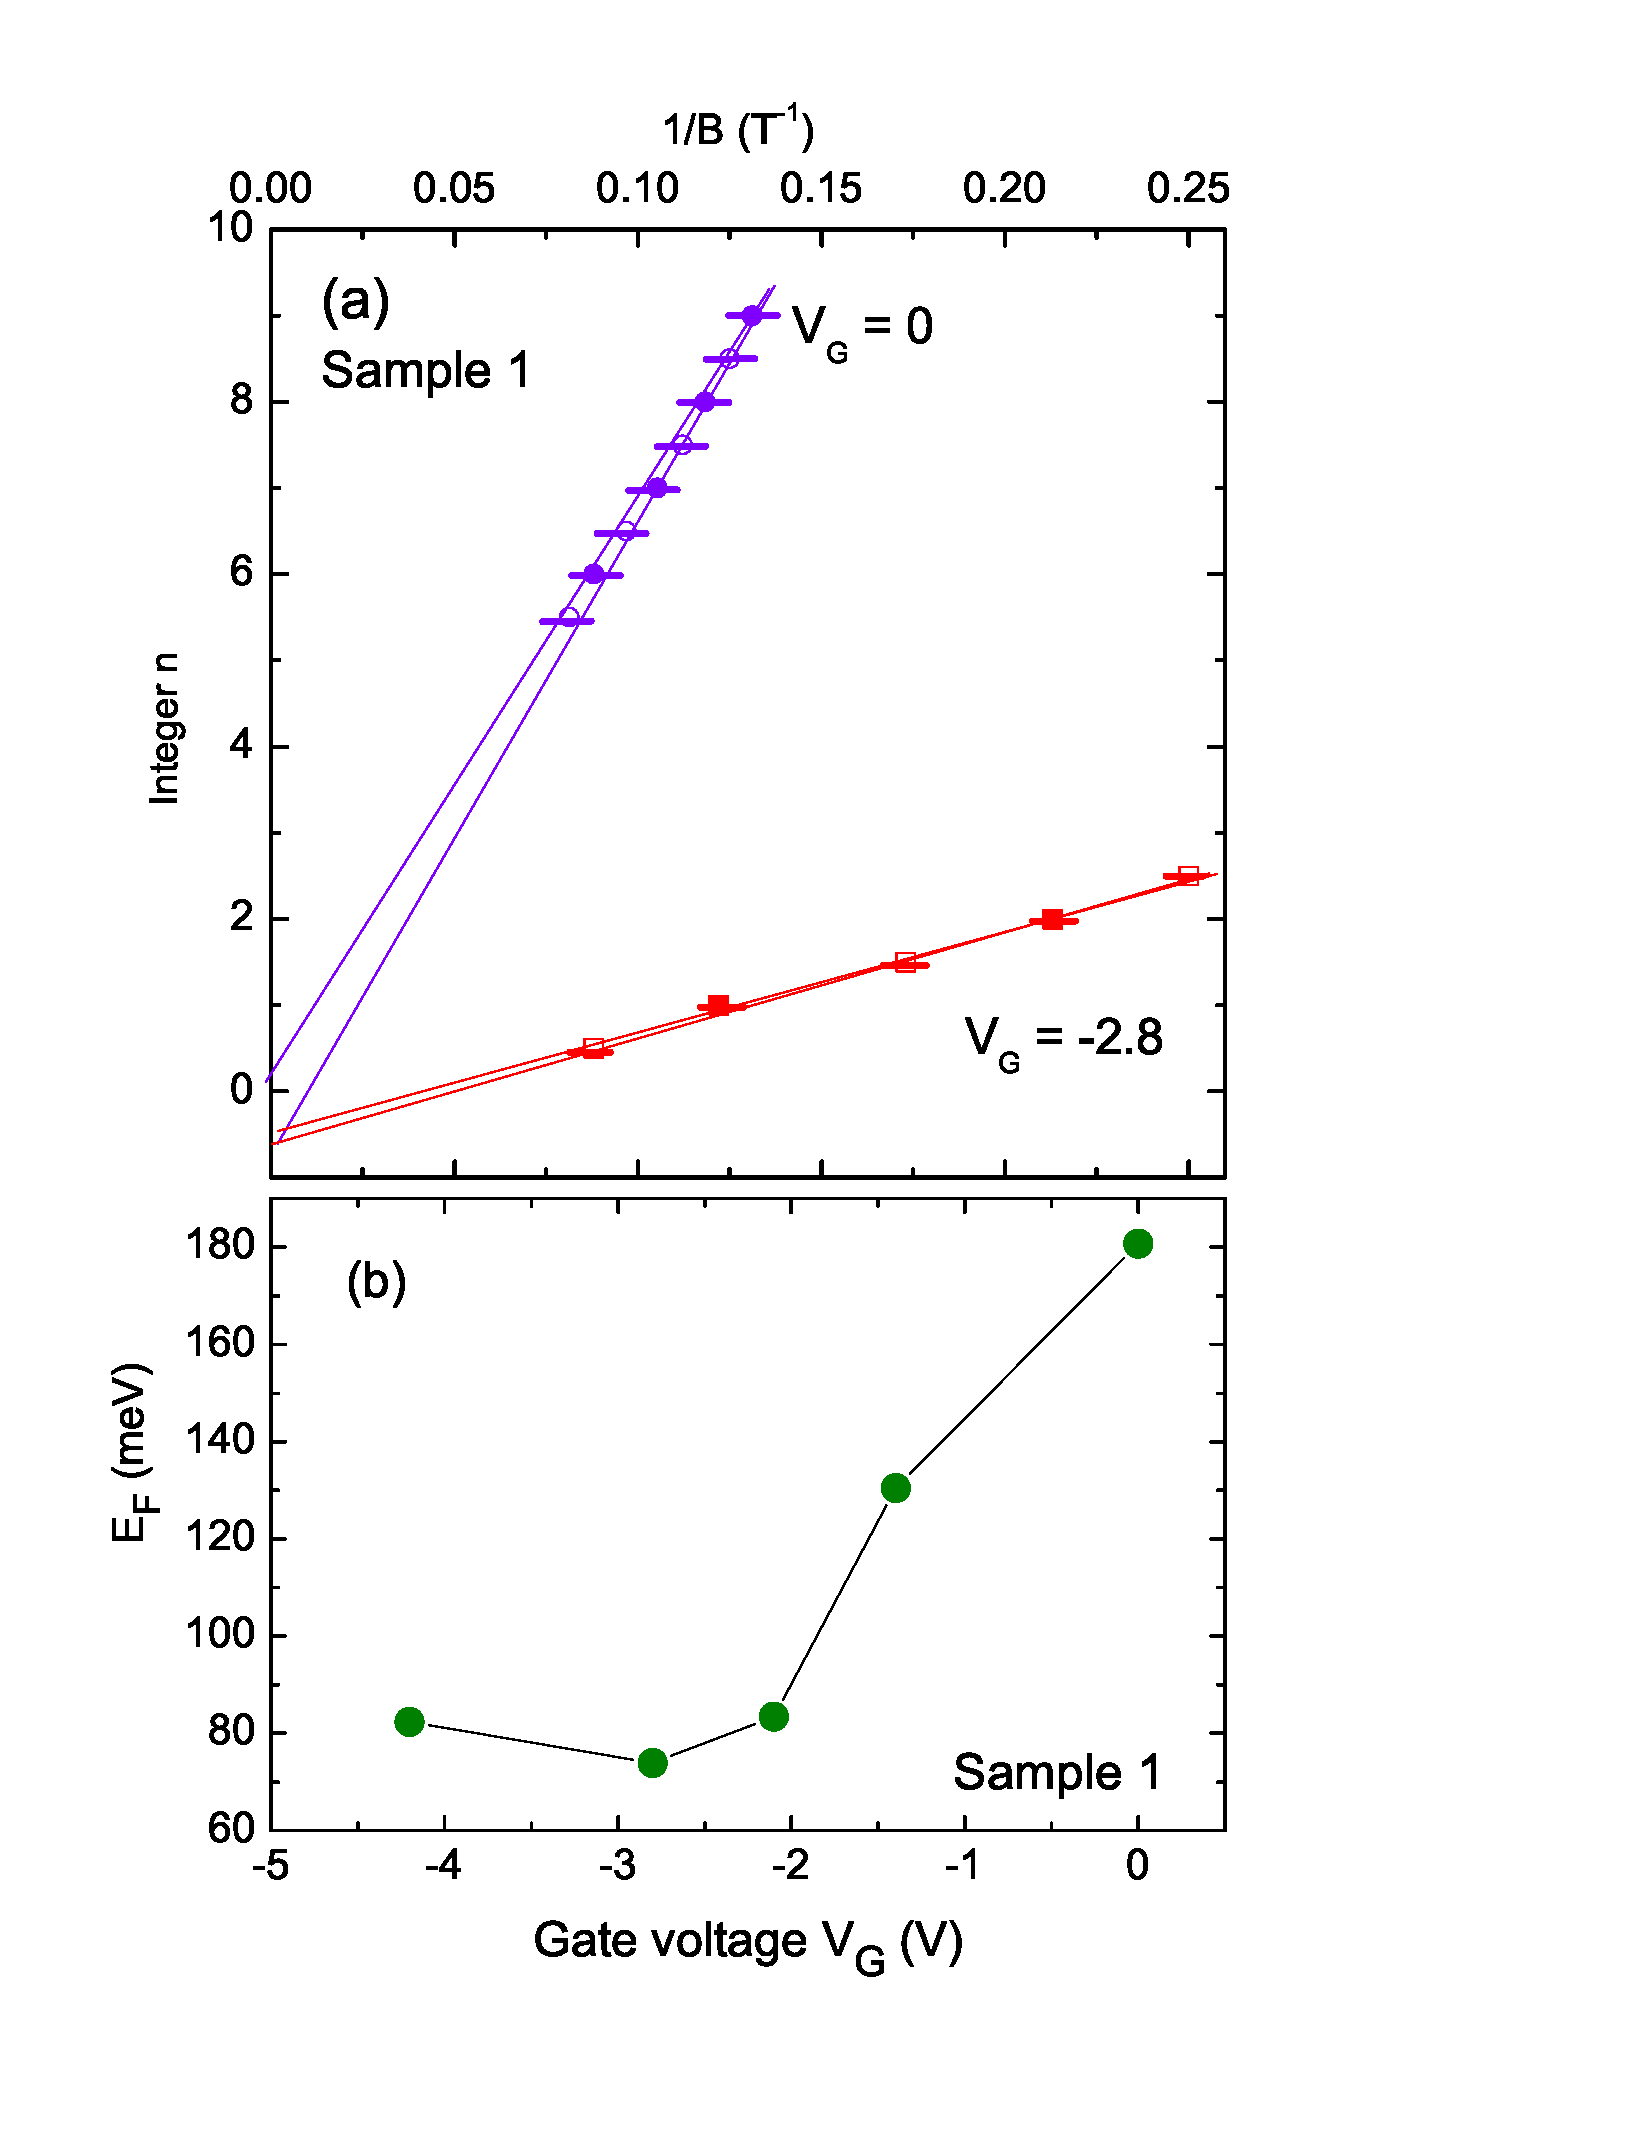
\includegraphics[width=0.85\linewidth]{ch-liquid/figures/FigIndexError.eps}
\caption{\label{figIndexError} 
Comparisons of extrapolations of the index plot to the limit $1/B \to 0$ for index fields measured with $V_G$ = 0 (circles) and measured with $V_G$ = -2.8 V (squares) in sample 1. (b) Variation of $E_F$ with applied $V_G$ in sample 1 ($E_F$ is measured from the Dirac point). The FS cross-section $S_F$ is converted to $E_F$ by $E_F = \hbar v\sqrt{S_F/\pi}$ 
using $v$ = 6$\times 10^5$ m/s~\cite{Xiong2012}. For $|V_G|> 2 V$, the decrease in $E_F$ saturates.
} 
  \end{center}
\end{figure} 


We also calculated the Fermi energy by $E_F=\hbar v \sqrt{S_F/ \pi}$ at different $V_G$, where $S_F$ is inferred from the slopes of the index plots in Figs. \ref{figIndex}. The Fermi velocity we use here is $v_F = 6 * 10^5 m/s$~\cite{Xiong2012}. Fig. \ref{figIndexError}(b) shows that $E_F$ in Sample 1 has been dramatically reduced from 180 meV to around 80 meV when $V_G$ changes from 0 V to -2 V. Thereafter, it remains at $\sim80$ emV at large $|V_G|$. Below we also use this information to estimate the depletion capacitance. Another thing we notice is that $E_F$ stops decreasing when $|V_G|$ exceeds 2 V, possibly due to the saturation of the anion layer and the incoming chemical reactions at large $|V_G|$. It also shows the limitation of the gating power by ionic liquid. Besides, since the Dirac point in Bi$_2$Te$_2$Se is close to the top of the valence band, we have not induced any band inversion in this experiment (otherwise we would have an accumulation layer of holes).

To obtain further information of the surface states at different $V_G$, we fit the SdH oscillations to the Lifshitz-Kosevich expressions (shown as dashed curves) as displayed in Fig. \ref{figSdH_Vg}. The field dependence of the oscillation amplitudes yields the surface mobility $\mu_s$. As shown in Fig. \ref{figHall}b, the surface mobility improves from 720 cm$^2$/(Vs) at 0 V to 2,480 cm$^2$/(Vs) at -4.2 V. Fig. \ref{figHall}c shows that the surface density $n_s = k_F^2/(4\pi)$ (per surface) decreased by approximately 4 times until it saturates at $V_G$ = -2.1 V. We suspect that this saturation at large $|V_G|$ is due to either the chemical reactions or the possibility that $E_F$ starts to touch the top of the valence band.

Another important quantity that characterizes the quality of TI crystals is the conductance ratio between the surface and the bulk $\eta \equiv G^s/G^b$ in zero $B$ (with $G^r \equiv G^r_{xx}(0)$, $r=s,b$). Such ratio describes the portion of the current that flows on the surface of a TI, and can be used to compare different TI materials and devices. It is also of great practical value to improve this $\eta_H$. In our Sample 1, $\eta\sim 0.05$ is quite small (compared with $\eta\sim 1$ obtained in Ref.~\cite{Xiong2012}). However, we notice that the Hall conductance ratio $\eta_H = G^s_{xy}/G^b_{xy}$ which is between the surface and bulk Hall conductance, is enhanced by $\mu_s/\mu_b$ on top of $\eta$ in the Drude model. Since the surface and bulk mobility ratio $\mu_s/\mu_b$ is large in our samples, $\eta_H$ could also be large. 



\subsection{Analysis with a Two-Band Model}

In light of this conjecture, we fit the measured Hall conductivity by a two-band Drude semiclassical model. In the fitting, we fix the surface mobility $\mu_s$ and density $n_s$ with the ones inferred from quantum oscillations. Since the bulk mobility is low, the bulk term only relies on one parameter, i.e.  $n_b\mu_b^2$. Therefore, we only need to tune one parameter to obtain the best-fit curve in the two-band model. This strategy greatly reduces any possibility of overfitting which is typical in a two-band model with multiple parameters. Thus, it can give us reliable results about the bulk properties. The fitting formula we use for $\sigma_{xy}$ is:
\be
\sigma_{xy}= n_se\mu_s\frac{\mu_sB}{t[1+ (\mu_s B)^2]} + n_be\mu_b^2 B,
\label{eq:sxy}
\ee
where the first term is $G^s_{xy}/t$, with $t$ the thickness (50 $\mu$m in Sample 1). 
As $n_s$ and $\mu_s$ are fixed by analysis of the SdH oscillations, the surface term is 
non-adjustable. The second term is the bulk Hall conductivity
$\sigma^b_{xy}$ in the low-mobility limit. We show the fitting results in Fig. \ref{figHall}a and compare it with the field dependence of $\sigma_{xy}$ in the data.
With the sole adjustable parameter $P_b\equiv n_b\mu_b^2$, we find that Eq. \ref{eq:sxy} 
(dashed curves) fits the experimental results very well at multiple $V_G$.
To emphasize the surface contribution, we have also plotted $G^s_{xy}/t$ as inner and faint solid curves in Fig. \ref{figHall}a. 
Combining $P_b$ with the zero-$B$ value of
$\sigma^b_{xx}$, we finally separate and obtain $n_b$ and $\mu_b$ for each value of $V_G$.
We report their values at different $V_G$ in Figs. \ref{figHall}b and \ref{figHall}c. 
The small values of $\mu_b$ (20-30 cm$^2$/Vs) result in a 
large $\mu_s/\mu_b\sim$ 100 and $\eta_H\sim$ 5. We notice that the large $\mu_s$ could also explain the weak-field curvature of $\sigma_{xy}$ in Fig. \ref{figHall}a as the large $\mu_s$ yields a resonance peak at low fields. Also, since the resonance peak generated by $\mu_s$ grows as $\mu_s$ becomes larger, it may also account for the curvature enhancement in $\sigma_{xy}$ with an increasing $|V_G|$.

\begin{figure}[!htbp]
  \begin{center}
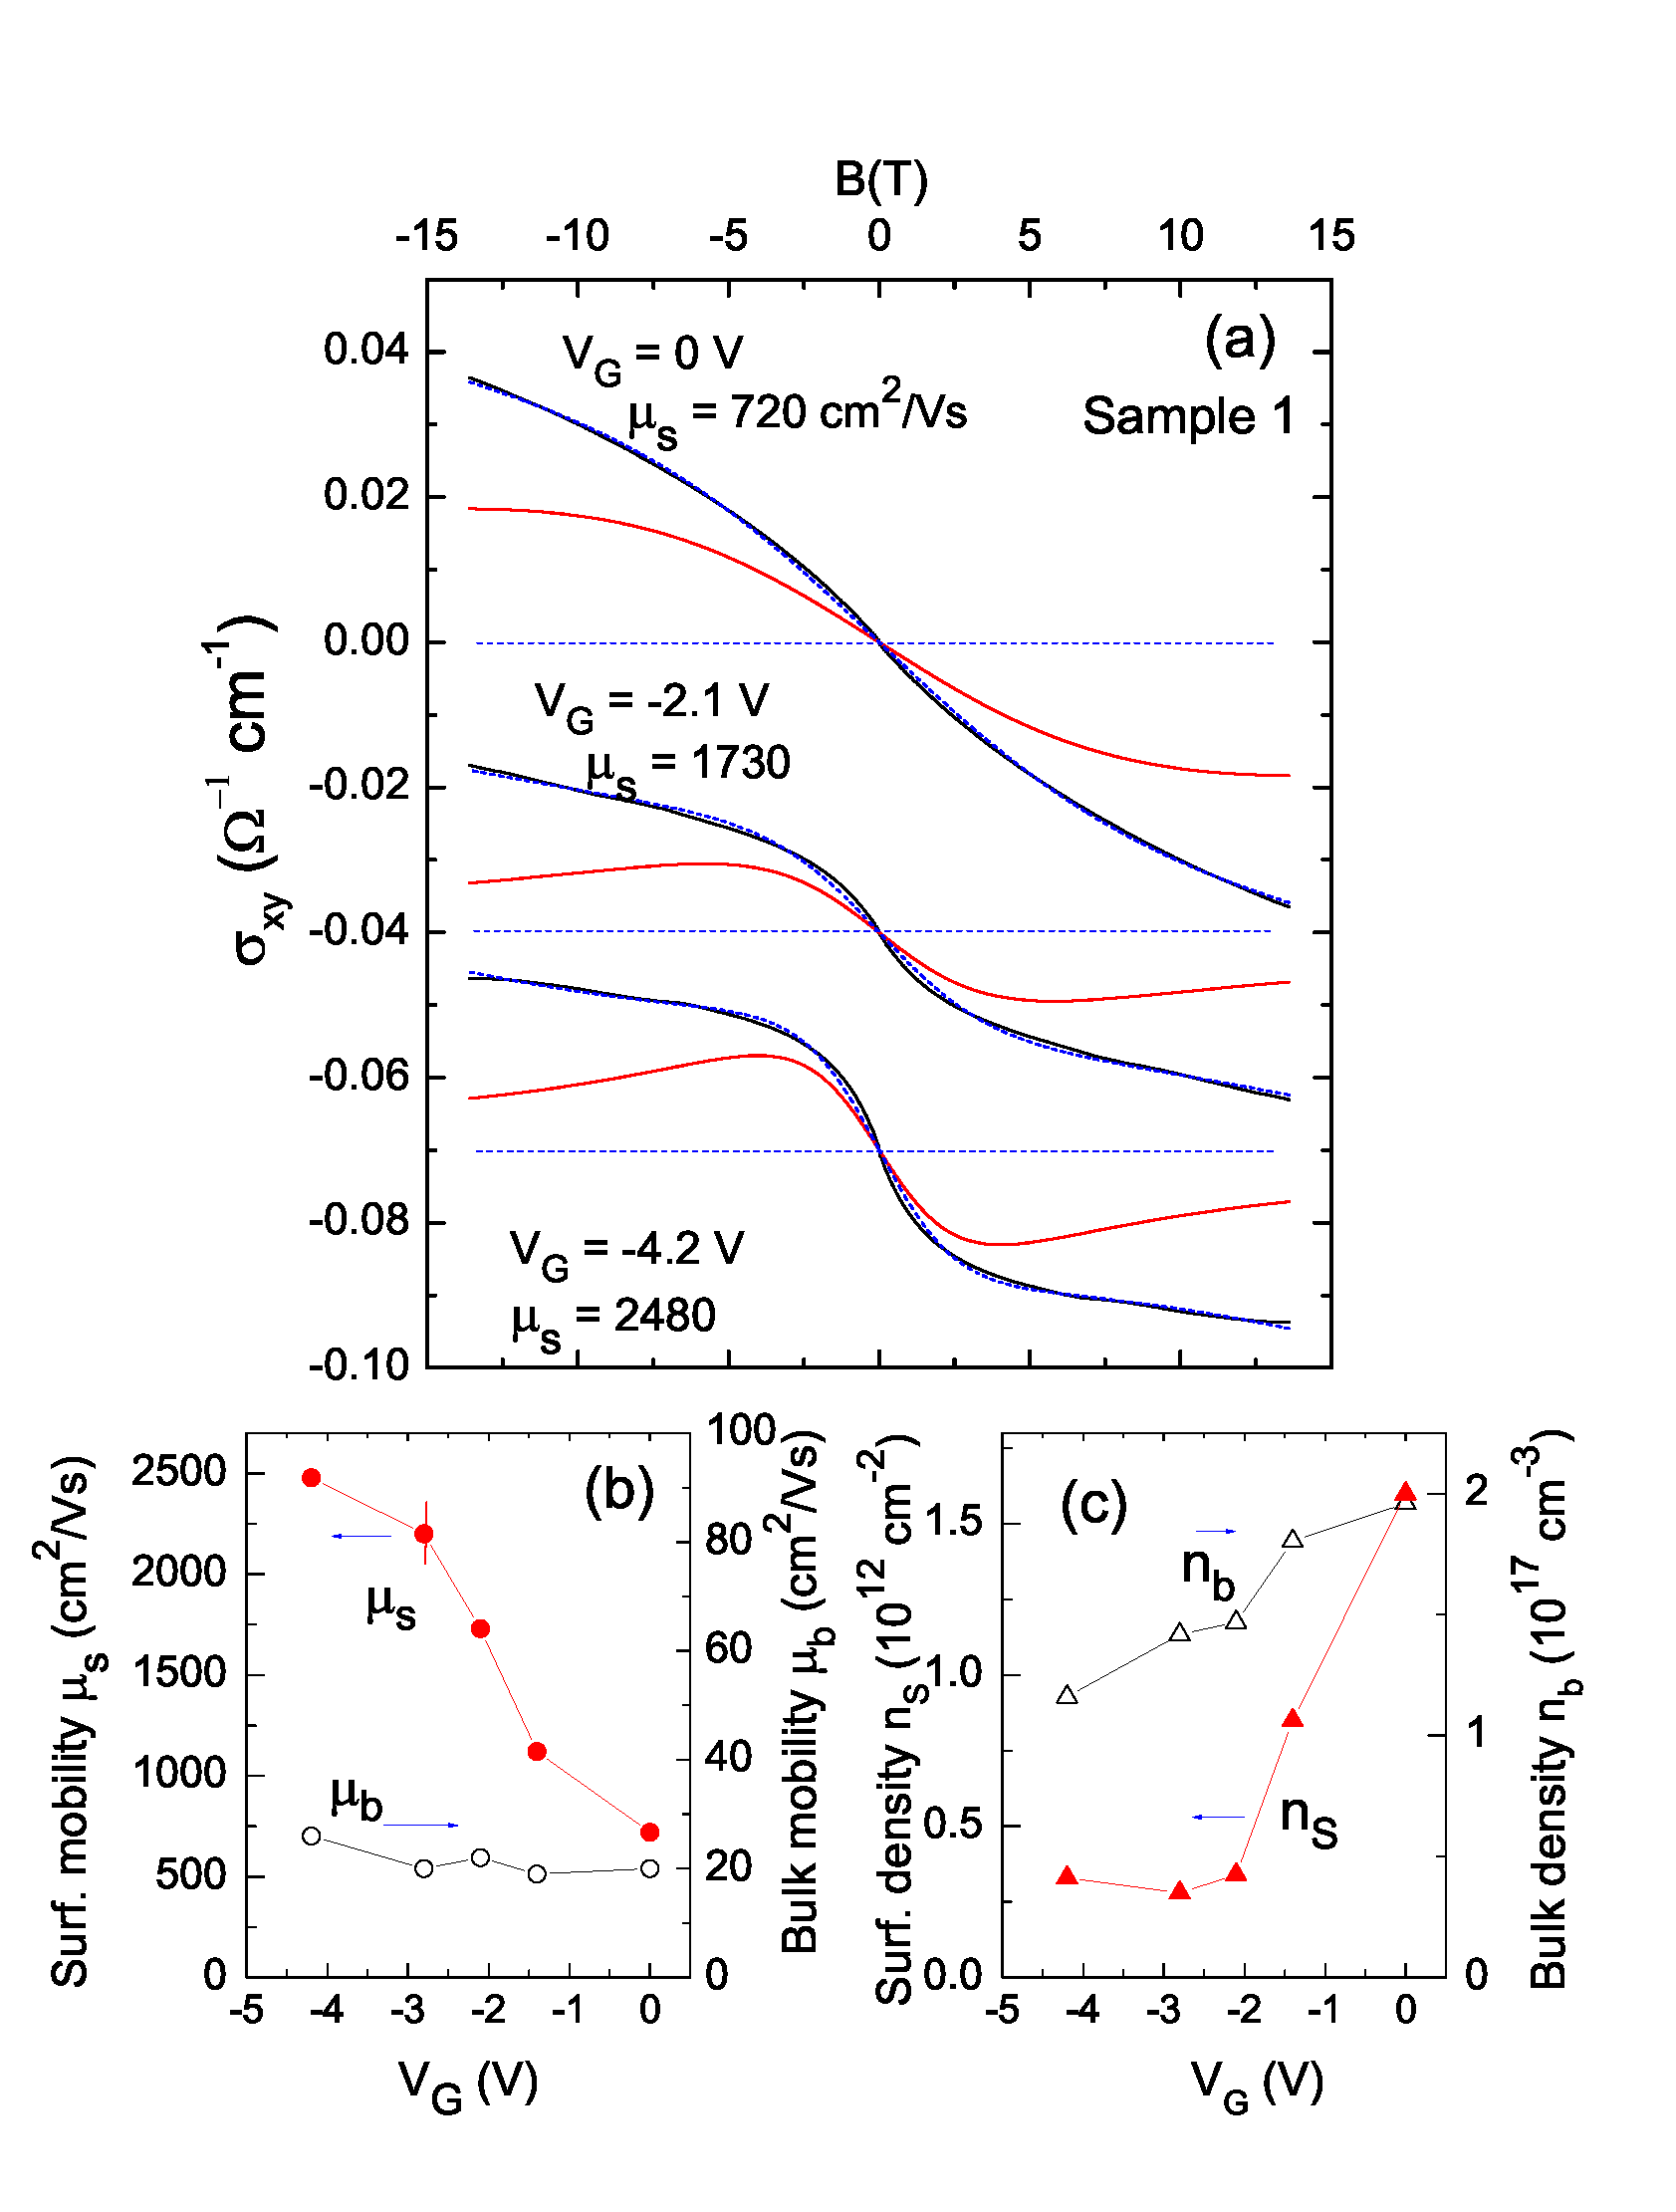
\includegraphics[width=0.85\linewidth]{ch-liquid/figures/FigHallMob3}
\caption{\label{figHall} (color online) 
Panel (a): The observed Hall conductivity $\sigma_{xy}$ vs. $B$ in Sample 1,
showing weak-$B$ curvatures at 3 values of $V_G$
(curves displaced for clarity). At each $V_G$, the outer curves are the 
data (solid black curve) and the fit to Eq. \ref{eq:sxy} (superposed blue dashed curve). The inner
(red, solid) curve is the surface term
$G^s_{xy}/t$ fixed by $n_s$ and $\mu_s$. (Weak SdH oscillations are apparent in the
observed $\sigma_{xy}$.) The difference 
between the outer and inner curves is the bulk term $\sigma^b_{xy}$. 
At $V_G$ = -4.2 V, $G^s_{xy}/t$ accounts for 83$\%$ of
$\sigma_{xy}$ in weak $B$. 
Panel (b) shows that, with increased gating, $\mu_s$ increases from 720 to 2,480 cm$^2$/Vs 
while $\mu_b$ stays very small (20-30 cm$^2$/Vs). Panel (c) 
compares the sharp decrease in $n_s$ with the mild change in $n_b$ with gating. When $|V_G|$ is larger than
2 V, $n_s$ saturates.
}
  \end{center}
\end{figure} 


The above analysis indicates the coexistence of high-mobility surface Dirac electrons and a larger population of bulk electrons in our Bi$_2$Te$_2$Se samples. Because of the 100-fold difference in mobilities,
the Dirac surface electrons account for 83$\%$ of the total weak-$B$ Hall conductance at large $|V_G|$. Since we only includes one surface in calculating the surface Hall conductance, and it already accounts for the majority of the total $\sigma_{xy}$. There is no room left for a comparably large $G^s_{xy}$ for the other surface. With the parameters above, we estimate that the Hall contribution from the other surface 
is less than 2$\%$ of $\sigma_{xy}$. It also implies a low mobility on the other surface ($\mu_s$ is $<$300 cm$^2$/Vs), which explains why we do not resolve the other surface in SdH oscillations.





%The large enhancement of $\mu_s$ (Fig. \ref{figHall}b)
%by the liquid gating method is perhaps the most intriguing 
%feature reported here. To our knowledge, this is the first realization of 
%enhancement of surface SdH amplitudes by an \emph{in situ} technique.%~\cite{mobility}
%A recent STM experiment~\cite{Beidenkopf2011} reveals that
%the Dirac Point closely follows spatial fluctuations of the local
%potential on length scales of 30-50 nm. This could lead to strong scattering
%of surface electrons. We speculate that, under liquid gating, the anions accumulate
%at local maxima in the potential, thereby levelling out the strongest spatial fluctuations.%~\cite{scatter}
%The results provide encouragement that alternative routes that even out local
%potential fluctuations can lead to further improvements in $\mu_s$.


\subsection{Depletion-layer Capacitance, Screening and Impurity Band}

Besides the information about the surface states, the above gating experiments can also provide us with quantitative results on the electronic parameters in the bulk depletion region. This is important because it yields detailed properties of the bulk and can guide future gating experiments. In particular, an advantage of our experiment is that the SdH oscillations fix both $n_s$ and $E_F$ of the surface carriers (hence the surface electrostatic potential $\varphi(0)$) at each applied $V_G$. Then we can combine it with the carrier density and conductivity of the bulk carriers, as well as the anion charge $Q$ accumulated on the crystal surface, to depict a detailed picture of the band-bending model and perform self-consistency checks in the depletion capacitance. We follow the standard analysis of field-effect gating as introduced in Ref.\cite{SternRMP,Ashcroft,Sze}. We also provide more details in the appendix. 

%Our main results are on the tuning of the SdH oscillations of the Dirac surface states. However, the 
%experiment also yields quantitative results on the electronic parameters in the depletion region,
%which provide detailed picture of what happens under liquid gating.
%A useful feature of the experiment is that, at each value of the applied gate voltage $V_G$, we can measure via the SdH oscillations
%both $n_s$ and $E_F$ of the surface carriers
%(hence the surface electrostatic potential $\varphi(0)$). In addition, we measure
%the carrier density and conductivity of the bulk carriers, and the anion charge $Q$ accumulated on the
%crystals surface. The 5 quantities provide a detailed picture of the
%band-bending process as well as self-consistency checks in determining the depletion capacitance. 
%We apply the standard analysis of field-effect gating~\cite{SternRMP,Ashcroft,Sze},
%which is summarized in Appendix \ref{appcap}. 

When the chemical potential lies inside the band gap at $V_G$=0 V, as in the case of Bi$_2$Te$_2$Se, the gating effect will induce band bending. Instead, if $E_F$ is high in the conduction band (as the case in as-grown Bi$_2$Se$_3$), the applied $\bf E$
leads to Thomas Fermi screening~\cite{Ashcroft} for which the screening length is
$\lambda_{TF} = \sqrt{\pi a_B/4k_F}$ is typically a few $\rm \AA$ ($a_B = \hbar^2/me^2$ is the Bohr radius).
If the impurity band is absent in the energy gap, a negative $V_G$ generates a depletion region at the surface of the sample.
However, in spite of a very large
bulk resistivity (2-6 $\Omega$cm) at 4 K, our current generation of Bi$_2$Te$_2$Se crystals still have a signifiant amount of bulk carriers ($n_b\sim$ 2$\times 10^{17}$ cm$^{-3}$). It indicates an impurity band that extends across the gap.
Nonetheless, the changes in the conductance in our gating experiments suggest that the band bending exists over a significant depletion region ($\sim$10 $\mu$m).
We will analyze this situation at the end of this section after we estimate the depletion capacitance.


At negative $V_G $, the electric field $\bf E$ from the anions on the sample surface repels bulk electrons away from the surface,
exposing the ionized donors within the depletion width $d$. 
In Figure \ref{figGate}a we show a sketch of the band bending near the surface exposed to the ionic liquid at $V_G$ $< $ 0 V.
As we explained in the ``Experimental Setup'' chapter, the ionic liquid polarizes to form two capacitors effectively when gated. Each capacitor has a spacing of the order of the molecular radius $a$. Both capacitors store the charge $Q$. 
The effective area $A'$ of the capacitor at the gate electrode is much larger than that of the capacitor at the crystal surface $A$. Thus most of the potential drop $V_G-V_s$ (between the gate and the sample surface) falls across the latter ($V_s$ is the voltage 
corresponding to $\varphi(0)$ at the surface and the ground is taken deep in the bulk at $x\to +\infty$) in Figure \ref{figGate}b.
In Sample 1, $A$ = 2.9 mm$^2$ and $A'$ = 30 mm$^2$. 
The $E$-field produced by the anion layer just to the left of the crystal surface is 
$E(0^-) = Q/A\epsilon_0$.


%%%%%%%%%%%%%%%%%%%%%%%%%%%%%%%%%%
%%%%%%%%%%%%%%%%%%%%%%%%%%%%%%%%%%
%%%%%%%%%%%%%%%%%%%%%%%%%%%%%%%%%% FIGURE 7
\begin{figure}[!htbp]
  \begin{center}
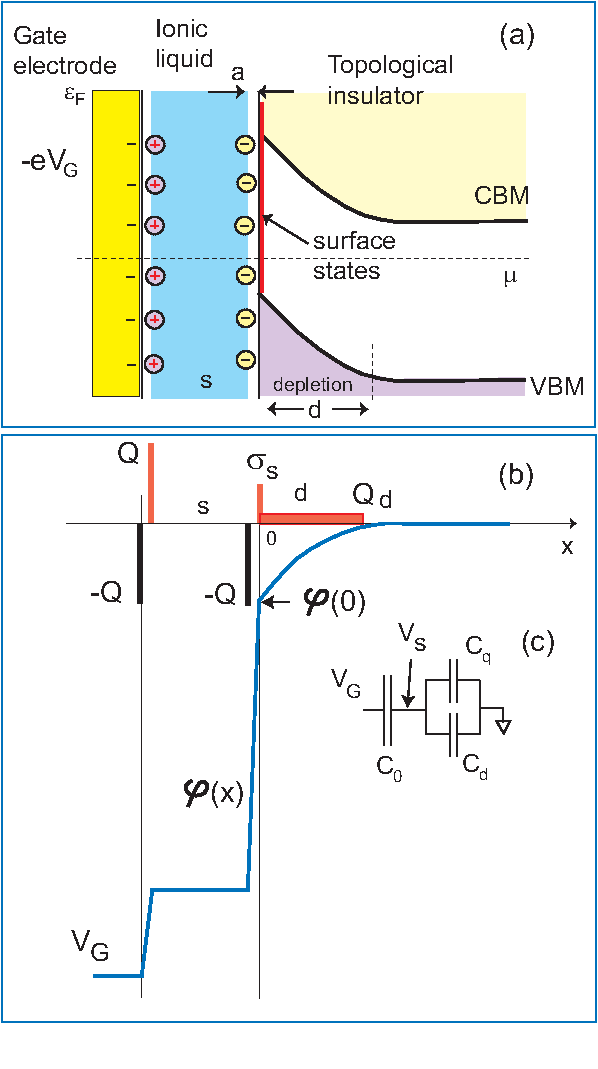
\includegraphics[width=0.65\linewidth]{ch-liquid/figures/FigGate.pdf}
\caption{\label{figGate} 
Sketch of band bending and the profiles of $\rho(x)$ and $\varphi(x)$ in the liquid gating experiment.
Panel (a) shows upwards bending of the bands induced by a negative gate voltage $V_G$. The cations and anions 
define two serial capacitors with spacing $a$ (molecular radius). The depletion layer in the bulk of the TI extends
a distance $d$. Panel (b) displays the charge distribution versus $x$. The negative charge $-Q$ on the gate electrode is
replicated by the anion layer separated by $a$ from the TI surface. This is compensated by the sum of the surface charge density
$\sigma_s$ and the ionized impurity charges inside the depletion layer. The electric potential $\varphi(x)$ corresponding to
$\rho(x)$ is sketched. Panel (c) shows the circuit of the equivalent capacitors $C_0$, $C_d$ and $C_q$.
}
  \end{center}
\end{figure} 



We also sketch the profiles of the charge density $\rho(x)$, the 
electrostatic potential $\varphi(x)$ (the $x$-axis is normal to the surface) and the effective capacitance configuration in Fig. \ref{figGate}b. 
The charge density $\rho(x)$ of the cations and anions in the ionic liquid can be regarded as
delta functions of strength $\pm Q$. In the TI sample, the surface charge density can also be represented by
a delta function ($\sigma_s$). Within the bulk, however, $\rho(x)$ is distributed 
over the depletion layer to a depth $d$. Here we adopt the usual approximation, 
where $\rho(x)$ is taken to be uniform for $0<x<d$. 
As a result, due to the uniform-charge approximation, $\varphi(x)$ varies as $-(x-d)^2$ in the depletion region.
At the surface $\varphi(0)$ becomes
\be
\varphi(0) = -N_ded^2/(2\epsilon_0\epsilon_s),
\label{phi0}
\ee
where $N_d$ is the donor impurity concentration and $\epsilon_s$ the screening dielectric parameter.
The charge $Q_d$ induced in the depletion width by $\varphi(0)$ defines the depletion capacitance
$C_d = N_dedA/\varphi(0) = \epsilon_0\epsilon_s A/d$. The surface charge density $\sigma_s$ 
induced by $\varphi(0)$ is represented by the quantum capacitance
$C_q = \sigma_s/\varphi(0) = e^2(dn_s/d\mu)$. Clearly, $C_d$ and $C_q$ are in parallel
combination (Fig. \ref{figGate}c).

The large slope change at $x=0$ mainly reflects the strong dielectric screening in the bulk of the
TI ($\sigma_s$ makes a negligible contribution). Thus the intense $E$-field produced by the
anions is strongly screened by polarization effects inside the crystal ($E(0^-)\gg E(0^+)$). 
As shown in Fig. \ref{figGate}c, the parallel combination of $C_d$ and $C_q$ is in 
series with $C_0$, the series combination of the cation and anion capacitances.
In all samples, we find that $C_d\gg C_q$, so we may ignore the quantum capacitance in the discussion below.

%\noindent
%\emph{Magnitude of $C_d$}\\
We analyze the magnitudes of the capacitors in Fig. \ref{RvsVG} as below. Fig. \ref{figIndexError}b shows that $E_F$ in Sample 1 decreases by $\sim$100 meV when the applied $V_G$ is -2 V.
Thus, most of the gate voltage drops in the liquid and only a small fraction ($\sim 1/20$) of the applied gate voltage is effective in bending the band ($V_s$ = -0.1 V).
Then we may estimate the depletion capacitance $C_d$ with the $C_0$, which could be assessed by the properties of the ionic liquid.
The value of $C_0/A$ for ionic liquids is approximately 11-12 $\mu$F/cm$^2$~\cite{Koch}.
It is obtained from the standard expression for capacitance, $C_0/A = \epsilon_0\epsilon_{liq}/a$, using $\epsilon_{liq}$ = 4, and $a$ = 3 $\rm\AA$. With the ratio $V_s/(V_G-V_s)\sim C_0/C_d$ (neglecting $C_q$), we estimate that $C_d/A\simeq$ 240 $\mu$F/cm$^2$.

Another method to estimate $C_d$ is by leveraging our observation of the charge flow in the gating experiment. As discussed in the appendix, we measure the ionic gating current when applying the gate voltage, and then integrate the ionic current over time to find the charge $Q$.
For Sample 1 with $V_G$ = -2 V, the ionic charge current deposits a total negative ionic charge at the surface equal to
$-Q/A\sim 2\times 10^{14}e$/cm$^2$ = -3.2$\times 10^{-5}$ C/cm$^2$. 
We notice that $Q/A$ is stored in $C_d$ by the voltage $V_s\sim$ 0.1 V,
so we have $C_d/A\sim$ 320 $\mu$F/cm$^2$, which is 33$\%$ larger than the first estimate. This error is still within our uncertainties since the inaccurate measurement of the actual area coated by the anions can provide the main source of the uncertainty. In our experimental setup, the ions can coat the silver paint contacts and voltage and current leads, and the area can exceeds that of the crystal $A$ by 50 to 100$\%$.

Using $\frac Q A = N_d e d + \sigma_s$, we can estimate the depletion width $d$ in our Bi$_2$Te$_2$Se crystal.
The donor density $N_d$ is roughly equal to the bulk density observed at 4 K, $n_b~\sim 2\times 10^{17}$ cm$^{-3}$.
This gives $d\simeq$ 10 $\mu$m, suggesting a thick depletion layer. We notice that the deep penetration of the depletion region into the bulk
is consistent (within a factor of 2) with the 40$\%$ change observed in the resistivity and Hall coefficient at 4 K.

From the range of $C_d/A$ (240-320 $\mu$F/cm$^2$), we find that the depletion capacitance in our Bi$_2$Te$_2$Se sample is 5,000-6,000$\times$ larger than the values commonly observed in a Si-MOSFET device ($C_{d,Si}/A\simeq$ 0.05-0.06 $\mu$F/cm$^2$~\cite{SternRMP,Sze}).
Such a giant enhancement in TI indicates a very large polarizability in its ground state when $E_F$ lies inside the energy gap. A possible underlying reason is the impurity band in Bi$_2$Te$_2$Se while energy gap in high-purity Si is devoid of impurity states. There is evidence for the impurity band in Bi$_2$Te$_2$Se in many experiments\cite{Ando10}. For example, the $\rho-T$ curve of
Bi$_2$Te$_2$Se at 4 K displays a small, but metallic conductivity possibly arising from a large population of impurity-band electrons.


In addition, we hope to make a comment on the finite DOS in the gap here.
In order to create an extended depletion region with significant band bending and a thick depletion layer, as we discuss above and show in Fig. \ref{figGate}a, 
the weak bulk conductivity must be further driven to zero throughout the depletion region
in order to sustain a finite $E$-field (otherwise one has Thomas-Fermi screening with the very short screening length 
$\lambda_{TF} \simeq$ 6 $\rm\AA$
for $n_b$ = 2$\times 10^{17}$ cm$^{-3}$m). This looks a little surprising at the first sight. But the existence of a mobility edge in the 
impurity band can explain how band-bending is sustained over a large depletion region without inducing the Thomas-Fermi screening. If $E_F$ lies below the mobility edge throughout the depletion layer,  then the bulk conductivity there will vanish at 4 K. Besides, because impurity-band states close to the mobility edge have a greatly enhanced polarizability in an $E$-field, we expect the electronic contribution to 
dielectric constant $\epsilon_s$ to be orders of magnitude larger than the lattice contribution. Our measurements of $C_d/A$ probe directly the electronic polarizability in the depletion region. We will discuss a possible scenario is described in the appendix.


\section{Discussion and Summary}
\label{sec:liquid:discussion}

We have tuned the $E_F$ of the surface Dirac fermions over a considerable range, by applying the novel ionic liquid gating technique to the insulating Bi$_2$Te$_2$Se crystals with $\rho >$ 4 $\Omega$cm at 5 K.
In contrast to previous gating experiments, we readily resolve prominent surface SdH oscillations 
at each gating voltage. From the SdH periods, we find that the surface Fermi energy $E_F$
(Sample 1) decreases  
from 180 mV to 75 mV above the Dirac Point as $V_G$ is changed from 0 to -2.8 V. 
In a 14 T magnetic field, the lower limit corresponds to
the middle of the broadened $N$ = 1 Landau Level. Attaining such low Landau levels enables the $-\frac12$
intercept (predicted for Dirac fermions) to be determined with high accuracy.
Furthermore, the intercepts are closely similar for a broad range of $V_G$ in both Samples 1 and 2, adding more evidence for a $\pi$ Berry phase of the surface Dirac electrons on Bi$_2$Te$_2$Se.

Through analyzing the SdH oscillations, we also obtain the surface mobility $\mu_s$ and density $n_s$ for the surface states. And our calculation shows that the Hall conductivity from the surface Dirac fermions exposed to the anions accounts
for up to 83$\%$ of the total observed weak-$B$ Hall conductivity at 5 K. Such a large proportion is mainly caused by the large difference between the surface and the bulk mobilities. Combining these parameters with a semi-classical two-band model, we obtain an accurate determination
of the bulk carrier mobility and density at each $V_G$ (Fig. \ref{figHall}). We find that the surface carrier density $n_s$ decreases steeply while the surface mobility
$\mu_s$ increases to a maximum value of 2,400 cm$^2$/(Vs) under gating. The bulk carriers are depleted to a depth of 10 $\mu$m from the 
surface, with $\mu_b$ remaining at the low value of 20 cm$^2$/(Vs).



The large enhancement of $\mu_s$
by liquid gating (Fig. \ref{figHall}b) is perhaps the most intriguing 
feature in our ionic liquid gating experiments. To our knowledge, this is the first realization of 
enhancement of surface SdH amplitudes by an \emph{in situ} technique, and may provide a way to improve the surface conductivity. A clue for the explanation arises from an STM experiment~\cite{Beidenkopf2011}, which reveals that
the Dirac Point closely follows spatial fluctuations of the local
potential on length scales of 30-50 nm. Such a large fluctuation in the surface band can lead to strong scattering
of surface electrons and then reduces the surface mobility. We speculate that, under liquid gating, the anions accumulate
at local maxima in the potential, thereby leveling out the strongest spatial fluctuations and improving the electron lifetime.
The results are encouraging and indicate that alternative routes that even out local
potential fluctuations can further improve $\mu_s$. This could be important for future applications and devices.

We also provide analysis and experimental data in order to uncover whether the ionic liquid gating actually alters the carrier concentration by chemical
reactions or simply through bending the band. 
By carefully selecting the experimental conditions (e.g. the gating temperature),
monitoring charge accumulated $Q$, and checking for reversibility, we establish that band-bending is the dominant effect
in our experiments. Lastly, the five quantities measured at each gate voltage setting ($E_F$, $n_s$, $n_b$, $\rho$ and $Q$)
provide a quantitative picture of the gating process and the band bending effect. The depletion
capacitance measured implies that, within the depletion region, the electronic polarizability is strongly enhanced.



\chapter{Anomalous Conductivity Tensor and Chiral Anomaly in the 3D Dirac Semimetal Na$_3$Bi\label{ch:na3bi}}
%A review ~\cite{Yang2014}

%Introduce a little about the Hamiltonian and Xi Dai's theory about Na3Bi

In this chapter we will discuss our transport experiments on the 3D Dirac semimetal Na$_3$Bi. The 3D Dirac semimetal is a three dimensional analog of graphene, with its Dirac node protected against gap-open hybridization. Previous first-principle calculations~\cite{Wang2012} have predicted that both Na$_3$Bi and Cd$_3$As$_2$ are 3D Dirac semimetals in which the Dirac nodes are protected by crystal symmetries. In particular, $C_3$ symmetry prevents the gap opening in Na$_3$Bi. Thus such Dirac nodes in Na$_3$Bi are formed by overlapped Weyl nodes. Also, photoemission experiments have confirmed the linear dispersion in the bulk band and the Fermi arcs on its surface~\cite{Liu2014a, Xu2015, Xu2013}, as shown in Fig. \ref{figNa3Bi_band}(B) and (D). In a magnetic field, the protected nodes of the Dirac semimetal could be sensitive to the breaking of time-reversal invariance and become a Weyl semimetal~\cite{Wang2012}. Many groups~\cite{Son2013,Burkov2011,Hosur2013,Parameswaran2014} predict that, in Dirac and Weyl semimetals, the chiral anomaly effect can lead to many new transport properties in an intense magnetic field $\bf B$, such as novel negative longitudinal magnetoresistance, non-local transport and anomalous Hall effect. To search for these phenomena, we have grown two types of Na$_3$Bi crystals, which have different Fermi levels. And we find that they display very interesting but different transport properties. 

\begin{figure}[!htbp]
  \begin{center}
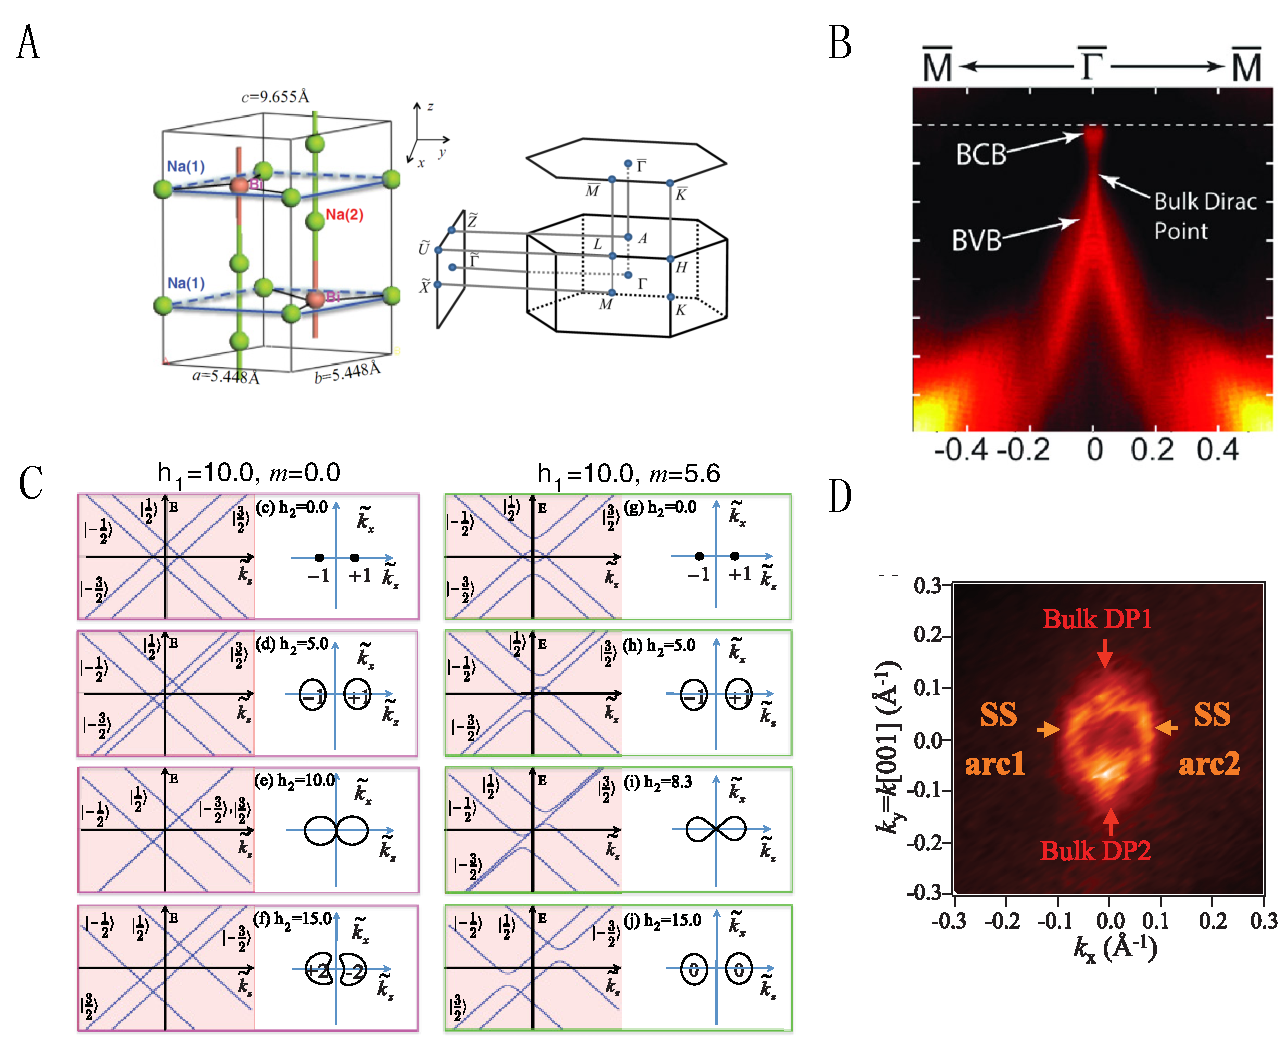
\includegraphics[width=1\linewidth]{ch-na3bi/figures/Na3Bi_band.pdf}
\caption{\label{figNa3Bi_band} The crystal and band structures of Na$_3$Bi. Panel (A) displays the crystal structure and a sketch of the first Brillouin zone of Na$_3$Bi \cite{Wang2012}. Panel (B) shows the linear-dispersed 3D bulk bands from the ARPES experiment \cite{Liu2014a}. It confirms the 3D Dirac nature of Na$_3$Bi. Panel (C) depicts the phase diagram of Na$_3$Bi with different mass terms \cite{Wang2012}. It explains the conditions under which the underlying Weyl branches are separated in momentum space or a gap opens. Panel (D) shows the surface Fermi arcs on Na$_3$Bi in an ARPES experiment \cite{Xu2015}. Fermi arcs are predicted to connect two Weyl nodes, and are signatures of a WSM or DSM. Thus this experimental discovery provides strong support for the theory of the WSM and DSM.
}
  \end{center}
\end{figure}

The first type we discuss below has a high $E_F$, which exhibits robust anomalies both in the conductivity and the resistivity when a magnetic field is applied\cite{Xiong2015a}. Specifically, the magnetoresistance follows a $B$-linear shape up to 35 T, while the Hall angle displays an unusual profile approaching a step-function at high fields. Moreover, the conductivities $\sigma_{xx}$ and $\sigma_{xy}$ follow the same power-law in their field dependence when B is large. These findings are unexpected from the conventional transport theory and may arise from a transport lifetime that is very sensitive to the magnetic field. Besides, we also have observed prominent quantum oscillations both in magnetoresistance and the torque magnetometry experiment. Such large oscillations provide an accurate measurement of the Fermi surface and indicate a high mobility in our samples.
%Besides, we also provide some evidence that the Fermi surface may be composed of two distinct valleys, indicating that the Fermi energy may lie below the Lifshitz transition of the bulk Dirac bands.

Our other type of Na$_3$Bi crystals has a much lower chemical potential ($E_F \sim 30$ meV above the Dirac point). As a result, when the Dirac point is split into two chiral Weyl nodes by breaking the time-reversal symmetry in a magnetic field, the proposed charge pumping between the Weyl nodes could be uncovered in transport experiments\cite{Xiong2015b}. This effect is a condensed-matter version of Adler-Bell-Jackiw anomaly ~\cite{Nielsen1983,Wan2011,Burkov2011, Hosur2013} investigated in quantum field theory and high energy physics. Pioneering theoretical work has predicted that charge could flow between the Weyl nodes when an electric field $\bf E$ is applied $\parallel \bf B$, and its strength is determined by $\bf E\cdot \bf B$. Son et. al. ~\cite{Hosur2013} found that with the semiclassical scattering term, the longitudinal conductance in a magnetic field will be enhanced quadratically by the chiral anomaly effect. We will discuss in this chapter our observation of a novel, negative and highly anisotropic magnetoresistance in the Dirac semimetal Na$_3$Bi. We find that the novel negative MR is acutely sensitive to the angle between $\bf B$ and $\bf E$, and is incompatible with conventional transport. To compare with the theoretical prediction, we also rotate both $\bf E$ and $\bf B$, and find that it qualitatively confirms the prediction of the chiral anomaly effect in a semimetal. 



% include other files for sections of this chapter. These use the 'input' command since each section within a chapter should not start a new page.
% If you want to swap the order of sections, it is as simple as reversing the order you include them. 
\section{Linear Magnetoresistance in Na$_3$Bi with a High Chemical Potential}
\label{sec:na3bi:lmr}


Na$_3$Bi belongs to the space group P6$_3$/mmc and its lattice parameters are a = 5.448 $\rm{\AA}$ and c = 9.655 $\rm{\AA}$. It has a simple crystal structure with three distinct crystallographic sites: Na(1), Na(2), and Bi. It consists of Na(1)-Bi honeycomb layers stacked along the c axis, with Na(2) between the layers. Our first attempt to grow Na$_3$Bi crystals by slowly cooling a stoichiometric melt resulted in crystals with a lot of Na vacancies. As a result, they are mixed with the superconducting NaBi phase. To suppress these defects, we then used Na-rich compositions (90$\%$ and 95$\%$) and the flux-grow method \cite{Kushwaha}. We have obtained high-quality Na$_3$Bi crystals whose structure has been confirmed by X-ray diffraction (the lattice structure is sketched in Fig. \ref{figR}C). The crystals are deep purple and in an elongated hexagonal shape as shown in the inset of Fig. \ref{figR}A. Their largest facets are normal to the $c$-axis (001). Na$_3$Bi crystals are very fragile in any amount of water or oxygen. We find that they can be easily oxidized completely within 30 seconds in exposure to air. This has been a large obstacle to our sample mounting process. To protect the sample from any oxidization, we need to attach the contacts to the crystals with Ag epoxy inside an Ar glovebox and then cover the sample with paratone oil and seal it. Only after all these steps, we can safely load the sample into the cryostat (see the details in previous chapters). The resistance v.s. temperature curve (Fig. \ref{figR}A) of Na$_3$Bi shows a metallic behavior with the 4K resisitivity ranging from 1.72 to 87 $\mu\Omega$cm. Fig. \ref{figR}B shows the Hall effect which is linear and $n$-type. Fig. \ref{figR}A also indicates a nearly $T$-independent Hall coefficient $R_H = \rho_{yx}/B$ ($\bf\hat{x}||I$ and $\bf\hat{z}||\hat{c}$, where $\bf I$ is the current). We have measured several different batches of the crystals. Among them, Batch B and C were not annealed, while Batch G was annealed for one month. 

The typical MR curves of Na$_3$Bi at selected angles are shown in Figure \ref{figR}C. The tilt angle $\theta$ is between $\bf\hat{c}$ and the field ${\bf H}={\bf B}/\mu_0$, with $\mu_0$ the vacuum permeability). Here $\theta$ is defined as the angle between $\bf B$ and the $c$-axis of the sample. The current flows within the $a-b$ plane. The current and $\bf B$ are parallel when $\theta \equiv 90^\circ$. The MR profiles are linear in all angles, and their MR ratios reaches the maximum at $\theta \equiv 0^\circ$ while decreasing with $\bf H$ tilted into the $a$-$b$ plane ($\theta\to 90^\circ$). 

\begin{figure}[!htbp]
  \begin{center}
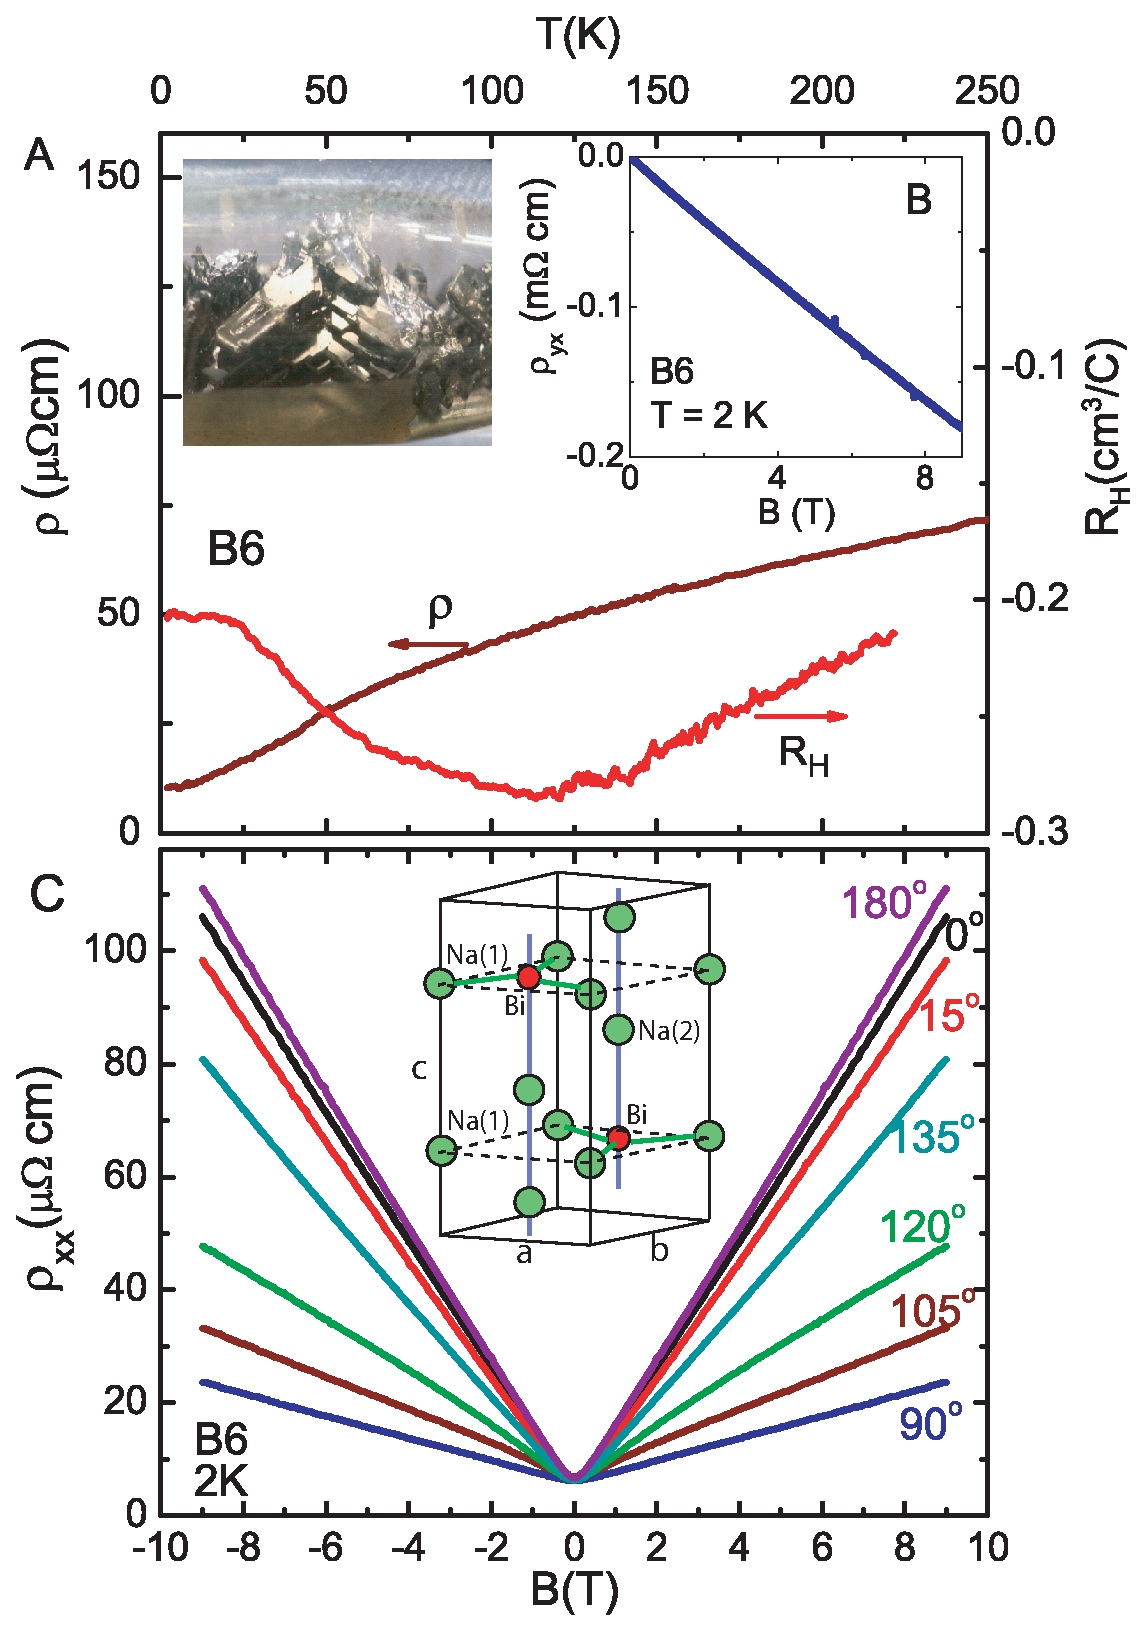
\includegraphics[width=0.8\linewidth]{ch-na3bi/figures/FigRMRA}
\caption{\label{figR}
Magnetotransport in Na$_3$Bi. Panel A: The zero-field resistivity $\rho$ and the Hall coefficient $R_H$ v.s. $T$ (measured with $\bf H||c$). Inset shows the crystals sealed in a vial. The largest facet is normal to $\bf\hat{c}$. Panel (B) shows the Hall resistivity $\rho_{yx}$ v.s. $B$ measured at 2 K in Sample B6.
Panel (C): The $H$-linear magnetoresistance in Sample B6 measured at 2 K at selected tilt angles $\theta$ to $\bf\hat{c}$. The MR ratio is largest at $\theta=0^\circ$ (and 180$^\circ$). (${\bf B} = \mu_0 {\bf H}$ with $\mu_0$ the vacuum permeability). The crystal structure of Na$_3$Bi is sketched in the inset (adapted from Ref.~\cite{Liu2014a}). 
}
  \end{center}
\end{figure}

Figure \ref{figR}C also displays quantum oscillations in MR curves, although they are not very large in amplitudes. After subtracting a smooth background from the MR data, we find that all the samples display clear Shubnikov de Haas (SdH) oscillations in $\rho_{xx}(B)$. The SdH oscillations provide an accurate way ($\pm3\%$) to measure the Fermi Surface cross-section $S_F$ and the Fermi wavevector $k_F$. In addition, we have measured the de Haas van Alven (dHvA) oscillations in the magnetic susceptibility with the torque magnetometry technique. The quantum oscillations in the torque measurement are much more prominent than those in MR and can yield information about the sample with high precision. Figure \ref{figtorque}A shows the oscillatory component of the magnetization together with a fit to the standard Lifshitz-Kosevich (LK) expression. The fitting quality is quite good, and it yields a Fermi surface area around 200 T. It corresponds to a bulk carrier density $n = g_vk_F^3/3\pi^2$ (with the valley and spin degeneracies $g_v$ and $g_s$ both equal to 2) that ranges from 2.6-4.1$\times 10^{19}$ cm$^{-3}$, consistent with the Hall effect (Table \ref{tab}). By fitting to the dHvA amplitudes v.s. $1/H$ and $T$ curves (Panels B and C), we can obtain the effective mass $m^* = 0.11 m_0$ ($m_0$ is the free electron mass),  the Fermi velocity $v_F = 8.05\times10^5$ m/s and the quantum lifetime $\tau_Q=8.16\times10^{-14}$ s. We also tilted the direction of $\bf B$ in both our MR and torque magnetometry experiments, in order to measure the anisotropy of the Fermi surface. Interestingly, as displayed in Fig. \ref{figtorque}D, the frequencies of the oscillations at different angles do not vary much and they suggest that the FS cross section $S_F$ is nearly spherical. 

\begin{figure}[!htbp]
  \begin{center}
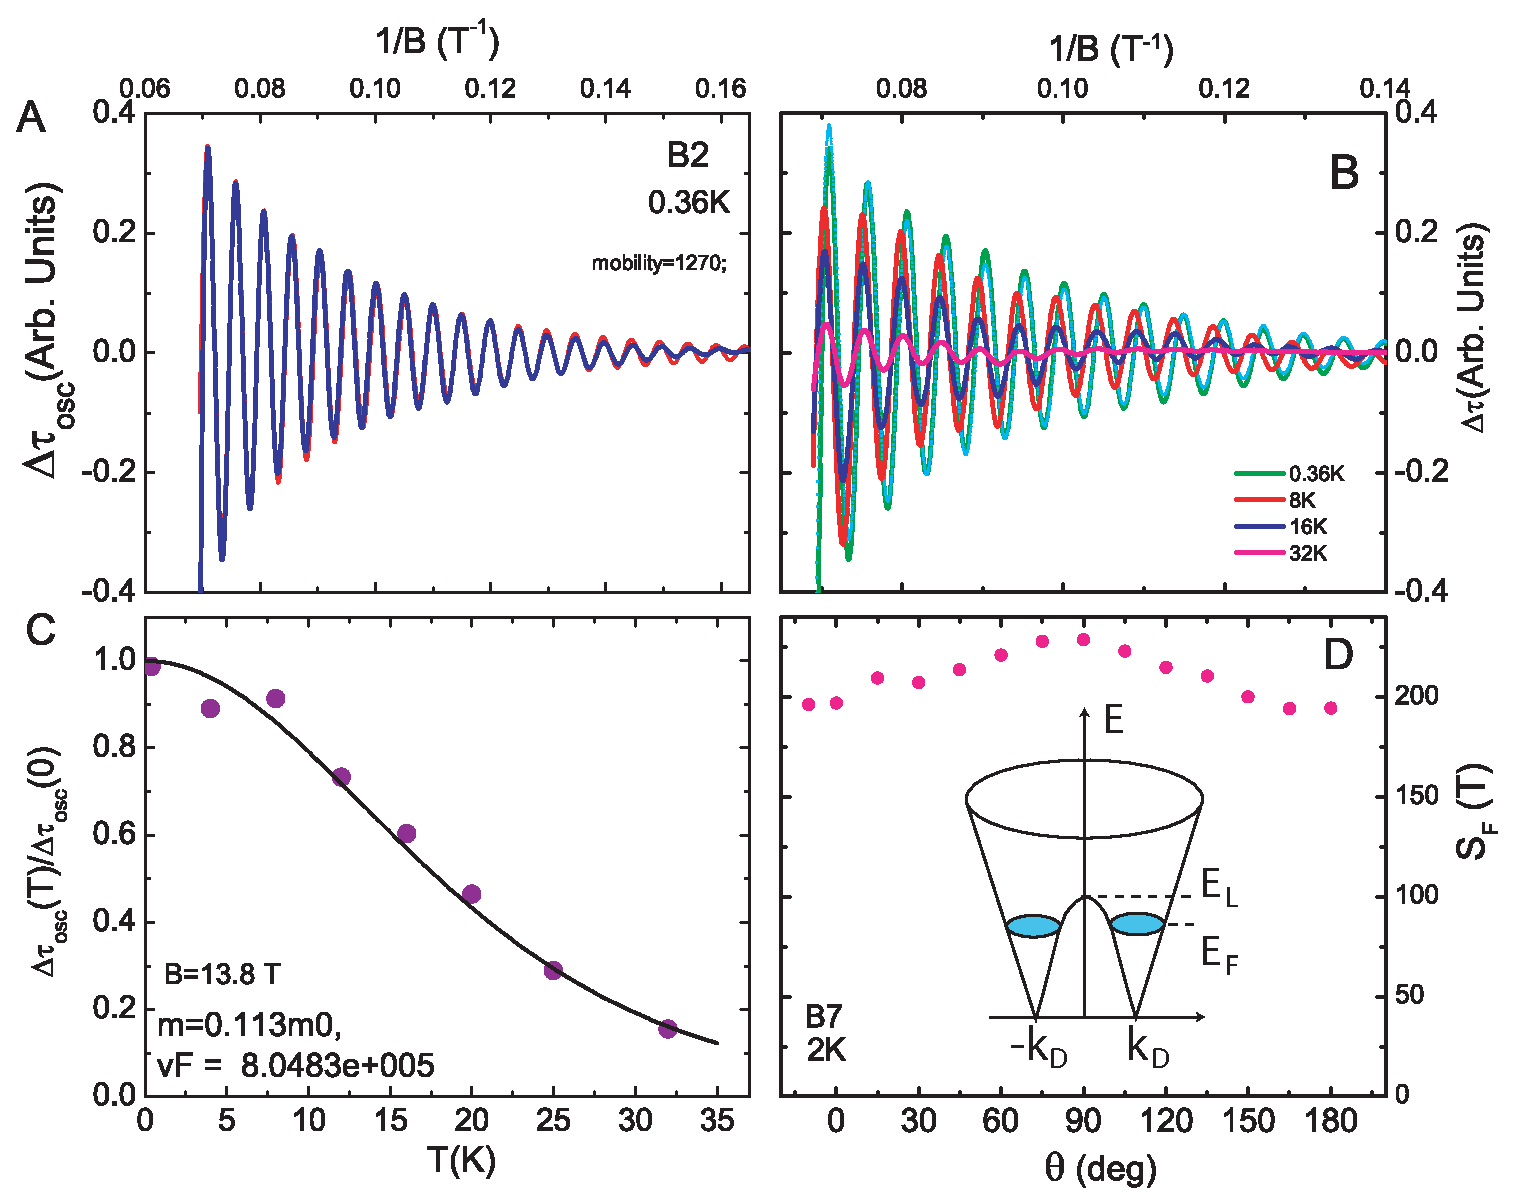
\includegraphics[width=1\linewidth]{ch-na3bi/figures/FigTorqueA}
\caption{\label{figtorque} (Color online)
Torque measurements of the de-Haas van Alven (dHvA) oscillations in Na$_3$Bi. The dHvA oscillations (solid curve in Panel A) can be fit well to the LK expression (dashed curve) with one period. From the damping versus $H$ (Panel A) and the $T$ dependence (Panels B and C), we obtain the Fermi surface section $S_F$, the effective mass $m^* = 0.11 m_0$ ($m_0$ the free mass), velocity $v_F$ = 8.05$\times 10^5$ m/s, and $\tau_Q$ = 8.16$\times 10^{-14}$s. The plot of the peak fields $B_{min}$ and $B_{max}$ vs. the integers $N$ (Panel D) yields $S_F$. 
}
  \end{center}
\end{figure}

We notice that previous Na$_3$Bi samples measured by ARPES experiments~\cite{Liu2014a, Xu2015, Xu2013} all have a chemical potential below the Dirac point. And it has hidden the information about the conduction band. In our crystals, by suppressing the Na vacancies, we have obtained crystals with $E_F$ in the conduction band, as implied by the $n$-type sign of the Hall resistivity $\rho_{yx}$. The band calculations~\cite{Wang2012} predicted the existence of two Dirac nodes centered at $(0,0,\pm k_D)$ caused by gap inversion (sketch in Fig. \ref{figtorque}D). When the energy rises following the conduction band, the two Dirac cones will eventually meet and merge into one band when the energy exceeds the Lifshitz-transition energy $E_L$. Recent ARPES experiments have confirmed the predicted dispersion and measured $k_D$ to be around 0.095 $\rm{\AA}^{-1}$~\cite{Liu2014a} and 0.10 $\rm{\AA}^{-1}$~\cite{Xu2013} (see also~\cite{Zhang2014}). But the ARPES data of the conduction band is lacked, and it cannot tell where $E_L$ is in the conduction band. An important question is whether $E_F$ in our samples lies above or below $E_L$, since $E_F$ in our sample is already quite high. We also notice that if the merged bands above $E_L$ are also isotropic, then the Fermi wave vector $k_F$ of the outer merged pocket will be larger than $k_D$ when $E_F > E_L$. On the other side, if $k_F$ is much smaller than $k_D$, then we will have  $E_F < E_L$. As shown in Table \ref{tab}, our measured $k_F$ ranges from 0.073 to 0.084 $\rm{\AA}^{-1}$. As these values are similar to but a little smaller than $k_D$, suggesting a possibility that $E_F$ lies below $E_L$. But if the merged bands are anisotropic, it's still possible that $E_F$ is slightly higher than $E_L$. This issue is worth exploring for both ARPES and transport study, and it may require crystals with a higher quality.

If $E_F < E_L$, then the FS consists of two Dirac valleys on the opposite sides of the $\Gamma$ point in the Brillouin zone, i.e. $g_v = 2$. If $E_F > E_L$, there will also be two Fermi pockets with one enclosing another. In the first case, the two Fermi surface areas will be similar but may have a small difference due to the inhomogeneity in the sample. In the second case, the two Fermi pockets will have different $S_F$, and the difference varies with $E_F$. Interestingly, We also notice that there is a persistent weak beating behavior in the SdH oscillations in many of our samples, as shown by the data of five samples in Fig. \ref{figBeats}A. Fourier transform analysis of these oscillations suggest that there are two main frequencies $f_1$ and $f_2$ corresponding to two values of $S_F$ differing by $\sim 16\%$. Such beating pattern may indicate the quantum interference between the two orbits on the two Fermi pockets. But we may need to carry out more detailed studies on such interference in the future.

\begin{figure}[!htbp]
  \begin{center}
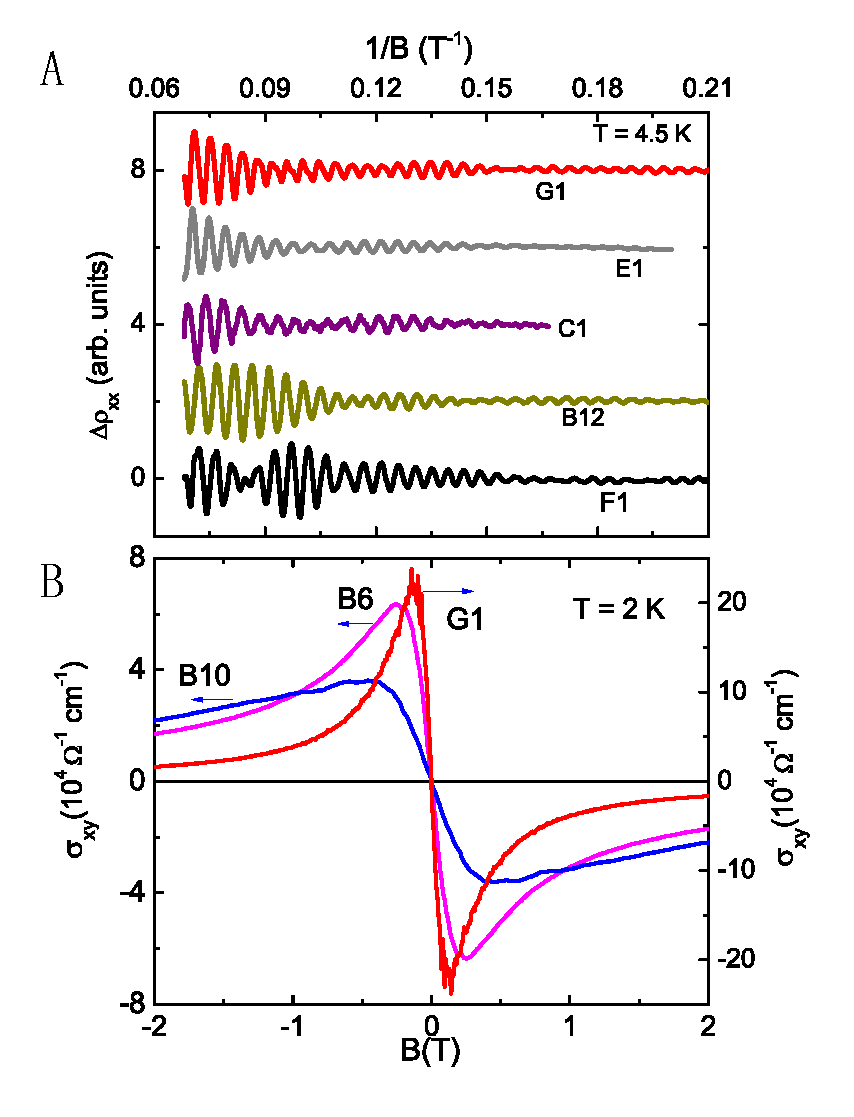
\includegraphics[width=0.9\linewidth]{ch-na3bi/figures/FigBeatsDrude.pdf}
\caption{\label{figBeats} 
Panel A: Curves of $\Delta\rho_{xx}$ showing modulation of the SdH amplitudes in different Na$_3$Bi samples. The beating pattern implies a small splitting of the fundamental SdH frequency.
Panel B compares the Hall conductivity $\sigma_{xy}(B)$ in 3 samples at 2 K. In the 3 curves, the peak field $\pm B_{\mu}$ yields the values $\mu$ = 21,640, 39,250 and 91,000 cm$^2$/Vs in B10, B6 and G1, respectively.
}
  \end{center}
\end{figure}

As reported in \cite{Liang2015}, there could be a strong suppression of backscattering in Dirac semimetals. Therefore it is of great value to investigate both the transport lifetime $\tau_{tr}$ and the quantum lifetime $\tau_Q$ in Na$_3$Bi. The conventional way to obtain $\tau_{tr}$ is from the ratio of $\rho_{yx}/\rho_{xx}$, but it requires very accurate measurement of sample dimensions. Since we mount our Na$_3$Bi samples in the glove box and the thickness measurement is not accurate, the calculated $\tau_{tr}$ by this method will have a large error bar. Instead, we leverage the Drude formula for $\sigma_{xy}$ to find $\tau_{tr}$. By the Bloch-Boltzmann theory, the extrema in $\sigma_{xy}(B)$ occur at the peak fields $\pm B_\mu$, where $1/B_\mu$ equals the ``Hall mobility'' $\mu_H$. Fig. \ref{figBeats}B shows the typical $\sigma_{xy}(B)$ curves of three samples which have the characteristic dispersion-resonance profile produced by cyclotron motion of the carriers. The $\sigma_{xy}(B)$ curves are derived by inverting the measured resistivity matrix $\rho_{ij}(B)$. As displayed in Fig. \ref{figBeats}B, the mobilities from Sample B10 ($\mu$ = 21,640 cm$^2$/Vs) to B6 (39,250 cm$^2$/Vs) and G1 (91,000 cm$^2$/Vs), increase as the peak field $B_{\mu}$ decreases. We will discuss below the influences on the Hall angle profiles from different $\mu_H$. With $\mu = ev_F\tau_{tr}/\hbar k_F$, we find that the transport lifetime $\tau_{tr}$ exceeds $\tau_Q$ by a ratio $R_{\tau}$ = 10-20 ($R_{\tau}$ is expected to exceed 1 since $\tau_Q$ reflects broadening due to all scattering processes). As a comparison, $R_{\tau}$ in Cd$_3$As$_2$ is as large as 10$^4$~\cite{Liang2015}. 




%In the relaxation-time $\emph{ansatz}$, the Boltzmann equation describing changes to the distribution function $f_{\bf k}$ caused by an electric 
With the relaxation-time approximation, the Boltzmann equation that describes the change of the distribution function $f_{\bf k}$ in an electric 
field $\bf E$ is expressed as~\cite{Ziman}
\be
e{\bf E\cdot v}\frac{\partial f^0_{\bf k}}{\partial E_{\bf k}}  
+ e{\bf v\times B\cdot}\frac{\partial g_{\bf k}}{\partial {\bf k}}
= -\frac{g_{\bf k}}{\tau_{tr}},
\label{Boltz}
\ee
where $e$ is the elemental charge and $g_{\bf k} = f_{\bf k}-f^0_{\bf k}$, with $f^0_{\bf k}$ the Fermi-Dirac function. $E_{\bf k}$ and the velocity $\bf v$ are, respectively, the energy and velocity at state $\bf k$. Then the conductivity tensor $\sigma_{ij}$ is
\be
\sigma_{xx} = ne\mu/D, \quad\quad \sigma_{xy} = ne\mu^2B/D,
\label{sxx}
\ee
where $D = 1+(\mu B)^2$. We notice that the ratio $\sigma_{xy}/\sigma_{xx}= \mu B$, which is the Hall angle $\tan\theta$, is linear in $B$. When the conductivity matrix is converted to the resistivity matrix, the above $\emph{ansatz}$ yields a $B$-independent $\rho_{xx}$. This is because the Hall electric-field $E_y$ exactly balances the Lorentz force. Moreover, we can obtain $\sigma_{xx}\sim 1/B^2$ and $\sigma_{xy}\sim 1/B$ at large $\mu B$. In a material that has two types of carriers with different mobilities, $\rho_{xx}$ will follow a $B^2$ dependence at low fields and will saturate at high fields. The key assumption underlying these standard predictions is that $\tau_{tr}$ (hence $\mu$) is a constant independent of $B$. This assumption has been firmly established in conventional metals and semimetals in the impurity-scattering regime (elastic scattering). The prediction is a cornerstone of semiclassical transport.


Nevertheless, the observed field dependences of $\sigma_{xx}$ and $\rho_{xx}$ in Na$_3$Bi follow an essentially different profile from the standard predictions while only $\rho_{yx}(B)$ appears conventional. As shown in Fig. \ref{figR}, $\rho_{xx}$ in Na$_3$Bi increases linearly with $B$ without any saturation. In B11 (Fig. ref{figMRtan}), we show that the $B$-linear profile extends to 35 T with no evidence of deviation or saturation. This behavior deviates from the predicted quadratic field dependence. A $B$-linear MR is rare in conventional conductors (see Abrikosov's comments~\cite{Abrikosov1998}. Sometimes it can be caused by open orbits. But here we can exclude the possibility of open orbits~\cite{Ziman}). However, interestingly, there are increasing numbers of examples for a $B$-linear MR in materials with unusual topological phases~\cite{Qu,Liang2015}. To find out whether the $B$-linear MR is universal in Na$_3$Bi crystals with high $E_F$, we have investigated eight samples (Table \ref{tab}). All these samples have a similar MR profile. Figure \ref{figMRtan}A shows that the $B$-linear MR is a very robust feature in Na$_3$Bi. We also notice that the MR ratio (measured at 15 T) could be very different among our samples, as it increases from $\sim 14$ in B10, to $163$ in G1 (the sample with the highest $\mu$). A more detailed test of the correlation between the MR ratio and the sample mobility will be made in the future. 



We also find a dramatic anomaly in the Hall-angle profile. In Fig. \ref{figMRtan}B, we compare the $\tan\theta$ v.s. $B$ curves measured in four samples with an increasing $\mu$, i.e. B10, B12, B6 and G1. In all these samples, $\tan\theta$ initially rises very rapidly in weak $B$ and then saturates to a value independent on the magnetic field. Besides, the slope of the rise at low $B$ depends on the mobility. The samples (B10 and B12) with a low $\mu$ have a gentle rise in $\tan\theta$ while the samples (B6 and G1) with a high $\mu$ have an abrupt rise. In particular, the $\tan\theta$ v.s. $B$ curve in Sample G1 resembles a step function. Since $\tan\theta = \mu B$, if we assume that $\tan\theta$ in Na$_3$Bi has a universal independent behavior starting at weak fields (B$>$0.5 T), then a simple explanation will be a decreasing $\tau_{tr}$ with the increasing B, such as 
\be
\tau_{tr} \sim 1/B.
\label{tau}
\ee



We also notice that Eq. \ref{tau} could also account for the $B$-linear MR profile, i.e. 
$\rho_{xx} = 1/ne\tau_{tr} \sim B.$
Interestingly, Eq. \ref{tau} implies that the high-field $B$ dependence of $\sigma_{xx}$ is reduced by one power of $B$ to $\sigma_{xx}(B)\sim 1/B$ (Eq. \ref{sxx}), but does not modify the field dependence of $\sigma_{xy}$ ($\sigma_{xy}\sim 1/B$). This is because $\mu$ cancels out at large $B$. Therefore both $\sigma_{xx}$ and $\sigma_{xy}$ evolve as $1/B$ at large $B$, generating the step-profile of $\tan\theta$. 

\begin{figure}[!htbp]
  \begin{center}
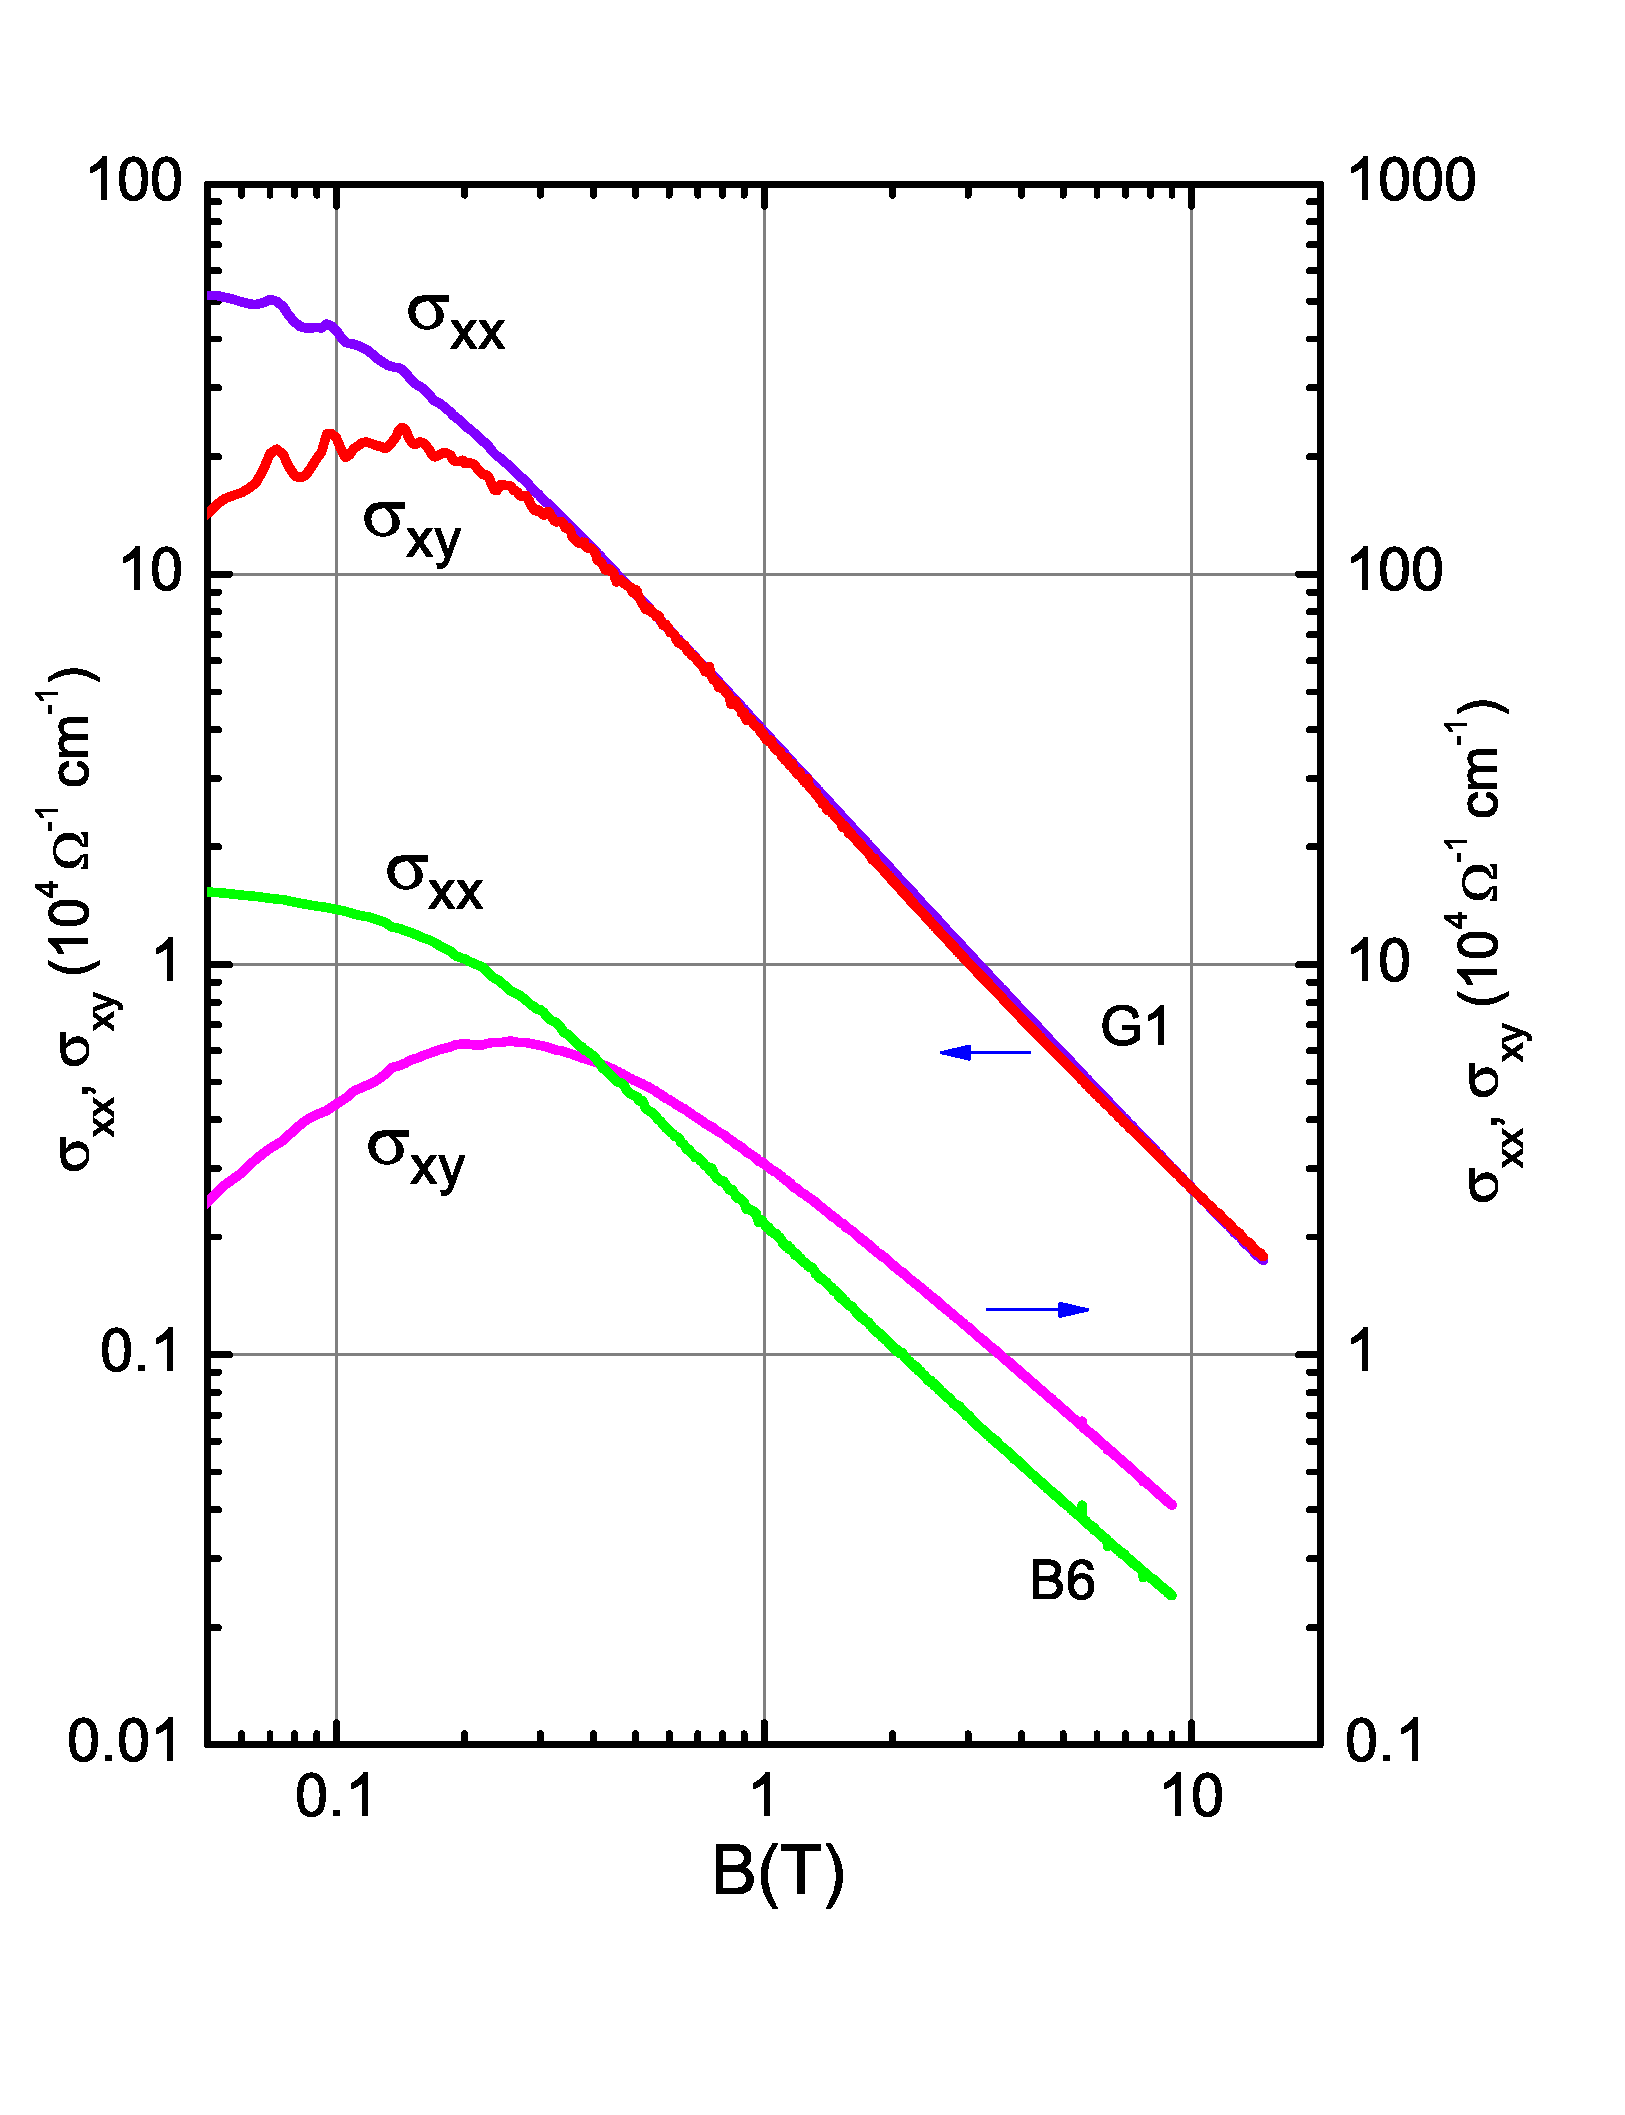
\includegraphics[width=0.8\linewidth]{ch-na3bi/figures/FigLogSigxy}
\caption{\label{figCond} 
Log-log plots of $\sigma_{xx}$ and $\sigma_{xy}$ vs. $B$ in Sample G1 and B6. Consistent with Eq. \ref{tau}, both quantities approach the same power law $B^{-\beta}$ when $B$ exceeds 0.3 and 2 T in G1 and B6, respectively. The measured $\beta$ is 1.15 and 1.0 in G1 and B6, respectively. Curves for B6 are shifted vertically.
}
  \end{center}
\end{figure}



\begin{figure}[!htbp]
  \begin{center}
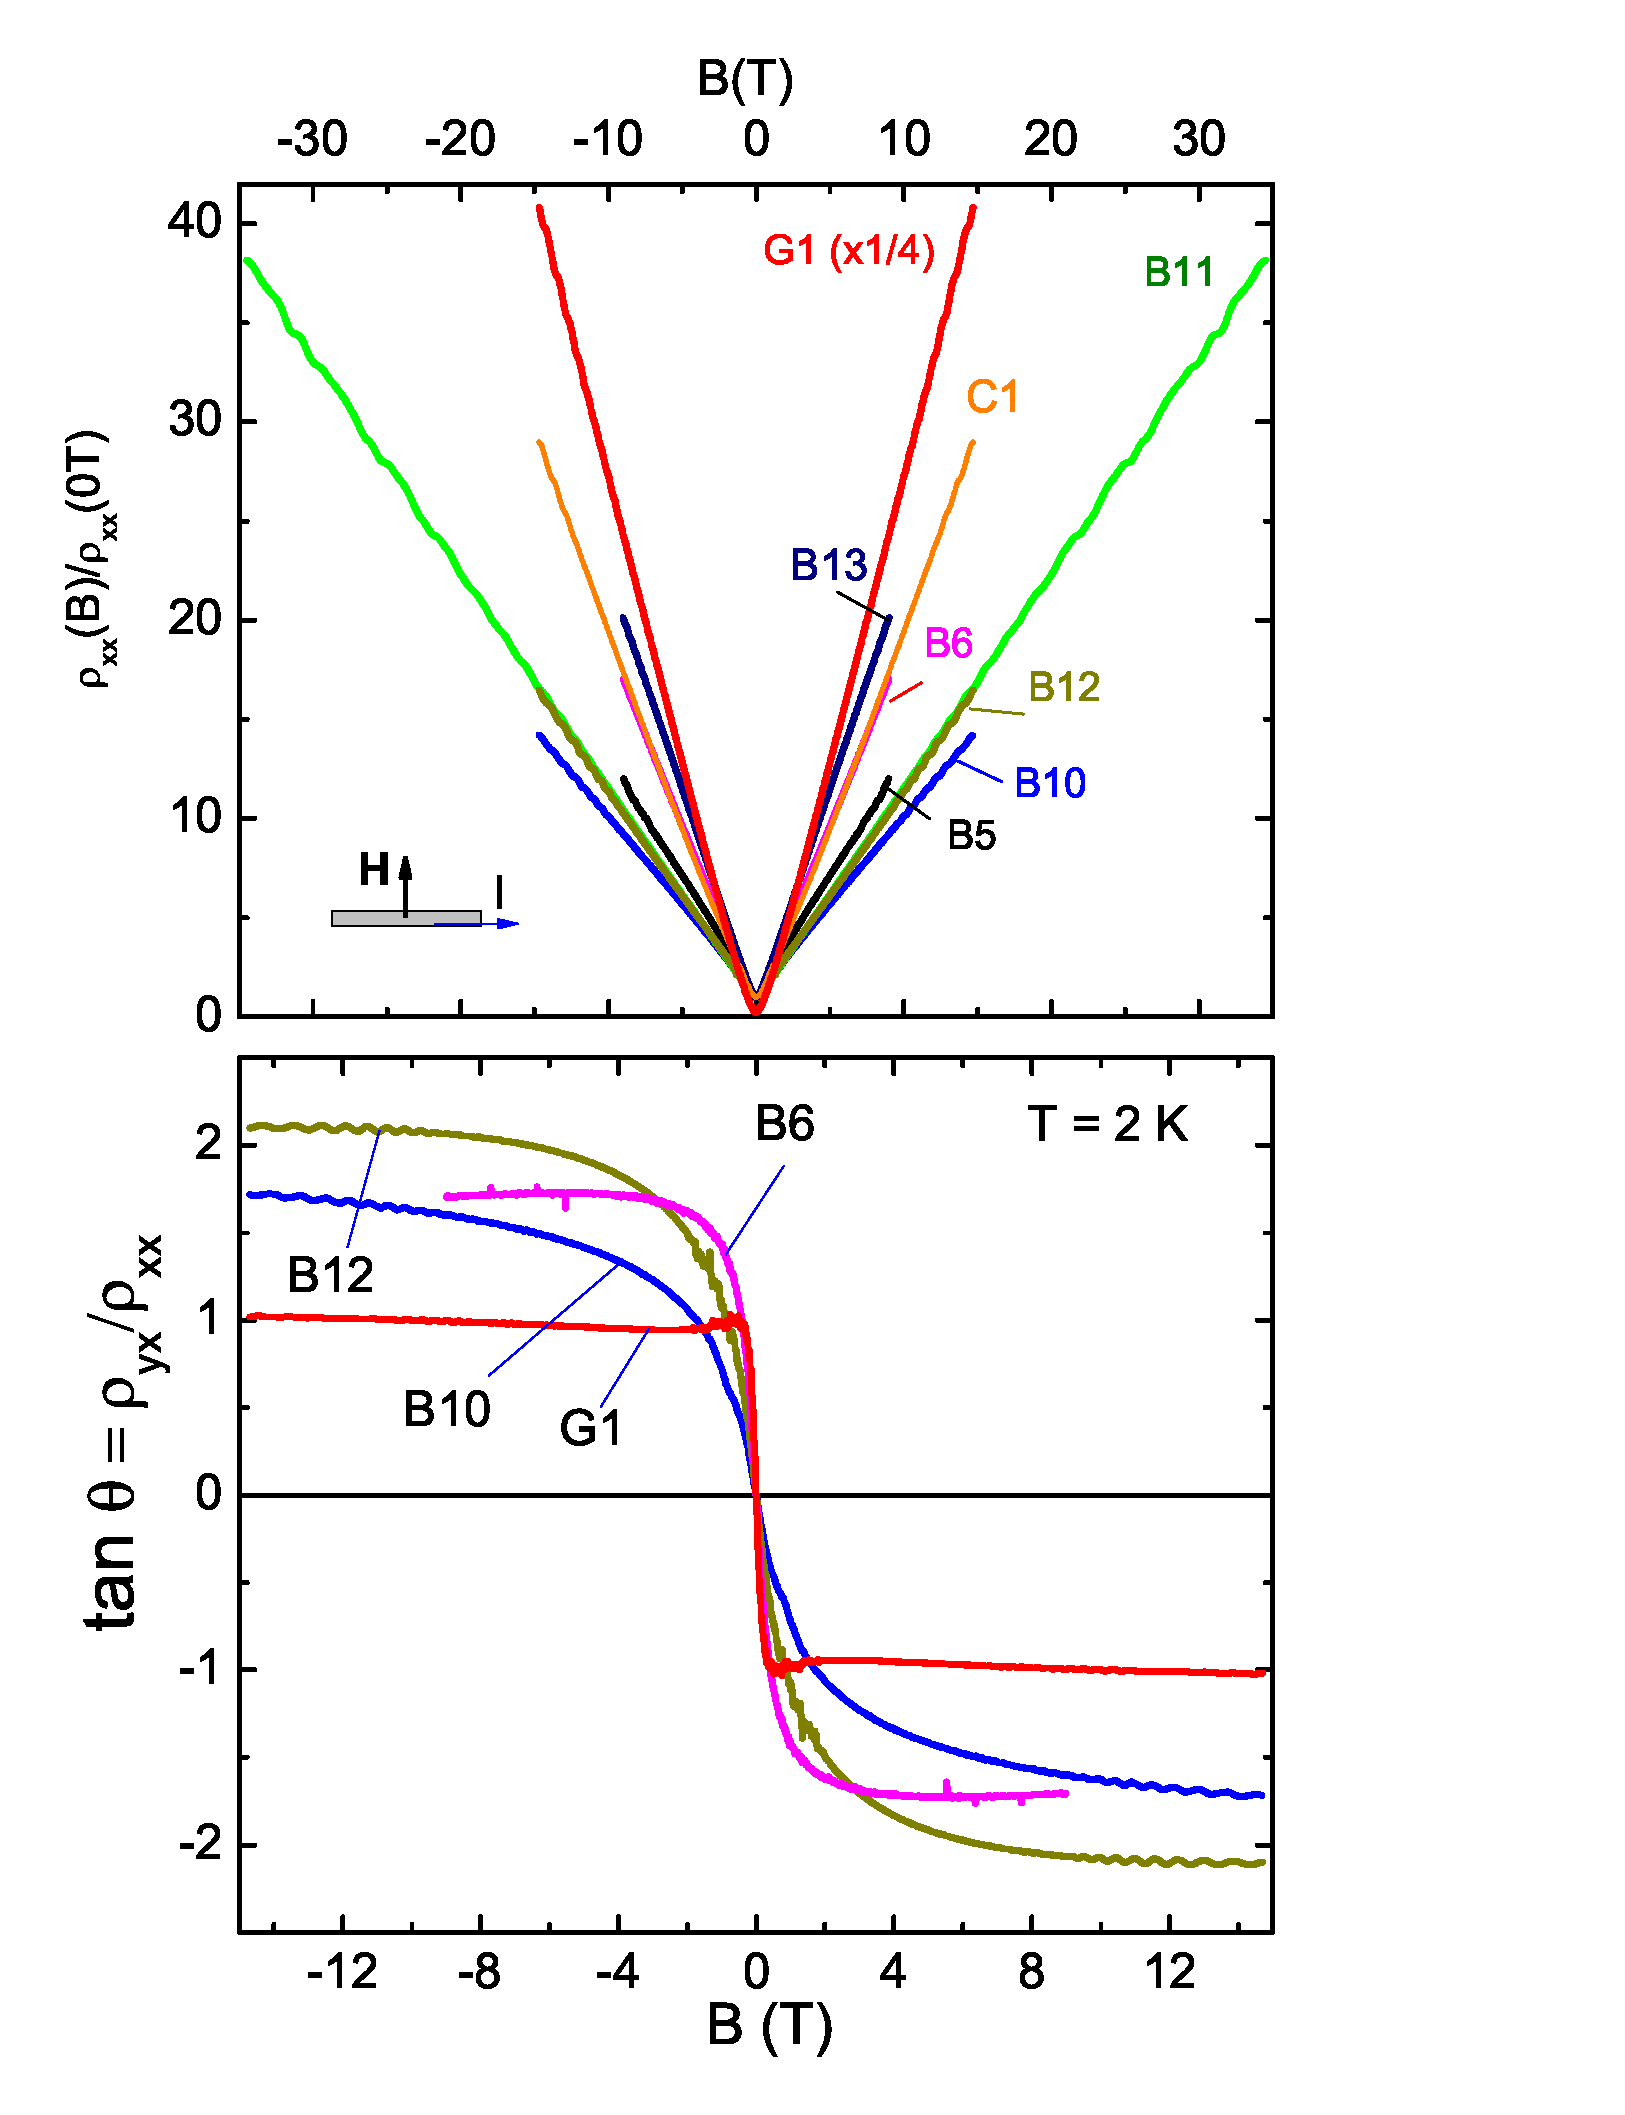
\includegraphics[width=0.9\linewidth]{ch-na3bi/figures/FigMRHallAngle}
\caption{\label{figMRtan}
Robust $H$-linear magnetoresistance in Na$_3$Bi (Panel A). In the 8 samples displayed here, $\rho_{xx}(B)$ is measured with $\bf H||\hat{c}$ at 2 K in all cases except in B11 (at 1.6 K). In B11, the MR persists without observable deviation to 35 T. A general trend is that the MR increases with $\mu$, from $\sim 14$ (at 15 T) in B10, to $\sim 160$ in G1 (which has the highest $\mu$) (the MR in G1 is plotted in $\frac14$ scale). In Panel B, the field profile of $\tan\theta = \rho_{yx}/\rho_{xx}$ is compared in 4 samples. As $H$ increases, $\tan\theta$ rapidly saturates to an $H$-independent value, which implies the anomalous relationship $\tau_{tr}\sim 1/H$. In G1, the change occurs at 0.5 T.}
  \end{center}
\end{figure}


To verify the above speculation on the same power law behavior of $\sigma_{xx}$ and $\sigma_{xy}$, we plot the $B$ dependences of $\sigma_{xx}$ and $\sigma_{xy}$ in log-log scale for the two high-mobility samples B6 and G1 (Fig. \ref{figCond}). The same slope of both of $\sigma_{xx}$ and $\sigma_{xy}$ in both samples indicates the same power-law dependence $B^{-\beta}$ at high fields. Compared with the starting field for the saturation of $\tan\theta$, we find that starting field of the same power-law dependence is also at $B$ = 2 T and 0.3 T in B6 and G1 respectively. This consistency provides a reasonable support for our explanation. We also notice that the measured value of $\beta$ is 1.0 in B6, but is slightly larger (1.15) in G1. 



%We will also compare the behavior of Na$_3$Bi and Cd$_3$As$_2$.





%%%%%%%%%%%%%%%%%%%%%%%%


%%%%%%%%%%%%%%%%%%%%%%%%%%%
%%%%%%%%%%%%%%%%%%%%%%%%%%%
%%%%%%%%%%%%%%%%%%%%%%%%%%%
%\vspace{3cm}
%
%\newpage

%%%%%%%%%%%%%%%%%%%%%%%%%%%%%%%%%%
%%%%%%%%%%%%%%%%%%%%%%%%%%%%%%%%%%
%%%%%%%%%%%%%%%%%%%%%%%%%%%%%%%%%% FIGURE 1




%%%%%%%%%%%%%%%%%%%%%%%%%%%%%%%%%%
%%%%%%%%%%%%%%%%%%%%%%%%%%%%%%%%%%
%%%%%%%%%%%%%%%%%%%%%%%%%%%%%%%%%% FIGURE 2

%%%%%%%%%%%%%%%%%%%%%%%%%%%%%%%%%



%%%%%%%%%%%%%%%%%%%%%%%%%%%%%%%%%%
%%%%%%%%%%%%%%%%%%%%%%%%%%%%%%%%%%
%%%%%%%%%%%%%%%%%%%%%%%%%%%%%%%%%% FIGURE 3

%%%%%%%%%%%%%%%%%%%%%%%%%%%%%%%%%%


%%%%%%%%%%%%%%%%%%%%%%%%%%%%%%%%%%
%%%%%%%%%%%%%%%%%%%%%%%%%%%%%%%%%%
%%%%%%%%%%%%%%%%%%%%%%%%%%%%%%%%%% FIGURE 4

%%%%%%%%%%%%%%%%%%%%%%%%%%%%%%%%%%


%%%%%%%%%%%%%%%%%%%%%%%%%%%%%%%%%%
%%%%%%%%%%%%%%%%%%%%%%%%%%%%%%%%%%
%%%%%%%%%%%%%%%%%%%%%%%%%%%%%%%%%% FIGURE 5

%%%%%%%%%%%%%%%%%%%%%%%%%%%%%%%%%%

%\newpage
\hfill \break

\begin{table*}[!htbp]
  \begin{center}
\begin{tabular}{|c|c|c|c|c|c|c|c|c|} \hline
Sample	& $\rho$(4 K)       & $n_H$	& $k_F$ &     $n_F$       &  $\mu'$    &     $\mu$  & MR(9 T)  & $\tau_{tr}$ \\ \hline
(units)   & $\;\;\mu\Omega$cm$\;\;$ & $10^{19}$ cm$^{-3}$  &  $\rm{\AA}^{-1}$    &   $10^{19}$ cm$^{-3}$      &  cm$^2$/Vs      & cm$^2$/Vs  & --  & ps \\ \hline\hline
B5		  &	34         &			  --      &	  0.083		 &  3.8      &     	--    &   --		         &    5.69   &   -- \\ \hline
B6		  &  6.2		        &   2.9		&   0.079		 &  	3.4     &		35,000    &   39,200    &  17     &   2.55 \\ \hline
B10	  &  7.5				   &  6.5				& 	0.081      &		3.6    &    13,000    &  	21,600  & 9.62   &  1.49  \\ \hline
B11	  &  87        &  1.3				&  0.073			&  	2.6 			&  5,500        &     --        &  10.5  &  --  \\ \hline
B12	  &  7.4        &  3.7				&  0.082			&  	3.7 			&  23,000        &  27,900  &    10.3 &  1.94 \\ \hline
C1			&  5.1					&  8.9				&  0.084			&   4.0			&  13,600      &   26,500    & 16.2  &  1.93  \\ \hline
F1	      &  6.6         &  6.5         &  0.082     &   3.7     &   14,600     &   30,400   &  32.8  &  2.11  \\  \hline
G1			&  1.72					&  4.6					&  0.085		&   4.1			&  78,900	   &   91,000   & 97.1   &   6.71 \\ \hline
\end{tabular}
\caption{\label{tab}
Transport parameters in 8 samples of Na$_3$Bi. $n_H$ is the Hall density inferred from $R_H$. $k_F$ is the FS wavevector inferred from the period of the quantum oscillations and $n_F = g_vk_F^3/3\pi^2$ with $g_v =2$. $\mu'$ is the transport mobility derived from $\rho$(4 K) and $n_F$, while $\mu$ is directly read from the profile of $\sigma_{xy}(B)$ in Fig. 3B (main text). MR(9 T) is the MR ratio measured at 9 T. $\tau_{tr}$ is calculated from $\mu = ev_F\tau_{tr}/\hbar k_F$. The quantities $\rho$, $n_H$ and $\mu$ are subject to the large uncertainty in estimating $t$ ($\pm 50\,\mu$m), but $k_F$, $n_F$ and $\mu_H$ are unaffected. F1 and G1 were post-annealed for 2 weeks and 1 month, respectively. The quantities $\rho$(4 K) and $n_H$ are strongly affected by the large uncertainty in $t$, but $k_F$, $n_F$, $\mu$ and $\tau_{tr}$ are not.
}
  \end{center}
\end{table*}




As described above, the observed transport properties of Na$_3$Bi are unexpected, and may need further and systematic theoretical study of the transport theory on Dirac semimetals. The Dirac semimetal may be regarded as the limiting case when TRI is present and the paired Weyl nodes coincide at the same point in $\bf k$ space, protected by the crystalline symmetry. As a result, the Berry curvature generated by different Weyl nodes annihilates. When TRI is broken in a magnetic field, the Berry curvature $\vec{\Omega}(\bf k)$ will appear and evolve as the B increases. Therefore, the FS topology may be changed in a magnetic field, and may lead to the unconventional behavior of  $\sigma_{xx}$ and $\rho_{xx}$ in transport experiments. But to completely understand this effect, there needs to be more specific theory that addresses the evolution of FS and scattering time in a high magnetic field.
%\newpage
\section{Evidence for Chiral Anomaly in Na$_3$Bi}
\label{sec:na3bi:chiral}

In this section, we discuss our evidence for the chiral anomaly effect in Na$_3$Bi. We will demonstrate the negative longitudinal magnetoresistance(LMR) data of two Na$_3$Bi samples, and compare them with the theoretical predictions. Besides, we will discuss the unexpected results obtained and their possible reasons. Also, to compare with the MR data of Na$_3$Bi, we will present the resistivity and conductivity tensors in a tilted $\bf B$ for a conventional one-band anisotropic metal. We will show why the conventional transport theory deviates from our observations. Additionally, we will calculate the splitting magnitudes of the Weyl nodes as we discussed in above sections. At the end, we explain why the negative MR in our Na$_3$Bi samples cannot arise from localization. All these evidences suggest the chiral anomaly origin of the negative LMR in our samples.


\subsection{Negative Longitudinal Magnetoresistance in Na$_3$Bi}

Besides the above type of Na$_3$Bi with a high carrier density, we have also grown some Na$_3$Bi crystals with a much lower Fermi energy $E_F$. The crystals were grown in a similar way as we described above, but were annealed for ten weeks before opening the growth tube. The samples are also contacted and sealed in a plastic cell inside the argon glovebox before being loaded into the magnet, as discussed in the chapter ``Experimental Setup''. As shown in Fig.\ref{figWeyl}B, C, the $\rho$ v.s. $T$ profile displays a non-metallic behavior and the Hall effect indicates a low $n$-type carrier density $n\sim 1\times 10^{17}$ cm$^{-3}$. The Fermi wavevector that corresponds to this carrier density is $k_F = 0.013 \;\rm{\AA}^{-1}$ ($8\times$ smaller than $k_D$). The saturation of resistivity below 10 K indicates the dominance of electrons in the conductance, and the mobility we obtain is $\mu\sim$ 2,600 cm$^2$/(Vs). Due to the zero gap feature of 3D Dirac semimetals, the holes in the valence band are copiously excited even at low $T$. As a result, the Hall coefficient $R_H$ shown in Fig. \ref{figWeyl}C is $n$-type at low temperatures but changes sign above 62K. We could also estimate $E_F$ using the maximum in $R_H$ at 105 K, and it yields a $E_F\sim 3k_BT\sim$ 30 meV. 
%The unusual profiles of $\rho$ and the Hall coefficient $R_H$ in Fig.\ref{figWeyl}C imply the zero-$B$ energy spectrum shown in Fig.\ref{figWeyl}B. 

\begin{figure}[!htbp]
  \begin{center}
\includegraphics[width=1\linewidth]{ch-na3bi/figures/FigWeylRhoHall.pdf}
\caption{\label{figWeyl} 
(Panel A) Sketch of the Landau levels in a Weyl semimetal showing chiral states in the lowest LL with opposite velocities and chiralities (arrows)
$\parallel\bf B$. An $\bf E$-field $\parallel \bf B$ breaks chiral symmetry and leads to an axial current. 
Panel B shows the Fermi energy $\epsilon_F$ and the density of states $D(\varepsilon)$ in zero $B$ (bold curve). 
$f(\varepsilon)$ is the Fermi-Dirac distribution at 3 K and at $\sim$100 K. The inset shows the triangle anomaly that dictates the decay of the neutral pion $\pi^0$ into 2 photons $\gamma$. 
(Panel C) The $T$ dependence of the resistivity $\rho$ in $B=0$ and Hall coefficient $R_H$ in Na$_3$Bi.
$R_H$ is measured in $B<$2 T applied $\parallel \bf c$. At 3 K, $R_H$ corresponds to a density $n = 1.04\times 10^{17}$ cm$^{-3}$.  
The excitation of holes in the valence band leads to a sign change in $R_H$ near 70 K and a steep decrease in $\rho$. The inset shows the contact labels and the $x$ and $y$ axes fixed to the sample. 
(Panel D) Curves of the longitudinal magnetoresistance $\rho_{xx}(B,T)$ at selected $T$ from 4.5 to 300 K measured with $\bf B\parallel \hat{x}$ and $I$ applied to (1,4). The steep decrease in $\rho_{xx}(B,T)$ at 4.5 K reflects the onset of the axial current in the lowest LL. As $T$ increases, the occupation of higher LLs in conduction and valence bands overwhelms the anomalous term.
}
  \end{center}
\end{figure}

Analysis of the observed Shubnikov de Haas (SdH) oscillations (see below) in magnetoresistance also confirms the value of $E_F$ in our Na$_3$Bi samples. Fig. \ref{figSdH}A displays the clear SdH oscillations with a small frequency (a smooth background has been subtracted from the raw data) when $\bf B$ is aligned towards $\bf c$ . Through locating the index field $B_n$ as the extrema of the SdH oscillations, we obtain the Landau index plot in Fig.\ref{figSdH}B. A linear fitting to the index plot yields a FS cross section $S_F$= 4.8$\pm$ 0.3 T, corresponding to $E_F = 29\pm 2$ mV which is in a good agreement with the value from $R_H$. The SdH period also implies that $E_F$ enters the $N$ = 0 LL at $B$ = 6-8 T. 





The density inferred from $S_F$ ($n_e = 1.4\times 10^{17}$ cm$^{-3}$) is slightly higher than $n_H$. We also notice that there is some deviation from the straight line in Fig. \ref{figSdH}B, which may be explained by a $g$-factor of $\sim$20, comparable to that in Cd$_3$As$_2$observed~\cite{Jeon2014} by scanning tunneling microcsopy ($g^*\sim$ 40). Such a low $E_F$ suggests that the transport property of the 3D Dirac fermions in Na$_3$Bi crystals can be influenced more significantly by the splitting of Weyl nodes and the resulted charge pumping effect between the nodes. Therefore, this type of Na$_3$Bi crystals provides us a great opportunity to investigate the chiral anomaly effect predicted for Weyl fermions.


\begin{figure}[!htbp]
  \begin{center}
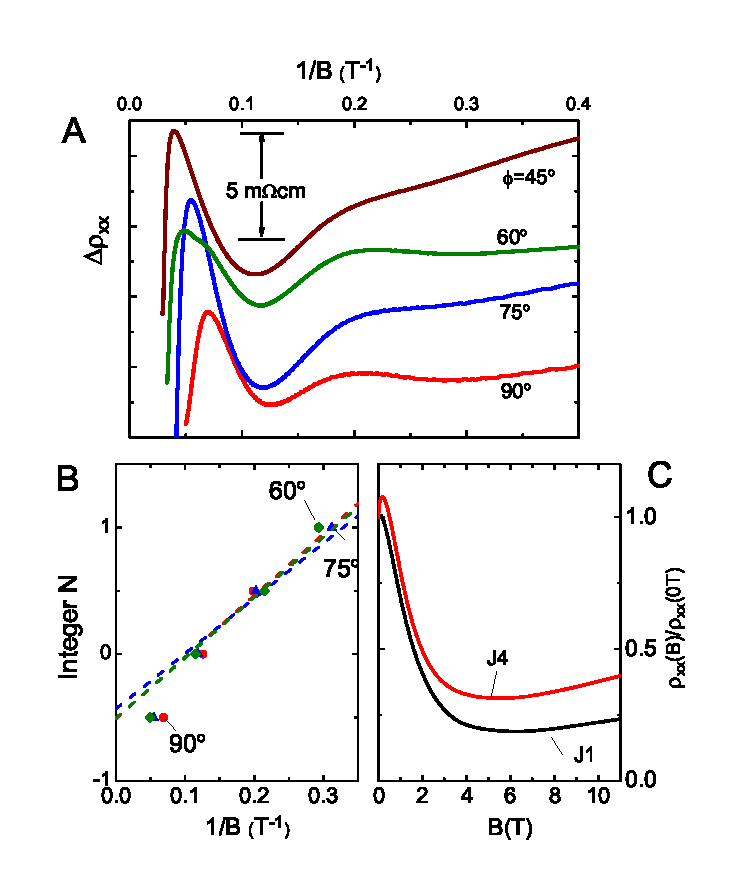
\includegraphics[width=0.9\linewidth]{ch-na3bi/figures/FigSdHMR}
\caption{\label{figSdH}
Panel A shows the Shubnikov oscillations resolved in $\rho_{xx}$ for several tilt angles $\theta$ (relative to $\bf \hat{x}$) after subtraction of the positive $B$-linear MR background (vertical scale as shown). The slope of the plot of the Landau level index $N$ vs. $1/B_n$ where $B_n$ locates the extrema of the oscillations yields $S_F$ = 4.8$\pm$ 0.3 T, $k_F$ = 0.013 $\rm{\AA}^{-1}$, and $E_F$ = 29$\pm$2 mV.  The deviation at large $B$ is consistent with a large $g^*\; (\sim 20)$. The field profiles of of $\rho_{xx}$ (inferred from $R_{14,23}$) in Sample J1 and J4, with $\bf B\parallel I$. The $N =0$ LL is entered at $B$= 6-8 T. The slight increase for $B>$ 5 T reflects the narrow width of the axial current. A slight misalignment of $\bf B$ (the uncertainty here is $\pm 1^\circ$) allows the $B$-linear positive MR component to appear as a background at large $B$. 
}
  \end{center}
\end{figure}


The 3D Dirac semimetals, Na$_3$Bi and Cd$_3$As$_2$~\cite{Wang2012,Wang2013}, comprise two Dirac cones located at opposite positions in the Brillouin Zone (Fig. \ref{figWeyl}A). Ref.~\cite{Wang2012} has provided detailed calculations to show that each Dirac cone could be separated into both left- and right-handed (Weyl) states that do not mix~\cite{Burkov2011,Yang2011, Aji2012,Son2013,Parameswaran2014,Hosur2013} when the time-reversal symmetry (TRS) is broken by the magnetic field. Besides, an axial current that flows between the paired Weyl nodes could be induced while both $\bf E$ and $\bf B$ are present, and it results in the negative longitudinal magnetoresistance in the semiclassical region as Son et.al.~\cite{Son2013} point out. Triggered by the above predictions, many experimental groups recently reported their negative MR results in different semimetals, such as  Bi$_{1-x}$Sb$_x$~\cite{Kim2013}, Cd$_3$As$_2$~\cite{Liang2015,Zhang2015a}, ZrTe$_5$~\cite{Li2014} and TaAs~\cite{Zhang2015}. However, we need to be cautious before reaching any conclusion because such negative MR exists in semimetals that are not Dirac or Weyl materials (e.g. Cd$_x$Hg$_{1-x}$Te~\cite{HgTe} and PdCoO$_2$~\cite{Kikugawa2014}). Thus it is important to identify a unique feature that could only be explained by the charge pumping effect and distinguishes the chiral anomaly from other effects in crystals. Below we will discuss a unique negative MR signature in Na$_3$Bi. We find that the enhanced conductance has a narrow plume shape whose direction is locked to the direction of $\bf B$. The enhancement steered by $\bf B$ suggests that it originates from the $\bf E\cdot \bf B$ pumping term.




%The intriguing possibility of observing the chiral (or axial) anomaly as a novel charge current in a crystal has been discussed since 1983~\cite{Nielsen}. In the field of topological phases of matter, this question has lately received intense interest in the context of Weyl semimetals~\cite{Ashvin,Balents,Son,Sid,Hosur}. [The anomaly first appeared as the dominant channel for the decay of the neutral pion into 2 photons $\pi^0\to 2\gamma$ (the Adler-Bell-Jackiw anomaly~\cite{Adler,Bell}). Subsequently, it has served broadly as a no-go test for the renormalizability of chiral gauge theories~\cite{Peskin,Zee}.]  To realize a Weyl semimetal, a promising path is to start with a 3D Dirac semimetal~\cite{Young,Bernevig}, and then split each Dirac node into a pair of Weyl nodes using a magnetic field $\bf B$. Rapid progress in identifying candidates for Dirac semimetals has been made~\cite{Young,Bernevig,Wang1,Wang2,Nagaosa}. The two semimetals specifically identified~\cite{Wang1,Wang2}, Na$_3$Bi and Cd$_3$As$_2$, were recently confirmed to be so by angle-resolved photoemission (ARPES)~\cite{Chen,Borisenko,Neupane,Liu,Suyang} and scanning tunneling microscopy~\cite{Yazdani}. Here we report the detection of the axial current in Na$_3$Bi as a highly collimated beam locked to the direction of $\bf B$.

A magnetic field $\bf B$ could split each Dirac node into two Weyl nodes with opposite chiralities $\chi=\pm 1$~\cite{Hosur2013,Wang2012} respectively. These Weyl nodes may be regarded as monopole sources and sinks of Berry curvature in $\bf k$ space. The Landau levels formed by these states are shown in Fig. \ref{figWeyl}B. One important feature in the LLs is that the lowest LL has a strict linear dispersion. And the chirality, which describes the handedness of the fermions, will determine whether the velocity is directed to the left or to the right. Therefore, it provides a solid-state platform to study the charge-pumping effect between fermions with different chiralities. In the absence of an electric field $\bf E$, the two chiral populations are separately conserved (Fig. \ref{figWeyl}A). However, application of $\bf E$ ruins the conservation and leads to a charge-pumping process between nodes, corresponding to the chiral anomaly sketched in Fig. \ref{figWeyl}B~\cite{Nielsen1983,Wan2011,Burkov2011,Son2013,Parameswaran2014,Hosur2013}. In a combination of $\bf E$ and $\bf B$, the electrons' charge-pumping rate between the two chiral branches is
\be
W = \chi\frac{e^3}{4\pi^2\hbar^2} {\bf E\cdot B},
\label{eq:W}
\ee
which is the direct result of the chiral anomaly effect~\cite{Burkov2011,Yang2011, Aji2012,Son2013,Parameswaran2014,Hosur2013}. When $\bf E$ and $\bf B$ are parallel, the pumping rate reaches the maximum, while the rate vanishes when $\bf E \perp \bf B$. Ideally, such pumping effect generates a longitudinal (axial) current. However, different from high energy physics, the charge pumping effect in a crystal is relaxed by the intervalley scattering. A relaxation time approximation describes the scattering rate as $1/\tau_v = CeB/\hbar v$, i.e. proportional to the LL degeneracy~\cite{Aji2012}. As a result, in the quantum limit, although the pumping rate becomes larger as the $B$ increases, the increment of the scattering rate counteracts that of the pumping rate. Thus the conductivity $\sigma_\chi\sim W\tau_v$ becomes independent of $B$ in the quantum limit. When many LLs are occupied, the axial current remains observable although reduced. In the semiclassical weak-$B$ limit, Son and Spivak~\cite{Son2013} show that
\be
\sigma_{\chi} = \frac{e^2}{4\pi^2\hbar c}\frac{v}{c}\frac{(eBv)^2}{E_F^2}\tau_v.
\label{eq:SS}
\ee
In contrast to the quantum limit case, the field dependence of $\sigma_\chi$ follows a quadratic behavior instead of a constant. Hence, the whole field picture of $\sigma_\chi$ has a $B^2$ growth at weak fields and a $B$-independent saturation in the quantum limit.

%%%%%%%%%%%
%As mentioned, the breaking of the time-reversal symmetry (TRS) by $\bf B$ causes each Dirac node to split into two Weyl nodes~\cite{Fang2012,Wang2012,Wang2013}. The Weyl nodes, which may be regarded as monopole sources and sinks of Berry curvature in $\bf k$ space, come in pairs with opposite chiralities $\chi=\pm 1$. In the absence of an electric field $\bf E$, the two chiral populations are separately conserved (Fig. \ref{figWeyl}A). However, application of $\bf E$ ruins the conservation and leads to a charge-pumping process between nodes, corresponding to the chiral anomaly sketched in Fig. \ref{figWeyl}B~\cite{Nielsen1983,Wan2011,Burkov2011,Son2013,Parameswaran2014,Hosur2013}. As shown in Fig. \ref{figWeyl}A, the lowest Landau level (LL) of the Weyl states in a crystal is chiral. For $\chi = 1$ the lowest LL is right-moving (velocity $\bf v\parallel \bf {B}$), whereas for $\chi=-1$ it is left-moving~\cite{Nielsen1983,Wan2011,Burkov2011,Son2013,Hosur2013}. At steady state, $\bf E$ transfers charge from say the $\chi = -1$ branch to the $\chi= 1$ branch at the rate below:~\cite{Hosur2013}
%\be
%W = \chi\frac{e^3}{4\pi^2\hbar^2} {\bf E\cdot B}.
%\label{eq:W}
%\ee
%The rate peaks for $\bf E\parallel B$ and vanishes when $\bf E\perp B$. In the weak-$B$ limit, a Berry curvature approach gives the chiral conductivity~\cite{Son2013} 
%\be
%\sigma_{\chi} = \frac{e^2}{4\pi^2\hbar c}\frac{v}{c}\frac{(eBv)^2}{\epsilon_F^2}\tau_v,
%\label{eq:SS}
%\ee
%where $\tau_v$ is the intervalley life-time and $\epsilon_F$ the Fermi energy. 

%The Dirac semimetal Na$_3$Bi grows as mm-sized, deep-purple, plate-like crystals with the largest face parallel to the $a$-$b$ plane ($\bf \hat{c}$ is normal to the planes). We annealed the crystals for 10 weeks before opening the growth tube~\cite{Satya}. To avoid oxidation, crystals were contacted using silver epoxy  in an Argon glove box, and then immersed in paratone in a capsule before rapid cooling. In Na$_3$Bi, the Dirac nodes are located at the wave vectors $(0,0, \pm k_D)$ with $k_D \simeq 0.1\; \mathrm{\AA}^{-1}$~\cite{Chen,Suyang}. The predicted existence of surface Fermi arcs was recently confirmed~\cite{HasanFS}. Initial experiments in our lab~\cite{Xiong} on samples with a large Fermi energy $\epsilon_F$ (400 mV) showed only a positive MR with the anomalous $B$-linear profile reported in Cd$_3$As$_2$~\cite{Liang}. 
%
%
%In a field $\bf B||\hat{z}$, each Dirac node divides into two Weyl nodes of chirality $\chi=\pm 1$~\cite{Hosur,Wang1}. As shown in Fig. \ref{figWeyl}B, the states are quantized into LLs. Specific to Weyl states, however, the lowest LL ($N$=0) has a constant slope, with velocity directed either to the left or to the right, depending on $\chi$. This dichotomy is the crystal analog of the left and right-handed populations~\cite{Nielsen}. Application of $\bf E\parallel \bf B$ leads to charge-pumping of electrons between the two branches at the rate
%\be
%W = \chi\frac{e^3}{4\pi^2\hbar^2} {\bf E\cdot B},
%\label{eq:W}
%\ee
%which expresses the chiral anomaly~\cite{Nielsen,Ashvin,Balents,Ran,Aji,Son,Sid,Hosur}. In the presence of impurities, the longitudinal (axial) current relaxes via an intervalley scattering rate given by $1/\tau_v = CeB/\hbar v$, i.e. proportional to the LL degeneracy~\cite{Aji}. Hence, the chiral conductivity $\sigma_\chi\sim W\tau_v$ is independent of $B$ in the quantum limit. We emphasize that, when many LLs are occupied, the axial current remains observable although reduced. In the weak-$B$ limit and when $\bf E$ and $\bf B$ are parallel, Son and Spivak~\cite{Son} show that
%\be
%\sigma_{\chi} = \frac{e^2}{4\pi^2\hbar c}\frac{v}{c}\frac{(eBv)^2}{E_F^2}\tau_v.
%\label{eq:SS}
%\ee
%As $B$ increases, $\sigma_\chi$ grows as $B^2$, but saturates to a $B$-independent value in the quantum limit.



We have seen such a B dependence in the longitudinal magnetoresistance of our Na$_3$Bi samples when $\bf B\parallel\hat{x}\parallel E $. As shown in Fig. \ref{figWeyl}D, the resistivity $\rho_{xx}$ displays a large negative LMR ($\bf B\parallel\hat{x}\parallel I $, the current) at low temperatures. The resistance measured is $R_{14,23}$ (defined in Fig. \ref{figWeyl}C, inset and caption). $\rho_{xx}$ has a peak around $B=0$ T, and then has a sharp decrease until it becomes nearly field independent at higher fields. The peak is suppressed as $T$ increases above $\sim$100 K (Fig. {figWeyl}D). In Fig. \ref{figSdH}C, the saturation of $\rho_{xx}$ (in Sample J1 and J4) happens above 5 T (the slight upturn at higher fields is a hint that the axial current is sensitive to misalignment of $\bf B$ at the level $\pm 1^{\circ}$). It is unexpected to see such a large negative LMR in a conventional conductor, even with band anisotropy (see below).

Then we hope to test whether this anomalous negative LMR arises from the chiral anomaly effect. Since the charge pumping rate is determined by the $\bf E\cdot \bf B$ term, it reaches the maximum when $\bf B$ is aligned with $\bf E$. We notice that the pumping rate only depends on the relative direction of $\bf E$ and $\bf B$ and does not care about the physical direction of them, when the field strengths are fixed. Thus a crucial test then is the demonstration that, the negative magnetoresistance (MR) pattern remains the same if $\bf E$ is rotated by 90$^\circ$. If it does, the axial current maximum is meant to be locked to $\bf B$ and $\bf E$, rather than being pinned to the crystal axes, even for weak $B$. Besides, we also need to test whether the axial current becomes smaller when $\bf B$ deviates from the direction of $\bf E$ with $\bf E$ fixed.

\begin{figure}[!htbp]
  \begin{center}
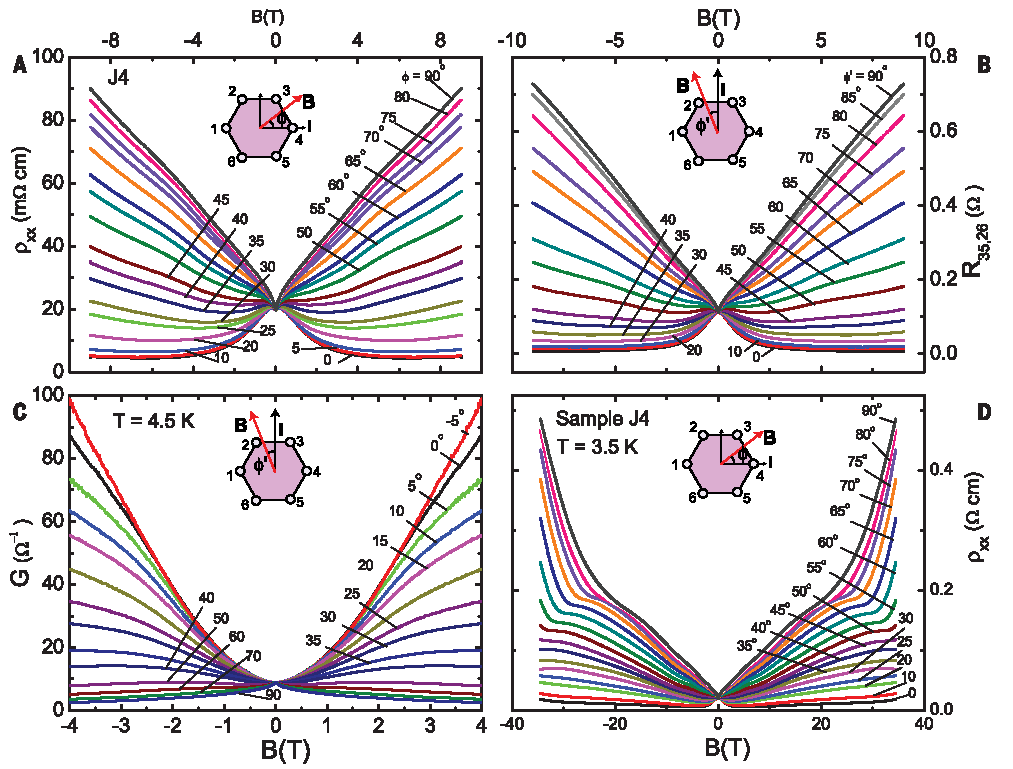
\includegraphics[width=1\linewidth]{ch-na3bi/figures/FigMR4.pdf}
\caption{\label{figMR4}
Evidence for axial current in Na$_3$Bi (J4) obtained from transport measurements in an in-plane field $\bf B$. Panel A shows plots of the resistivity $\rho_{xx}$ vs. $B$ at selected field angles $\phi$ to the $x$-axis (inferred from resistance $R_{14,23}$, see inset). For $\phi$ = 90$^\circ$, $\rho_{xx}$ displays a $B$-linear positive MR. However, as $\phi\to 0^\circ$ ($\bf B||\hat{x}$), $\rho_{xx}$ is strongly suppressed. Panel B shows plots of $R_{35,26}$ with $\bf E$ rotated by 90$^\circ$ relative to Panel A ($\bf B$ makes angle $\phi'$ relative to $\bf\hat{y}$; see inset). The resistance $R_{35,26}$ changes from a positive MR to negative as $\phi'\to 0^\circ$. In both configurations, the negative MR appears only when $\bf B$ is aligned with $\bf E$. Panel C shows the conductance $G\equiv 1/R_{35,26}$. In weak $B$, it has the $B^2$ form predicted in Eq. \ref{eq:SS}~\cite{Son2013}. A fit to the parabolic form gives $\tau_v/\tau_{tr}$ = 40-60. Panel D shows curves of $\rho_{xx}$ (as in Panel A) extended to 35 T. Above 23 T, a knee-like kink appears at $H_k$. Above $H_k$, $\rho_{xx}$ increases very steeply (for $\phi >35^\circ$).}
  \end{center}
\end{figure}


Therefore, to carry out these tests, we first rotate $\bf B$ in the $x$-$y$ plane while still monitoring the resistance $R_{14,23}$ ($\bf E$ fixed to $\bf\hat{x}$ axis). Figure \ref{figMR4}A shows the $\rho_{xx}$ v.s. $B$ curves up to 9 T of Sample J4 measured at 4.5 K at selected $\phi$ (the angle between $\bf B$ and $\bf\hat{x}$). When $\phi = 90^\circ$ ($\bf B||\hat{y}$), the MR has an almost $B$-linear and positive shape as we observed in Cd$_3$As$_2$~\cite{Liang2015} and Na$_3$Bi~\cite{Xiong2015a} (as we discussed in previous sections ) with $\bf B||c$. As $\bf B$ rotates towards $\bf \hat{x}$ ($\phi$ decreased), the MR curves are pulled down towards negative values. When $\bf B$ and $\bf E$ are aligned ($\phi = 0$), the longitudinal MR has a rapid decrease and becomes fully negative (see below for the unsymmetrized curves, and results from Sample J1). 




%%%%%%%%%%%%%%%%%%%%%%%%%%%%%%%%%%
%%%%%%%%%%%%%%%%%%%%%%%%%%%%%%%%%%
%%%%%%%%%%%%%%%%%%%%%%%%%%%%%%%%%% FIGURE 



To rotate $\bf E$, we then made the MR measurement \emph{in situ} with $I$ applied to the contacts (3, 5). Thus $\bf E$ is rotated by 90$^\circ$ (the measured resistance is $R_{35,26}$). Remarkably, the observed MR pattern is also rotated by 90$^\circ$, even when $B<$ 1 T. We define the angle of $\bf B$ relative to $\bf\hat{y}$ as $\phi'$, and then find that the MR curves at selected $\phi'$ (Fig. \ref{figMR4}A) have a similar behavior to those at various $\phi$. The LMR also becomes fully negative when $\phi'$ reaches 0. The curves in Panels A and B are nominally similar, except that $\phi$ and $\phi'$ describe different directions of $\bf B$ and $\bf E$, and $\phi = 0$ and $\phi'=0$ refer to $\bf\hat{x}$ and $\bf\hat{y}$, respectively. As we discuss below, it is novel to see a negative MR pattern locked to the direction the common direction of $\bf E\parallel B$, regardless of the $\bf E$ direction relative to the crystal structure. We identify it as a signature of the chiral anomaly.


A surprise to us in the field-rotation experiment is the acute sensitivity of the axial current to any small angle between $\bf B$ and $\bf E$ at large $B$, as hinted at in Fig. \ref{figSdH}C and Fig. \ref{figMR4}. The slight misalignment of tiny degrees lead to the upcoming MR at high fields caused by scattering. To determine the angular dependence of $\sigma_\chi$, we measured $R_{14,23}$ at continuously tilted angles at a fixed $B$ with $\bf B$ tilting either in the $x$-$y$ or the $x$-$z$ plane. Figures \ref{figPolar4}A and \ref{figPolar4}B display the curves of $\Delta\sigma_{xx}(B,\phi) \equiv \sigma_{xx}(B,\phi)- \sigma_{xx}(B,90^\circ)$ vs. $\phi$ ($\bf B$ in the $x$-$y$ plane at angle $\phi$ to $\bf\hat{x}$), when $B$ is fixed at various fields from 0.5$\to$2 T (Panel A) and 3$\to$7 T (B) respectively. Panels C and D show the similar measurements except that $\bf B$ is in the $x$-$z$ plane at an angle $\theta$ to $\bf\hat{x}$. 

Interestingly, we find that angle dependence of $\Delta\sigma_{xx}$ at low fields has slightly sharper behavior than $\cos \phi$ (or $\cos \theta$). As displayed by the dashed curves in Fig. \ref{figPolar4}C and D, we could use a curve of $\cos^p\phi$ (or $\cos^p\theta$) with $p$ = 4 to reach a reasonably good fitting to the observed low-field angular dependence. Nevertheless, when $B$ grows larger than 2 T, the angular widths of $\Delta\sigma_{xx}$ become significantly narrower. Such a sharp dependence is unexpected. It also indicates that, at large $B$, the axial current is observed as a strongly collimated beam in the direction selected by $\bf B$ and $\bf E$ as $\phi$ or $\theta$ is varied. We notice that current theoretical works that have considered the MR modulation caused by the chiral anomaly effect, such as Ref. ~\cite{Son2013}, have only studied the case when $\bf B$ and $\bf E$ are parallel. A complete investigation of the MR enhancement at various angles is lacked. Also, due to the existence of the scattering term, $\Delta\sigma_{xx}$ may not simply follow the $\bf E\cdot \bf B$ term that describes the driven axial current. Since the strong collimation is unpredicted to our knowledge, we hope this experimental work can lead to more exploration on the conductivity enhancement caused by the chiral anomaly effect when $\bf B$ and $\bf E$ are not parallel.

\begin{figure}[!htbp]
  \begin{center}
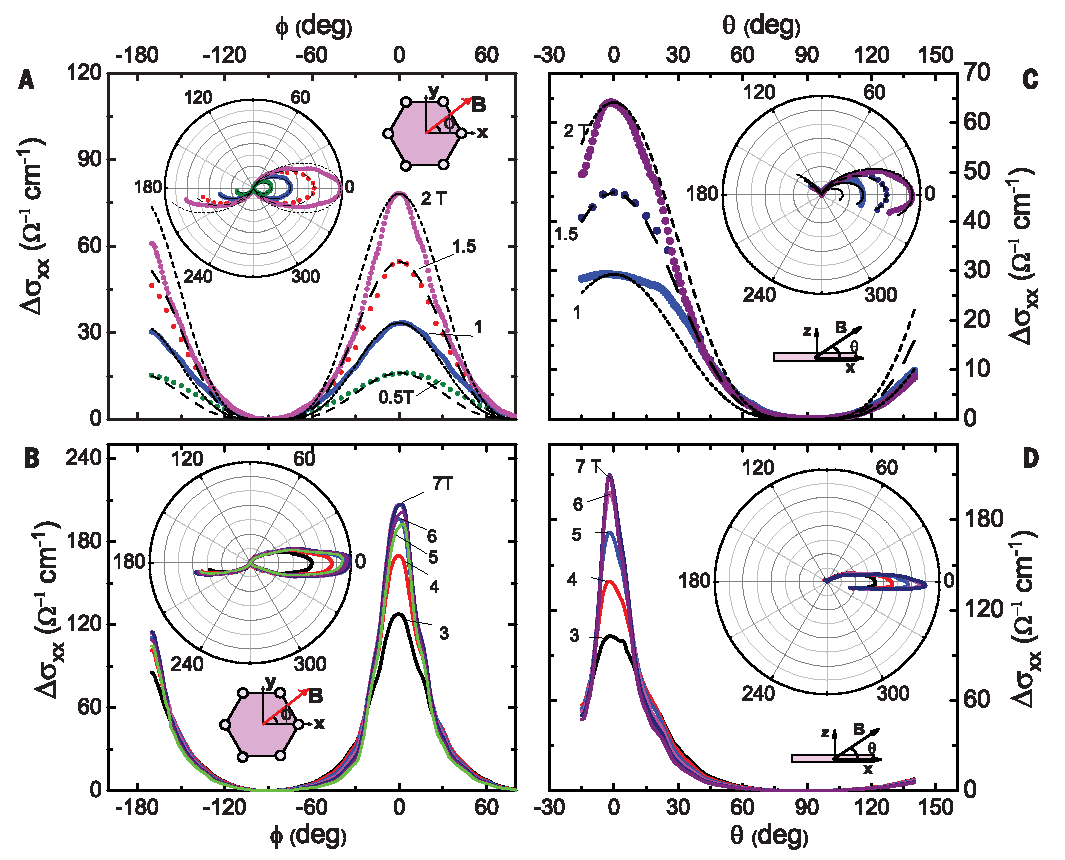
\includegraphics[width=1\linewidth]{ch-na3bi/figures/FigPolar4.pdf}
\caption{\label{figPolar4} 
Angular dependence of the axial current in Sample J4 at 4.5 K inferred from measurements of $R_{14,23}$ in tilted ${\bf B}(\theta,\phi)$. 
In Panels A and B, $\bf B$ lies in the $x$-$y$ plane at an angle $\phi$ to $\bf\hat{x}$ (sketch in insets). The 
conductance enhancement $\Delta \sigma_{xx}$ at fixed $B$ is plotted against $\phi$ for values of $B \le$ 2 T (Panel A) and for $3\le B\le 7$ T (Panel B). Fits to $\cos^4\phi$ (dashed curves), while reasonable below 2 T become very poor as $B$ exceeds 2 T. The insets show the polar representation of $\Delta \sigma_{xx}$ vs. $\phi$. In Panels C and D, $\bf B$ is tilted in the plane $x$-$z$. As sketched in the insets, $\theta$ is the angle between $\bf B$ and $\bf\hat{x}$. Curves of $\Delta \sigma_{xx}$ vs. $\theta$ for $B$ = 1, 1.5 and 2 T are shown in Panel C, while Panel D shows curves for $3\le B\le 7$ T. The axial current is peaked when $\phi\to 0$ (or $\theta\to 0$) with an angular width that narrows significantly as $B$ increases.
}
  \end{center}
\end{figure}

Another interesting part is that the negative MR is very large (as shown in Fig.\ref{figMR4}), which indicates a possible long relaxation time $\tau_a$. It is convenient to analyze the contribution of the axial current in conductance. We convert the resistivity into conductance in Fig. \ref{figMR4}C. When $\bf B$ and $\bf E$ are parallel, $G = 1/R_{35,26}$ follows a parabolic behavior that increases with $B$. The dramatic increase of $G$ indicates a long inter-valley relaxation time for the novel current. We fit Eq. \ref{eq:SS} to the $G$ v.s. $B$ curve at $\phi'=0$ in Fig. \ref{figMR4}C. Using the ratio $\sigma_{\chi}/\sigma_0 = \frac34 (k_F\ell_B)^{-4}.(\tau_v/\tau_{tr})$, where $\sigma_0$ is the Drude conductivity, $\ell_B$ is the magnetic length $\sqrt{\hbar/eB}$ and $\tau_{tr}$ the usual transport lifetime, we find that $\tau_v/\tau_{tr}$ = 40-60 in weak $B$. Such a large ratio between the two types of relaxation time implies that the inter valley relaxation rate $1/\tau_v$ of the novel axial current is anomalously lower than the scattering rate $1/\tau_{tr}$ of the conventional states in zero $B$. However, in the quantum limit, $\tau_v$ is strongly suppressed as $\sim 1/B$ because of the continuous increment in LL degeneracy which makes $\sigma_\chi$ $B$-independent, as discussed above (Fig. \ref{figSdH}C). 

To our knowledge, the matrix element $M$ in $1/\tau_a$ is not well studied despite its importance. Thus our data on Na$_3$Bi can provide a helpful direction for the study of the relaxation process of axial currents. Besides, there is some debate on whether a large node separation $2\delta k_N$ is needed to obtain a long $\tau_a$. In a DSM such as Na$_3$Bi, the Weyl nodes originally occupy the same point in the reciprocal space. But they can be split by a magnetic field. We deduce the separation induced by $\bf B$ in our Na$_3$Bi samples using the estimate of $g^* \sim 20$. We find that $\delta k_N > k_F$ when $B > 12$ T. Interestingly, it was shown\cite{Burkov2015} recently that the ratio $\tau_a/\tau_0$ (in a superlattice model) can be very large even for negligible $\delta k_N$. Ref. \cite{Burkov2015} argues that the axial current relaxation is still hampered by the Berry curvature effects while the chiral symmetry is only weakly violated. This issue should be resolvable by future LMR experiments.

%Then we hope to estimate splitting speed of the Weyl nodes of a DSM in a magnetic field. This information is important because the charge pumping effect in a DSM is based on the prediction that Weyl nodes splitting is generated by breaking time reversal symmetry in the DSM. And the displacement of the Weyl node $\delta K$ from the Dirac node in a DSM is governed by $\delta K= \pm g^*\mu_B B/(\hbar v)$ (we will explain the details later). Assuming $g^*\sim50$ (roughly that in Cd$_3$As$_2$~\cite{Jeon2014}) and $v\sim 2\times 10^5$ m/s, we estimate that the Weyl spheres separate ($\delta K > k_F$) when $B>$ 6 T. This significant displacement is consistent with the steep increase in $\sigma_\chi$ in modest $B$.  




We also notice some interesting features in the high field part of $R_{14,23}$ up to $B$ = 35 T. As displayed in Fig. \ref{figMR4}D, at $H_{k}\sim$ 23 T when $\bf B||\hat{y}$, the slopes of the MR curves experience a sudden change. As $\bf B$ is tilted away from $\bf\hat{y}$ ($\phi\to \; 55^\circ$), the feature at $H_k$ becomes better resolved as a kink. The steep increase in $\rho_{xx}$ above $H_k$ may suggest an electronic instability at large $B$ that opens an energy gap. We also notice that $H_k(\phi)$ is sensitive to the angle $\phi$ as the decrease in $\phi$ below $45^\circ$ rapidly increases $H_k(\phi)$ to above 35 T. However, the negative MR curves close to $\phi = 0$ remain almost unaffected by the instability up to 35 T (the small rising background is from a weak $B_z$ due to a slight misalignment and implies the strong collimation of the axial current). 

The above experimental observation can not be explained by the conventional transport theory, and in our view, provides strong evidence for the chiral anomaly effect in Na$_3$Bi. Compared with the standard MR theory, the most surprising feature is the locking of the negative MR pattern to the $\bf B$ vector in Figs. \ref{figMR4}A and \ref{figMR4}B. The narrow plume feature in Fig. \ref{figPolar4} can not be interpreted as anisotropies in the FS properties ($v$ and $\tau_{tr}$ vs. $\bf k$) by the conventional transport theory, because otherwise the direction of the conductivity extrema should be fixed to certain crystal axes. Nevertheless, our observation is consistent with the theoretical prediction of the chiral anomaly -- the axial current peaks when $\bf E$ is aligned with $\bf B$ even for weak fields. This unusual locking pattern in weak $B$ provides an essential signature of the charge pumping effect between the Weyl nodes, rather than merely the negative LMR. Our experiments also confirm the $B^2$ behavior in the semiclassical weak $B$ and indicate a large ratio between $\tau_v$ and $\tau_{tr}$. In the quantum limit, our data show that the enhancement of the conductance stops as the relaxation rate increases. The narrow angular dependence of the axial current, which is unexpected, may provide further insight into its unusual properties. 







%%%%%%%%%%%%%%%%%%%%%%%%%%%%%%%%%%
%%%%%%%%%%%%%%%%%%%%%%%%%%%%%%%%%%
%%%%%%%%%%%%%%%%%%%%%%%%%%%%%%%%%% FIGURE 




\subsection{Additional Results of the First Sample}

In previous sections, we have discussed our experimental evidence for the chiral anomaly effect in the Dirac semimetal Na$_3$Bi. Our main results above focus on Sample J4. In this section we also present supplemental data from Sample J4, as well as discussing similar results from a second sample J1. We adopt the same notation system as the one in the previous subsection, i.e. $x$-$y$ axes and contact labels defined in the inset in Fig. \ref{figWeyl}C (and reproduced as an inset in Fig. \ref{J4Raw}A). 
\begin{figure}[!htbp]
  \begin{center}
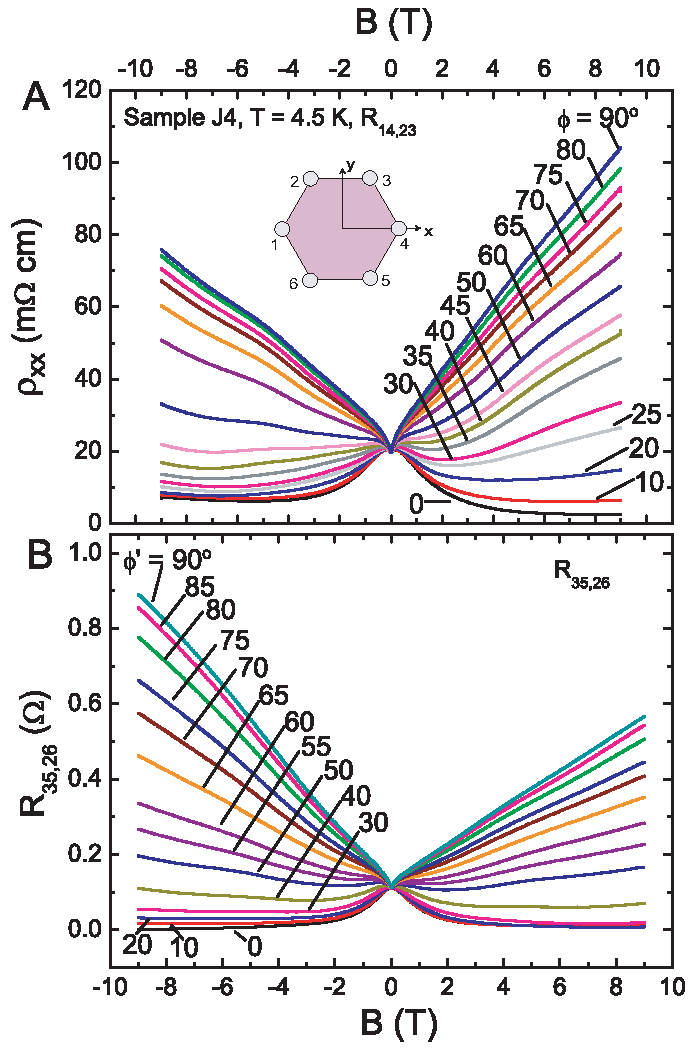
\includegraphics[width=0.75\linewidth]{ch-na3bi/figures/FigJ4RawMR.pdf}
\caption{\label{J4Raw} The unsymmetrized magnetoresistance data in Sample J4. Panel (A): The unsymmetrized MR data at 4.5 K derived from resistance $R_{14,23}$ (current $\bf{I}$ applied to the contacts (1,4) and voltage measured between contacts (2,3)). The inset shows the contact labels and the $x$ and $y$ axes fixed to the crystal. Panel (B): The unsymmetrized MR data based on resistance $R_{35,26}$. The raw data has a small antisymmetric part that we attribute to a small Hall signal inadvertently caused by misalignment between the field tilt plane and the crystal's $a$-$b$ face. Despite this small Hall signal, the negative MR is prominent in both cases when $\phi$ (or $\phi'$) is close to zero.}
  \end{center}
\end{figure}

Many semimetals have a small carrier density $n$ and a high mobility ( e.g. $\mu>$ 20,000 cm$^2$/(Vs)). According to the Drude model, the Hall angle for a one-band metal is $tan \theta_{H} = \mu B$, which increases linearly with the mobility. It indicates that the Hall resistivity $\rho_{yx}$ may become comparable to or even exceed the longitudinal resistivity $\rho_{xx}$. As observed in many of such semimetals, the magnitude of $\rho_{yx}$ indeed greatly exceeds $\rho_{xx}$ (in the standard Hall configuration with current $\bf I||\hat{x}$ and $\bf B||z$). To reduce the influence of the Hall signal, $\bf B$ is aligned to the $x$-$y$ plane as well as possible in most of our experiments. In an ideal case, the Hall effect should be zero when $\bf B$ is parallel to our sample plane. Nevertheless, the experimental data show that  the field-antisymmetric Hall signal is often observed in the background and can be comparable to the resistive voltage above 10 Tesla. One explanation for the mixing is the misalignment of the sample's $a$-$b$ plane to the field rotation plane, thus unintentionally introducing a $z$ component to $\bf B$. Though the misalignment may be small, the remnant $B_z$ could still generate a Hall component that is comparable to $\rho_{xx}$. Since the ideal MR curves are symmetric in field, the mixing of a Hall signal could easily be found from the antisymmetric part of the raw MR curves. Thus a serious misalignment may lead to a large field anti-symmetric distortion in the raw MR curves, making them tilt dramatically towards, say, the $+B$ axis. This mixing effect could be a major source for the observed ``negative resistance'' ($E_{x}<0$ for $\bf I||\hat{x}$) sometimes encountered in semimetal magnetoresistance experiments performed in large $\bf B$. When not treated appropriately, such distortions may imitate a negative MR when the raw curves are symmetrized in field. 

Therefore, to rule out the above possibility of the apparent negative MR caused by Hall mixing, it is important to examine the raw MR curves as well. Here we display the raw MR curves (pre-symmetrization) in Fig. \ref{J4Raw}. They demonstrate that the distortion discussed above is a relatively weak effect in our experiment. When the current $I$ is applied to contacts (1,4) (the measured resistance is $R_{14,23}$), the unsymmetrized raw MR curves measured in Sample J4 are displayed in Figure \ref{J4Raw}A. When $I$ is switched to the contacts (3,5) (measured resistance $R_{35,26}$), the corresponding ``rotated'' curves are exhibited in Figure \ref{J4Raw}B. In Panel A (B), $\phi$ ($\phi'$) denotes the angle between $\bf{B}$ and $\bf\hat{x}$ ($\bf\hat{y}$), following our previously defined notations. Both panels show a small asymmetry in the MR curves, which is caused by a Hall ``pick up'' signal. However, the mixing Hall signal is apparently too small to generate the large, negative MR observed when $\bf B || \bf I$.

\begin{figure}[!htbp]
  \begin{center}
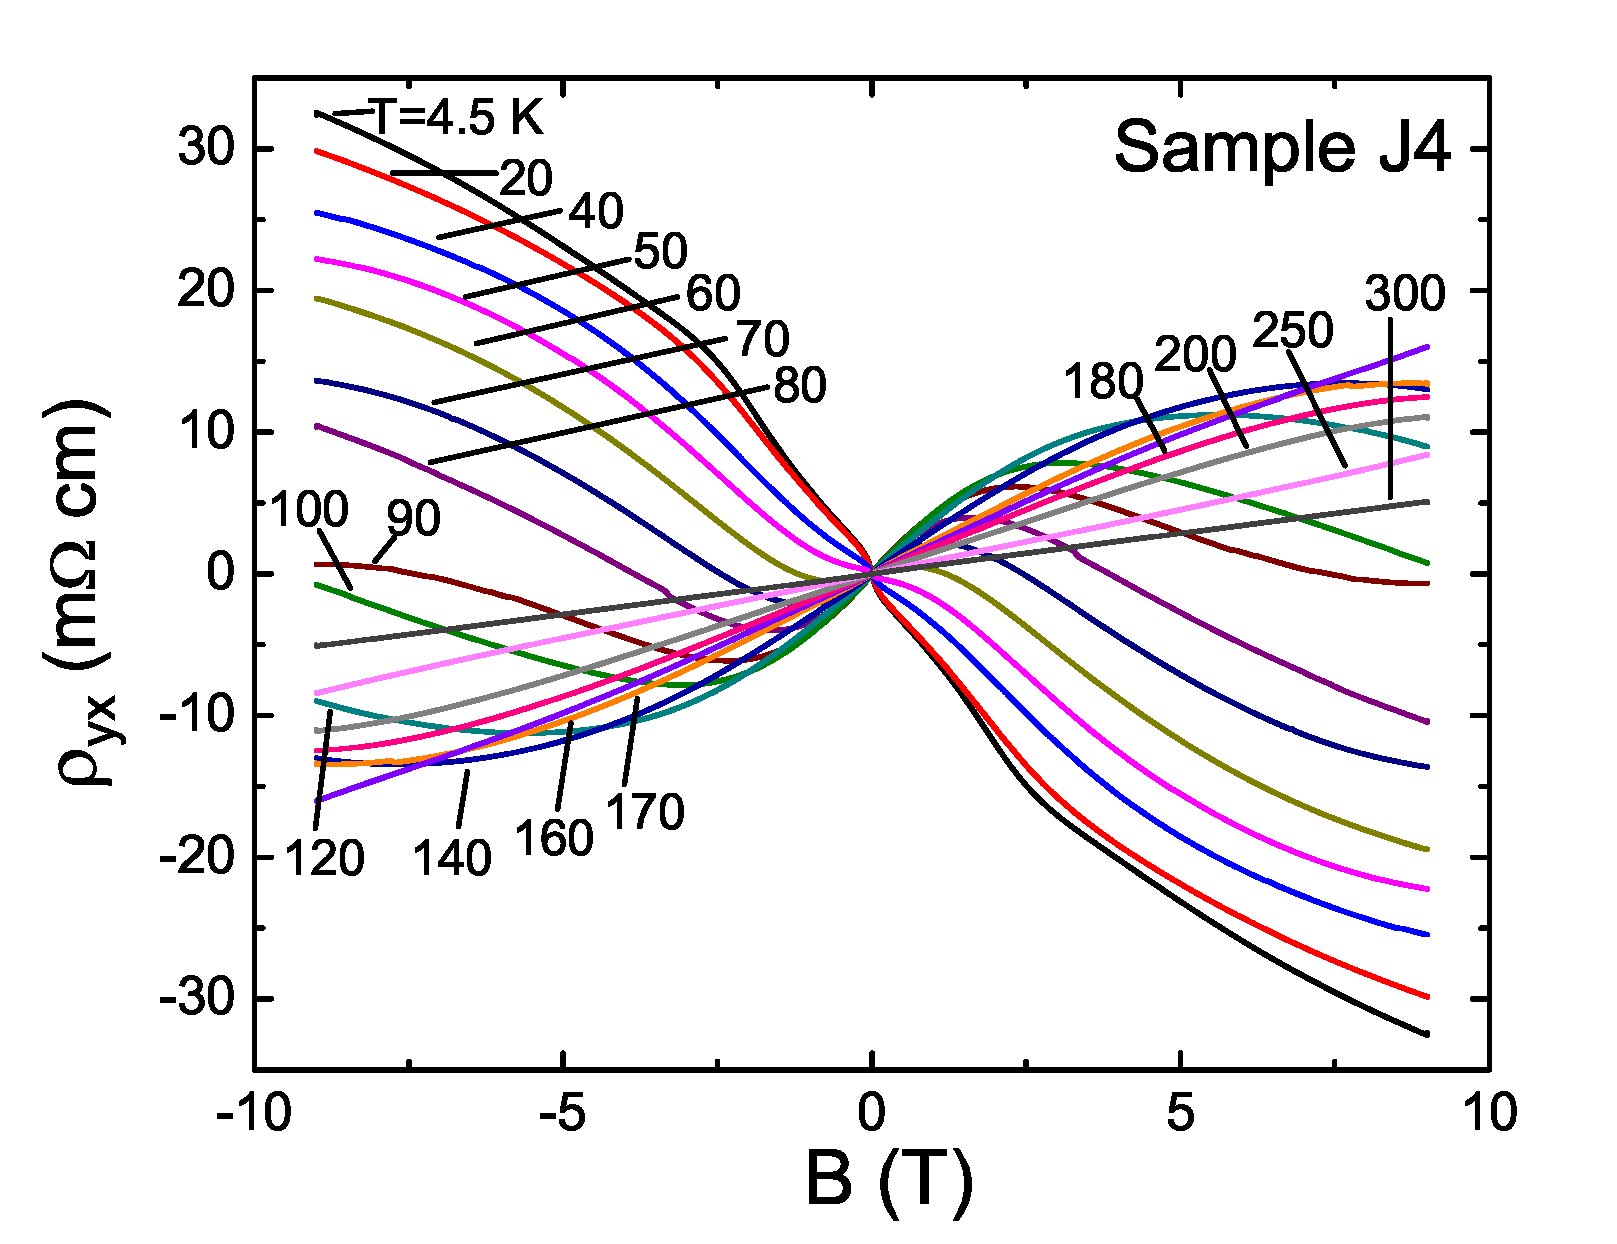
\includegraphics[width=0.8\linewidth]{ch-na3bi/figures/FigJ4Hall.eps}
\caption{\label{J4Hall} The Hall effect data of J4 at different temperatures. The Hall curves at various temperatures reveal a clear signature of thermally excited holes at high temperatures. Above 70 K, the holes start to contribute to the Hall effect and they finally dominate the Hall signal above 140 K. The conductivity enhancement in MR also disappears around the same temperature range.}
  \end{center}
\end{figure}

Figure \ref{J4Hall} shows Hall data at various temperatures in Sample J4, when $I$ is applied to the contacts (1,4) and $\bf{B}$ is parallel to the $c$-axis. The negative slopes at low temperatures indicate electrons' dominance at these temperatures. But when the temperature increases, the hole contribution grows rapidly. The hole contribution could be seen clearly even at a small $\bf{B}$ above 70 K, and it eventually dominates completely above 140 K. This hole excitation behavior is consistent with our estimation of the Fermi energy $\epsilon_F\sim$ 30 mV which is near the Dirac node (Fig. \ref{figWeyl}A). When $T$ is raised above 100 K, the steep increase of both electron and hole densities leads  to the occupation of higher Landau levels (which are not chiral), making the axial current difficult to resolve (Fig. \ref{figWeyl}D).

\begin{figure}[!htbp]
  \begin{center}
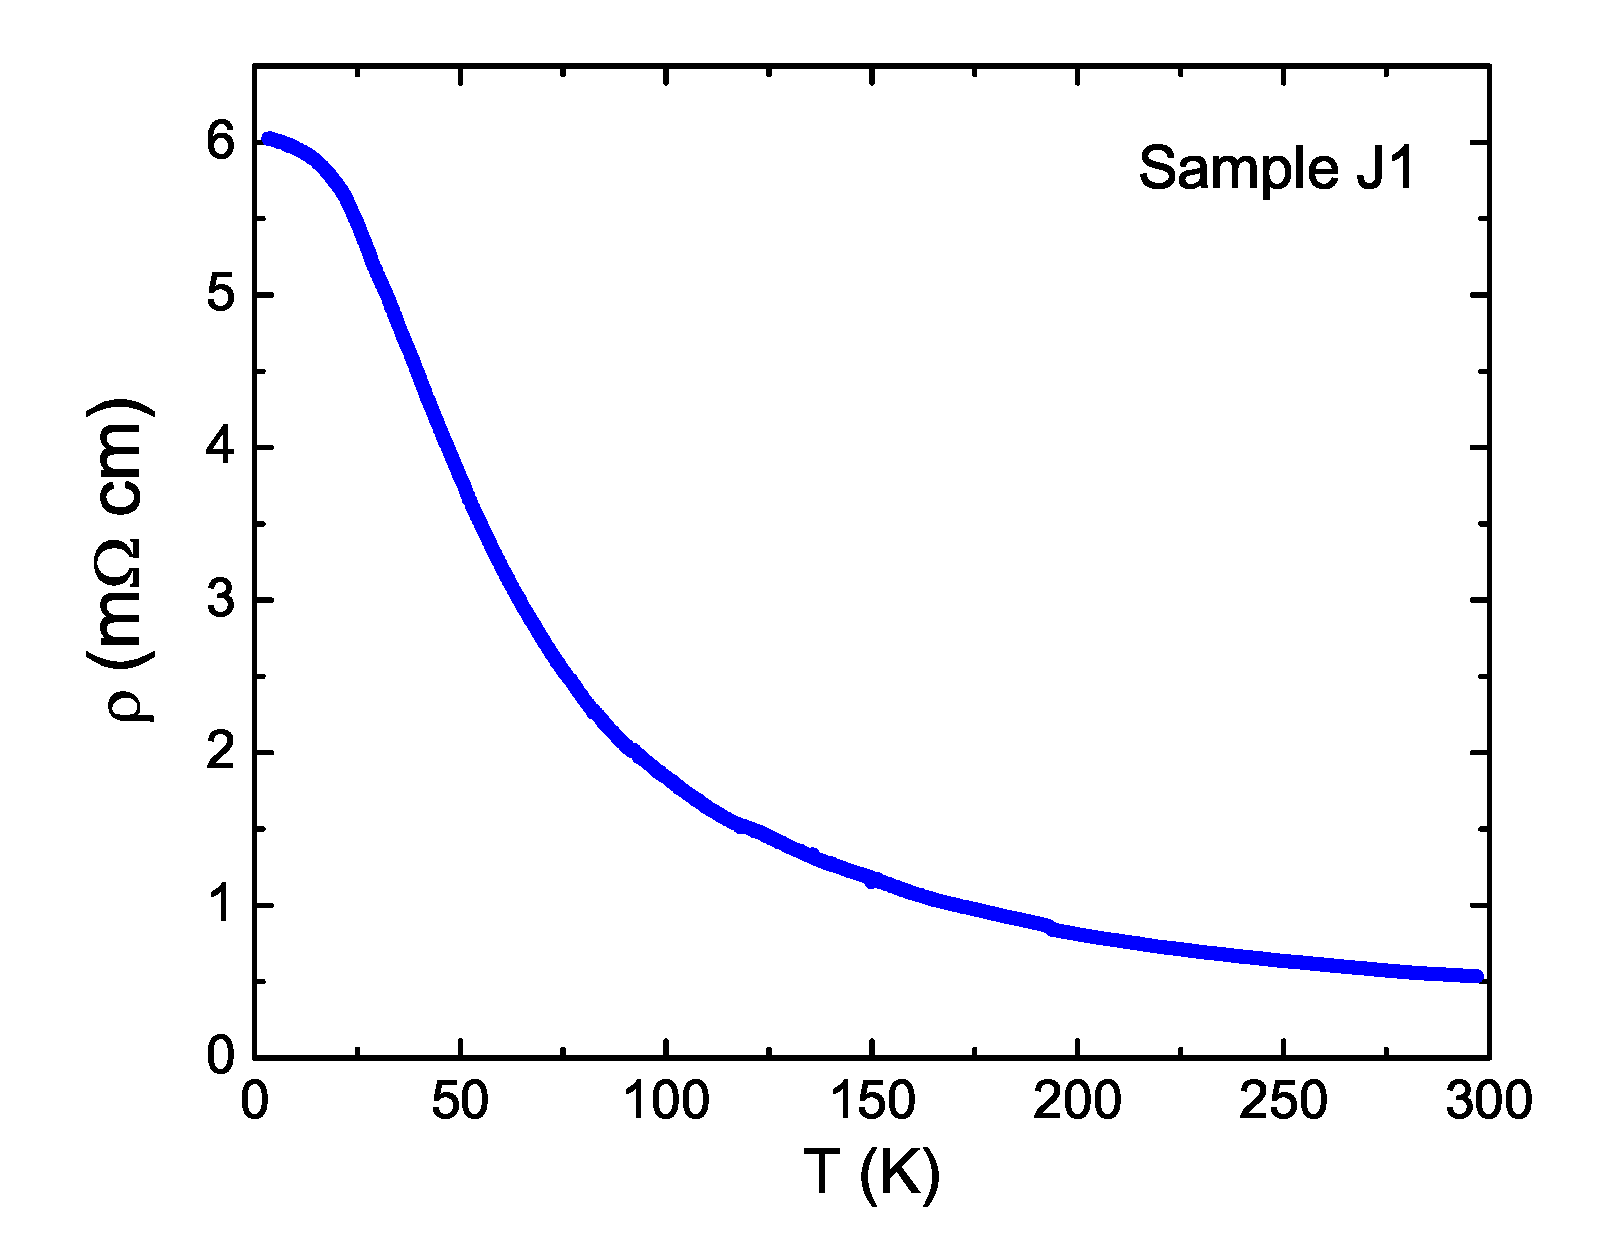
\includegraphics[width=0.75\linewidth]{ch-na3bi/figures/FigJ1rho.eps}
\caption{\label{J1rho} 
Temperature dependence of the resistivity $\rho$ in Sample J1 in zero $B$. The non-metallic profile, closely similar to that in J4, is consistent with
the freezing out of hole excitations as $T\to$ 4 K. 
}
  \end{center}
\end{figure}

\subsection{Negative Longitudinal Magnetoresistance in a Second Sample}
Below we will discuss the transport results on our second sample, J1, which shows behavior similar to that of J4. Both samples were grown within the same boule. Fig.\ref{J1rho} displays J1's non-metallic $\rho-T$ dependence. As in J4, $\rho$ saturates at a peak below 10 K as the hole contribution is frozen out. The value of $\rho$ at 4 K is about 4$\times$ smaller than that in J4. 


The longitudinal magnetoresistance $R_{14,23}$ with $\bf B||\hat{x}$ are shown in Fig. \ref{J1MRT}. When $B$ $<$ 4 T, we observe a large negative MR peak centered at $B$=0 T that gradually disappears when $T$ rises from 3.5 to 120 K. This pattern is similar to the behavior observed in J4, as it hosts a large axial current in the lowest Landau level (LL) which is overwhelmed by contributions from higher LLs at higher $T$. At very large $B$ ($>$ 20 T), the distortion caused by an unintended $z$ component $B_z$ appears in MR curves. 
We measured J1 before J4, and thus we were unaware of the critical alignment conditions needed to isolate the anomalous axial current. Also as no two-axis rotator is available for our field-rotation measurement, the misaligned $z$ component of $\bf B$ might be significant enough to suppress the axial current, even as the field is rotated in the nominal ``$x$-$y$'' plane. 

%%%%%%%%%%%%%%%%%%%%%%%%%%%%%%%%%%
%%%%%%%%%%%%%%%%%%%%%%%%%%%%%%%%%% FIGURE 3
\begin{figure}[!htbp]
  \begin{center}
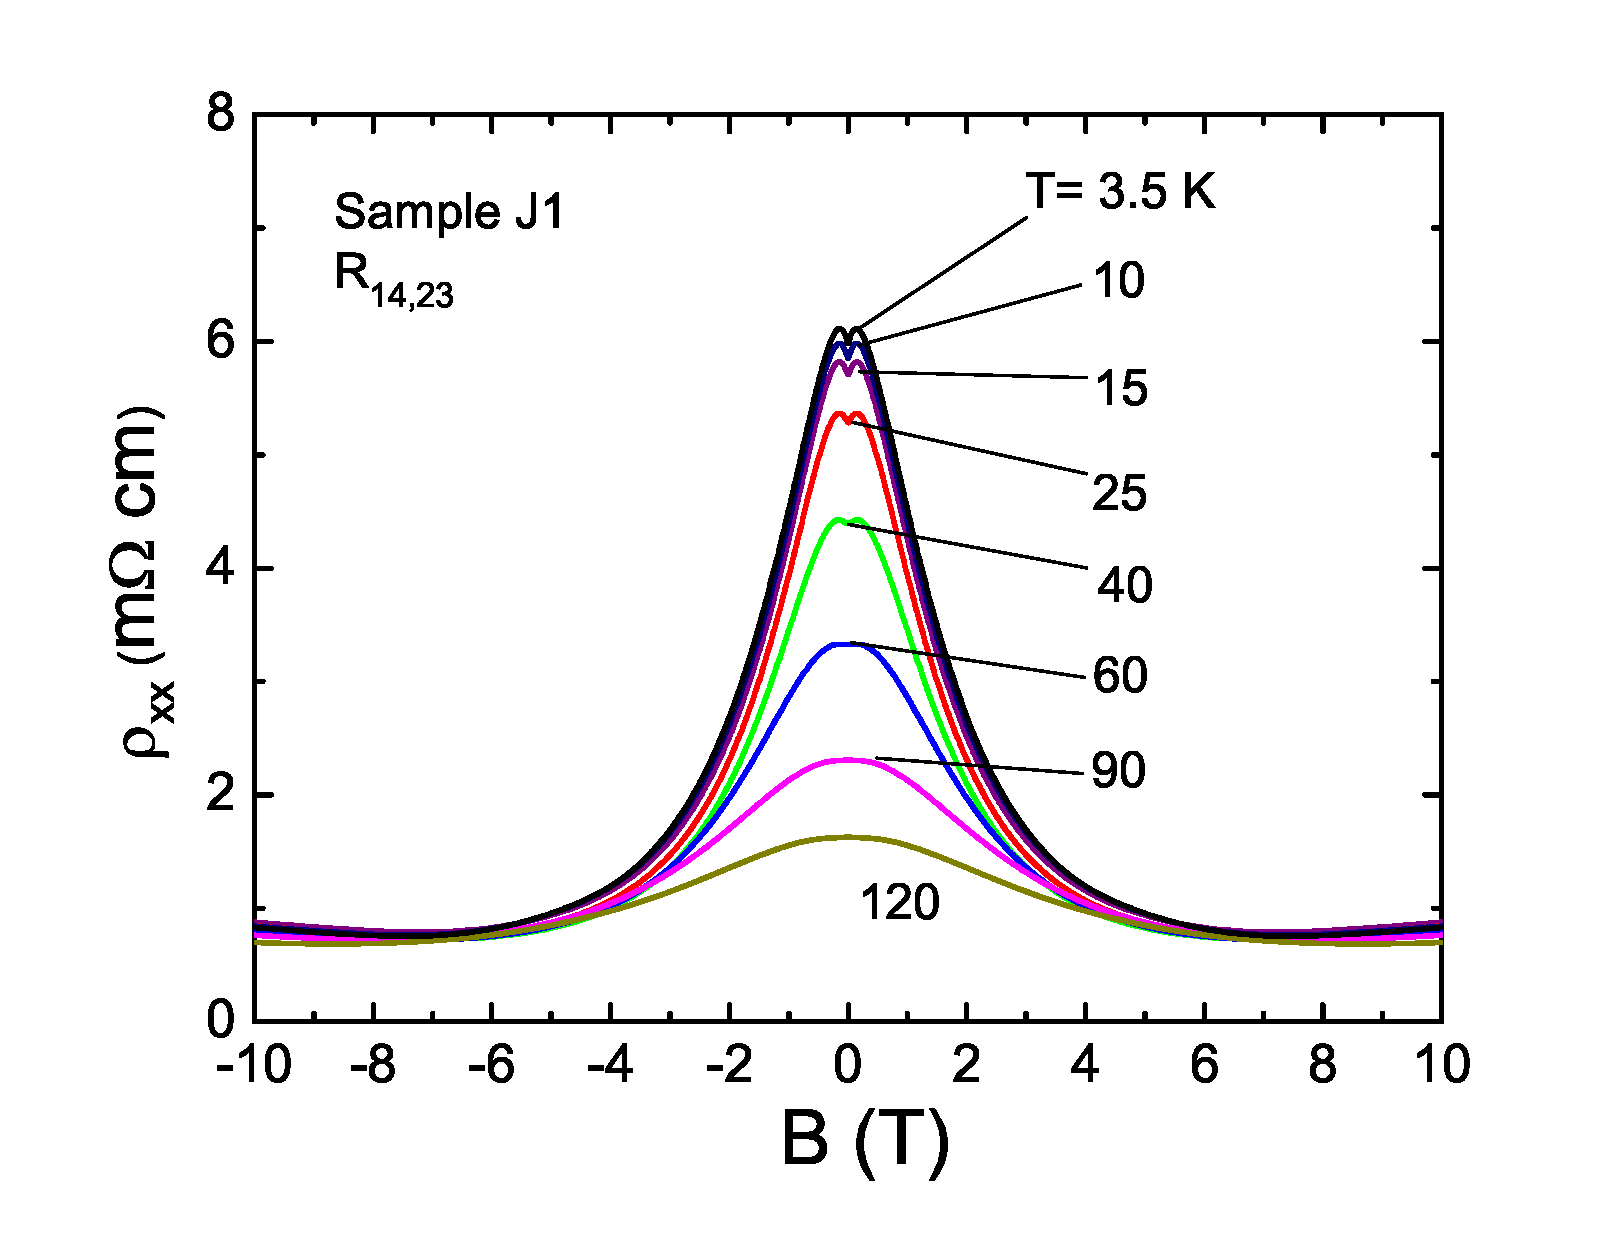
\includegraphics[width=0.9\linewidth]{ch-na3bi/figures/FigJ1MRvsT.eps}
\caption{\label{J1MRT} 
Large negative, longitudinal MR at 3.5 K observed by measuring $R_{14,23}$ with $\bf{B}||\bf\hat{x}$. The negative MR at low fields implies strong increase in the conductance when $\bf{B}||\bf{E}$. As $T$ is raised to 120 K, the negative MR anomaly is progressively suppressed as the conductance of states in upper Landau levels become dominant. The very small increasing background discernible above 7 T reflects a small $B_z$ caused by misalignment.}
  \end{center}
\end{figure}


%%%%%%%%%%%%%%%%%%%%%%%%%%%%%%%%%%
%%%%%%%%%%%%%%%%%%%%%%%%%%%%%%%%%% FIGURE 3




\begin{figure}[!htbp]
  \begin{center}
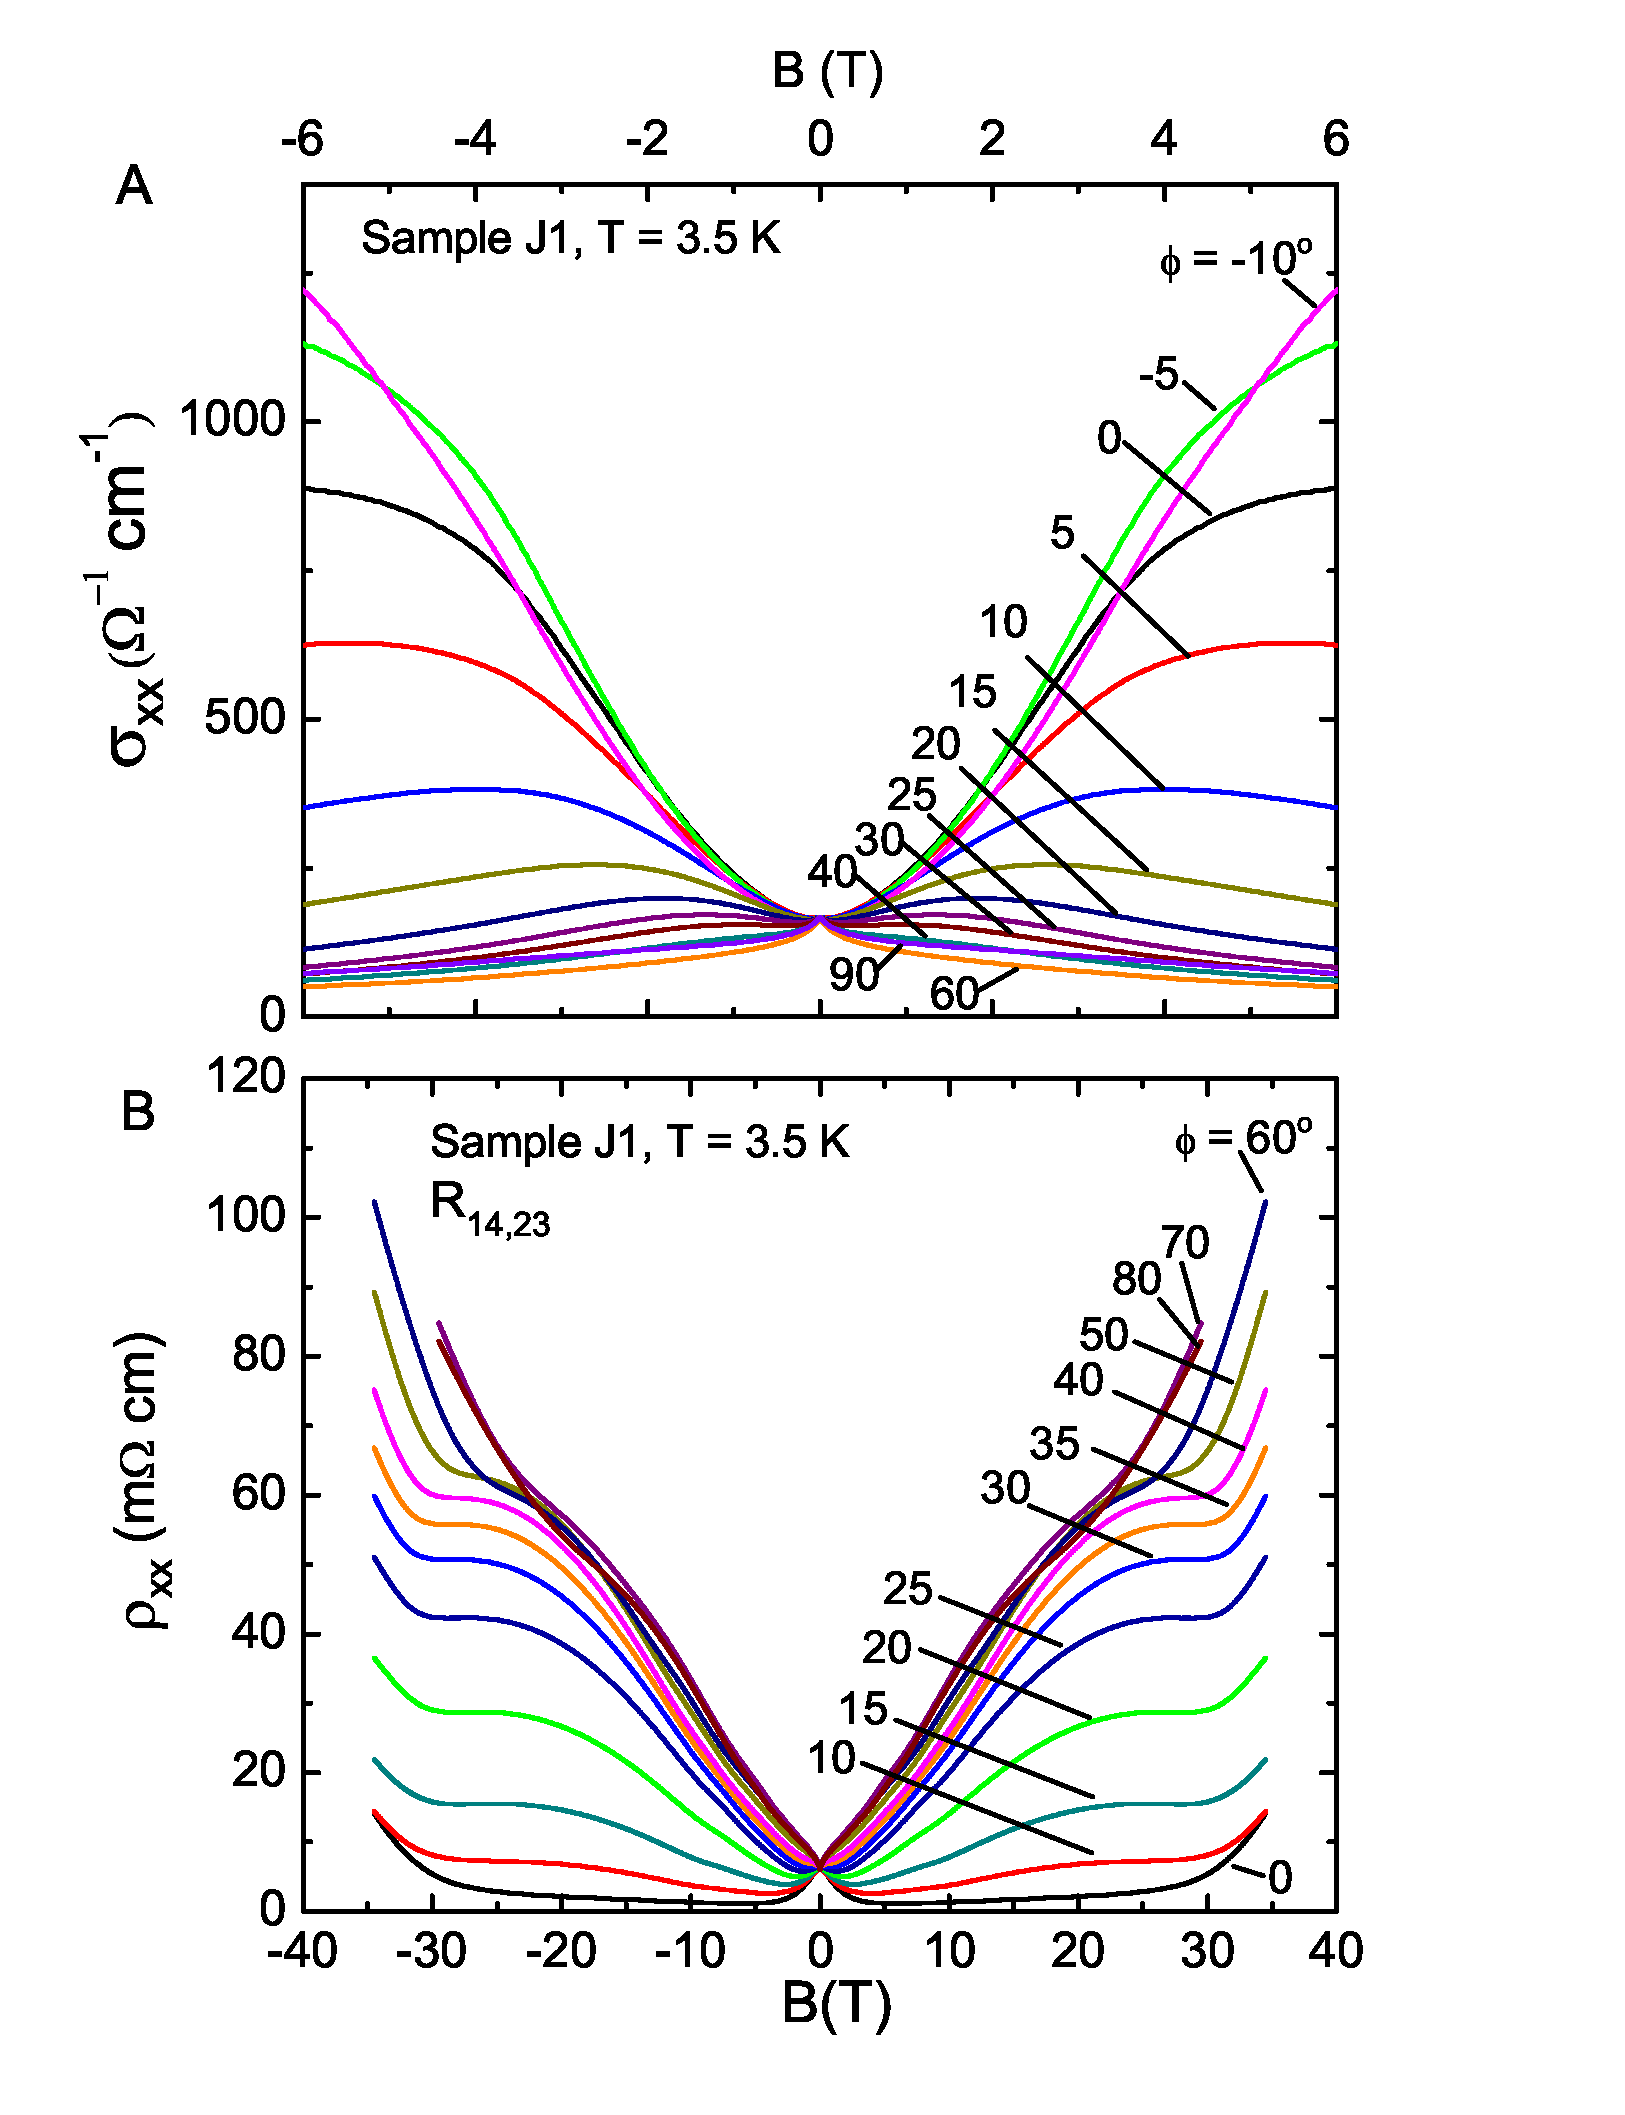
\includegraphics[width=0.8\linewidth]{ch-na3bi/figures/FigJ1CondMR.eps}
\caption{\label{J1MR} Panel (A): Variation of the conductivity curves $\sigma_{xx}(\phi)$ vs. $B$ at selected tilt angles $\phi$ in Sample J1 at $T$ = 3.5 K. 
$\sigma_{xx}(\phi)$ is derived from measurements of $R_{14,23}$. As $\phi$ is rotated to close to 0, $\sigma_{xx}$ increases strongly as $B^2$ consistent with Eq. \ref{eq:SS}. We identify this with the axial current. 
Panel B shows the curves of $\rho_{xx}$ vs. $B$ measured in J1 at 3.5 K at selected tilt angles $\phi$ in fields up to 35 T. The profiles are similar to those shown in Fig. \ref{figMR4}D for Sample J4. A kink feature appears at $H_k$ in the rangle 30-35 T, above which $\rho_{xx}$ increases steeply. Here, the $\phi = 0$ curve (for J1) is also affected by $H_k$ (unlike in J4), possibly because of the larger misalignment in J1.
}
  \end{center}
\end{figure}

Fig. \ref{J1MR}A displays the conductivity $\sigma_{xx}$ v.s. $B$ curves (in J1), which are derived from measurements of $R_{14,23}$, when $\bf B$ is lying in the $x$-$y$ plane (at an angle $\phi$ to $\bf\hat{x}$). As in Sample J4, the conductivity follows a strong $B^2$ enhancement when $\phi$ is close to 0, which is consistent with Eq. 2. Fig. \ref{J1MR}B shows the resistivity $\rho_{xx}$ v.s. $B$ curves measured up to 35 T. Similar to J4, there is a large and positive MR when $\bf B$ is perpendicular to $\bf I$ (curves at 80$^\circ$). But the MR gradually becomes negative as $\phi$ approaches 0$^\circ$. We estimate the misalignment between the $a$-$b$ plane and the field-tilting plane in J1 to be $(10\pm 3)^\circ$. The misalignment has another signature in the MR above 30 T. As discussed previously, a knee feature appears at the kink field $H_k\sim$ 30-35 T in Sample J4, above which $\rho_{xx}$ grows rapidly. The $H_k$ of J4 shifts strongly with $\phi$. When $\phi < 25^\circ$ it increases above 35 T (see Fig.\ref{figMR4}D), making the $\phi=0$ curve unaffected. In Sample J1, we also see a similar kink behavior at high fields. Nevertheless, $H_k(\phi)$ in J1 has a milder dependence on $\phi$ in Fig. \ref{J1MR}B. In particular, a small upturn is observed above 30 T in the 0$^\circ$ curve. We interpret this as an implication of a non-negligible $B_z$ component in the measurement at $\phi$ = 0. 

Therefore, in J1, we have observed the main features of the MR data reported for J4 in the previous section. However, above 30 T, the larger misalignment of the crystal plane in J1 leads to an upturn in $\rho_{xx}$ that does not appear in J4. Comparison of the MR results from J1 and J4 in the large-$B$ limit also implies that the angular width of the collimated beam generated by the axial current is narrow. 



%\centerline{*     *     *}\vspace{6in}


\subsection{Resistivity and Conductivity Tensors from Boltzmann Equation in a Tilted Magnetic Field}
In this subsection, we will show that the above MR results of our Na$_3$Bi samples at different directions of $\bf B$ are not expected from the conventional semiclassical, one-band transport theory in a tilted field. Considering a single anisotropic band, the Boltzmann equation that describes the transport pheomena is
\be
e{\bf E\cdot v}\frac{\partial f^0_{\bf k}}{\partial \epsilon_{\bf k}} + e{\bf v\times B}\cdot\frac{\partial g_{\bf k}}{\partial {\bf k}} 
= -\frac{g_{\bf k}}{\tau},
\label{Boltz}
\ee
where $e$ is the electron charge, $\bf E$ is the electric field, $\bf v = \partial\epsilon_{\bf k}/\hbar\partial {\bf k}$ is the Fermi velocity of Bloch electrons, $g_{\bf k}$ is the leading correction to the equilibrium distribution function $f^0_{\bf k}$, and $\tau$ is the relaxation time. We assume that the magnetic field is tilted in the $x$-$z$ plane, i.e. ${\bf B} = (B_1, 0, B_3)$. Using the \emph{ansatz} with $\bf u$ the drift velocity
\be
g_{\bf k} = -{\bf u\cdot k}\frac{\partial f^0_{\bf k}}{\partial \epsilon_{\bf k}},
\ee
and the effective mass matrix
\begin{eqnarray}
\hat{m} = \left[   \begin{array}{ccc}
		m_1   &   0   &   0 \\
		0      &    m_2 &   0 \\
		0     &    0     &   m_3   \end{array}\right]
\end{eqnarray}
we can solve Eq. \ref{Boltz} to obtain the resistivity tensor ($n$ is the carrier density)
\begin{eqnarray}
\hat{\rho} = 
						\left[  	\begin{array}{ccc}
								\rho_1	&  -B_3/ne   &   0  \\
								B_3/ne  &   \rho_2   &   -B_1/ne \\
								0          &   B_1/ne   &   \rho_3   
								\end{array}
								\right].
				\label{rhoij}
				\end{eqnarray}
				

The conductivity tensor can be obtained by inverting $\hat\rho$, which is 
\begin{eqnarray}
\hat{\sigma} = 
						\frac{1}{\Delta}\left[  	\begin{array}{ccc}
								\sigma_1(1+\mu_1\mu_3 B_1^2)  &  \sigma_1\mu_2B_3   &   \sigma_2\mu_1\mu_3 B_1B_3 \\
								 -\sigma_1\mu_2B_3									&   \sigma_2   									&   \sigma_2\mu_3B_1   \\
								\sigma_2\mu_1\mu_3 B_1B_3     &    -\sigma_2\mu_3B_1      &   \sigma_3(1+\mu_1\mu_2B_3^2)
								\end{array}
								\right]
				\label{Sij}
				\end{eqnarray}
where the elements of the conductivity and resistivity tensors at $B$=0 are defined by $\sigma_i = 1/\rho_i = ne\mu_i $. Here the anisotropic
mobilities are $\mu_i = e\tau/m_i$. The determinant $\Delta$ equals $(1+\mu_2\mu_3 B_1^2+ \mu_1\mu_2 B_3^2)$.

The above equations describe how different elements of the conductivity and resistivity tensors depend on the direction of $\bf B$. An important conclusion is that, despite the anisotropy and the tilted field direction, the longitudinal resistivity 
$\rho_{xx}$ (the three diagonal terms) is strictly independent of $\bf B$, indicating the perfect balance between the Hall E-field and the Lorentz force. In the limit $B_3\to 0$ (or $\theta\to 0$ in Fig. \ref{figPolar4}C,D), the longitudinal conductivity $\sigma_{xx}$ follows a mild field dependence that vanishes if $\mu_1 = \mu_2 = \mu_3$. Therefore, $\sigma_{xx}$ only varies slowly with $\theta$, and it never diverges as $1/\sin\theta$ or any other sharp form.

Equations \ref{rhoij} and \ref{Sij} also apply to the configuration with $\bf B$ tilted in the $x$-$y$ plane (Fig. \ref{figMR4} and Fig. \ref{figPolar4}A,B in previous subsections) if we exchange the axes $y\leftrightarrow z$.


\subsection{Splitting of Generated Weyl Nodes of a Dirac Semimetal in a Magnetic Field}
In this subsection, we will discuss a crucial problem of 3D Dirac semimetals, i.e. how much shift can the Weyl nodes have when they are split by a magnetic field . To solve this problem,we leverage the model introduced by Wang \etal~\cite{Wang2012} (see also Jeon \etal~\cite{Jeon2014}), and estimate the shift of the Weyl nodes induced by the magnetic field $\bf B$ as follows. In a field $\bf B\parallel \hat{z}$, we have ${\bf k \to \Pi} = {\bf k} - e{\bf A}$, with the vector potential ${\bf A} = xB{\bf \hat{y}}$. The wavevector $\bf k$ is measured relative to the Dirac node. Neglecting the off-diagonal corrections in the full $4\times4$ Hamiltonian, we can work in the
$2\times2$ matrix of the Hamiltonian for the ``up'' Weyl node with the form 
\begin{eqnarray}
H_+ = \hbar v\left[\begin{array}{cc}
						\Pi_z   &  \Pi_+   \\
						\Pi_-   &   -\Pi_z  
						\end{array}\right]
						-\mu_B B \left[\begin{array}{cc}
						g_s   &   0   \\
						0      &   g_p  
						\end{array}\right],
						\label{H1}
						\end{eqnarray}
where $\Pi_{\pm} = \Pi_x \pm i\Pi_y$ and $\mu_B$ is the Bohr magneton. We can also write the $g$-factors $g_s$ and $g_p$ (which are distinct) of the starting atomic orbitals $|S,\pm\rangle$ and $|P,\pm\rangle$ as $g_s = g_m + \delta g$ and $g_p = g_m - \delta g$. Then the Hamiltonian becomes
\be
H_+ = v{\bf \Pi\cdot }\boldsymbol{\tau} - g_m\mu_B B {\bf 1}- \delta g\mu_B B \tau_3,
\label{H2}
\ee
where $\tau_i$ are the Pauli matrices in orbital space.
To solve it for the energy spectrum, we transform the $\Pi_\pm$ to the raising and lowering operators $a^\dagger$ and $a$, with $\ell_B$ the magnetic length,
\be
\Pi_+ = \frac{\sqrt{2} a^\dagger}{\ell_B}, \quad \Pi_- = \frac{\sqrt{2} a}{\ell_B}
\label{Pi}
\ee
then we diagonalize $H_+$ to obtain the eigenenergy of the $n^{th}$ Landau level
\be
E_n(k_z) = -g_m\mu_B B \pm \sqrt{ \frac{2n\hbar^2 v^2}{\ell_B^2} + (\hbar vk_z -\delta g\mu_BB)^2}.
\label{En}
\ee
To find the splitting of the Weyl nodes, we set the second term under the square root to zero and obtain $\Delta k = \delta g\mu_B B/\hbar v$. Thus the splitting grows linearly with the magnetic field. We also notice that the magnitude of the splitting depends on the difference of the $g$-factors of the two orbits. This is the expression we use in the previous sections to estimate the shift. Consistent with Fig. \ref{figSdH}, the term $-g_m\mu_B B$ in Eq. \ref{En} results in pronounced deviation of the index plot from a straight line if $|g_m|\gg 1$.

\subsection{The Negative MR does not Origin from Localization}

In this subsection, we will demonstrate our evidence that the observed negative LMR cannot be interpreted by localization. Negative MR is not uncommon in the transport experiments of metals. The well-established Anderson localization theory can well explain the negative MR in 2D disordered metals. However, we believe it is irrelevant to the negative LMR in our Na$_3$Bi. We discuss the reasons below.

Here we briefly review the picture of Anderson localization. When electrons diffuse in a disordered metal at very low $T$, the transmission amplitude $\mathcal{A}$ between two points P and P$'$ is the sum of contributions over all Feynman paths linking P to P$'$. We may consider an electron's path that forms a loop and returns to the origin. In a diffusive system, the loop size L is much larger than the electron mean-free-path $\ell$. In this loop, the electron can be scattered by several impurities. An electron can travel clockwise or anticlockwise on the loop, and the two paths form a time-reversal partner for each other. Since these two paths always have the same phase and interfere constructively, their amplitudes are greatly enhanced, especially compared to other random-averaged paths. As a result, the electrons are more likely to be restricted inside these paths and it leads to Anderson localization. Such phenomena are more distinct at lower temperatures when the inelastic scattering with phonons is suppressed. At a high temperature, the phonon scattering destroys the quantum coherence and makes L decrease rapidly. In a 2D system, the weak localization results in the log$T$ increase of the resistance. For 3D metals, $R$ varies as $T^{-n}$ (n = $\frac14$ $\to$ $\frac12$ ).

When a magnetic field is applied, the phases of the clockwise or anticlockwise paths will differ. Thus the constructive interference is steeply reduced. Therefore, the MR becomes negative as the localization effect is weakened by $\bf B$. In 2D, $\Delta R$ follows a -log$|B|$ dependence in a low field while it varies as $B^{-\frac12}$ in 3D. In 2D metals, the characteristic field decreases from 100 G at 2 K to 20 G at 100 mK, as $L$ increases. There are many experiments showing the weak localization effect in 2D. Nevertheless, this effect is rare in 3D systems, since the Feynman paths in 3D seldom self-intersect and the quantum correction term is not large.

% Since different paths interfere with each other, some paths almost cancel each other's contribution from P to P$'$ in zero magnetic field. 
%If we invert one of these two paths, we will see that the two paths form a closed loop and the amplitude doubles. Such closed loops indicate that electrons have a lower probability to transmit to other positions and thus become localized. In a modest magnetic field, the phase in the loops are tuned by the magnetic field and the amplitudes of these localized loops decrease. Thus it can cause a negative MR.


%The diffusive nature of electrons moving in a sea of impurities dictates that the size L of a closed loop is generally $\gg$ $\ell$, the electron mean-free-path. In zero $B$, the 2 paths traversing a closed loop (clockwise v.s. anticlockwise) are exact time-reversed partners. Hence
%wave packets following the two paths must interfere constructively when they return to the node regardless of $L$. Consequently, the amplitude for observing the electron at the node is enhanced, leading to Anderson localization. Because raising $T$ increases inelastic scattering by phonons (which destroys the quantum coherence), $L$ shrinks rapidly with increased $T$. As $T$ decreases, the quantum corrections lead to a resistance $R$ that increases as log$T$ in 2D. For 3D metals, $R$ varies as $T^{-n}$ (n = $\frac14$ $\to$ $\frac12$ ). In finite $B$, the constructive interference is suppressed once the magnetic flux in $L^2$ exceeds $\sim$ $\frac12$ a flux quantum $\phi_0$. As noted, this leads to a negative MR,with $\Delta R$ $\sim$ log$B$ in 2D. In 3D,$\Delta R$ $\sim$ $B^{-\frac12}$. In 2D metals, the characteristic field decreases from 100 G at 2 K to 20 G at 100 mK, as $L$ increases. Experimentally, 2D localization has been extensively investigated. In 3D metals, however, it has been difficult to observe in MR experiments. The corrections are weak presumably because Feynman paths in 3D rarely self-intersect.

The following are the reasons why we believe localization is not relevant in our Na$_3$Bi samples:

First, the $\rho$ v.s. $T$ curve in $B$ = 0 (Fig.\ref{figWeyl}C) shows that $\rho$ increases by a factor of $\sim$ 12 when $T$ decreases from 300 K. The large variation $\Delta \rho$ between 30 and 100 K is matched by a large change in $R_H$ as we measured. It indicates that the increase in $\rho$ as $T$ decreases results from the frozen holes across the zero gap in Na$_3$Bi rather than Anderson localization (which should not be observable above a few K in 3D either). The $\rho$ v.s. $T$ curve also saturates to a constant below 25 K, contradicting with the prediction of localization that suggests a continuous and sharp increase of $\rho$ as T $\to$ 0 K. 

Second, the localization effect in a 3D metal is rather isotropic in $\bf B$ while the axial current in Na$_3$Bi has a noticeable angular anisotropy when $\bf B$ tilts. For example, Figs. \ref{figMR4} and \ref{figPolar4} show that the large negative LMR can only be observed when $\bf B$ is aligned to $\bf I$ within 3-5 degrees. The steep suppression of the axial current when $\bf B$ deviates from $\bf E$ cannot be explained by the 3D localization, since the quantum interference in 3D localization is equally reduced by $\bf B$ from different directions. In addition, the negative LMR persists up to 90 K, while the 3D localization effects usually happen below 2 K.

Third, the overall change of $\rho_{xx}$ in the negative MR profile of Na$_3$Bi (Fig. \ref{J1MRT} and Fig. \ref{figWeyl}D of main text) is much larger than that in a typical localization system. $\rho_{xx}$ decreases by a factor $>$ 5 at 4 K in Na$_3$Bi. By contrast, the decrease in a typical 2D localization system is within a few \% while the change is even smaller in 3D case. Also, the field scale $B_{\omega}$ needed to suppress the peak in $\rho_{xx}$ is 3-4 T for Na$_3$Bi, much larger than the $<$100 Oe field that is typical in localization experiments. Furthermore, if the negative MR were indeed induced by the localization, then the typical loop size would be $L = \sqrt{\phi_0/2B_{\omega}} \simeq 25$ nm at 4 K, but such a small L could not produce the pronounced 5$\times$ change in $\rho_{xx}$. Moreover, such a small $L$ implies a very short mean free path $\ell$, inconsistent with the measured mobility ($\mu$ = 2600 cm$^2$/(Vs) at 4 K).

\section{Summary}
\label{sec:na3bi:summary}


We have discussed our transport study of two types of Na$_3$Bi crystals in this chapter. The first type of Na$_3$Bi has a high $E_F$ and displays a linear MR when $\bf B$ is perpendicular to $\bf I$. The Hall angle in these samples displays a step-function behavior and indicates that the transport lifetime is surprisingly sensitive to the magnetic field. In the second type, $E_F$ is close to the Dirac point and we have observed a negative longitudinal magnetoresistance when $\bf B$ is parallel to $\bf E$. Such negative LMR follows a quadratic $B$ dependence as proposed by the theoretical prediction for the axial current induced between Weyl fermions \cite{Son2013}. In addition, the negative LMR can be lifted with a very small deviation of the $\bf B$ direction. The chiral anomaly effect in a WSM or DSM is predicted to be weaker when the angle between $\bf B$ and $\bf E$ increases. But the previous theoretical study has not given a formula for the angular sensitivity of the caused negative LMR. The ultra sensitivity we observed here may inspire future study of the suppression and scattering mechanism of the axial current in a WSM and DSM.


%%
\chapter{Usage\label{ch:usage}}

To start, in your main .tex file, use this class as your main documentclass instead of `report' or `book'. For example:
\begin{quote}
$\backslash documentclass[12pt,lot, lof]\{puthesis\}$
\end{quote}

In this example, we setup our document to use the PU Thesis style, with 12pt font for body text, and to include a List of Tables and List of Figures in the front matter. You could instead set an 11 point or 10 point font by changing the first option. You can also add `los' to include a list of symbols.

To use single spacing, add the option `singlespace'. This is a special option for the \texttt{puthesis} documentclass, which sets single spacing for both the front matter and for the document itself. Additional parameters should be set in your main .tex file, and are described in detail in Section~\ref{sec:usage:options}.

The template itself declares two other options, to be set immediately after the \texttt{documentclass} command. First is `printmode', declared with the command:
\begin{quote}
$\backslash newcommand\{\backslash printmode\}\{\}$
\end{quote}
This command, used later in the thesis.tex file, turns off the \texttt{hyperref} package and all internal links in the PDF file. This removes any colored links and highlighting that would not be appropriate in a printed and bound thesis. Instead the \texttt{url} package is loaded, so that \\url commands in your document will continue to work and urls will break properly across multiple lines.

When `printmode' is not specified, the hyperref package is included. It creates colored links for citations, footnotes, and internal references, which can be used to navigate the PDF document more easily. It also adds bookmarks to the PDF file, mirroring the table of contents. By default, it is set to use colored links. For the PDF file that you will submit electronically to ProQuest, this may not be desirable since some copies may be printed, while others will be used electronically. Thus another option, `proquestmode', is defined that keeps hyperref but disables colored links:
\begin{quote}
$\backslash newcommand\{\backslash proquestmode\}\{\}$
\end{quote}
This mode has no effect when used in combination with `printmode'. 


\section{Options}
\label{sec:usage:options}

In this section, we describe the options you can set when using this thesis class.
\tablespacing
% tablespacing is defined by the class to set single spacing for the long table when in doublespacing mode. If the singlespace option is set, this command has no effect.

\begin{longtable}{p{0.3\linewidth} p{0.6\linewidth}}

  % First page heading
  \caption[Options Provided by the PUthesis Class]{List of options for the puthesis document class and template} \label{tab:usage:options}\\
  \toprule
  \textbf{Option} & \textbf{Description} \\
  \midrule
  \endfirsthead

  % Future page heading
  \caption[]{(continued)}\\
  \toprule
  \textbf{Option} & \textbf{Description} \\
  \midrule
  \endhead

  % Page footer
  \midrule
  \multicolumn{2}{r}{(Continued on next page)}\\
  \endfoot

  % Last page footer
  \bottomrule
  \endlastfoot

  12pt &
  Specify the font size for body text as a parameter to \texttt{documentclass}. The Mudd Library requirements~\cite{muddthesis2009} state that 12pt is preferred for serif fonts (e.g., Times New Roman) and 10pt for sans-serif fonts (e.g., Arial).
  \\

  letterpaper &
  If your document is coming out in a4paper, your LaTeX defaults may be wrong. Set this option as a parameter to \texttt{documentclass} to have the correct 8.5"x11" paper size.
  \\

  lot &
  Set this option as a parameter to \texttt{documentclass} to insert a List of Tables after the Table of Contents.
  \\


  lof &
  Set this option as a parameter to \texttt{documentclass} to insert a List of Figures after the Table of Contents and the List of Figures.
  \\

  los &
  Set this option as a parameter to \texttt{documentclass} to insert a List of Symbols after the Table of Contents and the other lists.
  \\

  singlespace &
  Set this option as a parameter to \texttt{documentclass} to single space your document. Double spacing is the default otherwise, and is required for the electronic copy you submit to ProQuest. Single spacing is permitted for the printed and bound copies for Mudd Library.
  \\
  
  draft &
  Set this option as a parameter to \texttt{documentclass} to have \LaTeX mark sections of your document that have formatting errors (e.g., overfull hboxes). 
  \\

  % the cmidrule here spans both columns but is indented slightly on the left and right. 
  \cmidrule[0.1pt](l{0.5em}r{0.5em}){1-2}

  \raggedright
  $\backslash newcommand$ $\{\backslash printmode\}\{\}$ &
  Insert this command after the \texttt{documentclass} command to turn off the hyperref package to produce a PDF suitable for printing.
  \\

  \raggedright
  $\backslash newcommand$ $\{\backslash proquestmode\}\{\}$  &
  Insert this command after the \texttt{documentclass} command to turn off the `colorlinks' option to the hyperref package. Links in the pdf document will then be outlined in color instead of having the text itself be colored. This is more suitable when the PDF may be viewed online or printed by the reader.
  \\

  $\backslash makefrontmatter$ &
  Insert this command after the \texttt{$\backslash begin\{document\}$} command, but before including your chapters to insert the Table of Contents and other front matter.
  \\
  
  \cmidrule[0.1pt](l{0.5em}r{0.5em}){1-2}

  $\backslash title$ &
  Set the title of your dissertation. Used on the title page and in the PDF properties.
  \\

  $\backslash submitted$ &
  Set the submission date of your dissertation. Used on the title page. This should be the month and year when your degree will be conferred, generally only January, April, June, September, or November. Check the Mudd Library rules~\cite{mudd2009} for the appropriate deadlines.
  \\

  $\backslash copyrightyear$ &
  Set the submission year of your dissertation. Used on the copyright page.
  \\

  $\backslash author$ &
  Your full name. Used on the title page, copyright page, and the PDF properties. \\

  $\backslash adviser$ &
  Your adviser's full name. Used on the title page. \\

  $\backslash departmentprefix$ &
  The wording that precedes your department or program name. Used on the title page. The default is ``Department of'', since most people list their department and can leave this out (e.g., Department of Electrical Engineering), however if yours is a program, set $\backslash departmentprefix\{Program in\}$ \\

  $\backslash department$ &
  The name of your department or program. Used on the title page. \\

  \cmidrule[0.1pt](l{0.5em}r{0.5em}){1-2}
  
  \raggedright  
  $\backslash renewcommand$ $\{\backslash maketitlepage\}\{\}$ &
  Disable the insertion of the title page in the front matter. This is useful for early drafts of your dissertation. \\

  \raggedright  % full justification places the * in an awkward place
  $\backslash renewcommand*\{\backslash makecopyrightpage\}\{\}$ &
  Disable the insertion of the copyright page in the front matter. This is useful for early drafts of your dissertation. \\

  \raggedright 
  $\backslash renewcommand*\{\backslash makeabstract\}\{\}$ &
  Disable the insertion of the abstract in the front matter. This is useful for early drafts of your dissertation. \\

\end{longtable}
\bodyspacing
% bodyspacing restores double spacing or single spacing after the table

% need blank space after \bodyspacing

I've seen other people print their dissertations using $\backslash pagestyle\{headings\}$, which places running headings on the top of each page with the chapter number, chapter name, and page number. This documentclass is not currently compatible with this option -- the margins are setup to be correct with page numbers in the footer, placing them 3/4" from the edge of the paper, as required. If you wish to use headings, you will need to adjust the margins accordingly.
 





\chapter{Conclusion\label{ch:conclusion}}

In this thesis, we have discussed our transport study of two types of Dirac electrons in solids, i.e. the surface electrons in a topological insulator and the 3D electrons in a Dirac semimetal. The electronic states of these two systems can both be described by the Dirac equations, in two dimensions and three dimensions respectively. The nature of these states is deeply connected to the Berry curvature and topology in the momentum space. Such characteristics in the momentum space determine many physical properties of the crystals. Through our high field transport study, we have been able to reveal some of the novel properties induced by the exotic topological structure in these crystals.

By studying a bulk-insulating TI Bi$_2$Te$_2$Se, we have been able to demonstrate prominent quantum oscillations from its Dirac surface states. We have synthesized Bi$_2$Te$_2$Se crystals based on the chemical doping method and have obtained one of the most bulk-insulating topological insulators. Hence, we are able to achieve a high surface proportion in the total conductance. Besides, with a relatively low $E_F$, the sample can enter the $N=1$ Landau level in a high magnetic field up to 45 T. It enables us to measure the Berry phase of the Dirac electrons with a high accuracy. By comparing different samples, our data provide strong evidence for a Berry phase of $\pi$. To even reduce $E_F$, we have leveraged the powerful ionic liquid gating technique. We have successfully increased the sample resistance and decreased the Hall density by a significant amount with a negative gating voltage. Meanwhile, the decreased periods of the surface quantum oscillations suggest that the Fermi surface area has shrunk by approximately 75\%. Notably the amplitudes of the SdH oscillations have grown enormously under gating, implying an improved mobility. These results indicate that ionic liquid gating may yield an effective way to improve the surface contribution in the conductance. To the future researchers working on TI, our study of Bi$_2$Te$_2$Se has provided a promising candidate material for advanced study of TI physics. For example, it is worth looking for the surface quantum Hall effect or quantum anomalous Hall effect in chemically-doped Bi$_2$Te$_2$Se samples under gating. In addition, with samples of a better surface mobility, it is of great value to search for possible fractional quantum Hall effect on the surface of TIs. 

Besides the 2D Dirac electrons, the 3D Dirac fermions in Na$_3$Bi have demonstrated intriguing transport properties in our study as well. We have investigated two types of Na$_3$Bi crystals, one with a high $E_F$ and one with an $E_F$ close to the Dirac point. The first type displays a linear transverse MR up to 35 T. With a comparison to the semiclassical transport theory, we found that it indicates a transport lifetime that is largely mediated by the magnetic field. The second type of Na$_3$Bi has a small bulk carrier density and demonstrates a surprisingly large negative longitudinal magnetoresistance. The conductance converted from the magnetoresistance has a quadratic shape, consistent with the theoretical prediction for the axial current between paired Weyl branches\cite{Son2013}. More importantly, by rotating both $\bf B$ and $\bf E$, we have found that the observed negative MR is very sensitive to any deviation of $\bf B$ from $\bf E$. This is unexpected from conventional transport theory, but is qualitatively consistent with the chiral anomaly effect that pumps charge between Weyl nodes. It also implies plentiful room for both theoretical and experimental study on the angular dependence of chiral anomaly effect when $\bf B$ and $\bf E$ are not parallel. This work provides one of the first evidences for the chiral anomaly effect in a crystal. Therefore, as Na$_3$Bi has proven to be a great platform to study Weyl and Dirac physics, further study of other predicted Weyl physics may be conducted. For example, with magnetically doped Na$_3$Bi, it will be interesting to search for the anomalous Hall and chiral magnetic effects. Besides, it will also be of great value to investigate possible non-local transport phenomena\cite{Parameswaran2014} in the future.

%In this work, we explain how to use the puthesis.cls class file and the accompanying template.   % Conclusion
%\section{Future Work}

Future work should include options in the template for a masters thesis or an undergraduate senior thesis. It should also support running headings in the headers using the `headings' pagestyle.  The print mode and proquest mode included in the template might also be candidates to include in the class itself. 

  % Future work

\appendix % all chapters following will be labeled as appendices
\chapter{Charging Current and Choice of Gating Temperature in Ionic Liquid Gating\label{ch:Gating_T}}

%Appendices are just chapters, included after the $\backslash appendix$ command.
%
%\section{Switching Formats}
%When switching \texttt{printmode} on and off (see Section~\ref{sec:usage:options}), you may need to delete the output .aux files to get the document code to compile correctly. This is because the hyperref package is switched off for \texttt{printmode}, but this package inserts extra tags into the contents lines in the auxiliary files for PDF links, and these can cause errors when the package is not used.
%
%\section{Long Tables}
%
%Long tables span multiple pages. By default they are treated like body text, but we want them to be single spaced all the time. The class therefore defines a new command, $\backslash tablespacing$, that is placed before a long table to switch to single spacing when the rest of the document is in double spacing mode. Another command, $\backslash bodyspacing$, is placed after the long table to switch back to double spacing. Normal tables using \texttt{tabular} automatically use single spacing and do not require the extra commands.
%
%When the documentclass is defined with the `singlespace' option, these commands are automatically adjusted to stay in single spacing after the long table.
%
%Make sure there is always at least one blank line after the $\backslash bodyspacing$ command before the end of the file.
%
%Some times long tables do not format correctly on the first pass. If the column widths are wrong, try running the \LaTeX compiler one or two extra times to allow it to better calculate the column widths.
%
%If you want your long table to break pages at a specific point, you can insert the command $\backslash pagebreak[4]$, to tell \LaTeX that it really should put a page break there. $\backslash pagebreak[2]$ gives it a hint that this is a good place for a page break, if needed. If there's a row that really should not be broken across a page, use $\backslash \backslash *$, which will usually prevent a pagebreak. 
%
%\section{Booktabs}
%%The booktabs package is included to print nicer tables. See the package documentation~\cite{fear2005booktabs} for more details and motivation. Generally, all vertical lines are removed from the tables for a better visual appearance (so don't put them in), and better spacing and line thicknesses are used for the horizontal rules. The rules are defined as $\backslash toprule$ at the top of the table, $\backslash midrule$ in between the heading and the body of the table (or between sections of the table), and $\backslash bottomrule$ at the end of the table. $\backslash cmidrule$ can be used with the appropriate options to have a rule that spans only certain columns of the table.
%
%\section{Bibliography and Footnotes}
%
%The bibliography and any footnotes can also be single spaced, even for the electronic copy. The template is already setup to do this.
%
%Bibliography entries go in the .bib file. As usual, be sure to compile the \LaTeX code, then run BibTeX, and then run \LaTeX again.
%
%To cite websites and other electronically accessed materials, you can use the `@electronic' type of BibTeX entry, and use the `howpublished' field to include the URL of the source material.
%
%The formatting of bibliography entries will be done automatically. Usually the titles are changed to have only the first word capitalized. If you'd prefer to have your original formatting preserved, place the title in an extra set of curly braces, i.e., ``title = \{\{My title has an AcroNyM that should stay unchanged\}\},''.
%
%\section{Figures and Tables}
%The captions of figures and tables take an optional parameter in square brackets, specifying the caption text to be used in the Table of Contents. The regular caption in curly braces is used for the table itself.
%
%Generally captions for tables are placed above the table, while captions for figures are placed below the figure.

Ionic liquid provides a strong gating power for the study of many semiconducting materials. But there has been some doubt on the origin of its gating effect. The main critics say that the ionic liquid can induce chemical reactions or induce vacancies in the sample\cite{ParkinVO2}, and thus change the carrier density of the sample. In our perspective, both process may happen when the gating voltage is applied. And the capacitance charging process can help us distinguish the two. But in the previous experiments, people have not investigated the charging current during the gating process and compare with a capacitance model. Furthermore, the gating temperatures in different experiments also vary a lot, ranging from 220 K\cite{Yuan2011} to above 300 K \cite{ParkinVO2}. Therefore, it is important to find the optimal gating temperature for the gating experiments. We show below our charging current data and explain how we determine the optimal gating temperature that suppresses chemical reactions.

A conventional dielectric layer between the sample and the gate electrode forms a capacitor, and the gating voltage accumulates or releases charge inside the capacitance. Here we monitor the transient current $I_{trans}$ following a step-change in $V_G$ (with $T$ fixed in the interval 208 $<T<$ 260 K) during the capacitance charging and releasing process. If the charge is purely used for the capacitor instead of in any chemical reaction, we will be able to accumulate the same amount of charge in the reverse process.

During the capacitance charging process, as the ions flow to adjust to the new potential, $I_{trans}(t)$ decays over a time scale of 10$^3$ s as described by a glassy RC circuit. 
As shown in Fig. \ref{figtrans}, $I_{trans}(t)$ fits well to the stretched exponential form
\be
I_{trans}(t) = I_0{\rm e}^{-(t/\tau)^\alpha} + I_b,
\label{Itrans}
\ee
where $\alpha$ varies from 0.35 to 0.50 depending on $T$ and $I_b$ is the long-term, steady-state
background current. Integrating the transient part, we obtain the ionic charge accumulated at time $t$,
$Q(t) = \int^{t}_0 dt' [I_{trans}(t') - I_b]$.

We find that the optimal temperature in our experiments falls in the window
220-240 K. As shown in Fig. \ref{figtrans}, the background $I_b$ is a factor of 10-100 smaller than
the onset value $I_0$. Raising $T$ above 240 K leads to an exponential increase in $I_b$. 
Most of this arises from the finite (if small), thermally-activated bulk conductivity of the ionic liquid.
In addition, chemical reaction adds an increasingly important component to $I_b$ when
$|V_G|$ exceeds 2 V. For these reasons, we keep $T$ under 240 K.

At temperatures above 240 K, chemical reactions start to have a large influence on the sample and the charging process. To minimize possible chemical reaction, it might seem expedient to lower the gating $T$ to as close to 
the glass transition as feasible (this strongly suppresses $I_b$). 
However, we quickly encounter a different problem, namely the failure of
the ionic charge configuration to melt completely. As a result, $Q(t)$ cannot attain
its equilibrium value as $V_G$ is changed (even if $t\gg 10^3$ s). In this case, when $V_G$ returns to 0 V, the total charge released will be much smaller than the initial one.

\begin{figure}[!htbp]
  \begin{center}
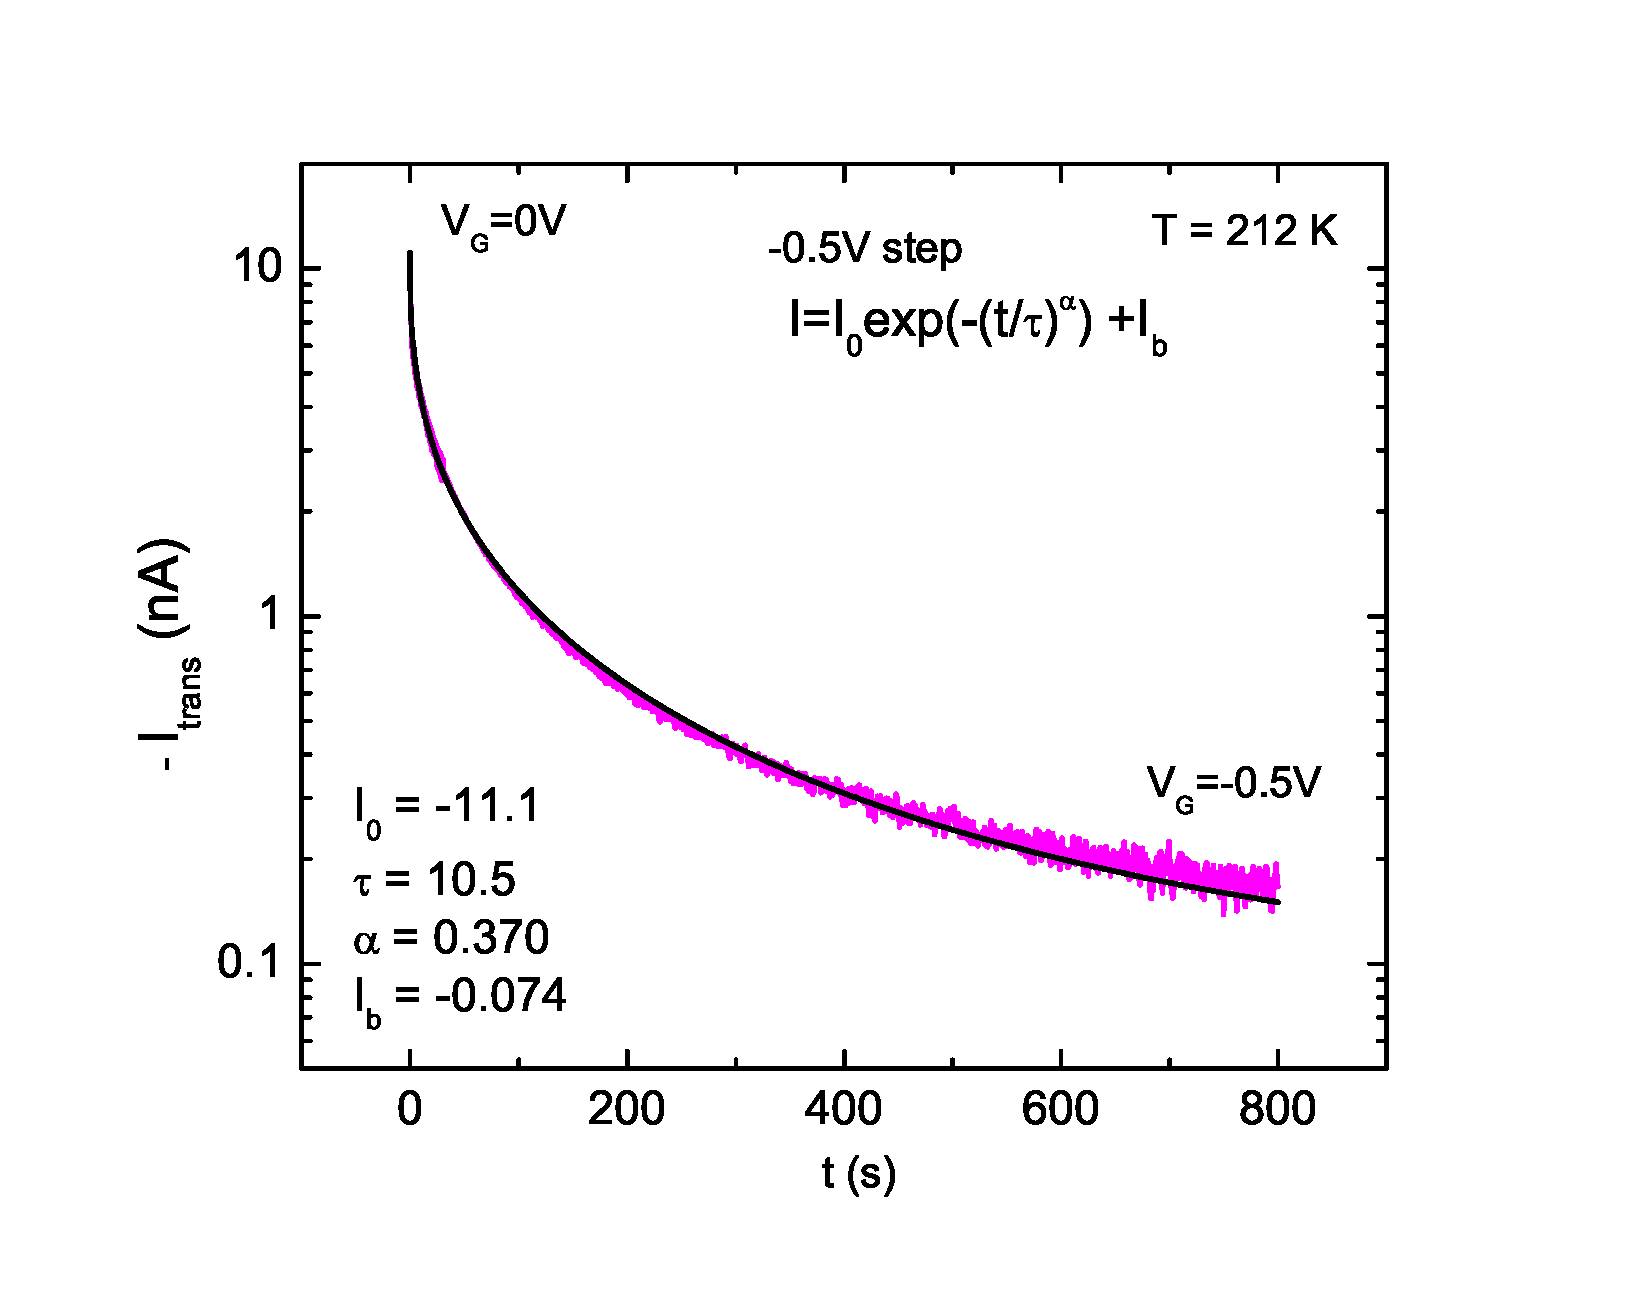
\includegraphics[width=0.65\linewidth]{ch-appendicies/figures/FigTransCurrent.eps}
\caption{\label{figtrans} 
The transient (discharging) current $I_{trans}$ versus time $t$ following a step-change of
$V_G$ from 0 to -5 V at $t$ = 0 at $T$ = 212 K in Sample 3. The observed current fits well to the stretched exponential form
Eq. \ref{Itrans} with the parameters $I_0$ = -11.1 nA, $I_b$ = -0.074 nA, $\alpha$ = 0.37, and $\tau$ = 10.5 s.
$I_b$ is the long-term steady-state background current. 
}
  \end{center}
\end{figure} 


%%%%%%%%%%%%%%%%%%%%%%%%%%%%%%%%%%
%%%%%%%%%%%%%%%%%%%%%%%%%%%%%%%%%%
%%%%%%%%%%%%%%%%%%%%%%%%%%%%%%%%%% FIGURE A2
\begin{figure}[!htbp]
  \begin{center}
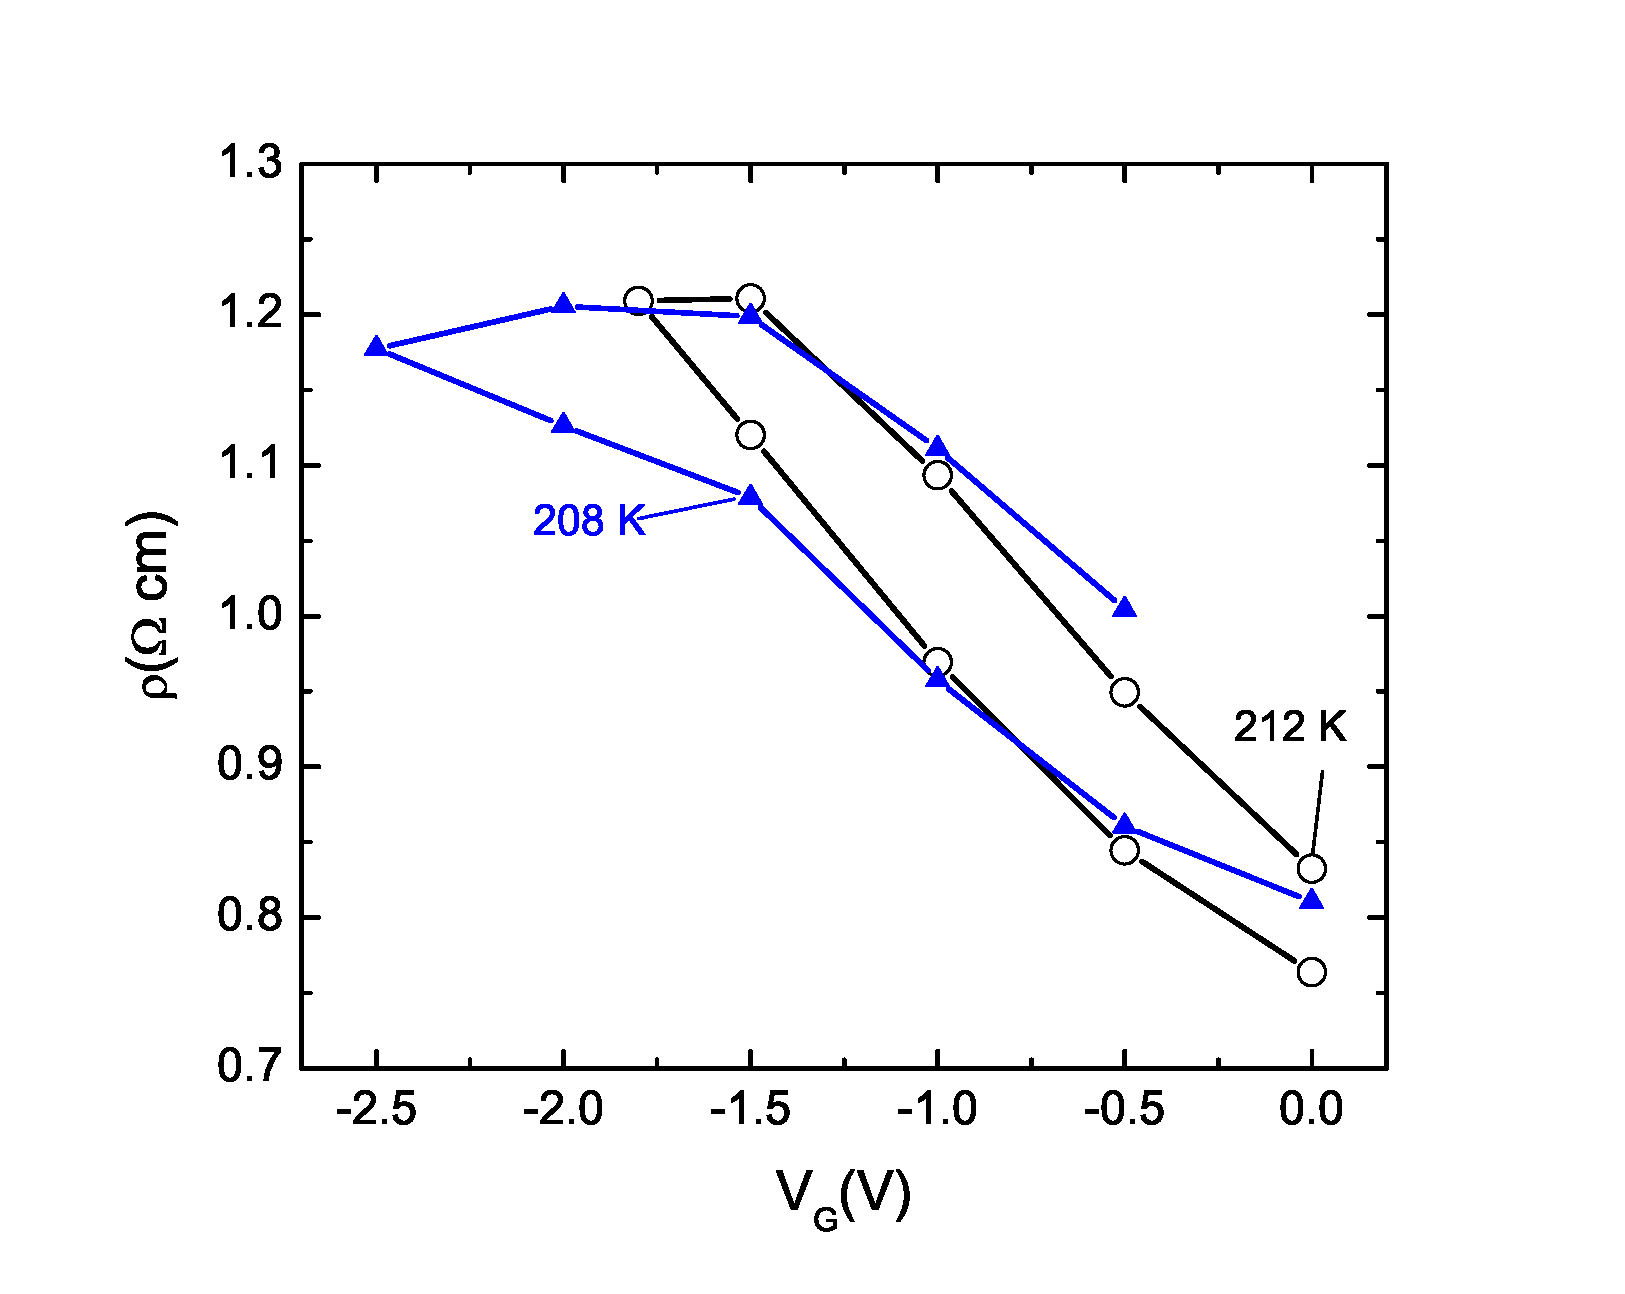
\includegraphics[width=0.7\linewidth]{ch-appendicies/figures/FigRvsVGLowT.eps}
\caption{\label{figRLowT} (color online) 
Apparent hysteretic behavior of $\rho$ vs. $V_G$ observed at temperatures close to the glass transition $T_G$. 
When the gating $T$ is too close to $T_G$, the background quasi-steady state $I_1$ and 
possibilities of chemical reaction are strong suppressed. However, at these temperatures, the ions are almost frozen and it may take a longer time for them to move back. Thus it leads to increased hysteresis in $\rho$ when $V_G$ is cycled (here $T$ = 208 and 212 K). The Hall density $n_H$ shows similarly large hysteresis (not shown). 
As discussed in the text, we show that this apparent low-temperature hysteresis results from incomplete
melting of the ionic liquid.
}
  \end{center}
\end{figure} 



%%%%%%%%%%%%%%%%%%%%%%%%%%%%%%%%%%
%%%%%%%%%%%%%%%%%%%%%%%%%%%%%%%%%%
%%%%%%%%%%%%%%%%%%%%%%%%%%%%%%%%%% FIGURE A3
\begin{figure}[!htbp]
  \begin{center}
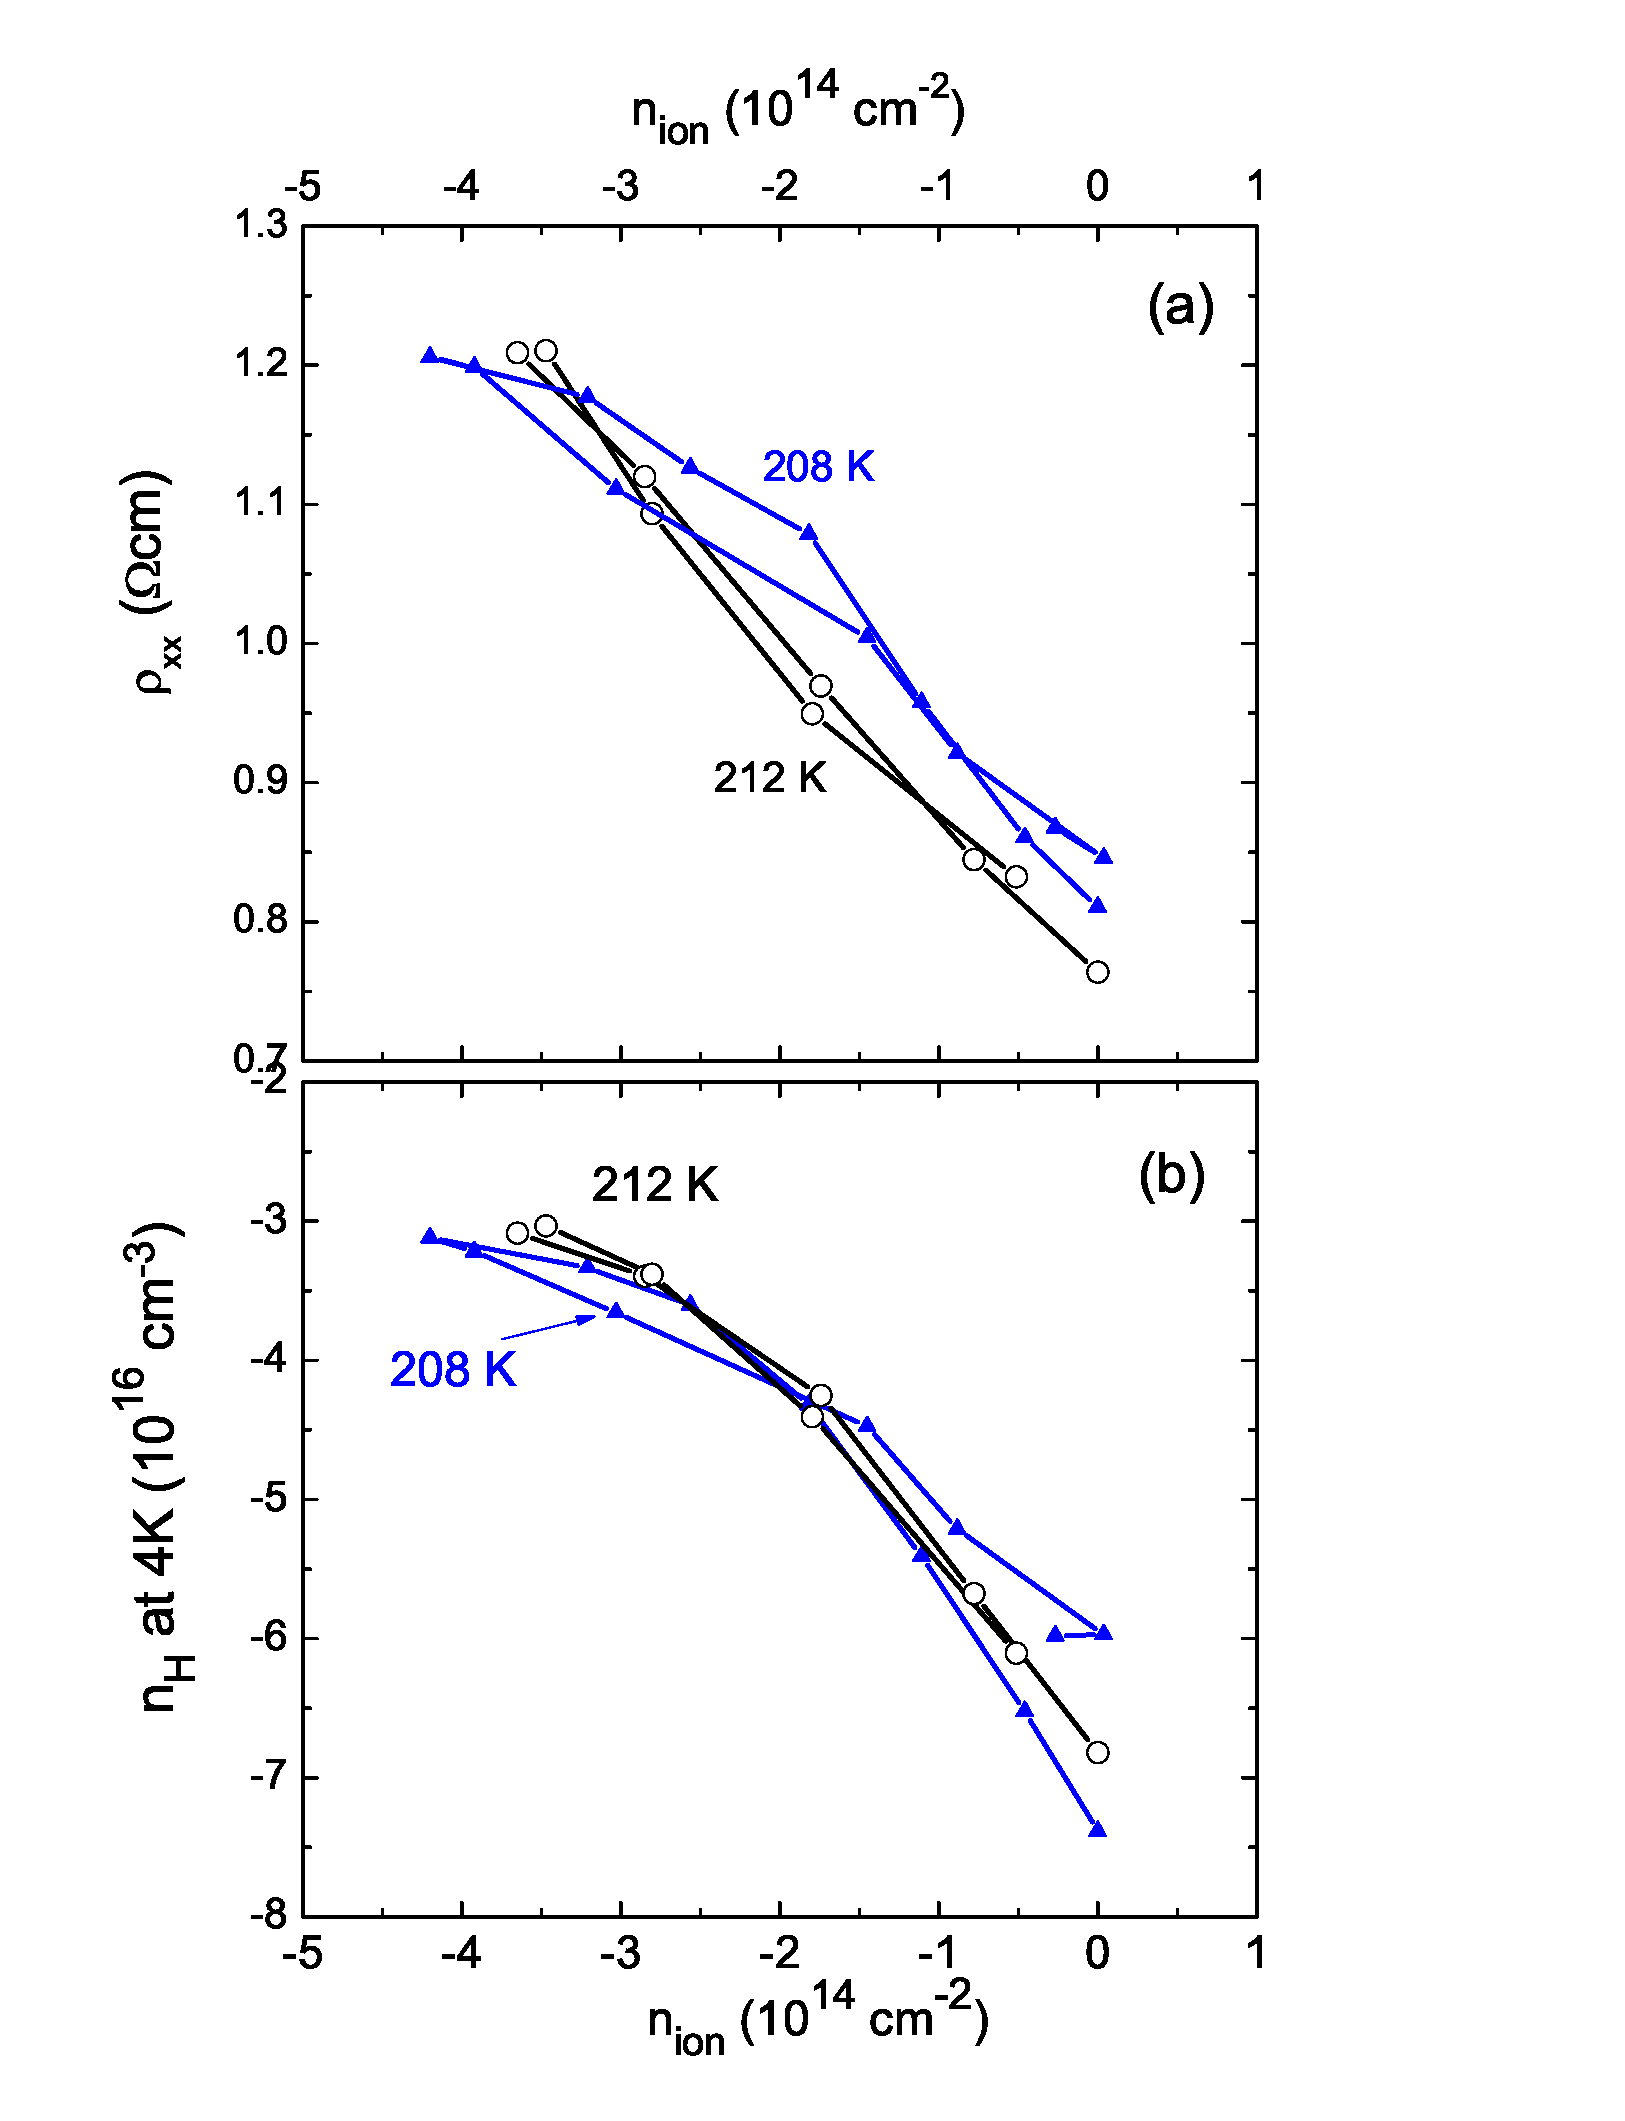
\includegraphics[width=0.7\linewidth]{ch-appendicies/figures/FigRvsNion.eps}
\caption{\label{figNion} (color online) 
Absence of low-temperature hysteresis when $\rho$ and $n_H$ are plotted against $n_{ion}=Q/eA$ (with $A$ = 2.9 mm$^2$), the accumulated charge calculated from the transient charging current.
Replotting the data for $\rho$ in Fig. \ref{figRLowT} versus $n_{ion}$ (instead of $V_G$) removes the hysteresis apparent in Fig. \ref{figRLowT}.
The difference indicates that the hysteretic behavior arises from the variation of $Q$ vs. $V_G$. A possible explanation is that it's hard for the ions to return when they are almost frozen. This figure shows that physically relevant quantities inside the
crystal $\rho$ and $n_H$ are dependent only on $Q$, the accumulated charge in the capacitor. It strongly supports the premise that band-bending 
produces the changes in sample conductance rather than chemical reaction.}
  \end{center}
\end{figure} 




Figure \ref{figRLowT} presents the changes in $\rho$ (Sample 3) as  $V_G$ is cycled between 0 and -2.5 V at 
low temperatures (208 and 212 K) that are close to the glass transition temperature $T_G$. In contrast to Fig. \ref{RvsVG}, we observe
sizeable hysteretic behavior (also in $n_H$, not shown). To show that this is not caused by
chemical reaction (which should be greatly suppressed at low $T$), we have measured the accumulated
$Q(t)$ and found that it displays the same hysteresis (vs. $V_G$). When we plot the changes
in $\rho$ and $n_H$ against $n_{ion} = Q/eA$ (see Fig. \ref{figNion}), 
the hysteretic behavior apparent in Fig. \ref{figRLowT} is largely removed.

This implies that, at these low $T$, a significant portion of the ionic ``solid'' accumulated at the
previous value of $V_G$ fails to melt and flow in response to the new $V_G$. Hence
$Q(t)$ never attains its equilibrium value even at long $t$. This leads 
to strong hysteresis in $Q$ vs. $V_G$. However,
the near-absence of hysteresis in Fig. \ref{figNion} shows that $\rho$ and $n_H$ adjust reversibly to
the non-equilibrium value of $Q$. The key parameter that
causes $\rho$ and $n_H$ to change is the electric-field $E(0^-)$ produced by $Q$ even when it lags
the applied $V_G$. This direct link provides further support for our conclusion that
the dominant effect of changing $Q$ is band-bending instead of chemical reactions.





\chapter{Depletion Layer and Quantum Capacitance in Ionic Liquid Gating Experiments\label{ch:Depletion}}

\begin{figure}[!htbp]
  \begin{center}
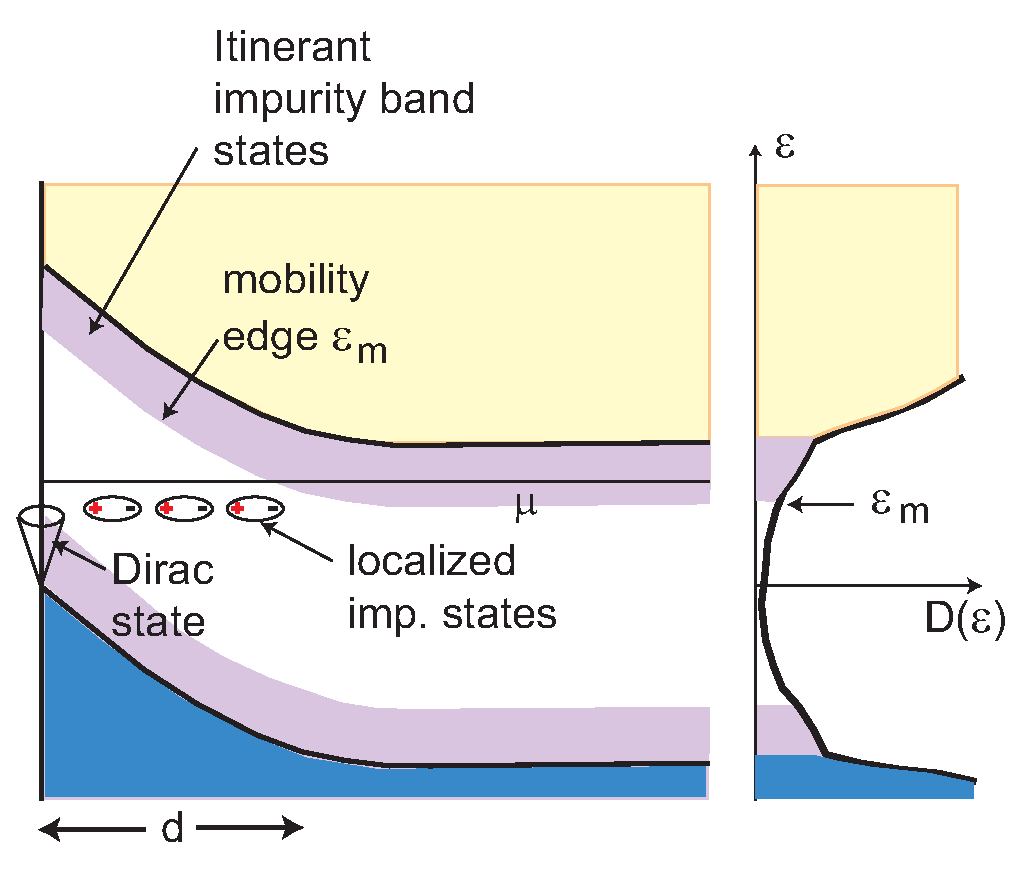
\includegraphics[width=0.65\linewidth]{ch-appendicies/figures/FigImpurityBand.eps}
\caption{\label{figimp}
Model for the impurity band states implied by the liquid-gating experiment. The density of states (DOS)
profile ${\cal D}(\varepsilon)$ across the bulk energy gap is sketched on the right. The impurity-band DOS tapers deep
into the gap, as suggested by STM experiments~\cite{Beidenkopf2011}. Impurity states lying above the mobility edge $\varepsilon_m$ (shaded)
are itinerant with mobility $\mu_b\sim$ 20 cm$^2$/Vs. States below $\varepsilon_m$ are strongly localized at 4 K. 
Near the surface (left sketch), $\varepsilon_m$ is lifted above 
$\mu$ within the depletion layer, substantially decreasing the bulk contribution to the observed $\sigma$ and $\sigma_H$. 
Localized states near the mobility edge (sketched as dipoles) contribute strongly to dielectric screening because of their 
enhanced polarizability.
}
  \end{center}
\end{figure} 


With reference to Fig. \ref{figGate}, the free-charge density profile $\rho(x)$ is comprised of 
4 delta functions $\delta(x)$ and an extended distribution over the depletion width $d$ (which we assume has a flat 
profile expressed by the step-function $\theta(x)$~\cite{Ashcroft}, as shown in Fig. \ref{figGate}(b). Setting the origin $x=0$ at the TI surface, we have
\begin{eqnarray}
\rho(x) &=& -\frac{Q}{A'}\delta(x+s) + \frac{Q}{A'}\delta(x+s-a) -\frac{Q}{A}\delta(x+a) \notag\\
 				&& +\sigma_s \delta(x) + N_ded\,[\theta(x)-\theta(x-d)],
\label{rho}
\end{eqnarray}
where $\sigma_s$ is the surface charge density at the exposed crystal face,
and $N_d$ is the density of ionized donor impurities within the depletion width $d$ (we take $e>0$). The electrostatic potential $\varphi(x)$ is derived from the Poisson equation
\be
-\varepsilon(x) \frac{\partial^2\varphi}{\partial x^2} = \frac{\rho(x)}{\epsilon_0},
\label{phi}
\ee
with $\epsilon_0$ the vacuum permittivity. The dielectric function $\varepsilon(x) = \epsilon_s$ inside the TI ($x>0$). Within the ionic liquid,
$\varepsilon(x) = \epsilon_{liq}$.

Integration of Eq. \ref{phi} gives the profile of $\varphi(x)$ sketched in Fig. \ref{figGate}b. We wish to relate the
charge density $Q/A$ to $\sigma_s$ and $d$.
Setting $\varphi$ and $\partial\varphi/\partial x$ to 0 
deep in the bulk ($x>d$), we have for the $E$-field just to the right of $x = 0$
\be
E(0^+) = -\left(\frac{\partial\varphi}{\partial x}\right)_{0+} = - \frac{N_ded}{\epsilon_0\epsilon_s}.
\label{E0}
\ee
In the flat-profile approximation for $\rho(x)$, Eq. \ref{phi} gives the parabolic variation of $\varphi(x)$ 
\be
\varphi(x) = -\frac{N_de}{2\epsilon_0\epsilon_s}(x-d)^2   \quad (x>0).
\label{varphi}
\ee

Next, we integrate Eq. \ref{phi} between the limits $x = 0^{\pm}$ (bracketing $x =0$) to get
\be
\epsilon_s E(0^+) - E(0^-) = \sigma_s/\epsilon_0.
\label{EE}
\ee
Together, Eqs. \ref{E0} and \ref{EE} give for the $E$-field just to the left of the surface
\be
E(0^-) = -(\sigma_s + N_ded)/\epsilon_0.
\label{E0-}
\ee
This strong $E$-field emanating from the anion charge $-Q$ is only partially screened by the surface charge $\sigma_s$. The remaining
$E$ penetrates a distance $d$ into the bulk until screened by enough ionized donor charge. The lattice polarizability,
expressed by the bulk dielectric constant $\epsilon_s$,
also contributes to the screening. (It is helpful to represent the dielectric screening, alternatively, as a 
bound-surface charge density $\sigma_b = -\epsilon_0(\epsilon_s-1)E(0^+)$ at $x$ = 0. However, this bound charge
should not be included in $\rho(x)$).


Finally, identifying $E(0^-)$ with the $E$-field within the molecular layer, $-Q/A\epsilon_0$, we arrive at the equation
\be
\frac{Q}{A} = N_ded + \sigma_s.
\label{Q}
\ee
We note that Eq. \ref{Q} is independent of $\epsilon_s$.
The charge $Q$ induced by the anions is partitioned between two charge reservoirs which see the same potential drop $V_s = \varphi(0)$ relative to the 
ground at $x=+\infty$. Hence, as shown in Fig. \ref{figGate}c, we regard the two charge reservoirs 
as two capacitors in parallel, namely the 
quantum capacitance~\cite{Luryi}
\be
C_q = \frac{\sigma_s}{\varphi(0)} = e^2\frac{dn_s}{d\mu},
\label{Cq}
\ee 
and the depletion-layer capacitance 
\be
C_d = N_dedA/\varphi(0).
\label{Cd}
\ee
Whereas in graphene, the quantum capacitance is readily resolved,
here it is shunted by the large $C_d$.

The parallel combination $C_q+C_d$ is in series with the ionic-liquid capacitor $C_0$ (the series combination of the cation and anion capacitors). The
voltage drop across $C_0$ is $V_G-V_s$.


\vspace{3mm}
%\noindent

We discuss a scenario in which a strongly enhanced electronic polarizability arises 
within the depletion layer. Figure \ref{figimp} is a sketch of the band bending near the surface. 
As shown, the chemical potential $\mu$ in the bulk lies just below the bottom of the conduction band.
The right panel plots the density of states ${\cal D}(\varepsilon)$ in a cut in the bulk.
The impurity band is comprised of ``tails'' of ${\cal D}(\varepsilon)$ which taper downwards (upwards) from the
conduction band (valence band)~\cite{Beidenkopf2011}. At 4 K, the mobility edge
$\varepsilon_m$ sharply divides states that are itinerant (closer to the gap edge) from 
the states that are localized. Electrons in the itinerant states diffuse with the observed mobility $\mu_b\sim$ 20 cm$^2$/Vs. 
In an $E$-field strong enough to cause band bending, 
$\varepsilon_m$ is lifted above $\mu$ within the depletion region of width $d$. Occupied states within this 
region are strongly localized, so they do not contribute to the observed conductivity or Hall effect. 
However, because the localization length $\xi_{loc}$ diverges as $\varepsilon\to \varepsilon_m$ from below, 
the localized states have a greatly enhanced electronic polarizability. 
The electronic component of the dielectric screening parameter will be much
larger than that from the lattice polarizability.

%\chapter{Resistivity and Conductivity Tensors from Boltzmann Equation in Tilted Magnetic Field\label{ch:Boltzmann}}

%\subsection{Resistivity and conductivity tensors from Boltzmann equation in tilted field}
In this section, we will show that the above MR results of our Na$_3$Bi samples at different directions of $\bf B$ are not expected from the conventional semiclassical, one-band transport theory in a tilted field. For a single anisotropic band, the Boltzmann equation is
\be
e{\bf E\cdot v}\frac{\partial f^0_{\bf k}}{\partial \epsilon_{\bf k}} + e{\bf v\times B}\cdot\frac{\partial g_{\bf k}}{\partial {\bf k}} 
= -\frac{g_{\bf k}}{\tau},
\label{Boltz}
\ee
with $e$ the charge, $\bf E$ the electric field, $\bf v = \partial\epsilon_{\bf k}/\hbar\partial {\bf k}$ the band velocity, $g_{\bf k}$ the leading correction to the equilibrium distribution function $f^0_{\bf k}$, and $\tau$ the relaxation time. Suppose the magnetic field is in the $x$-$z$ plane, i.e. ${\bf B} = (B_1, 0, B_3)$. Using the \emph{ansatz} with $\bf u$ the drift velocity
\be
g_{\bf k} = -{\bf u\cdot k}\frac{\partial f^0_{\bf k}}{\partial \epsilon_{\bf k}},
\ee
and the effective mass matrix
\begin{eqnarray}
\hat{m} = \left[   \begin{array}{ccc}
		m_1   &   0   &   0 \\
		0      &    m_2 &   0 \\
		0     &    0     &   m_3   \end{array}\right]
\end{eqnarray}
we can solve Eq. \ref{Boltz} to get the resistivity tensor ($n$ is the carrier density)
\begin{eqnarray}
\hat{\rho} = 
						\left[  	\begin{array}{ccc}
								\rho_1	&  -B_3/ne   &   0  \\
								B_3/ne  &   \rho_2   &   -B_1/ne \\
								0          &   B_1/ne   &   \rho_3   
								\end{array}
								\right].
				\label{rhoij}
				\end{eqnarray}
				

Inverting $\hat\rho$, we obtain the conductivity tensor 
\begin{eqnarray}
\hat{\sigma} = 
						\frac{1}{\Delta}\left[  	\begin{array}{ccc}
								\sigma_1(1+\mu_1\mu_3 B_1^2)  &  \sigma_1\mu_2B_3   &   \sigma_2\mu_1\mu_3 B_1B_3 \\
								 -\sigma_1\mu_2B_3									&   \sigma_2   									&   \sigma_2\mu_3B_1   \\
								\sigma_2\mu_1\mu_3 B_1B_3     &    -\sigma_2\mu_3B_1      &   \sigma_3(1+\mu_1\mu_2B_3^2)
								\end{array}
								\right]
				\label{Sij}
				\end{eqnarray}
where the zero-field conductivities and resistivities are defined by $\sigma_i = 1/\rho_i = ne\mu_i $ in terms of the anisotropic
mobilities $\mu_i = e\tau/m_i$. The determinant $\Delta$ equals $(1+\mu_2\mu_3 B_1^2+ \mu_1\mu_2 B_3^2)$.

An important conclusion of the above calculations is that, despite the anisotropy and the tilted field direction, the longitudinal resistivity 
$\rho_{xx}$ (the three diagonal terms) is strictly independent of $\bf B$ (meaning the Hall E-field perfectly balances the Lorentz force). In the limit $B_3\to 0$ (or $\theta\to 0$ in Fig. \ref{figPolar4}C,D), the longitudinal conductivity $\sigma_{xx}$ acquires a mild field dependence that vanishes if $\mu_1 = \mu_2 = \mu_3$. It never diverges as $1/\sin\theta$ or any other form.

Equations \ref{rhoij} and \ref{Sij} also apply to the geometry with $\bf B$ in the $x$-$y$ plane (Fig. 3 and Fig. 4A,B of main text) if we exchange the axes $y\leftrightarrow z$.

%\chapter{Splitting of Generated Weyl Nodes of a Dirac Semimetal in a Magnetic Field\label{ch:WeylSplit}}


%\subsection{Splitting of generated Weyl nodes of a Dirac semimetal in a magnetic field}
In this section, we will discuss a crucial problem of 3D Dirac semimetals, i.e. how much shift can the Weyl nodes have in a magnetic field when they are generated from the Dirac nodes at zero field. To solve this problem,we leverage the model introduced by Wang \etal~\cite{Wang2012} (see also Jeon \etal~\cite{Jeon2014}), and estimate the shift in the Weyl nodes induced by the magnetic field $\bf B$ as follows. In a field $\bf B\parallel \hat{z}$, we have ${\bf k \to \Pi} = {\bf k} - e{\bf A}$, with the vector potential ${\bf A} = xB{\bf \hat{y}}$. The wavevector $\bf k$ is measured relative to the Dirac node. Neglecting the off-diagonal corrections in the full $4\times4$ Hamiltonian, the
$2\times2$ Hamiltonian for the ``up'' Weyl node has the form 
\begin{eqnarray}
H_+ = \hbar v\left[\begin{array}{cc}
						\Pi_z   &  \Pi_+   \\
						\Pi_-   &   -\Pi_z  
						\end{array}\right]
						-\mu_B B \left[\begin{array}{cc}
						g_s   &   0   \\
						0      &   g_p  
						\end{array}\right],
						\label{H1}
						\end{eqnarray}
where $\Pi_{\pm} = \Pi_x \pm i\Pi_y$ and $\mu_B$ is the Bohr magneton. Expressing the $g$-factors $g_s$ and $g_p$ (which are distinct) of the starting atomic orbitals $|S,\pm\rangle$ and $|P,\pm\rangle$ as $g_s = g_m + \delta g$ and $g_p = g_m - \delta g$, we have the Hamiltonian 
\be
H_+ = v{\bf \Pi\cdot }\boldsymbol{\tau} - g_m\mu_B B {\bf 1}- \delta g\mu_B B \tau_3,
\label{H2}
\ee
where $\tau_i$ are the Pauli matrices in orbital space.
By transforming the $\Pi_\pm$ to raising and lowering operators $a^\dagger$ and $a$, with $\ell_B$ the magnetic length,
\be
\Pi_+ = \frac{\sqrt{2} a^\dagger}{\ell_B}, \quad \Pi_- = \frac{\sqrt{2} a}{\ell_B}
\label{Pi}
\ee
we diagonalize $H_+$ to obtain the eigenenergy of the $n^{th}$ Landau level
\be
E_n(k_z) = -g_m\mu_B B \pm \sqrt{ \frac{2n\hbar^2 v^2}{\ell_B^2} + (\hbar vk_z -\delta g\mu_BB)^2}.
\label{En}
\ee
Setting the second term under the square root to zero, we obtain $\Delta k = \delta g\mu_B B/\hbar v$.
This is used in the main text to estimate the shift. 

The term $-g_m\mu_B B$ in Eq. \ref{En} leads to pronounced deviation of the index plot from a straight line if $|g_m|\gg 1$, consistent with the deviation in Fig. \ref{figSdH}.


%\chapter{Printing and Binding\label{ch:printing}}

\section{Printing}

For the library copies of your dissertation, you must use archival quality printing and binding. This means acid-free paper, containing at least 25\% cotton fiber. Triangle Repocenter on Nassau Street in Princeton offers both 25\% cotton paper and 100\% cotton paper. Most people choose the 25\% cotton paper, and this is generally recommended by the binders. The 100\% copy paper is somewhat thicker and the extra expense is unnecessary. 

Triangle offers online submission of your printing and binding order at: \url{http://triangleprinceton.com/collegiatebinding/thesis/}. If you request binding from them, they will deliver the paper copies to Smith-Shattuck Bookbinding for you and allow you to pick up the completed copies at their store on Nassau Street. The whole process takes 2-3 business days, but check with them in advance during the busy thesis-printing season in April and May. 

Currently, your printed and bound dissertation copies can be single spaced. Only the electronic copy submitted to ProQuest must be double spaced. All copies must be printed single-sided, with specific margins. 

\section{Binding}

An archival-quality sewn binding is required for the library copies of your dissertation. Smith-Shattuck Bookbinding is highly recommended, and is used by most students. Triangle Repocenter will send your copies there for you, greatly simplifying the process, but you can call Smith-Shattuck with special requests. 

The ``library standard'' sewn binding is sufficient for the copies to be sent to Mudd Library. It uses a black buckram cloth cover, which is the most popular option. For extra copies for yourself and your family members, you can choose ``buckram roundback binding'', which adds decorative lines on the spine, and printing of the title and author on the front cover. For a small additional fee, you can include the Princeton University shield on the front cover and a ribbon bookmark. Leather covers are also available. See Smith-Shattuck's website for more details at: \url{http://www.thesisbookbinding.com/}. 


% Make the bibliography single spaced
\singlespacing
\bibliographystyle{plain}
%\bibliographystyle{unsrt}

% add the Bibliography to the Table of Contents
\cleardoublepage
\ifdefined\phantomsection
  \phantomsection  % makes hyperref recognize this section properly for pdf link
\else
\fi
\addcontentsline{toc}{chapter}{Bibliography}

% include your .bib file

\newpage
%\bibliographystyle{unsrt}
%\bibliographystyle{plain}
\bibliography{thesis}


\end{document}

